%%%%%%%%%%%%%%%%%%%%%%%%%%%%%%%%%%%%%%%%%
% kaobook
% LaTeX Template
% Version 1.2 (4/1/2020)
%
% This template originates from:
% https://www.LaTeXTemplates.com
%
% For the latest template development version and to make contributions:
% https://github.com/fmarotta/kaobook
%
% Authors:
% Federico Marotta (federicomarotta@mail.com)
% Based on the doctoral thesis of Ken Arroyo Ohori (https://3d.bk.tudelft.nl/ken/en)
% and on the Tufte-LaTeX class.
% Modified for LaTeX Templates by Vel (vel@latextemplates.com)
%
% License:
% CC0 1.0 Universal (see included MANIFEST.md file)
%
%%%%%%%%%%%%%%%%%%%%%%%%%%%%%%%%%%%%%%%%%

%----------------------------------------------------------------------------------------
%	PACKAGES AND OTHER DOCUMENT CONFIGURATIONS
%----------------------------------------------------------------------------------------

\documentclass[
	fontsize=10pt, % Base font size
	twoside=false, % Use different layouts for even and odd pages (in particular, if twoside=true, the margin column will be always on the outside)
	%open=any, % If twoside=true, uncomment this to force new chapters to start on any page, not only on right (odd) pages
	%chapterprefix=true, % Uncomment to use the word "Chapter" before chapter numbers everywhere they appear
	%chapterentrydots=true, % Uncomment to output dots from the chapter name to the page number in the table of contents
	numbers=noenddot, % Comment to output dots after chapter numbers; the most common values for this option are: enddot, noenddot and auto (see the KOMAScript documentation for an in-depth explanation)
	%draft=true, % If uncommented, rulers will be added in the header and footer
	%overfullrule=true, % If uncommented, overly long lines will be marked by a black box; useful for correcting spacing problems
]{kaobook}

% Set the language
\usepackage[english]{babel} % Load characters and hyphenation
\usepackage[english=british]{csquotes} % English quotes

% Load packages for testing
\usepackage{blindtext}
%\usepackage{showframe} % Uncomment to show boxes around the text area, margin, header and footer
%\usepackage{showlabels} % Uncomment to output the content of \label commands to the document where they are used

% Load the bibliography package
\usepackage[style=alphabetic]{styles/kaobiblio}
\addbibresource{main.bib} % Bibliography file

% Load mathematical packages for theorems and related environments. NOTE: choose only one between 'mdftheorems' and 'plaintheorems'.
\usepackage{styles/mdftheorems}
%\usepackage{styles/plaintheorems}

\usepackage{mathpartir}
\usepackage{dirtree}
\usepackage{xspace}
\usepackage{tikz}
\usepackage{fancyvrb}
\usepackage{bussproofs,proof}

\newcommand{\newfrac}[2] {
        \frac
                {#1}
                {#2 \rule{0pt}{11pt}}
}
\newcommand{\newinfrule}[2] {
  \ensuremath{\newfrac
    {\displaystyle #1}
    {\displaystyle #2}}
}
\newcommand{\rulesep}{\quad}


\usetikzlibrary{arrows}
\tikzset{
  treenode/.style = {align=center, inner sep=0pt, text centered},
  arn_u/.style = {treenode, circle, black, draw=black, text width=0.8cm, line width=0.25mm},
  arn_w/.style = {treenode, circle, white, draw=white, text width=0.8cm, line width=0.25mm},
  arn_nc/.style = {treenode, circle, black, draw=white, text width=0.8cm, line width=0.25mm},
}

\newcommand{\shorteq}{\code{=}}

\newcommand{\lang}{}
\newcommand{\plang}{}
\newcommand{\code}[1]{\texttt{#1}}
\newcommand{\cx}{\code{x}}
\newcommand{\cy}{\code{y}}
\newcommand{\cz}{\code{z}}
\newcommand{\cf}{\code{f}}
\newcommand{\cv}{\code{v}}

\newcommand{\pto}{\mathrel{\ooalign{\hfil$\mapstochar$\hfil\cr$\to$\cr}}}
\newcommand{\finto}{\stackrel{\mbox{\tiny fin}}{\pto}}
\newcommand{\embox}[1]{\mbox{\emph{#1}}}
\newcommand{\dom}[1]{\embox{Domain}(#1)}
\newcommand{\iadd}{+_{{}_{\mathbb{Z}}}}
\newcommand{\isub}{-_{{}_{\mathbb{Z}}}}

\newcommand{\fundef}[3]{\textsf{def}\ #1(#2)\shorteq#3}
\newcommand{\clov}[3]{\langle\efun{#1}{#2},#3\rangle}
\newcommand{\contv}[2]{\langle#1,#2\rangle}
\newcommand{\exprv}[2]{(#1,#2)}
\newcommand{\eadd}[2]{#1+#2}
\newcommand{\esub}[2]{#1-#2}
\newcommand{\ebind}[3]{\textsf{val}\ #1\shorteq#2\ \textsf{in}\ #3}
\newcommand{\evcc}[2]{\textsf{vcc}\ #1\ \textsf{in}\ #2}
\newcommand{\efun}[2]{\lambda#1.#2}
\newcommand{\efunt}[3]{\lambda#1{:}#2.#3}
\newcommand{\eapp}[2]{#1\ #2}
\newcommand{\eappfo}[2]{#1(#2)}
\newcommand{\erec}[4]{\textsf{def}\ #1(#2)\shorteq#3\ \textsf{in}\ #4}
\newcommand{\eifz}[3]{\textsf{if0}\ #1\ #2\ #3}
\newcommand{\eif}[3]{\textsf{if}\ #1\ #2\ #3}
\newcommand{\eref}[1]{\textsf{box}\ #1}
\newcommand{\ederef}[1]{!#1}
\newcommand{\eset}[2]{#1{:}\shorteq#2}
\newcommand{\eseq}[2]{#1;#2}
\newcommand{\erect}[6]{\textsf{def}\ #1(#2{:}#3){:}#4\shorteq#5\ \textsf{in}\ #6}

\newcommand{\tnum}{\textsf{num}}
\newcommand{\tfun}{\textsf{fun}}
\newcommand{\tarrow}[2]{#1\rightarrow#2}

\newcommand{\mtk}{\square}
\newcommand{\evalk}[2]{#1\vdash#2::}
\newcommand{\evalkd}[1]{\evalk{\sigma}{#1}}
\newcommand{\evalke}[1]{\evalk{\emptyset}{#1}}
\newcommand{\addk}{(+)::}
\newcommand{\subk}{(-)::}
\newcommand{\appk}{(@)::}

\newcommand{\mts}{\blacksquare}
\newcommand{\conss}[1]{#1::}

\newcommand{\eval}[3]{#1\vdash#2\Rightarrow#3}
\newcommand{\evaln}[3]{\ensuremath{#2} evaluates to \ensuremath{#3} under
\ensuremath{#1}\xspace}
\newcommand{\evald}[2]{\eval{\sigma}{#1}{#2}}
\newcommand{\evaldn}[2]{\evaln{\sigma}{#1}{#2}}
\newcommand{\evale}[2]{\eval{\emptyset}{#1}{#2}}

\newcommand{\typeof}[3]{#1\vdash#2:#3}
\newcommand{\typeofd}[2]{\typeof{\Gamma}{#1}{#2}}
\newcommand{\typeofe}[2]{\typeof{\emptyset}{#1}{#2}}
\newcommand{\typeofn}[3]{the type of \ensuremath{#2} is
\ensuremath{#3} under \ensuremath{#1}\xspace}
\newcommand{\typeofdn}[2]{\typeofn{\Gamma}{#1}{#2}}
\newcommand{\typeofnc}[3]{The type of \ensuremath{#2} is
\ensuremath{#3} under \ensuremath{#1}\xspace}
\newcommand{\typeofdnc}[2]{\typeofnc{\Gamma}{#1}{#2}}

\newcommand{\stricte}[2]{#1\Downarrow#2}
\newcommand{\stricten}[2]{\ensuremath{#1} strictly evaluates to \ensuremath{#2}}

\newcommand{\seval}[5]{#1,#2\vdash#3\Rightarrow#4,#5}
\newcommand{\sevaln}[5]{
  \ensuremath{#3} evaluates to \ensuremath{#4} and changes the store from
  \ensuremath{#2} to \ensuremath{#5} under \ensuremath{#1}\xspace
}
\newcommand{\sevald}[4]{\seval{\sigma}{M_{#1}}{#2}{#3}{M_{#4}}}
\newcommand{\sevaldn}[4]{\sevaln{\sigma}{M_{#1}}{#2}{#3}{M_{#4}}}
\newcommand{\sevale}[3]{\seval{\emptyset}{\emptyset}{#1}{#2}{#3}}

\newcommand{\semanticrule}[2]{
\vspace{1em}
\textbf{Rule \textsc{#1}}\\
#2
\vspace{1em}
}
\newcommand{\typerule}[2]{
\vspace{1em}
\textbf{Rule \textsc{#1}}\\
#2
\vspace{1em}
}
\newcommand{\tand}{\text{ and }}

\newcommand{\inred}[1]{{\color{red}{#1}}}
\newcommand{\mtt}[1]{\mbox{\texttt{#1}}}
\newcommand{\finmap}[2]{#1 \xrightarrow[]{\text{fin}} #2}
\newcommand{\sblank}{\fbox{\rule{1.5in}{0pt}\rule{0pt}{0.2in}}}
\newcommand{\mblank}{\fbox{\rule{4in}{0pt}\rule{0pt}{0.3in}}}
\newcommand{\lblank}{~~~\fbox{\rule{5in}{0pt}\rule{0pt}{0.5in}}~~~}
\newcommand{\lmblank}{~~~\fbox{\rule{5in}{0pt}\rule{0pt}{0.39in}}~~~}
\newcommand{\MNSC}{\code{mini-Scala}\xspace}
\newcommand{\Space}[1]{\vspace{#1ex}}
\newcommand{\typed}[2]{\Gamma\vdash#1:#2}
\newcommand{\rom}[1]{\uppercase\expandafter{\romannumeral #1\relax}}
\newcommand{\wfd}[1]{\Gamma\vdash#1}
\newcommand{\subt}[2]{#1<:#2}
\newcommand{\Dom}[1]{\mbox{Domain}(#1)}
\newcommand{\clo}[3]{\langle\lambda #1.#2,#3\rangle}
\newcommand{\etfun}[2]{\Lambda#1.#2}
\newcommand{\etapp}[2]{#1[#2]}
\newcommand{\numt}{\textsf{num}}
\newcommand{\synsep}{\ \ |\ \ }
\newcommand{\seq}{%
    \settowidth{\@tempdima}{-}% Width of hyphen
      \resizebox{\@tempdima}{\height}{=}%
      }


\makeindex[columns=3, title=Alphabetical Index, intoc] % Make LaTeX produce the files required to compile the index

\makeglossaries % Make LaTeX produce the files required to compile the glossary

\makenomenclature % Make LaTeX produce the files required to compile the nomenclature

% Reset sidenote counter at chapters
%\counterwithin*{sidenote}{chapter}

%----------------------------------------------------------------------------------------

\begin{document}

%----------------------------------------------------------------------------------------
%	BOOK INFORMATION
%----------------------------------------------------------------------------------------

% \titlehead{The \texttt{kaobook} class}
% \subject{Use this document as a template}

% \title[Example and documentation of the {\normalfont\texttt{kaobook}} class]{Example and documentation \\ of the {\normalfont\texttt{kaobook}} class}
\title{Introduction to Programming Languages}

% \author[Federico Marotta]{Federico Marotta \thanks{A \LaTeX\ lover}}
\author{Jaemin Hong and Sukyoung Ryu}

% \date{}

% \publishers{An Awesome Publisher}

%----------------------------------------------------------------------------------------

\frontmatter % Denotes the start of the pre-document content, uses roman numerals

%----------------------------------------------------------------------------------------
%	OPENING PAGE
%----------------------------------------------------------------------------------------

%\makeatletter
%\extratitle{
%	% In the title page, the title is vspaced by 9.5\baselineskip
%	\vspace*{9\baselineskip}
%	\vspace*{\parskip}
%	\begin{center}
%		% In the title page, \huge is set after the komafont for title
%		\usekomafont{title}\huge\@title
%	\end{center}
%}
%\makeatother

%----------------------------------------------------------------------------------------
%	COPYRIGHT PAGE
%----------------------------------------------------------------------------------------

\makeatletter
\uppertitleback{\@titlehead} % Header

\lowertitleback{
  % \textbf{License}\\
	\copyright2021 Jaemin Hong and Sukyoung Ryu

  \medskip

  All rights reserved. No part of this book may be reproduced in any form by any
  electronic of mechanical means (including photocopying, recording, or
  information storage and retrieval) without permission in writing from the
  authors.

  % \medskip

  % \textbf{Published Date}\\
  % \today
}
\makeatother

%----------------------------------------------------------------------------------------
%	DEDICATION
%----------------------------------------------------------------------------------------

% \dedication{
% 	The harmony of the world is made manifest in Form and Number, and the heart and soul and all the poetry of Natural Philosophy are embodied in the concept of mathematical beauty.\\
% 	\flushright -- D'Arcy Wentworth Thompson
% }

%----------------------------------------------------------------------------------------
%	OUTPUT TITLE PAGE AND PREVIOUS
%----------------------------------------------------------------------------------------

% Note that \maketitle outputs the pages before here

% If twoside=false, \uppertitleback and \lowertitleback are not printed
% To overcome this issue, we set twoside=semi just before printing the title pages, and set it back to false just after the title pages
\KOMAoptions{twoside=semi}
\maketitle
\KOMAoptions{twoside=false}

%----------------------------------------------------------------------------------------
%	PREFACE
%----------------------------------------------------------------------------------------

%\input{chapters/preface.tex}
\setchapterpreamble[u]{\margintoc}
\chapter{Acknowledgement}
\labch{acknowledgement}

The contents of this book are based on the KAIST \textit{Programming Languages}
course. We thank PLT\sidenote{\url{https://racket-lang.org/people.html}} since
the course referred to many materials from PLT in the beginning.
We also thank every student who took the
course before. We have learned many things from the interaction with the
students, and those lessons have affected various parts of the book. In
addition, we thank all the previous and current teaching assistants of the
course. They gave opinions to the course and wrote some of the exercises in the
book. Especially, Jihyeok Park highly contributed to the course, and Jihee Park
helped us edit the exercises.

We would be delighted to receive comments and corrections, which may be sent to
\code{jaemin.hong@kaist.ac.kr}. We thank in advance everyone who will contribute
to the book in the future.


%----------------------------------------------------------------------------------------
%	TABLE OF CONTENTS & LIST OF FIGURES/TABLES
%----------------------------------------------------------------------------------------

\begingroup % Local scope for the following commands

% Define the style for the TOC, LOF, and LOT
%\setstretch{1} % Uncomment to modify line spacing in the ToC
%\hypersetup{linkcolor=blue} % Uncomment to set the colour of links in the ToC
\setlength{\textheight}{23cm} % Manually adjust the height of the ToC pages

% Turn on compatibility mode for the etoc package
\etocstandarddisplaystyle % "toc display" as if etoc was not loaded
\etocstandardlines % toc lines as if etoc was not loaded

\tableofcontents % Output the table of contents

% \listoffigures % Output the list of figures

% Comment both of the following lines to have the LOF and the LOT on different pages
% \let\cleardoublepage\bigskip
% \let\clearpage\bigskip

% \listoftables % Output the list of tables

\endgroup

%----------------------------------------------------------------------------------------
%	MAIN BODY
%----------------------------------------------------------------------------------------

\mainmatter % Denotes the start of the main document content, resets page numbering and uses arabic numbers
\setchapterstyle{kao} % Choose the default chapter heading style

\setchapterpreamble[u]{\margintoc}
\chapter{Introduction}
\labch{introduction}

What is a programming language?

The simplest answer is ``it is a language used for programming.'' However, this
answer does not help us understand programming languages. We need a better
question to get a better answer.

What does a programming language consist of?

There is a good answer for this question: ``in a narrow sense, a programming
language consists of syntax and semantics, and in a broad sense, it additionally
has a standard library and an ecosystem.''

Syntax and semantics are principal concepts to understand programming languages.
Syntax determines how a language looks like, and semantics fills the inside. If
we consider a programming language as a human, we can say that syntax is one’s
appearance, and semantics is one’s thoughts. Programmers write programs
according to syntax. Syntax decides characters used in source code. Once programs
are written, semantics decides what each program does. Without semantics, all
the programs are useless. Programs can work as being expected only after
semantics determines the meaning of them. A programming language with syntax and
semantics is complete. Programmers using that language can write programs with
the syntax and execute the programs with the semantics. From a theoretical
perspective, syntax and semantics are all of a programming language.

For programmers, syntax and semantics are not the only elements of a programming
language. First, the standard library of a language is another element. The
standard library provides various utilities required by applications: data
structures like lists and maps, functions handling file and network IO, and so
on. The standard library is like clothes for humans. A human without clothes is
a human; a programming language without a standard library is a programming
language. At the same time, clothes are important to humans as they make bodies
warm and protect bodies from dangerous objects. Similarly, a standard library is
important to a programming language as it supplies diverse functionalities for
applications. Each person wears clothes different from others, and each language
puts different things from other languages in its standard library. Some
languages include lots of utilities in their standard libraries, while others
include much less. Some languages treat lists and maps as built-in concepts in
their semantics, while others define them with other primitives in their standard libraries.
Programmers avoid using a language without a standard library because such a
language increases the effort to write programs.

Another important element to programmers is the ecosystem of a programming
language. The ecosystem includes everything related to the language: developers
and companies using the language, third-party libraries written in the language,
and so on. It is like a society for humans. If many programmers and companies
use a programming language, one can easily get help and find complementary
materials by using the same language. There will be more chances of cooperative
work and employment, too. Third-party libraries also take important roles in
software development. The standard library offers only general facilities and
often lacks domain-specific features. When a required functionality cannot be
found in the standard library, a third-party library can provide the exact
functionality. For these reasons, the ecosystem of a programming language is
important to programmers.

Practically, the standard library and the ecosystem of a language are important
elements. Unlike syntax and semantics, they are not essential. A programming
language can exist even without its standard library and ecosystem. However,
developers take standard libraries and ecosystems into account as well as syntax and
semantics to choose languages they use. From a practical perspective, a
programming language consists of syntax, semantics, a standard library, and an
ecosystem.

This book is not for helping readers use a specific programming language. It
does not recommend a specific programming language, either. This book helps
readers learn new programming languages easily. You can acquaint any programming
languages once you completely read and understand this book. Obviously, this
goal cannot be achieved if the book discusses various languages separately. It
is possible only by discussing the underlying principles of every programming
language.

The principles of programming languages can be found from their semantics. Each
language seems very different from the others, but it is actually not the case.
Precisely speaking, their insides are quite the same, while their appearances
look different. They look different because their syntax and standard libraries,
which determine the appearances, are different. However, their insides, the
semantics, fundamentally share the same mathematical principles. If you
understand essential concepts residing in the semantics of multiple languages,
it is easy to understand and learn new languages.

People who know the key principles and can separate the elements of a language
can easily learn programming languages. As an analogy, consider a man learning
how to use a computer. It is a big problem if he cannot distinguish a keyboard
from a computer. For example, he thinks ``to say hello, my right index finger
presses the keyboard, my left middle finger presses the keyboard, my right ring
finger presses the keyboard three times.'' If the layout of the keyboard changes,
he should learn the whole computer again. On the other hand, if he knows that a
keyboard is just a tool to input text, he will less suffer from the change of
the keyboard layout. As he thinks ``to say hello, I press H, E, L, L, and O,'' he
does not need to learn the whole computer again. Of course, he should learn the
new keyboard layout, but it will be much easier. In addition, it is
straightforward to apply his knowledge to do new things. For example, he will
easily figure out ``to say lol, I press L, O, and L.'' If he does not distinguish
a keyboard from a computer, he cannot find any common principles between saying
hello and saying lol. Learning programming languages is the same. People who
cannot distinguish syntax and semantics believe that they should learn the whole
language again when the syntax changes. On the other hand, people who can
distinguish syntax and semantics know that semantics remains the same even if
syntax may vary. They know that understanding the principles of semantics is
important to learn languages. Becoming familiar with the
new syntax is all they need to use a new language fluently.

This book explains the semantics of principal concepts in programming languages.
\refch{introduction-to-scala}, \refch{immutability},
\refch{functions}, and \refch{pattern-matching}
introduce the Scala programming language. This book
uses Scala to implement interpreters of languages introduced in the book.
\refch{syntax-and-semantics} explains syntax and
semantics. Then, the book finally introduces various features of programming languages.
\begin{itemize}
    \item \refch{identifiers} introduces identifiers.
    \item \refch{first-order-functions},
      \refch{first-class-functions}, and \refch{lambda-calculus} introduce functions.
    \item \refch{recursion} introduces recursion.
    \item \refch{mutable-boxes} and \refch{mutable-variables} introduce mutation.
    \item \refch{lazy-evaluation} introduces lazy evaluation.
\end{itemize}

\section{Exercises}

\begin{enumerate}
\item Write the name of a programming language that you have used.
  What are the pros and cons of the language?
\item Write the names of two programming languages you know and compare them.
\end{enumerate}


\pagelayout{wide} % No margins
\addpart{Scala}
\pagelayout{margin} % Restore margins

\setchapterpreamble[u]{\margintoc}
\chapter{Introduction to Scala}
\labch{introduction-to-scala}

\section{Scala}

Professor Odersky and his students in LAMP at EPFL have developed Scala. Scala
stands for ``\textbf{Sca}lable \textbf{La}nguage.'' The
``Growing a Language''\sidenote{\url{https://www.youtube.com/watch?v=_ahvzDzKdB0}}
talk given by Guy Steele has influenced Scala.
Scala supports both \term{functional} and \term{object-oriented} styles and aims a
growable language. Later articles will discuss functional programming more.

\begin{kaobox}[frametitle=Compilers and interpreters]
\term{Compilers} and \term{interpreters} are out of the topic but I believe that it is
the best point to discuss them.

Compilers are programs that translate one programming language into another
language. Usually, the term ``compilers'' is used for a narrower range of
programs: compilers get code written in high-level languages, whom people can
easily understand, as input and generate code written in low-level languages
like \term{machine languages} and \term{bytecode}. Physical machines can directly
interpret machine languages and \term{virtual machines} can directly interpret
bytecode. For example, GCC translates C and C++ into machine languages and
\verb+javac+ translates Java into Java bytecode. Since machines can directly
interpret the low-level languages, compiled forms of programs guarantee fast
execution. However, when programmers modify their code, they must re-compile
the code to execute programs so that checking results immediately after
changing the code takes a long time.

On the other hand, interpreters directly interpret code given as input and
show results instead of generating new code. Python and JavaScript are typical
languages using interpreters. Since given code is a \term{string}, interpreters do
complex procedures including \term{parsing} at run time and therefore execution
takes a long time. However, because changing code does not require compiling,
checking results after changing the code takes a short time.
\end{kaobox}

Scala compilers compile Scala code into Java bytecode executable by Java
virtual machines (JVM). Every Scala project can use the Java standard library
and any external Java libraries. Not only using compiled Java code but also
mixing Java code and Scala code in a single project is possible. In addition,
the Scala standard library supports
conversion\sidenote{\url{https://www.scala-lang.org/api/current/scala/jdk/CollectionConverters\$.html}}
between Java \term{collections} and
Scala collections. In practice, interoperability with Java is useful a lot.
Lack of Scala libraries is not problematic since libraries from the Java
ecosystem are available.

The most recent Scala version in July 2019 is 2.13.0. At the same time, Scala
, as known as Dotty, is coming. The most recent Dotty version in July 2019 is
.16.0. The official GitHub repositories are
\url{https://github.com/scala/scala}
and \url{https://github.com/lampepfl/dotty}, respectively.

\section{Scala in Industry}

Unfortunately, Scala is not one of the most popular languages. According to
GitHub Octoverse 2017\sidenote{\url{https://octoverse.github.com/2017}},
Scala was ranked the thirteenth place. The criterion was
the number of PRs in one year.
GitHub Octoverse 2018\sidenote{\url{https://octoverse.github.com/2018}}
and after showed until the tenth place and Scala did not appear on the list.
According to Stackoverflow Developer Survey 2019\sidenote{\url{https://insights.stackoverflow.com/survey/2019}},
Scala was ranked the twentieth place.

However, we can find several places using Scala. PLRG at KAIST has developed
JavaScript static analyzer
SAFE 2.0\sidenote{\url{https://github.com/sukyoung/safe}}
in Scala. Trivially, the official Scala and Dotty compilers have been
developed in Scala. In industry, Scala is popular for concurrent programming
and distributed computing.
Akka\sidenote{\url{https://akka.io/}} is a concurrent,
distributed computing library written in Scala. Many companies have been using Akka.
Apache Spark\sidenote{\url{https://spark.apache.org/}}, a well-known library for data
processing, also is written in Scala.
Play\sidenote{\url{https://www.playframework.com/}}
is a widely-used web framework based on Akka.

In another point of view, Scala is valuable since it is a good introduction to
functional programming. Nowadays, functional programming is popular in
industry as well as academia. Using one of functional languages like OCaml and
Haskell in future is highly possible for undergraduate students studying
computer science of these days. Therefore, if you started programming with
imperative* languages like C, Java, and Python, experiencing Scala will
increase the choices of your future job.

\section{Programming in Scala}

The official Scala web site\sidenote{\url{https://www.scala-lang.org/}} provides
instructions for installation. The site discusses also possible IDEs for
Scala.

\subsection{Scala REPL}

After installing Scala, type \verb+scala+ in a command line to execute the Scala
REPL. The term ``REPL'' stands for ``\textbf{r}ead, \textbf{e}val, \textbf{p}rint, and
\textbf{l}oop''.
It is a program that reads a line from a user, evaluates the code, prints
the result, and goes back to the first. Languages with interpreters used to
support REPLs but, nowadays, languages with compilers also supports REPLs. In
the Scala REPL, for every line of input, the Scala compiler compiles the code
and the REPL shows the result of the execution.

\begin{verbatim}
scala> 0
res0: Int = 0
\end{verbatim}

For input \term{expression} \verb+0+, the resulting \term{value} is \verb+0+ and the type of \verb+0+
is \verb+Int+.

\begin{verbatim}
scala> 1 * 1
res1: Int = 1
\end{verbatim}

It works well for more complex expressions.

\subsection{Variable Declarations}

\begin{verbatim}
scala> val x = 2
x: Int = 2
\end{verbatim}

To declare a variable, \verb+val+ can be used. \verb+val [name] = [expression]+ implies
that the result of evaluating the expression becomes the thing referred by the
name of the variable. The type of \verb+x+ is inferred as \verb+Int+.

\begin{verbatim}
scala> x = 3
<console>:12: error: reassignment to val
       x = 3
\end{verbatim}

Since \verb+val+ declares \term{immutable} variables, assigning an expression to an
already defined variable is impossible. Immutability is the most important
property of functional programming.

\begin{verbatim}
scala> val x = 4
x: Int = 4
\end{verbatim}

On the other hand, we can declare \verb+x+ again because, in the REPL, two \verb+x+'s
belong to different scopes. It is impossible to define two local variables of
the same name in a single scope.

\begin{verbatim}
scala> val y: Int = x + 1
y: Int = 5
\end{verbatim}

Mentioning explicitly the type of a variable is possible. Usually, due to
type inference*, type annotations are unnecessary but they are required in rare cases.

\begin{verbatim}
scala> var z = 6
z: Int = 6

scala> z = 7
z: Int = 7
\end{verbatim}

\verb+var+ allows to declare \term{mutable} variables.

\begin{verbatim}
scala> z = "8"
<console>:12: error: type mismatch;
 found   : String("8")
 required: Int
       z = "8"
           ^
\end{verbatim}

To assign an expression to a mutable variable, the expression must follow the
type of the variable. Functional programming avoids using mutable variables.
Actually, and surprisingly, prohibiting mutable variables does not decrease
expressivity of programs at all. Therefore, \verb+val+ should be used in most cases
but, for efficiency, \verb+var+ might be used. In the course, if there is no
special instruction, students cannot use \verb+var+ in their homework.

\subsection{Function Declarations}

\begin{verbatim}
scala> def add(x: Int, y: Int) = x + y
add: (x: Int, y: Int)Int
\end{verbatim}

\verb+def+ declares functions. \verb+def [name]([name]: [type], …) = [expression]+ is
the form. Like functions in mathematics, \verb+return+ is unnecessary. The return
value of a function call is the result of evaluating the expression at the
right-hand side. Since \verb+x + y+ has type \verb+Int+, the return type of \verb+add+ is
also \verb+Int+ due to type inference.

\begin{verbatim}
scala> add(4, 5)
res2: Int = 9
\end{verbatim}

The return value is correct.

\begin{verbatim}
scala> def add(x: Int, y: Int): Int = x + y
add: (x: Int, y: Int)Int
\end{verbatim}

Like variables, it is possible to annotate return types of functions.

\begin{verbatim}
scala> def add(x, y): Int = x + y
<console>:1: error: ':' expected but ',' found.
       def add(x, y): Int = x + y
                ^
\end{verbatim}

Unlike some languages including OCaml, types of function \term{parameters} are essential.

\begin{verbatim}
scala> def f(x: Int) = {
     |   val y = x + 1
     |   val z = x + 2
     |   y * y + z * z
     | }
f: (x: Int)Int
\end{verbatim}

If a function needs to use local variables, the body of the function is a
sequence of multiple expressions bundled in a pair of curly brackets. Every
expression inside the brackets is sequentially evaluated from top to bottom.
The result is equal to the result of the last expression.

\begin{verbatim}
scala> def g(x: Int) = {
     |   println(x)
     |   x * x
     |   x
     | }
g: (x: Int)Int

scala> g(10)
10
res3: Int = 10
\end{verbatim}

\verb+g+ shows the evaluation of bundled multiple expressions more clearly. \verb+g+
prints \verb+10+, calculates \verb+x * x+, whose result is discarded, and returns \verb+10+,
the result of evaluating \verb+x+.

\begin{verbatim}
scala> val w = {
     |   val a = 5
     |   a + a + 1
     | }
w: Int = 11

scala> add({
     |   val x = 6
     |   x + x
     | }, 0)
res4: Int = 12
\end{verbatim}

Since a sequence of bundled expressions is an expression, it can be used
anywhere expecting expressions.

\subsection{Conditionals}

\begin{verbatim}
scala> if (true) 13 else 14
res5: Int = 13
\end{verbatim}

\term{Conditional} expressions use \verb+if+ and \verb+else+ like many other languages.
Evaluating a conditional expression results in a value.

\begin{verbatim}
scala> val a = if (false) 13 else 14
a: Int = 14

scala> var b = 0
b: Int = 0

scala> if (false) b = 14 else b = 15

scala> b
res6: Int = 15
\end{verbatim}

In Scala, immutable variables are enough to assign conditional values. On the
other hand, imperative languages require mutable variables and reassignment.
\verb+if+ and \verb+else+ in Scala look similar to the ternary operator \verb+? :+ in
  imperative languages but are more general.

\begin{verbatim}
scala> if (true) {
     |   val x = 8
     |   x + x
     | } else {
     |   val x = 9
     |   x * x
     | }
res7: Int = 16
\end{verbatim}

Since a sequence of bundled expressions is an expression, conditional
expressions can use curly brackets to express complex computation while it is
impossible in imperative languages.

\subsection{Compiling Scala Code}

The Scala compiler \verb+scalac+ compiles Scala code into Java bytecode.

\begin{verbatim}
object App {
  def main(args: Array[String]) = println("Hello world!")
}
\end{verbatim}

Save the above code into \verb+App.scala+ file and type \verb+scala App.scala+ and
\verb+scala App+ in a command line. The console will print \verb+"Hello world!"+. \verb+scalac+
compiles \verb+App.scala+ and generates \verb+App.class+. \verb+scala+ uses JVM to execute
\verb+App.class+.

Like Java, the \verb+main+ \term{method} is the entry point of every Scala program. The
main` method must contain code has to be executed.

In practice, like other languages, programmers use build tools for their Scala
projects. Like CMake for C and C++ and Ant, Maven, and Gradle for Java, Scala
projects usually use SBT.

\setchapterpreamble[u]{\margintoc}
\chapter{Immutability}
\labch{immutability}

\textit{Immutability}\index{immutability} means not changing.
Immutable variables never change their values
after initialization; immutable data structures never change their elements
once created. The opposite of immutability is mutability. While imperative
programming uses lots of mutable variables, data structures, and objects,
functional programming leverages the power of immutable varibles, data
structures, and objects. This chapter explains why immutability is important and
valuable. Also, we will see how to program without mutation.

\section{Advantages}

The book Programming in Scala~\cite{programming-in-scala}
discusses four strengths of immutability:

\begin{quote}
First, immutable objects are often easier to reason about than mutable ones,
because they do not have complex state spaces that change over time. Second, you
can pass immutable objects around quite freely, whereas you may need to make
defensive copies of mutable objects before passing them to other code. Third,
there is no way for two threads concurrently accessing an immutable to corrupt
its state once it has been properly constructed, because no thread can change the
state of an immutable. Fourth, immutable objects make safe hash table keys. If a
mutable object is mutated after it is placed into a \code{HashSet}, for example,
that object may not be found the next time you look into the \code{HashSet}.
\end{quote}

This book focuses the first two advantages:
easier reasoning and no need for defensive copies.

First, let us see why immutability makes things easy to reason about.

\begin{verbatim}
val x = 1
...
f(x)
\end{verbatim}

At the first line of the code, \code{x} is \code{1}. Since \code{x} is immutable,
there is no doubt that \code{x} is still \code{1} when \code{x} is passed as an
argument for \code{f} at the last line of the code.

\begin{verbatim}
var x = 1
...
f(x)
\end{verbatim}

On the other hand, if \code{x} is a mutable variable, one should read every line
of code in the middle to find the value of \code{x} at the time when the function
call happens.

For small programs written by one person, whether \code{x} is immutable or
mutable is unimportant. If the program does not expect any future usages, mutable
\code{x} is fine. However, suppose the situation reading the code without any
prior knowledge about the code. A big difference between immutable and mutable
\code{x} exists even though there is no person who reads only the first and the
last line of course. When \code{x} is mutable, without tracking every
modification of \code{x} throughout the code, the value of \code{x} at the last
line is unknown. It makes programmers feel difficulties to understand the code so
possibly leads to more bugs. The program with immutable \code{x} does not suffer
from such a problem. Remembering only one line of the code is enough to track the
value of \code{x}.

Mutable data structures cause similar problems.

\begin{verbatim}
val x = List(1, 2)
...
f(x)
...
x
\end{verbatim}

\code{List} is an immutable data structure came from the Scala standard library.
\code{x} is always a list containing \code{1} and \code{2}.

\begin{verbatim}
import scala.collection.mutable.ListBuffer
val x = ListBuffer(1, 2)
...
f(x)
...
x
\end{verbatim}

On the other hand, \code{ListBuffer} is a mutable data structure in the Scala
standard library. It is possible to add an item to or to remove an item from a
list referred by \code{x}. Programmers are not sure about the content of \code{x}
unless they read all the lines in between. Besides, function \code{f} also is
able to change the content of \code{x}. If one writes a program with a wrong
assumption that \code{f} does not modify \code{x}, then the program might be
buggy.

Mutable global variables make code much harder to understand than mutable local
variables.

\begin{verbatim}
def f(x: Int) = g(x, y)
\end{verbatim}

The return value of function \code{f} depends on the value of global variable
\code{y}. If \code{y} is mutable, \code{f} is not a pure function and expecting
the behavior of \code{f} is nontrivial. \code{y} can be declared in any arbitrary
file and all files are able to access \code{y} and to change the value of
\code{y}. In the worst case, an external library defines \code{y} and source code
modifying \code{y} is not available for reading.

The examples are small and seem artificial but immutability greatly improves
maintainability and readability of code in practice, especially for large
projects.

Now, let us see why immutability free us from making defensive copies.

\begin{verbatim}
val x = ListBuffer(1, 2)
...
f(x)
...
x
\end{verbatim}

Since \code{ListBuffer} creates mutable lists, there is no guarantee that the
content of \code{x} does not change by \code{f}. If it is necessary to prevent
modification, copying \code{x} is essential.

\begin{verbatim}
val x = ListBuffer(1, 2)
val y = x.clone
...
f(y)
...
x
\end{verbatim}

In cases that \code{x} has many elements and the code is executed multiple times,
copying \code{x} increases the execution time significantly.

In the code, using the \code{clone} method is enough to copy the list because the
list contains only integral values. However, to pass lists containing mutable
objects safely to functions, defining additional methods for deep copy is
inevitable.

Immutability has several clear advantages. Immutability is important in
functional programming. Functional programs use immutable variables and data
structures
in most cases. However, mind that immutability is not the silver bullet for every
program. For example, implementing algorithms like sorts in a functional style is
highly inefficient. Use mutable data structures like arrays, mutable variables,
and loops like \code{for} and \code{while} to implement algorithms. It makes
programs much more readable and faster. Choosing a proper programming paradigm to
the purpose of a program is the key to write good code.

\section{Recursion}

Repeating the same computation multiple times is a common pattern in programming.
Loops allow concise code expressing such cases. However, if everything is
immutable, going back to the beginnings of loops does not change any states and
therefore it is impossible to apply the same operation on different values for
each iteration or to terminate the loops. As a consequence, loops are useless in
functional programming. Functional programs use recursive functions instead of
loops to rerun computation. A \textit{recursive}\index{recursion}
function is a function that calls itself.\sidenote{In general, a definition that
refers to itself is a recursive definition. There can be recursive variables,
recursive types, and so on.}
To do more computation, the function calls itself with proper arguments.
Otherwise, it terminates with some return value.

The below \code{factorial} function calculates the factorial of a given integral
argument. For simplicity, we do not consider when the input is negative.
This implementation uses an imperative style.

\begin{verbatim}
def factorial(n: Int) = {
  var i = 1, res = 1
  while (i <= n) {
    res *= i
    i += 1
  }
  res
}
\end{verbatim}

We can implement the same function in a functional style with recursion.

\begin{verbatim}
def factorial(n: Int): Int =
  if (n <= 0)
    1
  else
    n * factorial(n - 1)
\end{verbatim}

Note that recursive functions always require explicit return types in Scala,
unlike non-recursive functions whose return types can be omitted.

The recursive version is preferred over the imperative version since its
correctness is easy to be verified.

To check the correctness of the imperative
\code{factorial} function, one should find a \textit{loop invariant}\index{loop invariant},
which is a proposition that is always true at the loop head.
The loop invariant of this case is
$((\code{i}-1)!=\code{res})\land(\code{i}\le\code{n}+1)$.
By using this invariant, we can conclude that $\code{i}=\code{n}+1$ and,
therefore, $\code{res}=(\code{i}-1)!=\code{n}!$ at the last line of the
function, which implies that it correctly implements factorial.
It is nontrival to find a proper loop invariant and the loop invariant holds at
the beginning of each iteration.

On the other hand,
recursive functions usually reveal their mathematical definitions more clearly
then functions using loops.

\[n!=\begin{cases}1 & \text{if } n=0\\n \times (n-1)! &
\text{otherwise}\end{cases}\]

You can see that the implementation of the \code{factorial} function using recursion
is identical to the mathematical definition of factorial. It is almost trivial
to shot that the recursive \code{factorial} function is correct.
Recursion allows concise and intuitive descriptions of mathematical functions.
In many cases, functions with recursion is much easier to be verified formally
or informally than functions with loops.

Recursive functions are also good at treating recursive data structures like
lists. A list is recursive since a nonempty list consists of the head element
and the tail list, which means that a nonempty list has another list as its component.
Writing some functions regarding lists help understanding and practicing
recursion.

The following function takes a list as an argument and returns a list whose
elements are one larger than the elements of the given list.

\begin{verbatim}
def inc1(l: List[Int]): List[Int] = l match {
  case Nil => Nil
  case h :: t => h + 1 :: inc1(t)
}
\end{verbatim}

When a given list is empty, the function returns the empty list. Otherwise, the
return value is a list whose head is one larger than the head of the given list
and tail has elements that are one larger than the elements of the tail of the
given list.

Similarly, \code{square} takes a list of integers as an argument and returns a
list whose elements are the squares of the elements of the given list.

\begin{verbatim}
def square(l: List[Int]): List[Int] = l match {
  case Nil => Nil
  case h :: t => h * h :: square(t)
}
\end{verbatim}

The following function takes a list of integers as an argument and returns a list whose
elements are odd integers.

\begin{verbatim}
def odd(l: List[Int]): List[Int] = l match {
  case Nil => Nil
  case h :: t =>
    if (h % 2 != 0)
      h :: odd(t)
    else
      odd(t)
}
\end{verbatim}

For a nonempty list, the function checks whether the head is odd or not. If the
head is odd, the resulting list contains the head and its tail is the tail with
only odd integers. Otherwise, the head is removed.

Similarly, \code{positive} takes a list of integers as an argument and returns a
list whose elements are positive.

\begin{verbatim}
def positive(l: List[Int]): List[Int] = l match {
  case Nil => Nil
  case h :: t =>
    if (h > 0)
      h :: positive(t)
    else
      positive(t)
}
\end{verbatim}

The following function calculates the sum of the elements of a given list.

\begin{verbatim}
def sum(l: List[Int]): Int = l match {
  case Nil => 0
  case h :: t => h + sum(t)
}
\end{verbatim}

The sum of elements in the empty list is zero, as there are no elements.
When a list is nonempty, the sum of its elements can be calculated by adding the
value of the head to the some of its tail's elements.

Similarly, \code{product} calculates the product of the elements of a given
list.

\begin{verbatim}
def product(l: List[Int]): Int = l match {
  case Nil => 1
  case h :: t => h * product(t)
}
\end{verbatim}

Recursion has some disadvantages: overheads of function calls and stack
overflow. Most modern CPUs have enough computing power to ignore function call
overheads but loops are ideal for functions with short computation time in
programs whose performance is extremely important. Stack overflow happens when a
stack lacks space due to repetitive function calls. It is a critical problem
since it causes immediate termination of execution without yielding meaningful
output. Moreover, programs like web servers do not finish their execution so that
stack overflow must happen. To resolve the problem, many functional languages try
tail call optimization to prevent stack overflow. The next section
explains tail call optimization in detail.

\section{Tail Call Optimization}
\labsec{tco}

If the last action of a function is calling a function, then the call is a tail
call. When a tail call happens, after the call, the callee does every
computation and thus the local variables of the caller have no need to
remain. The stack frame of the caller can be destroyed. Most functional languages
optimize tail calls. This optimization is called \textit{tail call optimization}.
\index{tail call optimization}
At compile time, compilers check whether calls are tail
calls. If a call is a tail call, the compilers generate code that eliminates the
stack frame of the caller before the call. They do not optimize non-tail function
calls because the local variables of the callers can be used after returning from
the callees. If every function call in a program is a tail call, a stack never
grows so that the program is safe from stack overflow.

\begin{verbatim}
def factorial(n: Int): Int =
  if (n <= 0)
    1
  else
    n * factorial(n - 1)
\end{verbatim}

The previous \code{factorial} function multiplies \code{n} and the return value
of the recursive \code{factorial(n -1)} call. The multiplication is the last
action. The recursive call is not a tail call. The stack frame of the caller must
remain. The following process computes \code{factorial(3)}:

\begin{itemize}
\item \code{factorial(3)}
\item \code{3 * factorial(2)}
\item \code{3 * (2 * factorial(1))}
\item \code{3 * (2 * (1 * factorial(0)))}
\item \code{3 * (2 * (1 * 1))}
\item \code{3 * (2 * 1)}
\item \code{3 * 2}
\item \code{6}
\end{itemize}

At most four stack frames coexist. For a large argument, a stack grows
again and again and finally overflows.

\begin{verbatim}
scala> def factorial(n: Int): Int = if (n <= 0) 1 else n * factorial(n - 1)
def factorial(n: Int): Int

scala> factorial(10000)
java.lang.StackOverflowError
  at .factorial
\end{verbatim}

To implement the function using a tail call, instead of multiplying \code{n} and
\code{factorial(n - 1)}, the function has to pass both \code{n} and \code{n - 1}
as arguments and to make the callee multiply them. One can interpret the strategy
as passing an intermediate result.

\begin{itemize}
\item \code{factorial(3)}
\item \code{factorial(2, intermediate result = 3)}
\item \code{factorial(1, intermediate result = 3 * 2)}
\item \code{factorial(1, intermediate result = 6)}
\item \code{factorial(0, intermediate result = 6 * 1)}
\item \code{factorial(0, intermediate result = 6)}
\item \code{6}
\end{itemize}

There is no need to return to the caller. The below code shows the
\code{factorial} function with a tail call. The function needs one more parameter
that takes an intermediate result. \code{factorial(n, i)} computes \(\code{n}!\times
\code{i}\).

\begin{verbatim}
def factorial(n: Int, inter: Int): Int =
  if (n <= 0)
    inter
  else
    factorial(n - 1, inter * n)
\end{verbatim}

The function uses the tail call. More precisely, the function is
tail-recursive. Its last action is calling itself. Unlike most functional
languages, Scala cannot optimize general tail calls. Scala optimizes only
tail-recursive calls.

Scala compilers generate Java bytecode, whom JVMs execute. The JVMs does not
allow to jump to the beginning of another function. In the JVMs, functions can
only either return or call functions. The Scala compilers cannot generate
optimized code by removing the stack frame of the caller. Instead, they transform
tail-recursive calls into loops. \code{javap} disassembles Java bytecode files.
The compiled and disassembled \code{factorial} function using tail recursion does
not call any function but jumps to instructions inside the function.

\begin{verbatim}
public int factorial(int, int);
  Code:
     0: iload_1
     1: iconst_0
     2: if_icmpgt     9
     5: iload_2
     6: goto          20
     9: iload_1
    10: iconst_1
    11: isub
    12: iload_2
    13: iload_1
    14: imul
    15: istore_2
    16: istore_1
    17: goto          0
    20: ireturn
\end{verbatim}

The function does not result in stack overflow.

Even with tail recursion,
the result is still abnormal due to integer overflow. The \code{BigInt} type
resolves it.

\begin{verbatim}
def factorial(n: BigInt, inter: BigInt): BigInt =
  if (n <= 0)
    inter
  else
    factorial(n - 1, inter * n)
\end{verbatim}

The transformation not only prevents stack overflow but also removes the
overheads of function calls. The downside is that mutually recursive
functions using tail calls lie beyond the scope of the transformation.
Mutual recursion is recursion involving two or more definitions.
The below functions can cause stack overflow.

\begin{verbatim}
def even(n: Int): Boolean = if (n <= 0) true else odd(n - 1)
def odd(n: Int): Boolean = if (n == 1) true else even(n - 1)
\end{verbatim}

In Scala, by using annotations, programmers ask the compilers to check
whether functions are tail-recursive. The annotations prevent non-tail-recursive
function made by mistakes.

\begin{verbatim}
import scala.annotation.tailrec
@tailrec def factorial(n: BigInt, inter: BigInt): BigInt =
  if (n <= 0)
    inter
  else
    factorial(n - 1, inter * n)
\end{verbatim}

A non-tail-recursive function with the \code{tailrec} annotation results in a
compile error.

\begin{verbatim}
scala> @tailrec def factorial(n: Int): Int =
     |   if (n <= 0) 1 else n * factorial(n - 1)
                              ^
       error: could not optimize @tailrec annotated method factorial:
              it contains a recursive call not in tail position
\end{verbatim}

The annotation does not affect the behaviors of the compilers.
Regardless of the existence of the annotation, the compilers always optimize
tail-recursive functions. Still, using the annotations is desirable to prevent
mistakes.

Calling the tail-recursive version of \code{factorial} needs the unnecessary
second argument. The below code defines a new \code{factorial} function with one
parameter and uses the tail-recursive one as a local function inside the
function.

\begin{verbatim}
def factorial(n: BigInt): BigInt = {
  @tailrec def aux(n: BigInt, inter: BigInt): BigInt =
    if (n <= 0) inter else aux(n - 1, inter * n)
  aux(n, 1)
}
\end{verbatim}

Some functions treating lists also can be rewritten in a tail-recursive way.
Below is a tail-recursive version of \code{sum}.

\begin{verbatim}
def sum(l: List[Int]): Int = {
  @tailrec def aux(l: List[Int], inter: Int): Int = l match {
    case Nil => inter
    case h :: t => aux(t, inter + h)
  }
  aux(l, 0)
}
\end{verbatim}

\code{aux(l, n)} calculates \code{n} plus the sum of \code{l}'s elements.

Similarly, \code{product} can be implemented in a tail-recursive way.

\begin{verbatim}
def product(l: List[Int]): Int = l match {
  @tailrec def aux(l: List[Int], inter: Int): Int = l match {
    case Nil => inter
    case h :: t => aux(t, inter * h)
  }
  aux(l, 1)
}
\end{verbatim}

\section{Exercises}

\begin{enumerate}
  \item Consider the following definition of \code{Student}:

    \code{case class Student(name: String, height: Int)}

    Implement a function that takes a list of students as an argument
    and returns a list containing the names of the students.

  \item Consider the same definition of \code{Student}.
    Implement a function that takes a list of students as an argument
    and returns a list of students whose heights are greater than 170.

  \item
    Implement a function that takes a list of integers as an argument
    and returns the length of the list.

  \item
    Implement a function that takes a list of integers and an integer as arguments
    and returns a list obtained by appending the integer at the end of the list.
    Then, compare the time complexity of appending a new element to that of
    prepending a new element by \code{::}, which is $O(1)$.
\end{enumerate}

\setchapterpreamble[u]{\margintoc}
\chapter{Functions}
\labch{functions}

This section focuses on use of functions in functional programming.
In functional programming, functions are first-class. First-class functions
allow programmers to abstract complex computation easily.
This section explains what first-class functions are.
In addition, anonymous functions and closures, which are related to first-class
functions, will be introduced. To show the power of first-class functions, we
will re-implement the functions in \refch{immutability} (\code{inc1},
\code{square}, \ldots) with first-class functions.

\section{First-Class Functions}

An entity in a programming language is \textit{first-class}\index{first-class} if it satisfies the
following conditions:

\begin{itemize}
\item It can be an argument of a function call.
\item It can be a return value of a function.
\item A variable can refer to it.
\end{itemize}

Anything that is first-class can be used as a value. Functions are highly important and
treated as values in functional languages.
Functions that are first-class are called \textit{first-class functions}.\index{first-class function}

Some people use the term higher-order functions. \textit{Higher-order
functions}\index{higher-order function} are
functions that are not first-order, where first-order functions neither take
functions as arguments nor return functions. Therefore, higher-order functions
can take functions as arguments and return functions. Strictly speaking, they
are different from first-class functions because first-class functions are
functions that can be passed as arguments or returned from functions.
However, any languages that support first-class functions support higher-order
functions and vice versa.
The reason is obvious: to pass first-class functions as arguments, there should
be higher-order functions, and to pass functions to higher-order functions,
there should be first-class functions.
Consequently, in most contexts, people do not distinguish
first-class functions and higher-order functions, and you can consider
first-class functions and higher-order functions as exchangeable terms.

Now, let us see how we can use first-class functions in Scala with some code
examples.

\begin{verbatim}
def f(x: Int): Int = x
def g(h: Int => Int): Int = h(0)

assert(g(f) == 0)
\end{verbatim}

The function \code{g} has one parameter \code{h}. The type of \code{h} is \code{Int => Int}.
An argument passed to \code{g} is a function that receives one integer
and returns an integer. In Scala, \code{=>} expresses the types
of functions. Functions without parameters have types of the form \code{() => [return type]}.
\code{[parameter type] => [return type]} is the type of a function with a
single parameter. Parentheses are required to express the types of functions
with two or more parameters:
\code{([parameter type], … ) => [return type]}. The function \code{f}
has one integer parameter and returns an integer, i.e. its type is \code{Int =>
Int}. Thus, it can be an argument for
\code{g}. Evaluating \code{g(f)} equals evaluating \code{f(0)}, which results
in \code{0}.

\begin{verbatim}
def f(y: Int): Int => Int = {
  def g(x: Int): Int = x
  g
}

assert(f(0)(0) == 0)
\end{verbatim}

The function \code{f} returns the function \code{g}. Since the return type of \code{f}
is \code{Int => Int}, its return value must be a function that takes an integer
as an argument and returns an integer. \code{g} satisfies the condition. \code{f(0)}
is the same as \code{g} and therefore is a function. \code{f(0)(0)} equals \code{g(0)},
which returns \code{0}.

\begin{verbatim}
val h0 = f(0)

assert(h0(0) == 0)
\end{verbatim}

A variable can refer to \code{f(0)}. \code{h0} refers to the return value of
\code{f(0)} and has type \code{Int => Int}. Calling variables referring to
function values is possible. \code{h0(0)} is a valid expression and results in
\code{0}.

\begin{verbatim}
val h1 = f
\end{verbatim}
\vspace{-1em}
\begin{mdframed}[hidealllines=true,backgroundcolor=red!10,innerleftmargin=3pt,innerrightmargin=3pt,leftmargin=-3pt,rightmargin=-3pt]
\begin{verbatim}
         ^
error: missing argument list for method f

Unapplied methods are only converted to functions
when a function type is expected.

You can make this conversion explicit
by writing `f _` or `f(_)` instead of `f`.
\end{verbatim}
\vspace{-2em}
\begin{flushright}
\scriptsize\textsf{Compile-time error}
\end{flushright}
\end{mdframed}

On the other hand, defining a variable referring to \code{f} results in a compile
error. In Scala, a function defined by \code{def} is not a value per se. Since \code{f}
is the name of a function but not a variable referring to a value, \code{h1}
cannot refer to the value of \code{f}. As the above error message implies,
underscores convert function names into function values.

\begin{verbatim}
val h1 = f _

assert(h1(0)(0) == 0)
\end{verbatim}

Compiling the above code succeeds. The type of \code{h1} is \code{Int => (Int => Int)}.
\code{Int => Int => Int} denotes the same type because \code{=>} is
a right-associative type operator. \code{h1(0)(0)} is valid and yields \code{0}.

Actually, above expressions except \code{val h1 = f} use function names as values
successfully. The Scala compiler transforms function names into function values
when they occur where function types are expected. Therefore, enforcing the type of
\code{h1} to be a function type corrects the code without the underscore. The
following code works well:

\begin{verbatim}
val h1: Int => Int => Int = f
\end{verbatim}

When programmers use function names as values, they usually place the names where
function types are expected. In these cases, underscores and explicit type
annotations are unnecessary. Code rarely becomes problematic and needs
underscores or type annotations like the above to enforce the transformations.

How does the compiler create function values from function names? If the parameter
type of function \code{f} is \code{Int}, the corresponding function value is
\code{(x: Int) => f(x)}. The transformation is called \textit{eta expansion}.
\index{eta expansion}
\code{(x: Int) => f(x)} is a function value without a name and does the same thing as
\code{f}. The following section covers functions without names.

\section{Anonymous Functions}

In functional programming, functions often appear only once as an argument or a
return value. Naming functions used only once is unnecessary. The meaning of
a function value is how it behave. While the parameters and body of a function
decide its behavior, its name does not affect the behavior. Naturally, functional
languages provide syntax to define functions without giving them names. Such
functions are \textit{anonymous functions}.\index{anonymous function}

The syntax of an anonymous function in Scala is as follows:

\begin{verbatim}
([parameter name]: [parameter type], …) => [expression]
\end{verbatim}

Like functions declared by \code{def},
anonymous functions can be arguments, return values, or values referred by
variables. Directly calling them is possible as well.

\begin{verbatim}
def g(h: Int => Int): Int = h(0)
g((x: Int) => x)

def f(): Int => Int = (x: Int) => x
f()(0)

val h = (x: Int) => x
h(0)

((x: Int) => x)(0)
\end{verbatim}

The code does similar things to the previous code but uses anonymous functions.

Anonymous functions need explicit parameter types as named functions do. However,
annotating every parameter type is verbose and inconvenient. The Scala compiler
infers the types of parameters when anonymous functions occur where the compiler
expects function types.

\begin{verbatim}
def g(h: Int => Int): Int = h(0)
g(x => x)
\end{verbatim}

Since \code{g} has a parameter of type \code{Int => Int}, the compiler expects
\code{x => x} to have the type \code{Int => Int}. It infers the type of \code{x} as
\code{Int}.

\begin{verbatim}
val h: Int => Int = x => x
\end{verbatim}

\code{h} has an explicit type annotation. \code{Int => Int} is the expected type of
\code{x => x}. The compiler infers the type of \code{x} as \code{Int}.

\begin{verbatim}
val h = x => x
\end{verbatim}
\vspace{-1em}
\begin{mdframed}[hidealllines=true,backgroundcolor=red!10,innerleftmargin=3pt,innerrightmargin=3pt,leftmargin=-3pt,rightmargin=-3pt]
\begin{verbatim}
         ^
error: missing parameter type
\end{verbatim}
\vspace{-2em}
\begin{flushright}
\scriptsize\textsf{Compile-time error}
\end{flushright}
\end{mdframed}

Unlike previous one, this code is problematic. Since
there is no information to infer the type of \code{x} in \code{x => x},
the compiler generates an error.

Most cases using anonymous functions are arguments for function calls.
Those functions do not require explicit parameter types. However, beginners might not
be sure about whether parameter types can be omitted or not. Specifying
parameter types is safe when you are not sure.

Scala provides one more syntax for anonymous functions: syntax using
underscores. Underscores help programmers to create anonymous functions in a
concise and intuitive way.
Underscores can be used only when certain conditions are satisfied.
Every parameter must occur exactly once in the body of a function in the
order. Moreover, the function must not be an identity function like \code{(x: Int) => x}.
In functions satisfying the conditions, underscores can replace parameters in the body.
Otherwise, it is impossible to use underscores to create anonymous functions.

\begin{verbatim}
def g0(h: Int => Int): Int = h(0)
g0(_ + 1)

def g1(h: (Int, Int) => Int): Int = h(0, 0)
g1(_ + _)
\end{verbatim}

The compiler transforms \verb!_ + 1! into \code{x => x + 1}.
Similarly, \verb!_ + _!
becomes \code{(x, y) => x + y}. The compiler automatically creates parameters
as many as underscores and substitutes the underscores with the parameters. The
mechanism clearly shows why the aforementioned conditions exist.

\begin{verbatim}
val h0 = (_: Int) + 1
val h1 = (_: Int) + (_: Int)
\end{verbatim}

Underscores can have explicit types.
Programmers should supply parameter types to succeed compiling when
the compiler cannot infer them.

The transformation happens for the shortest expression containing underscores.
Expressing anonymous functions with underscores is sometimes tricky.

\begin{verbatim}
def f(x: Int): Int = x
def g1(h: Int => Int): Int = h(0)
g1(f(_))
\end{verbatim}

As intended, \verb!f(_)! becomes \code{x => f(x)}, whose type is \code{Int =>
Int}.\sidenote{Actually, there is no need to write
\code{g(f(\_))} because it is equal to \code{g(f)}.}

\begin{verbatim}
g1(f(_ + 1))
\end{verbatim}
\vspace{-1em}
\begin{mdframed}[hidealllines=true,backgroundcolor=red!10,innerleftmargin=3pt,innerrightmargin=3pt,leftmargin=-3pt,rightmargin=-3pt]
\begin{verbatim}
     ^
error: missing parameter type for expanded function
((<x$1: error>) => x$1.$plus(1))
\end{verbatim}
\vspace{-2em}
\begin{flushright}
\scriptsize\textsf{Compile-time error}
\end{flushright}
\end{mdframed}

On the other hand, \verb!f(_ + 1)! becomes
\code{f(x => x + 1)} but not \code{x => f(x + 1)}.
As \code{f} takes an integer, not a function, it results in a compile-time error.

\begin{verbatim}
def g2(h: (Int, Int) => Int): Int = h(0, 0)
g2(f(_) + _)
\end{verbatim}

\verb!f(_) + _! becomes \code{(x, y) => f(x) + y}, whose type is \code{(Int,
Int) => Int}, and the compilation succeeds.

\begin{verbatim}
g2(f(_ + 1) + _)
\end{verbatim}
\vspace{-1em}
\begin{mdframed}[hidealllines=true,backgroundcolor=red!10,innerleftmargin=3pt,innerrightmargin=3pt,leftmargin=-3pt,rightmargin=-3pt]
\begin{verbatim}
              ^
error: missing parameter type for expanded function
((<x$2: error>) => f(((<x$1: error>) => x$1.$plus(1)))
  .<$plus: error>(x$2))
\end{verbatim}
\vspace{-2em}
\begin{flushright}
\scriptsize\textsf{Compile-time error}
\end{flushright}
\end{mdframed}

\verb!f(_ + 1) + _! becomes
\code{y => f(x => x + 1) + y} but not \code{(x, y) => f(x + 1) + y}.

Like type inference of parameter types, novices may not be sure about how
anonymous functions with underscores are transformed. It is recommended to use normal anonymous
functions without underscores for those who are not confident about the mechanism
of underscores.

\section{Closures}

\textit{Closures}\index{closure} are function values that capture
environments, which store the values of existing variables, when they are defined.
The bodies of closures may
have variables not defined in themselves, and the environments store the values
of those variables.

\begin{verbatim}
def makeAdder(x: Int): Int => Int = {
  def adder(y: Int): Int = x + y
  adder
}
\end{verbatim}

The definition of \code{adder}, \code{def adder(y: Int): Int = x + y}, does not
define but uses \code{x}. However, the code is correct.

\begin{verbatim}
val add1 = makeAdder(1)
assert(add1(2), 3)

val add2 = makeAdder(2)
assert(add2(2), 4)
\end{verbatim}

\code{add1} and \code{add2} refer to the same \code{adder} function, but the
former returns an integer one larger than an argument, and the latter returns an
integer two larger than an argument. The results of \code{add1(2)} and
\code{add2(2)} are \code{3} and \code{4}, respectively. It is possible because the
closures capture the environments when they are created. \code{add1} refers to a
thing like \code{(adder, x = 1)} instead of just \code{adder}. Similarly,
\code{add2} is actually \code{(adder, x = 2)}. Since the environment of
\code{add1} stores the fact that \code{x} is \code{1}, \code{add1(2)} results in
\code{3}. Under the environment of \code{add2}, \code{x} denotes \code{2}, and
thus \code{x + y} is \code{4} when \code{y} is \code{2}.

\section{First-Class Functions and Lists}

This section shows how first-class functions allow generalization of the functions
defined in \refch{immutability}.

\begin{verbatim}
def inc1(l: List[Int]): List[Int] = l match {
  case Nil => Nil
  case h :: t => h + 1 :: inc1(t)
}

def square(l: List[Int]): List[Int] = l match {
  case Nil => Nil
  case h :: t => h * h :: square(t)
}
\end{verbatim}

\code{inc1} increases every element of a given list by one, and \code{square}
squares every element. The two functions are remarkably similar. To make the
similarity clearer, let us rename the functions to \code{g}.

\begin{verbatim}
def g(l: List[Int]): List[Int] = l match {
  case Nil => Nil
  case h :: t => h + 1 :: g(t)
}

def g(l: List[Int]): List[Int] = l match {
  case Nil => Nil
  case h :: t => h * h :: g(t)
}
\end{verbatim}

The only difference is the left operand of \code{::} in the third line:
\code{h + 1} versus \code{h * h}. By adding one parameter, the functions become
entirely identical.

\begin{verbatim}
def g(l: List[Int], f: Int => Int): List[Int] = l match {
  case Nil => Nil
  case h :: t => f(h) :: g(t, f)
}
g(l, h => h + 1)

def g(l: List[Int], f: Int => Int): List[Int] = l match {
  case Nil => Nil
  case h :: t => f(h) :: g(t, f)
}
g(l, h => h * h)
\end{verbatim}

This function is called \code{map}. The returned list
has elements obtained by \textbf{map}ping a given function to the elements of a
given list.

\begin{verbatim}
def map(l: List[Int], f: Int => Int): List[Int] = l match {
  case Nil => Nil
  case h :: t => f(h) :: map(t, f)
}
\end{verbatim}

\code{inc1} and \code{square} can be redefined with \code{map}.

\begin{verbatim}
def inc1(l: List[Int]): List[Int] = map(l, h => h + 1)
def square(l: List[Int]): List[Int] = map(l, h => h * h)
\end{verbatim}

An underscore makes \code{inc1} conciser.

\begin{verbatim}
def inc1(l: List[Int]): List[Int] = map(l, _ + 1)
\end{verbatim}

Let us compare \code{odd} and \code{positive}.

\begin{verbatim}
def odd(l: List[Int]): List[Int] = l match {
  case Nil => Nil
  case h :: t =>
    if (h % 2 != 0)
      h :: odd(t)
    else
      odd(t)
}

def positive(l: List[Int]): List[Int] = l match {
  case Nil => Nil
  case h :: t =>
    if (h > 0)
      h :: positive(t)
    else
      positive(t)
}
\end{verbatim}

They look similar. They can become identical by renaming and adding parameters.

\begin{verbatim}
def filter(l: List[Int], f: Int => Boolean): List[Int] = l match {
  case Nil => Nil
  case h :: t =>
    if (f(h))
      h :: filter(t, f)
    else
      filter(t, f)
}
\end{verbatim}


The function is called \code{filter} because it \textbf{filter}s
unwanted elements out from a given list.

\code{odd} and \code{positive} can be redefined with \code{filter}.

\begin{verbatim}
def odd(l: List[Int]): List[Int] =
  filter(l, h => h % 2 != 0)
def positive(l: List[Int]): List[Int] =
  filter(l, h => h > 0)
\end{verbatim}

Underscores make the functions conciser.

\begin{verbatim}
def odd(l: List[Int]): List[Int] = filter(l, _ % 2 != 0)
def positive(l: List[Int]): List[Int] = filter(l, _ > 0)
\end{verbatim}

Let us compare \code{sum} and \code{product} without tail recursion.

\begin{verbatim}
def sum(l: List[Int]): Int = l match {
  case Nil => 0
  case h :: t => h + sum(t)
}

def product(l: List[Int]): Int = l match {
  case Nil => 1
  case h :: t => h * product(t)
}
\end{verbatim}

After renaming the names to \code{g}, two differences exist: \code{0} versus
\code{1} and \code{h + g(t)} versus \code{h * g(t)}. By adding two parameters, an
initial value and a function taking \code{h} and \code{g(t)} as arguments, the
functions become identical.

\begin{verbatim}
def foldRight(
  l: List[Int],
  n: Int,
  f: (Int, Int) => Int
): Int = l match {
  case Nil => n
  case h :: t => f(h, foldRight(t, n, f))
}
\end{verbatim}

This function is called \code{foldRight} since it
appends an initial value at the right side of a list and
\textbf{fold}s the list from the \textbf{right} side with a given function.

\code{sum} and \code{product} can be redefined with \code{foldRight}.

\begin{verbatim}
def sum(l: List[Int]): Int =
  foldRight(l, 0, (h, gt) => h + gt)
def product(l: List[Int]): Int =
  foldRight(l, 1, (h, gt) => h * gt)
\end{verbatim}

They may use underscores for conciseness.

\begin{verbatim}
def sum(l: List[Int]): Int = foldRight(l, 0, _ + _)
def product(l: List[Int]): Int = foldRight(l, 1, _ * _)
\end{verbatim}

The following equations give an intuitive interpretation of \code{foldRight}:

\begin{verbatim}
  foldRight(List(a, b, .., y, z), n, f)
= f(a, f(b, .. f(y, f(z, n)) .. ))

  foldRight(List(1, 2, 3), 0, add)
= add(1, add(2, add(3, 0)))

  foldRight(List(1, 2, 3), 1, mul)
= mul(1, mul(2, mul(3, 1)))
\end{verbatim}

Let us compare tail-recursive \code{sum} and \code{product}.

\begin{verbatim}
def sum(l: List[Int]): Int = {
  def aux(l: List[Int], inter: Int): Int = l match {
    case Nil => inter
    case h :: t => aux(t, inter + h)
  }
  aux(l, 0)
}

def product(l: List[Int]): Int = l match {
  def aux(l: List[Int], inter: Int): Int = l match {
    case Nil => inter
    case h :: t => aux(t, inter * h)
  }
  aux(l, 1)
}
\end{verbatim}

After renaming, there are two differences: \code{inter + h} versus \code{inter * h}
and \code{0} versus \code{1}. Similarly, adding two parameters makes the
functions identical.

\begin{verbatim}
def foldLeft(
  l: List[Int],
  n: Int,
  f: (Int, Int) => Int
): Int = {
  def aux(l: List[Int], inter: Int): Int = l match {
    case Nil => inter
    case h :: t => aux(t, f(inter, h))
  }
  aux(l, n)
}
\end{verbatim}

This function is called \code{foldLeft}. Its semantics is different from
\code{foldRight}. While \code{foldRight} appends an initial value at
the right side and folds a list from the right side, \code{foldLeft}
prepends an initial value at the left side and \textbf{fold}s
a list from the \textbf{left} side. The following equations give an intuitive
interpretation:

\begin{verbatim}
  foldLeft(List(a, b, .., y, z), n, f)
= f(f( .. f(f(n, a), b), .. , y), z)

  foldLeft(List(1, 2, 3), 0, add)
= add(add(add(0, 1), 2), 3)

  foldLeft(List(1, 2, 3), 1, mul)
= mul(mul(mul(1, 1), 2), 3)
\end{verbatim}

The order traversing a list does not affect the results of \code{sum} and
\code{product}. Both \code{foldRight} and \code{foldLeft} can express the functions.

\begin{verbatim}
def sum(l: List[Int]): Int = foldLeft(l, 0, _ + _)
def product(l: List[Int]): Int = foldLeft(l, 1, _ * _)
\end{verbatim}

On the other hand, the order is important for some functions.
Consider a function that takes a list of digits as arguments and returns the
decimal number obtained by concatenating the digits.
\code{foldLeft} is the easiest way to implement this function.

\begin{verbatim}
def digitToDecimal(l: List[Int]) =
  foldLeft(l, 0, _ * 10 + _)

  foldLeft(List(1, 2, 3), 0, f)
= f(f(f(0, 1), 2), 3)
= ((0 * 10 + 1) * 10 + 2) * 10 + 3
= (1 * 10 + 2) * 10 + 3
= 12 * 10 + 3
= 123
\end{verbatim}

Using \code{foldRight} with the same arguments will yield completely different
result.

\begin{verbatim}
def digitToDecimal(l: List[Int]) =
  foldRight(l, 0, _ * 10 + _)

  foldRight(List(1, 2, 3), 0, f)
= f(1, f(2, f(3, 0)))
= 1 * 10 + (2 * 10 + (3 * 10 + 0))
= 1 * 10 + (2 * 10 + 30)
= 1 * 10 + 50
= 60
\end{verbatim}

\code{map}, \code{filter}, \code{foldRight}, and
\code{foldLeft} are powerful functions. The four functions offer concise
implementation for many procedures dealing with lists.
Since they are so useful, the Scala standard library provides \code{map},
\code{filter}, \code{foldRight}, and \code{foldLeft} as the methods of the
\code{List} class. You do not need to implement \code{map},
\code{filter}, \code{foldRight}, and \code{foldLeft} by yourself.

\code{map(l, f)} can be rewritten to \code{l.map(f)} by using the \code{map}
method instead.

\begin{verbatim}
def inc1(l: List[Int]): List[Int] = l.map(_ + 1)
def square(l: List[Int]): List[Int] = l.map(h => h * h)
\end{verbatim}

\code{filter(l, f)} can be rewritten to \code{l.filter(f)} by using the
\code{filter} method instead.

\begin{verbatim}
def odd(l: List[Int]): List[Int] = l.filter(_ % 2 != 0)
def positive(l: List[Int]): List[Int] = l.filter(_ > 0)
\end{verbatim}

\code{foldRight(l, n, f)} can be rewritten to \code{l.foldRight(n)(f)} by using the
\code{foldRight} method instead.

\begin{verbatim}
def sum(l: List[Int]): Int = l.foldRight(0)(_ + _)
def product(l: List[Int]): Int = l.foldRight(1)(_ * _)
\end{verbatim}

\code{foldLeft(l, n, f)} can be rewritten to \code{l.foldLeft(n)(f)} by using the
\code{foldLeft} method instead.

\begin{verbatim}
def sum(l: List[Int]): Int = l.foldLeft(0)(_ + _)
def product(l: List[Int]): Int = l.foldLeft(1)(_ * _)
def digitToDecimal(l: List[Int]) = l.foldLeft(0)(_ * 10 + _)
\end{verbatim}

The methods in the standard library are polymorphic, i.e. they can take
arguments of various types. For example, our \code{map} function takes only a
list of integers. To use \code{map} for a list of students, we need to define a
new version of \code{map}. However, the \code{map} method in the standard
library can take lists of any types as arguments.

\begin{verbatim}
case class Student(name: String, height: Int)

def heights(l: List[Student]): List[Int] = l.map(_.height)
\end{verbatim}

The standard library provides many other useful methods for
lists.\sidenote{\url{https://www.scala-lang.org/api/current/scala/collection/immutable/List.html}}

\section{For Loops}

Scala has for loops.
In Scala, a for loop is an expression, which evalautes to a value.
For expressions are highly expressive.
Unlike \code{while}, which work with mutable variables or objects,
\code{for} of Scala helps programmers to write code in a functional and readable way.

The syntax of a for expression is as follows:

\begin{verbatim}
for ([name] <- [expression])
  yield [expression]
\end{verbatim}

The first expression should result in a collection.
Its result is a collection containing the result of evaluating the second expression
at each iteration.
Therefore, for expressions can replace use of the \code{map} method.

\begin{verbatim}
val l = for (n <- List(0, 1, 2)) yield n * n
assert(l == List(0, 1, 4))
\end{verbatim}

For expressions can appear at any places expecting expressions.

\begin{verbatim}
def square(l: List[Int]): List[Int] =
  for (n <- l)
    yield n * n
\end{verbatim}

In Scala, \code{for} is just syntactic sugar. Instead of giving specific
semantics to \code{for}, syntactic rules transform code using \code{for} into the
code using methods of collections and anonymous functions. The above function becomes
the following function, which uses \code{map}, by the transformation:

\begin{verbatim}
def square(l: List[Int]): List[Int] =
  l.map(n => n * n)
\end{verbatim}

For this reason, for expressions are powerful. Any
user-defined types can appear in for expressions if the
types define \code{map}.

For expressions can replace use of the \code{filter} method as well.

\begin{verbatim}
def positive(l: List[Int]): List[Int] =
  for (n <- l if n > 0)
    yield n
\end{verbatim}

Elements not satisfying a given condition will be omitted during iteration.

In addition, combination of \code{map} and \code{filter} can be expressed with a
for loop concisely. Consider a function that takes a list of students and
returns a list of the names of students whose height is greater than 170.
The function can be implemented with \code{map} and \code{filter} like below.

\begin{verbatim}
def tall(l: List[Student]): List[String] =
  l.filter(_.height > 170).map(_.name)
\end{verbatim}

We can use a for expression instead.

\begin{verbatim}
def tall(l: List[Student]): List[String] =
  for (s <- l if s.height > 170)
    yield s.name
\end{verbatim}

\section{Exercises}

\begin{enumerate}
  \item
    Implement a function \code{incBy}:

    \code{def incBy(l: List[Int], n: Int): List[Int] = ???}

    that takes a list of integers and an integer as
    arguments and increases every element of the list by the given integer. Use
    the \code{map} method.

  \item
    Implement a function \code{gt}:

    \code{def gt(l: List[Int], n: Int): List[Int] = ???}

    that takes a list of integers and an integer as arguments
    and filters elements less than or equal to the given integer out from the list.
    Use the \code{filter} method.

  \item
    Implement a function \code{append}:

    \code{def append(l: List[Int], n: Int]): List[Int] = ???}

    that takes a list of integers and an integer as arguments
    and returns a list obtained by appending the integer at the end of the list.
    Use the \code{foldRight} method.

  \item
      Implement a function \code{reverse}:

    \code{def reverse(l: List[Int]): List[Int] = ???}

    that takes a list of integers
    and returns a list obtained by reversing the order between the elements.
    Use the \code{foldLeft} method.
\end{enumerate}

\setchapterpreamble[u]{\margintoc}
\chapter{Pattern Matching}
\labch{pattern-matching}

It is the fourth article about functional programming. The last article dealt
with the \verb!List! and \verb!Option! types of the Scala standard library and
\verb!for! expressions of Scala. This article is about pattern matching. The
previous articles have already used pattern matching for lists and options, but
the form of the pattern matching was simple. The article discusses the benefits
of pattern matching and various patterns available in Scala. The homework of the
course requires pattern matching, and understanding the article thus is crucial
for the homework.

\section{Algebraic Data Types}

It is common to include values of various shapes in a single type.

A natural number is

\begin{itemize}
\item zero or
\item the successor of a natural number.
\end{itemize}

A list is

\begin{itemize}
\item the empty list or
\item the pair of an element and a list.
\end{itemize}

A binary tree is

\begin{itemize}
\item the empty tree or
\item a tree containing a root element and two child trees.
\end{itemize}

An arithmetic expression is

\begin{itemize}
\item a number,
\item the sum of two arithmetic expressions,
\item the difference of two arithmetic expressions,
\item the product of two arithmetic expressions, or
\item the ratio of two arithmetic expressions.
\end{itemize}

In general, an arithmetic expression is

\begin{itemize}
\item a number,
\item an arithmetic expression with a unary operator, or
\item two arithmetic expressions with a binary operator.
\end{itemize}

An expression of the \term{lambda} \term{calculus}, which is one of the topics of
the course, is

\begin{itemize}
\item a variable,
\item a function, which is the pair of a variable and an expression, or
\item a function application, which is the pair of two expressions.
\end{itemize}

As the examples show, in computer science, a type often includes values of
various shapes. Algebraic data types typically express such types. An algebraic
data type is a \term{sum} \term{type} of \term{product} \term{types}. A product
type is a type whose every element is an enumeration of values of types in the
same specific order. Tuple types are typical product types. A sum type, whose
another name is a \term{tagged} \term{union} \term{type}, has values of multiple
types as its values. Unlike a union type, each \term{variant} of a sum type has a
'tag' to be distinguished from other variants.

For example, an arithmetic expression is

\begin{itemize}
\item an integer or
\item the sum of two arithmetic expressions.
\end{itemize}

Therefore, the \verb!AE! type is the sum type of

\begin{itemize}
\item the \verb!Int! type tagged with \verb!Num! and
\item the \verb!AE * AE! type (the product type of \verb!AE! and \verb!AE!) tagged
with \verb!Sum!.
\end{itemize}

\section{Defining Algebraic Data Types in Scala}

Algebraic data types are common in functional languages. Most functional
languages allow users to define new algebraic data types. The following OCaml
code defines arithmetic expressions:

\begin{verbatim}
type ae =
| Num of int
| UnOp of string * ae
| BinOp of string \term{ ae } ae
\end{verbatim}

Scala is functional and object-oriented at the same time. A language defining
types of objects and algebraic data types with two different ways is inconsistent
and complex. Like many other object-oriented languages, Scala lets programmers
define a new type by defining a new class. Types defined with classes can
simulate algebraic data types.

\verb!class [class name]! defines a class of a given name. \verb!class A! defines
a class whose name is \verb!A!. \verb!A! is a name of the class and a type
simultaneously, for defining a class is defining a type. Every instance of class
\verb!A! belongs to type \verb!A!. The following code defines the \verb!AE! type,
which is a type of algebraic expressions:

\begin{verbatim}
class AE
\end{verbatim}

Classes define variants belonging to \verb!AE!. \verb!Num!, \verb!UnOp!, and
\verb!BinOp! are types denoting a number, an arithmetic expression with a unary
operator, and two arithmetic expressions with a binary operator respectively.

\begin{verbatim}
class AE
class Num
class UnOp
class BinOp
\end{verbatim}

However, the code does not inform that \verb!AE! subsumes the variants. Every
value of the \verb!Num!, \verb!UnOp!, and \verb!BinOp! types is not a value of
the \verb!AE! type.

Defining a class by extending a class makes the latter subsume the former. Code
like \verb!class [class name] extends [parent class name]! make the latter class
be a parent of the former class. \verb!class A extends B! implies that class
\verb!A! is a child class, or a \term{subclass}, of class \verb!B!, and class
\verb!B! is a parent class, or a \term{superclass}, of class \verb!A!. The
\verb!A! class \term{inherits} from the \verb!B! class. \verb!A! is a subtype of
\verb!B!; \verb!B! is a \term{supertype} of \verb!A!; every element of type
\verb!A! is an element of type \verb!B!.

\begin{verbatim}
class AE
class Num extends AE
class UnOp extends AE
class BinOp extends AE
\end{verbatim}

\verb!Num!, \verb!UnOp!, and \verb!BinOp! are subtypes of \verb!AE!. Values of
the types belong to \verb!AE!.

Instances of the \verb!Num! class cannot express integers whom they denote. In
the same manner, instances of \verb!UnOp! and \verb!BinOp! cannot express
operators and arithmetic expressions. Class parameters allow objects to store
additional information. Form \verb!class [class name](val [parameter name]: [parameter type], …)!
specifies class parameters. \verb!val! is unnecessary for
some usages but not in the article.

\begin{verbatim}
class AE
class Num(val n: Int) extends AE
class UnOp(val op: String, val e: AE) extends AE
class BinOp(val op: String, val e0: AE, val e1: AE) extends AE
\end{verbatim}

The declarations of \verb!Num!, \verb!UnOp!, and \verb!BinOp! denote that their
instances respectively store an integer, a string and an arithmetic expression,
and a string and two arithmetic expressions.

Calling a \term{constructor} creates an object. Constructor calls are in the form
of \verb!new [class name]([expression], …)!.

\begin{verbatim}
new Num(1): AE
new UnOp("-", new Num(2)): AE
new BinOp("+", new Num(1), new UnOp("-", new Num(2))): AE
\end{verbatim}

Type \verb!AE! includes instances of the three child classes of \verb!AE!.

The parameters of a class are the \term{fields} of the class. The values of
arguments used for a constructor call are the values of fields. As method calls
need periods, field accesses require periods. Expression
\verb![expressions].[field name]! denotes the value of the field of an object
obtained by evaluating the expression.

\begin{verbatim}
new Num(1).n  // 1
new UnOp("-", new Num(2)).op  // "-"
new BinOp("+", new Num(1), new UnOp("-", new Num(2))).op  // "+"
\end{verbatim}

The code is still problematic.

\begin{verbatim}
new AE: AE
\end{verbatim}

An arithmetic expression cannot be anything other than a number, an arithmetic
expression with a unary operator, or two arithmetic expressions with a binary
operator. Writing \verb!new AE! is meaningless. Therefore, it must be impossible
to construct an instance of the \verb!AE! class directly.

\begin{verbatim}
trait AE
class Num(val n: Int) extends AE
class UnOp(val op: String, val e: AE) extends AE
class BinOp(val op: String, val e0: AE, val e1: AE) extends AE
\end{verbatim}

Defining \verb!AE! as a \term{trait} instead of a class prevents creating an
instance of \verb!AE! without the constructors of the child classes. Traits
define new types as classes but differ from classes in several aspects. One
difference is that traits forbid calling their constructors.

\begin{verbatim}
new AE
// trait AE is abstract; cannot be instantiated
\end{verbatim}

Calling the constructor of \verb!AE! results in a compile error because it is a
trait.

\section{Treating Algebraic Data Types in Scala}

The section defines function \verb!interpret!, which calculates an integer
denoted by a given arithmetic expression, with different ways. For simplicity,
assume that \verb!-! is the only possible unary operator, and \verb!+! is the
only possible binary operator. Any other operators result in exceptions.

\subsection{Dynamic Type Checking}

The first approach is checking the type of a given arithmetic expression
dynamically, or at run time.

\begin{verbatim}
def interpret(e: AE): Int = {
  if (...) // e is a number
    e.n
  else if (...) // e has unary operator -
    -interpret(e.e)
  else if (...) // e has binary operator +
    interpret(e.e0) + interpret(e.e1)
  else
    throw new Exception
}
\end{verbatim}

In Scala, \verb!isInstanceOf! checks whether an object is a value of a type.
Expression \verb![expression].isInstanceOf[[type]]! denotes \verb!true! if the
value of the expression belongs to the type and \verb!false! otherwise.

\begin{verbatim}
def interpret(e: AE): Int = {
  if (e.isInstanceOf[Num])
    e.n
  else if (e.isInstanceOf[UnOp] && e.op == "-")
    -interpret(e.e)
  else if (e.isInstanceOf[BinOp] && e.op == "+")
    interpret(e.e0) + interpret(e.e1)
  else
    throw new Exception
}
\end{verbatim}

The code results in a compile error. Compilers know only that a value referred by
\verb!e! is an element of type \verb!AE! about \verb!e!; fields of \verb!e! are
inaccessible. \verb!asInstanceOf!, which inform the compilers that an expression
has a particular type, resolves the problem by \term{casting} \term{types}
explicitly. To type \verb![expression].asInstanceOf[[type]]!, the compilers
ignore a type calculated by themselves and rely on a type given by programmers.

At run time, \verb!asInstanceOf! does not change the value of an expression but
checks the type of the value. Evaluating \verb![expression].asInstanceOf[[type]]!
results in a value denoted by the expression if the value belongs to the type but
throws an exception otherwise.

\begin{verbatim}
def interpret(e: AE): Int = {
  if (e.isInstanceOf[Num])
    e.asInstanceOf[Num].n
  else if (e.isInstanceOf[UnOp] &&
    e.asInstanceOf[UnOp].op == "-")
    -interpret(e.asInstanceOf[UnOp].e)
  else if (e.isInstanceOf[BinOp] &&
    e.asInstanceOf[BinOp].op == "+")
    interpret(e.asInstanceOf[BinOp].e0) +
      interpret(e.asInstanceOf[BinOp].e1)
  else
    throw new Exception
}

// -1 + 2
interpret(new BinOp(
  "+",
  new UnOp("-", new Num(1)),
  new Num(2)
))
// 1
\end{verbatim}

The code is long and complicated despite its simple functionality. Dynamic type
checking and explicit type casting occupy most of the code, while real
computation requires short code. Besides, such code is error-prone. Programmers
give information whom compilers cannot find due to their imprecision---does not
mean that the compilers are wrong but signifies that they fail to find all the
information---with \verb!asInstanceOf!. However, they may be incorrect. Incorrect
information might terminate programs abnormally because of type errors at run
time. It is easy to check whether the code is correct as it is short. In
contrast, complex types or computation increase the possibilities of errors.

\subsection{Method Overloading}

Method \term{overloading} allows defining methods of the same name with different
types of parameters. Many object-oriented languages including Scala feature
method overloading.

\begin{verbatim}
object Show {
  def show(i: Int): String = i + ": Int"
  def show(s: String): String = s + ": String"
}
Show.show(1)  // "1: Int"
Show.show("1")  // "1: String"
\end{verbatim}

Singleton object \verb!Show! has the two \verb!show! methods. Their parameter
types respectively are \verb!Int! and \verb!String!, which differ, and the
compilation thus succeeds. Each invocation of the \verb!show! method chooses a
method proper to the type of the argument.

Is method overloading a correct solution for the \verb!interpret! method?

\begin{verbatim}
object Interpreter {
  def interpret(e: AE): Int =
    throw new Exception("What is it?")
  def interpret(e: Num): Int = e.n
  def interpret(e: UnOp): Int =
    if (e.op == "-") -interpret(e.e)
    else throw new Exception("Only -")
  def interpret(e: BinOp): Int =
    if (e.op == "+")
      interpret(e.e0) + interpret(e.e1)
    else throw new Exception("Only +")
}

Interpreter.interpret(new Num(1))  // 1
\end{verbatim}

It seems to work but, alas, does not.

\begin{verbatim}
// -1 + 2
Interpreter.interpret(new BinOp(
  "+",
  new UnOp("-", new Num(1)),
  new Num(2)
))
// java.lang.Exception: What is it?
\end{verbatim}

Surprisingly, the first method is invoked because the compile-time types rather
than the run-time types of arguments between angle brackets affect dynamic method
dispatch. At compile time, \verb!e.e0! in expression \verb!interpret(e.e0)! has
type \verb!AE!, and the first method is therefore called, while its type is
\verb!UnOp! at run time. As a consequence, method overloading is not a correct
strategy to implement the \verb!interpret! method.

\subsection{The Visitor Pattern}

Object-oriented programmers usually use the \term{visitor} \term{pattern} to
resolve such problems. The pattern is appropriate for the \verb!interpret! method
as well but makes code long and complex and needs some boilerplate code. Despite
the disadvantages, it is the most effective solution for languages without
pattern matching like Java; it is popular. The article does not discuss the
visitor pattern in detail and refers to an article of English
Wikipedia\sidenote{\url{https://en.wikipedia.org/wiki/Visitor\_pattern}} instead.

\subsection{Pattern Matching}

Pattern matching is the best solution for such problems and a typical feature of
functional languages. The following code defines the \verb!interpret! function in
OCaml with pattern matching:

\begin{verbatim}
let rec interpret e =
  match e with
  | Num n -> n
  | UnOp ("-", e0) -> -(interpret e0)
  | BinOp ("+", e0, e1) -> (interpret e0) + (interpret e1)
  | _ -> raise Exception
\end{verbatim}

The code is intuitive and concise even for those who are unknowledgeable about
OCaml.

Scala features pattern matching as well. Pattern matching requires types defined
by \term{case} \term{classes} instead of regular classes. Actually, every type is
available for pattern matching, but the article does not introduce how to do it.
The following code defines arithmetic expressions with case classes:

\begin{verbatim}
trait AE
case class Num(n: Int) extends AE
case class UnOp(op: String, e: AE) extends AE
case class BinOp(op: String, e0: AE, e1: AE) extends AE
\end{verbatim}

Compilers do not treat case classes as special cases but desugar them to simple
classes. Case classes have a few features whom ordinary classes do not have:
pattern matching is possible without additional code; constructing instances does
not require the \verb!new! keyword; class parameters do not need the \verb!val!
keyword. More exist but are out of the scope of the article.

\begin{verbatim}
def interpret(e: AE): Int = e match {
  case Num(n) => n
  case UnOp(op, e0) =>
    if (op == "-") -interpret(e0)
    else throw new Exception
  case BinOp(op, e0, e1) =>
    if (op == "+") interpret(e0) + interpret(e1)
    else throw new Exception
}

// -1 + 2
interpret(BinOp(
  "+",
  UnOp("-", Num(1)),
  Num(2)
))
// 1
\end{verbatim}

The function uses pattern matching. It is more concise than the code using
dynamic type checking and safe due to the lack of explicit type casting.

\section{Advantages of Pattern Matching and Patterns in Scala}

\subsection{Exhaustivity Checking}

Pattern matching checks the exhaustivity of patterns. At run time, a match error
occurs when a given value matches none of patterns.

\begin{verbatim}
def interpret(e: AE): Int = e match {
  case UnOp(op, e0) =>
    if (op == "-") -interpret(e0)
    else throw new Exception
  case BinOp(op, e0, e1) =>
    if (op == "+") interpret(e0) + interpret(e1)
    else throw new Exception
}
\end{verbatim}

The function lacks the \verb!Num! pattern.

\begin{verbatim}
interpret(Num(3))
// scala.MatchError: Num(3) (of class Num)
\end{verbatim}

An argument of type \verb!Num! results in a match error.

Scala compilers check whether patterns are exhaustive and warn if they are not.
However, the compilers do not warn about the function, for they cannot know all
the child classes of the \verb!AE! trait. Every file can define classes extending
\verb!AE!. The unit of compilation is a single file, but it is impossible to find
all the child classes by scanning a single file. The \verb!sealed! keyword
resolves the problem. A \term{sealed} class or trait forbids defining its
children outside a file defining it. As a result, the compilers identify all the
child classes by reading one file and check the exhaustivity of patterns
successfully.

\begin{verbatim}
sealed trait AE
case class Num(n: Int) extends AE
case class UnOp(op: String, e: AE) extends AE
case class BinOp(op: String, e0: AE, e1: AE) extends AE

def interpret(e: AE): Int = e match {
  case UnOp(op, e0) =>
    if (op == "-") -interpret(e0)
    else throw new Exception
  case BinOp(op, e0, e1) =>
    if (op == "+") interpret(e0) + interpret(e1)
    else throw new Exception
}
// warning: match may not be exhaustive.
// It would fail on the following input: Num(_)
//       def interpret(e: AE): Int = e match {
//                                   ^
\end{verbatim}

The compilers warn about inexhaustive patterns as \verb!AE! is a sealed trait.
Exhaustivity checking is beneficial for complex programs. It helps to make safe
programs and thus is a crucial strength of pattern matching.

\subsection{Constant and Wildcard Patterns}

\verb!switch-case! statements divide a given value into multiple cases in
imperative languages. Pattern matching is a general form of \verb!switch-case!.
The following code is an example using a \verb!switch-case! statement in Java:

\begin{verbatim}
String grade(int score) {
  switch (score / 10) {
    case 10: return "A";
    case 9: return "A";
    case 8: return "B";
    case 7: return "C";
    case 6: return "D";
    default: return "F";
  }
}
\end{verbatim}

Constant and wildcard patterns exist in Scala. Constant patterns are
\term{literals} like integers and strings. A constant pattern matches a given
value if a value denoted by the pattern equals the given value. The underscore
denotes the wildcard pattern, which matches every value, and is equivalent to
\verb!default! of \verb!switch-case!. The following function rewrites the
previous function with pattern matching:

\begin{verbatim}
def grade(score: Int): String =
  (score / 10) match {
    case 10 => "A"
    case 9 => "A"
    case 8 => "B"
    case 7 => "C"
    case 6 => "D"
    case _ => "F"
  }

grade(85)  // "B"
\end{verbatim}

\subsection{Or Patterns}

\verb!switch-case! statements use the fall-through semantics; if \verb!break!
does not exist, after executing code corresponding to a case, the flow of the
execution moves to code corresponding to the next case. Since the results of
cases \verb!10! and \verb!9! are identical, the function can use fall-through.

\begin{verbatim}
String grade(int score) {
  switch (score / 10) {
    case 10:
    case 9: return "A";
    case 8: return "B";
    case 7: return "C";
    case 6: return "D";
    default: return "F";
  }
}
\end{verbatim}

In contrast, pattern matching disallows fall-through. Instead, \term{or} patterns
give a way to write the same expression only once for multiple patterns. Or
patterns are in the form of \verb![pattern] | [pattern] …!, which is a sequence
of multiple patterns with vertical bars in between. \verb!A | B! matches values
that match \verb!A! or \verb!B!.

\begin{verbatim}
def grade(score: Int): String =
  (score / 10) match {
    case 10 | 9 => "A"
    case 8 => "B"
    case 7 => "C"
    case 6 => "D"
    case _ => "F"
  }

grade(100)  // "A"
\end{verbatim}

\subsection{Nested Patterns}

Nested patterns are patterns containing patterns. Nested patterns simplify the
\verb!interpret! function.

\begin{verbatim}
def interpret(e: AE): Int = e match {
  case Num(n) => n
  case UnOp("-", e0) => -interpret(e0)
  case BinOp("+", e0, e1) =>
    interpret(e0) + interpret(e1)
  case _ => throw new Exception
}
\end{verbatim}

As the \verb!UnOp! pattern contains constant pattern \verb!"-"!, the second
pattern matches an arithmetic expression only with unary operator \verb!"-"!.
Similarly, the third pattern matches an arithmetic expression only with binary
operator \verb!"+"!.

It is possible to nest multiple patterns. The \verb!optimizeAdd! function
optimizes a given arithmetic expression by eliminating additions of zeros.

\begin{verbatim}
def optimizeAdd(e: AE): AE = e match {
  case Num(_) => e
  case UnOp(op, e0) => UnOp(op, optimizeAdd(e0))
  case BinOp("+", Num(0), e1) => optimizeAdd(e1)
  case BinOp("+", e0, Num(0)) => optimizeAdd(e0)
  case BinOp(op, e0, e1) =>
    BinOp(op, optimizeAdd(e0), optimizeAdd(e1))
}

// 0 + 1 + 2
optimizeAdd(BinOp(
  "+",
  Num(0),
  BinOp("+", Num(1), Num(2))
))
// 1 + 2
\end{verbatim}

Assume that \verb!"abs"!, a unary operator, is available. It denotes the absolute
value of an operand. Optimizing an arithmetic expression decorated by two
consecutive \verb!"abs"! operators results in the arithmetic expression with only
one \verb!"abs"! operator.

\begin{verbatim}
def optimizeAbs(e: AE): AE = e match {
  case Num(_) => e
  case UnOp("abs", UnOp("abs", e0)) =>
    optimizeAbs(UnOp("abs", e0))
  case UnOp(op, e0) => UnOp(op, optimizeAbs(e0))
  case BinOp(op, e0, e1) =>
    BinOp(op, optimizeAbs(e0), optimizeAbs(e1))
}

// | | -1 | |
optimizeAbs(UnOp("abs",
  UnOp("abs",
    UnOp("-", Num(1))
  )
))
// | - 1 |
\end{verbatim}

A flaw of the implementation is that a value matching \verb!UnOp("abs", e0)!
cannot be an argument of \verb!optimizeAbs! directly, and constructing a new
\verb!UnOp! instance containing a value matching \verb!e0! is essential. The at
sign makes code efficient by binding a value matching to a pattern to a variable.
Pattern \verb![variable] @ [pattern]! makes the variable refer to a value
matching the pattern.

\begin{verbatim}
def optimizeAbs(e: AE): AE = e match {
  case Num(_) => e
  case UnOp("abs", e0 @ UnOp("abs", _)) =>
    optimizeAbs(e0)
  case UnOp(op, e0) => UnOp(op, optimizeAbs(e0))
  case BinOp(op, e0, e1) =>
    BinOp(op, optimizeAbs(e0), optimizeAbs(e1))
}
\end{verbatim}

Nested patterns and the at sign help to treat values of complex structures
easily.

\subsection{Unreachable Patterns}

A value is likely to match more than one pattern when a pattern matching
expression contains multiple nested patterns. Like \verb!switch-case!, pattern
matching compares a value to patterns sequentially from top to bottom and selects
the first matching pattern. If both a pattern handling a specific case and a
pattern handling a general case exist, the former must occur earlier than the
latter. However, if the number of patterns is large, the patterns might be in the
wrong order so that a value matches an unintended pattern. Scala compilers warn
when they find \term{unreachable} patterns to prevent such code.

\begin{verbatim}
def optimizeAbs(e: AE): AE = e match {
  case Num(_) => e
  case UnOp(op, e0) => UnOp(op, optimizeAbs(e0))
  case UnOp("abs", e0 @ UnOp("abs", _)) =>
    optimizeAbs(e0)
  case BinOp(op, e0, e1) =>
    BinOp(op, optimizeAbs(e0), optimizeAbs(e1))
}
// warning: unreachable code
//         case UnOp("abs", e0 @ UnOp("abs", _)) => optimizeAbs(e0)
//                                                             ^
\end{verbatim}

Checking the unreachability of patterns also is a significant advantage of
pattern matching. It avoids programs behaving incorrectly because of patterns in
the wrong order. However, not every wrong pattern results in an unreachable
pattern. In some code, values match unintended patterns, but every pattern is
reachable. The compilers do not warn about such code, and programmers thus need
to be careful.

\subsection{Type Patterns}

The \verb!optimizeNeg! function optimizes arithmetic expression by removing two
consecutive \verb!"-"! unary operators.

\begin{verbatim}
def optimizeNeg(e: AE): AE = e match {
  case Num(_) => e
  case UnOp("-", UnOp("-", e0)) => e0
  case UnOp(op, e0) => UnOp(op, optimizeNeg(e0))
  case BinOp(op, e0, e1) =>
    BinOp(op, optimizeNeg(e0), optimizeNeg(e1))
}

// -(-(1 + 1))
optimizeNeg(UnOp("-",
  UnOp("-",
    BinOp("+", Num(1), Num(1))
  )
))
// 1 + 1
\end{verbatim}

The first \verb!Num(_)! pattern does no more than checking whether a value
belongs to type \verb!Num!. A type pattern helps to rewrite the function. Type
patterns are in the form of \verb![variable]: [type]!. If a value belongs to the
type, it matches the pattern, and the variable refers to the value. The wildcard
pattern can substitute the variable if the variable is unnecessary.

\begin{verbatim}
def optimizeNeg(e: AE): AE = e match {
  case _: Num => e
  case UnOp("-", UnOp("-", e0)) => e0
  case UnOp(op, e0) => UnOp(op, optimizeNeg(e0))
  case BinOp(op, e0, e1) =>
    BinOp(op, optimizeNeg(e0), optimizeNeg(e1))
}
\end{verbatim}

Type patterns are useful for dynamic type checking.

\begin{verbatim}
def show(x: Any): String = x match {
  case i: Int => i + ": Int"
  case s: String => s + ": String"
  case _ => x + ": Any"
}

show(1)  // "1: Int"
show("1")  // "1: String"
show(1.0)  // "1.0: Any"
\end{verbatim}

\verb!Any! is the \term{top} type of the Scala type system; every value belongs
to \verb!Any!.

Note that type patterns cannot check type arguments of polymorphic types. Using
pattern matching against polymorphic types is dangerous.

\begin{verbatim}
def show(x: Any): String = x match {
  case l: List[Int] => l + ": List[Int]"
  case l: List[String] => l + ": List[String]"
  case _ => x + ": Any"
}
// warning: non-variable type argument Int
// in type pattern List[Int] is unchecked
// since it is eliminated by erasure
//         case l: List[Int] => l + ": List[Int]"
//                 ^
// warning: non-variable type argument String
// in type pattern List[String] is unchecked
// since it is eliminated by erasure
//         case l: List[String] => l + ": List[String]"
//                 ^
// warning: unreachable code
//         case l: List[String] => l + ": List[String]"
//                                   ^

show("one" :: Nil)  // "List(one): List[Int]"
\end{verbatim}

Although the type of the argument is \verb!List[String]!, it matches the first
pattern. As the warnings imply, the JVM uses the \term{type} \term{erasure}
semantics, and type arguments are therefore not available at run time. A later
article will deal with polymorphic types and type erasures in detail.

\subsection{Tuple Patterns}

The last article has already used tuple patterns. They are in the form of
\verb!([pattern], … )!. The \verb!equals! function uses tuple patterns and checks
whether two lists are identical.

\begin{verbatim}
def equal(l0: List[Int], l1: List[Int]): Boolean =
  (l0, l1) match {
    case (h0 :: t0, h1 :: t1) =>
      h0 == h1 && equal(t0, t1)
    case (Nil, Nil) => true
    case _ => false
  }

equal(List(0, 1), List(0, 1))  // true
equal(List(0, 1), List(0))  // false
\end{verbatim}

\subsection{Pattern Guards}

A binary (search) tree is

* the empty tree or
* a tree containing an integral root element and two child trees.

\begin{verbatim}
sealed trait BST
case object Empty extends BST
case class Node(root: Int, left: BST, right: BST) extends BST
\end{verbatim}

Function \verb!add! takes a tree and an integer as arguments and returns a tree
obtained by adding the integer to the tree. If the integer is an element of the
given tree, the tree itself is the return value.

\begin{verbatim}
def add(t: BST, n: Int): BST =
  t match {
    case Empty => Node(n, Empty, Empty)
    case Node(m, t0, t1) =>
      if (n < m) Node(m, add(t0, n), t1)
      else if (n > m) Node(m, t0, add(t1, n))
      else t
  }
\end{verbatim}

An expression corresponding to the second pattern uses \verb!if-else!. Pattern
guards allow adding constraints to patterns. A pattern in the form of
\verb![pattern] if [expression]! matches a value if the value matches the
pattern, and the expression results in \verb!true!. The following \verb!add!
function uses \term{pattern} \term{guards}:

\begin{verbatim}
def add(t: BST, n: Int): BST =
  t match {
    case Empty => Node(n, Empty, Empty)
    case Node(m, t0, t1) if n < m =>
      Node(m, add(t0, n), t1)
    case Node(m, t0, t1) if n > m =>
      Node(m, t0, add(t1, n))
    case _ => t
  }
\end{verbatim}

Guarded patterns may be inexhaustive.

\begin{verbatim}
def add(t: BST, n: Int): BST =
  t match {
    case Empty => Node(n, Empty, Empty)
    case Node(m, t0, t1) if n < m =>
      Node(m, add(t0, n), t1)
    case Node(m, t0, t1) if n > m =>
      Node(m, t0, add(t1, n))
  }
\end{verbatim}

Compilers do not warn about the inexhaustivity of the code. However, since a
pattern handling cases that a given integer is an element of a given tree is
missing, a match error occurs in the cases.

\subsection{Patterns with Backticks}

Function \verb!remove! takes a tree and an integer as arguments and returns a
tree obtained by removing the integer from the tree. If the integer is not an
element of the tree, the given tree itself is the return value. \verb!removeMin!
is a helper function used by \verb!remove!. It returns the pair of the smallest
element of a given tree and a tree obtained by removing the element from the
tree.

\begin{verbatim}
def removeMin(t: Node): (Int, BST) = {
  t match {
    case Node(n, Empty, t1) =>
      (n, t1)
    case Node(n, t0: Node, t1) =>
      val (min, t2) = removeMin(t0)
      (min, Node(n, t2, t1))
  }
}

def remove(t: BST, n: Int): BST = {
  t match {
    case Empty =>
      Empty
    case Node(m, t0, Empty) if n == m =>
      t0
    case Node(m, t0, t1: Node) if n == m =>
      val (min, t2) = removeMin(t1)
      Node(min, t0, t2)
    case Node(m, t0, t1) if n < m =>
      Node(m, remove(t0, n), t1)
    case Node(m, t0, t1) if n > m =>
      Node(m, t0, remove(t1, n))
  }
}
\end{verbatim}

\begin{verbatim} Node(\verb!n!, t0, Empty)\end{verbatim} can replace
\verb!case None(m, t0, Empty) if n == m!. \verb!case Node(n, t0, Empty)! defines new
\verb!n! other than parameter \verb!n! and makes new \verb!n! to refer to the
root element; it does not check whether the root element equals \verb!n!.
However, backticks prohibit to define new \verb!n! and allow to compare the root
element to \verb!n! in the scope.

\begin{verbatim}
def remove(t: BinTree, n: Int): BinTree = {
  t match {
    case Empty =>
      Empty
    case Node(\verb!n!, t0, Empty) =>
      t0
    case Node(\verb!n!, t0, t1: Node) =>
      val (min, t2) = removeMin(t1)
      Node(min, t0, t2)
    case Node(m, t0, t1) if n < m =>
      Node(m, remove(t0, n), t1)
    case Node(m, t0, t1) if n > m =>
      Node(m, t0, remove(t1, n))
  }
}
\end{verbatim}

\section{Applications of Pattern Matching}

\subsection{Variable Declarations}

It is possible to declare variables with pattern matching.

\begin{verbatim}
val (n, m) = (1, 2)
// n = 1, m = 2
val (a, b, c) = ("a", "b", "c")
// a = "a", b = "b", c = "c"
val h :: t = List(1, 2, 3, 4)
// h = 1, t = List(2, 3, 4)
val BinOp(op, e0, e1) = BinOp("+", Num(1), Num(2))
// op = "+", e0 = Num(1), e1 = Num(2)
\end{verbatim}

Pattern matching helps to declare variables concisely, but a match error occurs
when a pattern does not match a right-hand-side value. It is desirable to use
pattern matching only when a guarantee that a pattern must match exists. Since
tuple patterns always match tuple values, tuple patterns are typical for variable
declarations.

\subsection{Anonymous Functions}

Function \verb!toSum! takes a list of pairs of two integers as arguments and
returns a list whose elements are the sums of the integers in the pairs.

\begin{verbatim}
def toSum(l: List[(Int, Int)]): List[Int] =
  l.map(p => p match {
    case (n, m) => n + m
  })

toSum(List((0, 1), (2, 3), (3, 4)))
// List(1, 5, 7)
\end{verbatim}

An anonymous function using parameter \verb!p! as a value matched is verbose.
Scala compilers consider an expression in the form of \verb!{ case [pattern] => [expression] … }!
as an anonymous function if the expression occurs where they
expect a function. The following function is concise:

\begin{verbatim}
def toSum(l: List[(Int, Int)]): List[Int] =
  l.map({ case (n, m) => n + m })
\end{verbatim}

An argument that is an anonymous function defined by pattern matching does not
require surrounding round brackets. It is a special rule.

\begin{verbatim}
def toSum(l: List[(Int, Int)]): List[Int] =
  l.map { case (n, m) => n + m }
\end{verbatim}

The period also is unnecessary. It is not special; Scala allows using methods as
infix operators; for example, \verb!Nil.::(0)! and \verb!0 :: Nil! are identical.

\begin{verbatim}
def toSum(l: List[(Int, Int)]): List[Int] =
  l map { case (n, m) => n + m }
\end{verbatim}

\subsection{for}

\verb!toSum! can use a \verb!for! expression instead of \verb!map!.

\begin{verbatim}
def toSum(l: List[(Int, Int)]): List[Int] =
  for (p <- l) yield p match {
    case (n, m) => n + m
  }
\end{verbatim}

\verb!for! expressions can use pattern matching.

\begin{verbatim}
def toSum(l: List[(Int, Int)]): List[Int] =
  for ((n, m) <- l) yield n + m
\end{verbatim}

The code is readable and concise.


\pagelayout{wide} % No margins
\addpart{Untyped Languages}
\pagelayout{margin} % Restore margins


\chapter{Syntax and Semantics}
\labch{syntax-and-semantics}

\renewcommand{\Lang}{\code{AE}\xspace}

This chapter is about syntax and semantics.

\textit{Syntax}\index{syntax} of a programming language decides the
appearance of the language. Syntax consists of concrete syntax and abstract
syntax. While concrete syntax describes programs as strings, abstract syntax
describes the structures of programs as trees. Parsing is the process bridging
the gap between concrete syntax and abstract syntax. A string is transformed to
a tree by parsing. This chapter explains concrete syntax, abstract syntax, and
parsing.

\textit{Semantics}\index{semantics} of a programming langauge determines the
behavior of each program. This chapter explains how we can define the semantics
of a language. In addition, we will see what syntactic sugar is.

\section{Concrete Syntax}

People write programs with strings. Some strings are valid programs, while other
strings are not. For example, consider the following code:

\begin{verbatim}
println()
\end{verbatim}

It is a valid Scala program. On the other hand, the following code is not a
valid Scala program.

\begin{verbatim}
println(
\end{verbatim}

\textit{Concrete syntax}\index{concrete syntax} determines whether a certain string is a program or not.
According to the concrete syntax of Scala, \code{println()} is a
program, but \code{println(} is not because the closing
parenthesis is missing. Without concrete syntax, programmers cannot know whether
a given string is a program or not. Concrete syntax is one of the essential
elements of a programming language. This section defines concrete syntax
formally and explains how concrete syntax can be specified.

The first thing to do is to define strings since programs are represented as
strings. A string is a finite sequence of characters. The definition of a
character varies in programming languages. In some languages, a character is
limited to those expressed by the ASCII code. In other cases, every Unicode symbol
is considered as a character. As we want to deal with general programming
languages, we do not fix the characters to be a specific set. Instead, we assume
that a set of characters is given and do not care about which characters exactly
exist in the set. From now on, $C$ is the set of every character:

\[C = \text{the set of every character} = \{ c\ |\ c\text{ is a character} \}\]

Now, a character is an element of $C$.

Once characters are defined, we can define strings with the definition of
characters. $S$ is the set of every string:

\[S = \text{the set of every string} = \{ \code{"}c_1\cdots c_n\code{"}\ |\
c_1,\cdots,c_n\in C \}\]

A string is an element of $S$, which is a
sequence of zero or more characters. For example, if $\code{'a'},\code{'b'}\in
C$, then $\code{"aba"}\in S$.

The definition of strings differs from the definition of programs because some
strings are not programs. As we have seen already, $\code{"println()"}$ is a program,
but $\code{"println("}$ is not although both are strings.

Defining concrete syntax is to define which strings are programs. Therefore,
we can say that concrete syntax determines the set of every program.
Let $P$ be the set of every program.

\[P = \text{the set of every program} = \{ p\ |\ p\text{ is a program} \}\]

A program is an element of $P$.
Then, $P$ has only one restriction: $P$ should be a subset of $S$ as
every program is a string.

\[P\subseteq S\]

The concrete syntax of each language defines its own $P$ as a subset of
$S$. Each language has different $P$ from each other. For instance,
$\code{"println()"} \in P$ and $\code{"println("}\not\in P$,
where $P$ is defined by the concrete syntax of Scala. At the same
time, there can be a language whose $P$ does not have $\code{"println()"}$ as an element.

To define the concrete syntax of a language, we need to define the set $P$. The
problem is that $P$ is usually an infinite set. There are infinitely many
programs in each language. Defining an infinite set is difficult because we
cannot enumerate every element of an infinite set. We need a way to define
infinite sets to define concrete syntax.

The most popular way to define concrete syntax is \textit{Backus-Naur
form}\index{Backus-Naur form} (\acrshort{bnfLabel}). It defines a set of strings
in an intuitive way. It provides a constructive definition, i.e. it lets us know
how we can construct an element of the set. To define concrete syntax with BNF,
we need to discuss the concepts used in BNF first.

BNF has three concepts: terminals, nonterminals, and expressions. A
\textit{terminal}\index{terminal} is a string. For example, \code{"0"} and
\code{"ab"} are terminals. A \textit{nonterminal}\index{nonterminal} is a name
between a pair of angle brackets and denotes a set of strings. For instance,
\code{<digit>} is a nonterminal and may denote the set
$\{\code{"0"},\code{"1"},\code{"2"},\code{"3"},\code{"4"},\code{"5"},\code{"6"},\code{"7"},\code{"8"},\code{"9"}\}$.
An \textit{expression}\index{expression} is an enumeration of one or more
terminals/nonterminals. Therefore, all of the following are expressions:

\begin{itemize}
  \item \code{"abc"} (a single terminal)
  \item \code{"0"} \code{"1"} (multiple terminals)
  \item \code{<digit>} (a single nonterminal)
  \item \code{<digit>} \code{<number>} (multiple nonterminals)
  \item \code{"-"} \code{<number>} (a single terminal and a single nonterminal)
\end{itemize}

An expression also denotes a set of strings. The set denoted by an expression is
the concatenation of strings denoted by its components. For example, in the
expression \code{"0"} \code{"1"}, \code{"0"} denotes \code{"0"}, and \code{"1"}
denotes \code{"1"}. Therefore, \code{"0"} \code{"1"} denotes the set $\{
  \code{"01"} \}$. If \code{<digit>} denotes the set
$\{$\code{"0"}, \code{"1"}, \code{"2"}, \code{"3"}, \code{"4"}, \code{"5"},
\code{"6"}, \code{"7"}, \code{"8"}, \code{"9"}$\}$,
then \code{"0"} \code{<digit>} denotes
$\{$\code{"00"}, \code{"01"}, \code{"02"}, \code{"03"}, \code{"04"}, \code{"05"}, \code{"06"}, \code{"07"}, \code{"08"}, \code{"09"}$\}$.

Now, let us see how we can define a new set from scratch. BNF allows us to define
the set denoted by a nonterminal with the following form:

\begin{verbatim}
[nonterminal] ::= [expression] | [expression] | …
\end{verbatim}

The vertical bars in the right hand side separate distinct expressions.
The expressions define the set denoted by the nonterminal. The union of the sets
denoted by the expressions equals the set denoted by the nonterminal. For
example, the following definition makes \code{<digit>} denote
$\{\code{"0"},\code{"1"},\code{"2"},\code{"3"},\code{"4"},\code{"5"},\code{"6"},\code{"7"},\code{"8"},\code{"9"}\}$:

\begin{verbatim}
<digit> ::= "0" | "1" | "2" | "3" | "4"
          | "5" | "6" | "7" | "8" | "9"
\end{verbatim}

From now on, we are going to define the concrete syntax of a tiny language named
\Lang to show example usage of BNF. \Lang stands for arithmetic expressions. Its
features is limited to addition and subtraction of decimal integers.

\Lang programs should be able to express decimal integers. Thus, the
following strings should be programs of \Lang:

\begin{itemize}
  \item \code{"0"}
  \item \code{"1"}
  \item \code{"-10"}
  \item \code{"42"}
\end{itemize}

At the same time, programs should be able to express addition and subtraction.
Thus, the following strings also should be programs:

\begin{itemize}
  \item \code{"0+1"}
  \item \code{"-2-1"}
  \item \code{"1+-3+42"}
  \item \code{"4-3+2-1"}
\end{itemize}

First, we can define the set of every string that represents a decimal integer
in BNF. It can be done with the following definitions:

\begin{verbatim}
<digit>  ::= "0" | "1" | "2" | "3" | "4"
           | "5" | "6" | "7" | "8" | "9"
<nat>    ::= <digit> | <digit> <nat>
<number> ::= <nat> | "-" <nat>
\end{verbatim}

We know that \code{<digit>} denotes
$\{$\code{"0"}, \code{"1"}, \code{"2"}, \code{"3"}, \code{"4"},
\code{"5"}, \code{"6"}, \code{"7"}, \code{"8"}, \code{"9"}$\}$.
Since \code{<digit>} is one way to construct an element of \code{<nat>}, every
string denoted by \code{<digit>} is also a string of \code{<nat>}. Hence,
$\{$\code{"0"}, \code{"1"}, \code{"2"}, \code{"3"}, \code{"4"},
\code{"5"}, \code{"6"}, \code{"7"}, \code{"8"}, \code{"9"}$\}$
is a subset of the set denoted by \code{<nat>}. At the same time, \code{<digit>}
\code{<nat>} is the other way to construct an element. We can make a new element
of \code{<nat>} by selecting strings from \code{<digit>} and \code{<nat>},
respectively. For example, \code{<digit>} can denote \code{"1"}, and
\code{<nat>} can denote \code{"0"}. Therefore, \code{"10"} is an element of
\code{<nat>}. By repeating this process, we can construct infinitely many
strings, e.g. \code{"110"} by concatenating \code{"1"} and \code{"10"},
\code{"1110"} by concatenating \code{"1"} and \code{"110"}, and so on. In the
end, we can conclude that \code{<nat>} denotes the set of every string that
consists of the characters from \code{'0'} to \code{'9'}, i.e. every string that
represents a decimal natural number.\footnote{This book considers zero as a
natural number.}

Finding the set denoted by \code{<number>} is easier. Since \code{<nat>} is one
way to construct an element of \code{<number>}, the set denoted by \code{<nat>}
is a subset of the set denoted by \code{<number>}. The expression \code{"-"} \code{<nat>} is
the other way to construct an element. It implies that if we concatenate
\code{"-"} and a string denoted by \code{<nat>}, we can get a new element of
\code{<number>}. In conclusion, \code{<number>} denotes the set of every string
that represents a decimal integer.

It is enough to add only addition and subtraction to complete the definition of
the concrete syntax.

\begin{verbatim}
<expr> ::= <number> | <expr> "+" <expr> | <expr> "-" <expr>
\end{verbatim}

In a similar way, we can figure out which set is denoted by \code{<expr>}. The
set includes every string that represents arithmetic expression consisting of
decimal integers, addition, and subtraction. We can say that \code{<expr>}
defines $P$ of \Lang, and the concrete syntax of \Lang is defined now.

\section{Abstract Syntax}

Defining syntax solely with concrete syntax has problems from both language
users' and language designers' perspectives.

Programmers usually learn multiple languages. Languages considerably vary in their concrete
syntax. Consider a function that takes two integers as arguments and
returns the sum of the integers. We can implement the function in four different
languages like below.

\begin{itemize}
  \item Python

\begin{verbatim}
def add(n, m):
    return n + m
\end{verbatim}

  \item JavaScript

\begin{verbatim}
function add(n, m) {
    return n + m;
}
\end{verbatim}

  \item Racket

\begin{verbatim}
(define (add n m) (+ n m))
\end{verbatim}

  \item OCaml

\begin{verbatim}
let add n m = n + m
\end{verbatim}
\end{itemize}

They look so different even though they define the same function. The
keyword to define a function is \code{def} in Python, \code{function} in
JavaScript, \code{define} in Racket, and \code{let} in OCaml. It is not
the only difference. Python and JavaScript need parentheses and commas
for parameters, while Racket and OCaml do not. JavaScript puts function
bodies inside curly braces. Racket treats \code{+} as a prefix operator,
while the others treat \code{+} as an infix operator. These differences
are the differences between the concrete syntax of each language.
Various forms of concrete syntax hinder programmers from learning
multiple languages easily.

However, their structures are quite the same. In every language, a
function definition consists of a name, parameters, and a body
expression. The above example defines a function whose name is \code{add},
parameters are \code{n} and \code{m}, and body is an expression that
adds \code{n} and \code{m}. In every language in the example, an addition expression
consists of two operands. The body expression uses \code{n} and \code{m}
as the operands of the addition.

Thus, programmers should focus on the structures of programs, rather
than strings per se, to learn multiple languages easily. The structures
remain the same even when the strings vary.

At the same time, concrete syntax cares about tedious details that
language designers want to ignore. For example, both \code{"2+1"} and
\code{"02+001"} are \Lang programs. They are different strings but
represent the same arithmetic expression: $2+1$. When the designers of
\Lang define logic to evaluate arithmetic expressions, distinction
between $2+1$ and $2-1$ is important, but distinction between
\code{"2+1"} and \code{"02+001"} is completely unnecessary. The
designers want to focus only on the structures of programs but not
strings.

For both programmers and designers, concrete syntax is problematic
because it describes only strings and does not give good abstraction of
structures even though people want to focus on the structures. Of
course, we cannot discard the notion of concrete syntax. Everyone write
programs as strings, and concrete syntax is essential for that step. At
the same time, we need a way to describe the structures of programs
without being affected by differences in strings. To meet the need, we
introduce another notion of syntax: abstract syntax. Concrete syntax and
abstract syntax are complementary. They collectively construct the
syntax of a language.

\textit{Abstract syntax}\index{abstract syntax} describes the structure of a program as a tree. A program
consists of multiple components. Each component consists of subcomponents again.
Trees formally express such recursive structures. A component can be represented
as a tree whose root describes the sort of a component and children are the
trees representing the subcomponents.

As an example, let us express the function \code{add} as a tree. The function
definition has four components: the name \code{add}, the first parameter
\code{n}, the second parameter \code{m}, and the body expression. The following
tree represents the function definition:

\begin{center}
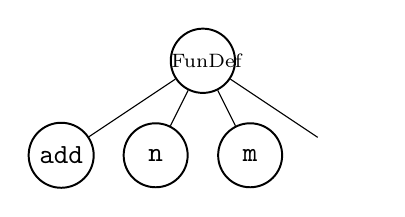
\begin{tikzpicture}[
    level distance=1.2cm,
    level 1/.style={sibling distance=1.2cm},
]
  \node [arn_u] {\scriptsize FunDef}
  child{
    node [arn_u] {\code{add}}
  }
  child{
    node [arn_u] {\code{n}}
  }
  child{
    node [arn_u] {\code{m}}
  }
  child{
    node [arn_w] {}
  };
\end{tikzpicture}
\end{center}

The root of the tree is the symbol FunDef, which explains that this tree
represents a function definition. The tree has four children: \code{add},
\code{n}, \code{m}, and the body expression. We do not know how to draw the tree
representing the body expression yet.

The body expression is an addition expression. It has two components: the
operands of the addition.

\begin{center}
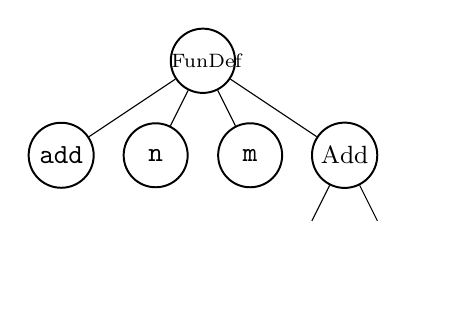
\begin{tikzpicture}[
    level distance=1.2cm,
    level 1/.style={sibling distance=1.2cm},
    level 2/.style={sibling distance=1.2cm}
]
  \node [arn_u] {\scriptsize FunDef}
  child{
    node [arn_u] {\code{add}}
  }
  child{
    node [arn_u] {\code{n}}
  }
  child{
    node [arn_u] {\code{m}}
  }
  child{
    node [arn_u] {\small Add}
    child{
      node [arn_w] {}
    }
    child{
      node [arn_w] {}
    }
  };
\end{tikzpicture}
\end{center}

The root of the tree is Add as the expression is addition. It has two
children: the operand expressions.

The first operand expression consists of a single component: \code{n}.

\begin{center}
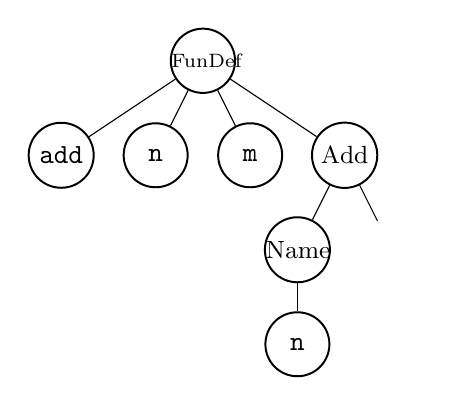
\begin{tikzpicture}[
    level distance=1.2cm,
    level 1/.style={sibling distance=1.2cm},
    level 2/.style={sibling distance=1.2cm}
]
  \node [arn_u] {\scriptsize FunDef}
  child{
    node [arn_u] {\code{add}}
  }
  child{
    node [arn_u] {\code{n}}
  }
  child{
    node [arn_u] {\code{m}}
  }
  child{
    node [arn_u] {\small Add}
    child{
      node [arn_u] {\small Name}
      child{
        node [arn_u] {\code{n}}
      }
    }
    child{
      node [arn_w] {}
    }
  };
\end{tikzpicture}
\end{center}

The root of the tree is Name, since the expression is just a name. The
only child is \code{n}.

The second operand expression can be similarly represented as a tree.

\begin{center}
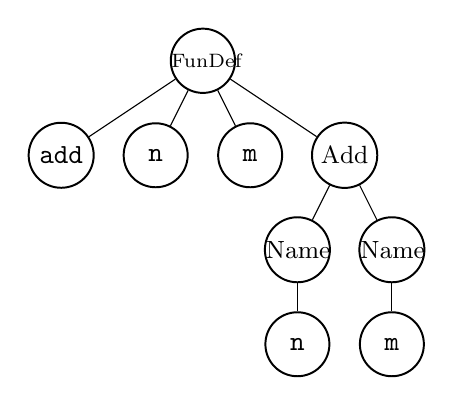
\begin{tikzpicture}[
    level distance=1.2cm,
    level 1/.style={sibling distance=1.2cm},
    level 2/.style={sibling distance=1.2cm}
]
  \node [arn_u] {\scriptsize FunDef}
  child{
    node [arn_u] {\code{add}}
  }
  child{
    node [arn_u] {\code{n}}
  }
  child{
    node [arn_u] {\code{m}}
  }
  child{
    node [arn_u] {\small Add}
    child{
      node [arn_u] {\small Name}
      child{
        node [arn_u] {\code{n}}
      }
    }
    child{
      node [arn_u] {\small Name}
      child{
        node [arn_u] {\code{m}}
      }
    }
  };
\end{tikzpicture}
\end{center}

The above tree represents the structure of the function definition. It is
independent of its underlying programming language. The tree can be a Python
function definition and a JavaScript function definition at the same time. By
expressing programs with trees, we can ignore unnecessary details in strings and
focus on the structures of programs.

As abstract syntax treats programs as trees, defining the abstract syntax of a
language is to define the set of every tree that represents a program. Let us
define the abstract syntax of \Lang. In \Lang, every natural number is a
program. A natural number program has only one component: the natural number
itself. Therefore, the following fact is true, where $E$ denotes the set of
every program:

\begin{center}
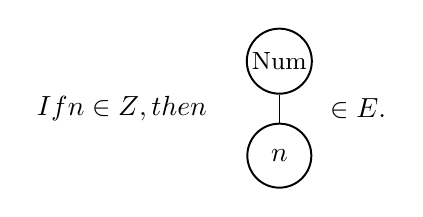
\begin{tikzpicture}[
    level distance=1.2cm,
    level 1/.style={sibling distance=1.2cm},
]
  \node at (-2,-0.6) {$\text{If }n\in\mathbb{Z}\text{, then}$};
  \node [arn_u] at (0,0) {\small Num}
  child{
    node [arn_u] {$n$}
  };
  \node at (1,-0.6) {$\in E$.};
\end{tikzpicture}
\end{center}

Addition of two arithmetic expressions is also a program. Such a program has
two components: the left and right operands. Each operand is an arithmetic
expression and thus a program. Therefore, the following fact is true:

\begin{center}
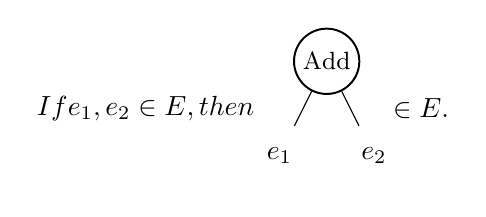
\begin{tikzpicture}[
    level distance=1.2cm,
    level 1/.style={sibling distance=1.2cm},
]
  \node at (-2.3,-0.6) {$\text{If }e_1,e_2\in E\text{, then}$};
  \node [arn_u] at (0,0) {\small Add}
  child{
    node [arn_nc] {$e_1$}
  }
  child{
    node [arn_nc] {$e_2$}
  };
  \node at (1.2,-0.6) {$\in E$.};
\end{tikzpicture}
\end{center}

Subtraction is similar.

\begin{center}
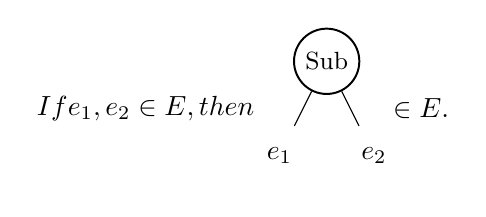
\begin{tikzpicture}[
    level distance=1.2cm,
    level 1/.style={sibling distance=1.2cm},
]
  \node at (-2.3,-0.6) {$\text{If }e_1,e_2\in E\text{, then}$};
  \node [arn_u] at (0,0) {\small Sub}
  child{
    node [arn_nc] {$e_1$}
  }
  child{
    node [arn_nc] {$e_2$}
  };
  \node at (1.2,-0.6) {$\in E$.};
\end{tikzpicture}
\end{center}

By collecting all the above facts, we can define the abstract syntax of \Lang as
the smallest set $E$ satisfying the following conditions.

\begin{center}
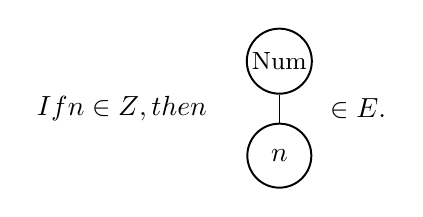
\begin{tikzpicture}[
    level distance=1.2cm,
    level 1/.style={sibling distance=1.2cm},
]
  \node at (-2,-0.6) {$\text{If }n\in\mathbb{Z}\text{, then}$};
  \node [arn_u] at (0,0) {\small Num}
  child{
    node [arn_u] {$n$}
  };
  \node at (1,-0.6) {$\in E$.};
\end{tikzpicture}
\end{center}

\begin{center}
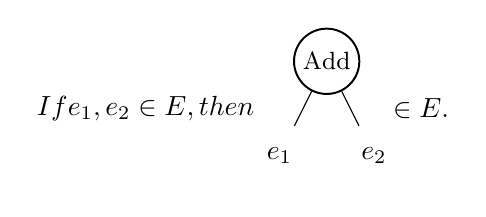
\begin{tikzpicture}[
    level distance=1.2cm,
    level 1/.style={sibling distance=1.2cm},
]
  \node at (-2.3,-0.6) {$\text{If }e_1,e_2\in E\text{, then}$};
  \node [arn_u] at (0,0) {\small Add}
  child{
    node [arn_nc] {$e_1$}
  }
  child{
    node [arn_nc] {$e_2$}
  };
  \node at (1.2,-0.6) {$\in E$.};
\end{tikzpicture}
\end{center}

\begin{center}
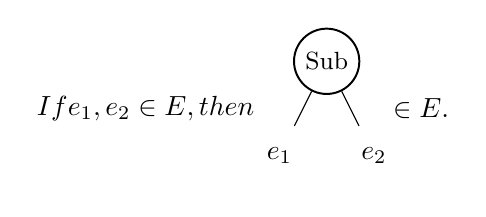
\begin{tikzpicture}[
    level distance=1.2cm,
    level 1/.style={sibling distance=1.2cm},
]
  \node at (-2.3,-0.6) {$\text{If }e_1,e_2\in E\text{, then}$};
  \node [arn_u] at (0,0) {\small Sub}
  child{
    node [arn_nc] {$e_1$}
  }
  child{
    node [arn_nc] {$e_2$}
  };
  \node at (1.2,-0.6) {$\in E$.};
\end{tikzpicture}
\end{center}

For example, the following tree represents an \Lang program:

\begin{center}
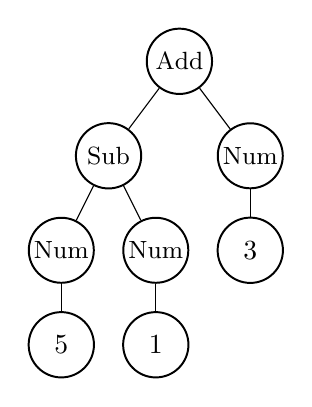
\begin{tikzpicture}[
    level distance=1.2cm,
    level 1/.style={sibling distance=1.8cm},
    level 2/.style={sibling distance=1.2cm},
]
  \node [arn_u] {\small Add}
  child{
    node [arn_u] {\small Sub}
    child{
      node [arn_u] {\small Num}
      child{
        node [arn_u] {$5$}
      }
    }
    child{
      node [arn_u] {\small Num}
      child{
        node [arn_u] {$1$}
      }
    }
  }
  child{
    node [arn_u] {\small Num}
    child{
      node [arn_u] {$3$}
    }
  };
\end{tikzpicture}
\end{center}

We call a tree that is an element of the set defined by abstract syntax an
\textit{abstract syntax tree}\index{abstract syntax tree} (\acrshort{astLabel}).

Abstract syntax can be easily implemented with ADTs in Scala. The following code
implements the abstract syntax of \Lang:

\begin{verbatim}
sealed trait AE
case class Num(value: Int) extends AE
case class Add(left: AE, right: AE) extends AE
case class Sub(left: AE, right: AE) extends AE
\end{verbatim}

\code{Num($n$)} corresponds to

\begin{center}
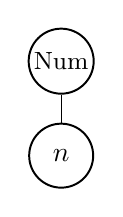
\begin{tikzpicture}[
    level distance=1.2cm,
    level 1/.style={sibling distance=1.2cm},
]
  \node [arn_u] {\small Num}
  child{
    node [arn_u] {$n$}
  };
\end{tikzpicture}
\end{center}

\code{Add($e_1$, $e_2$)} corresponds to

\begin{center}
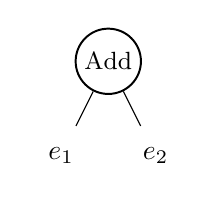
\begin{tikzpicture}[
    level distance=1.2cm,
    level 1/.style={sibling distance=1.2cm},
]
  \node [arn_u] {\small Add}
  child{
    node [arn_nc] {$e_1$}
  }
  child{
    node [arn_nc] {$e_2$}
  };
\end{tikzpicture}
\end{center}

\code{Sub($e_1$, $e_2$)} corresponds to

\begin{center}
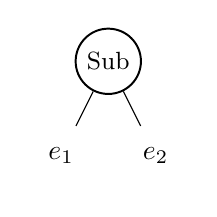
\begin{tikzpicture}[
    level distance=1.2cm,
    level 1/.style={sibling distance=1.2cm},
]
  \node [arn_u] {\small Sub}
  child{
    node [arn_nc] {$e_1$}
  }
  child{
    node [arn_nc] {$e_2$}
  };
\end{tikzpicture}
\end{center}

The previous AST can be written as \code{Add(Sub(Num(5),
Num(1)), Num(3))} in Scala.

It is inconvenient to draw a tree every time we need to express a program. For
this reason, people usually use notations that look like code to represent
trees. For example, we can simply write $n$ instead of drawing a tree whose root
is Num and only child is $n$ when it is clear that $n$ denotes an AST
from the context. Similarly, we can use $e_1+e_2$ and $e_1-e_2$
instead of trees that represent addition and subtraction, respectively. Note that
$+$ and $-$ in the notations are not the mathematical addition and subtraction
operators. They are just parts of the notations and do not have any meaning.

We can define the abstract syntax of \Lang again by using the above notations.
$E$ is the smallest set satisfying the following conditions:

\begin{itemize}
  \item If $n\in\mathbb{Z}$, then $n\in E$.
  \item If $e_1,e_2\in E$, then $e_1+e_2\in E$.
  \item If $e_1,e_2\in E$, then $e_1-e_2\in E$.
\end{itemize}

Even though the notations themselves do not look like trees at all, they still
represent ASTs. Also, symbols like $+$ and $-$ do not have any meaning. It
is extremely important to keep these points in your mind. Otherwise, you will
mix abstract syntax using notations up with concrete syntax in the end.

Notations are just notations. You can define different notations and use them.
For example, one may use $\embox{ADD}\ e_1\ e_2$ instead of $e_1 + e_2$ to represent
addition. You can freely choose notations, but once you define them, you should
consistently use them not to make other people confused.

To make the definition of abstract syntax more concise, we adopt BNF to the
definition of abstract syntax. We can re-define the abstract syntax of \Lang with
BNF:

\[e\ ::=\ n\ |\ e+e\ |\ e-e\]

We call each symbol that denotes a particular element in abstract syntax a
\textit{metavariable}.\index{metavariable}
It is called \textbf{meta}variable because it is a variable at a
meta-level, not the level of the defined programming language. For example, $e$
is a metavariable that ranges over programs, and $n$ is a metavariable that
ranges over integers.

We often use parentheses to express elements of abstract syntax without
ambiguity. For instance, $3-1+2$ can be interpreted in two ways:

\begin{center}
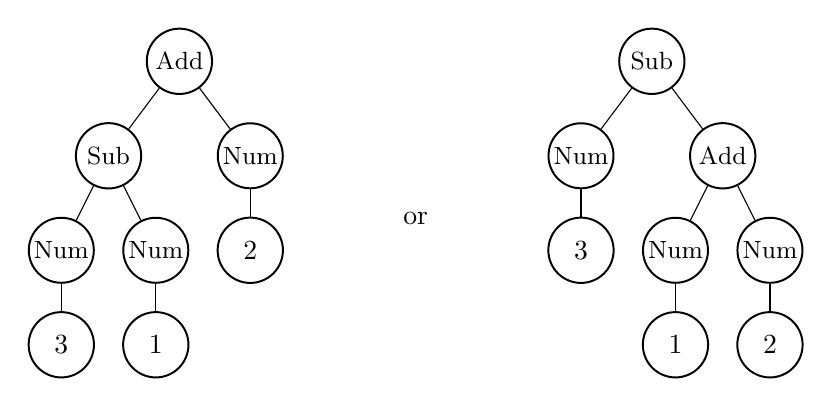
\begin{tikzpicture}[
    level distance=1.2cm,
    level 1/.style={sibling distance=1.8cm},
    level 2/.style={sibling distance=1.2cm},
]
  \node [arn_u] at (-3,0) {\small Add}
  child{
    node [arn_u] {\small Sub}
    child{
      node [arn_u] {\small Num}
      child{
        node [arn_u] {$3$}
      }
    }
    child{
      node [arn_u] {\small Num}
      child{
        node [arn_u] {$1$}
      }
    }
  }
  child{
    node [arn_u] {\small Num}
    child{
      node [arn_u] {$2$}
    }
  };
  \node at (0,-2) {or};
  \node [arn_u] at (3,0) {\small Sub}
  child{
    node [arn_u] {\small Num}
    child{
      node [arn_u] {$3$}
    }
  }
  child{
    node [arn_u] {\small Add}
    child{
      node [arn_u] {\small Num}
      child{
        node [arn_u] {$1$}
      }
    }
    child{
      node [arn_u] {\small Num}
      child{
        node [arn_u] {$2$}
      }
    }
  };
\end{tikzpicture}
\end{center}

If we write $(3-1)+2$, it is clear that it denotes the former. Otherwise, we
write $3-(1+2)$ to denote the latter.

\section{Parsing}

Concrete syntax considers programs as strings, while abstract syntax considers
programs as trees. Parsing bridges this gap. \textit{Parsing}\index{parsing} is
a process of transforming a string following concrete syntax into an AST. A
parser is a program that parses input. We can consider a parser as a partial
function from $S$ (the set of every string) to $E$ (the set of
every AST).

\[\embox{parse}: S\pto E\]

\begin{kaobox}[frametitle=Partial functions]
  A partial function from a set $A$ to a set $B$ is a function from a subset $S$ of
  $A$ to $B$. $S$ is called the domain of definition, or just domain in short, of the partial function.
  While $A\rightarrow B$ is a set of functions from $A$ to $B$, $A\pto B$ is a set
  of partial functions from $A$ to $B$.

  Let $f$ be a partial function from $A$ to $B$. Then, there can be $a\in A$ such
  that $f(a)$ is undefined. From a programmers' perspective, $f$ can be
  interpreted as a function from $A$ to \code{Option[$B$]}, where \code{None}
  means that the image is undefined and \code{Some($b$)} means that the image is
  $b$.
\end{kaobox}

The result of $\embox{parse}$
is undefined when an input does not belong to $P$ (the set of every
program). That is why $\embox{parse}$ is a partial function. When an input
belongs to $P$, $\embox{parse}$ results in its corresponding AST.

Consider the parser of \Lang. The results of $\embox{parse}$ are undefined for
the following strings as they are not \Lang programs:

\begin{itemize}
  \item \code{1+}
  \item \code{2*4}
  \item \code{0++3}
\end{itemize}

On the other hand, below is an example of when $\embox{parse}$ succeeds.

\begin{center}
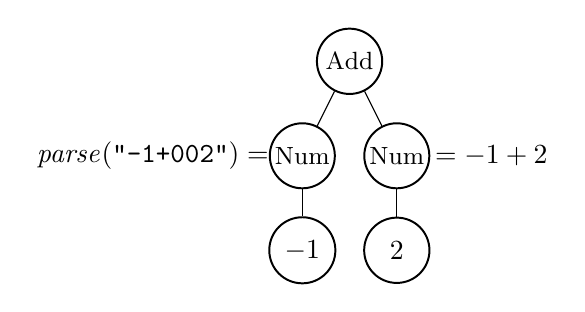
\begin{tikzpicture}[
    level distance=1.2cm,
    level 1/.style={sibling distance=1.2cm},
]
  \node at (-2.5,-1.2) {$\embox{parse}(\code{"-1+002"})=$};
  \node [arn_u] at (0,0) {\small Add}
  child{
    node [arn_u] {\small Num}
    child{
      node [arn_u] {$-1$}
    }
  }
  child{
    node [arn_u] {\small Num}
    child{
      node [arn_u] {$2$}
    }
  };
  \node at (1.8,-1.2) {$=-1+2$};
\end{tikzpicture}
\end{center}

This book does not discuss implementation of parsers.

\section{Semantics}

Syntax is an essential element of a programming language. It allows us to know
which strings are programs and what the structures of programs are. However,
syntax does not explain execution of programs. Programmers write programs to
execute them. They should know what will happen when their programs are
executed. Therefore, we need semantics in addition to syntax. Semantics is the
other essential element of a programming language. It defines the behaviors of
programs.

Let us define the semantics of \Lang. Semantics is defined based on abstract
syntax. The structure of a program determines its behavior. Since abstract
syntax represents the structure, it is natural to use abstract syntax for
semantics. The semantics of \Lang defines the semantics of each \Lang program,
where the semantics of a program means things that happen when the program is
executed. When an \Lang program is executed, it does one thing: outputs the
result of the evaluation of the arithmetic expression.
For example, $0+1$ should result
in $1$ if the semantics is defined correctly. Note that $+$ in $0+1$ does not
mean addition, and we cannot say anything about the result of $0+1$ until the
semantics is defined. To make \Lang a reasonable language, we must define the
semantics of \Lang so that $0+1$ results in $1$.

There are infinitely many programs. We cannot define the semantics of each
program separately. We need to utilize the structures of programs defined by the
abstract syntax. According to the abstract syntax, programs can split into three
groups: $n$, $e_1+e_2$, and $e_1-e_2$. By defining the semantics of each group
once, we can complete the semantics of infinitely many programs in a finite
method.

The simplest case is $n$. $n$ is an expression consisting of an integer. An
integer evaluates to itself. We represent this semantics as the following rule:

\semanticrule{Num}{
$n$ evaulates to $n$.
}

We can conclude the following facts by using Rule \textsc{Num}.

\begin{itemize}
  \item $1$ evaulates to $1$.
  \item $5$ evaulates to $5$.
\end{itemize}

The next case is $e_1+e_2$. As $e_1$ is an arithmetic expression, it results in
some integer. Let $n_1$ be the integer. Similarly, $e_2$ also results in some
integer. Let $n_2$ be the integer. Then, the result of $e_1+e_2$ is the sum of
$n_1$ and $n_2$. In this chapter, we use $\iadd$ instead of $+$ to denote
mathematical addition. It will help you distinguish mathematical addition from
$+$ used for the abstract syntax. Once you become familiar with syntax and
semantics, you can easily distinguish them by checking the context even if both
are denoted by $+$. From the next chapter, we will use $+$ for both abstract
syntax and mathematical addition. The following rule defines the semantics of
$e_1+e_2$.

\semanticrule{Add}{
If $e_1$ evaluates to $n_1$, and $e_2$ evaluates to $n_2$,\\
then $e_1+e_2$ evaluates to $n_1\iadd n_2$.
}

We can define the semantics of $e_1-e_2$ in a similar way. Like $\iadd$,
we use $\isub$ for mathematical subtraction in this chapter. The
following rule defines the semantics of $e_1-e_2$.

\semanticrule{Sub}{
If $e_1$ evaluates to $n_1$, and $e_2$ evaluates to $n_2$,\\
then $e_1-e_2$ evaluates to $n_1\isub n_2$.
}

These three rules are all of the semantics of \Lang. We now know the behavior of
every \Lang program. For example, consider $(3-1)+2$. The following steps
show why $(3-1)+2$ evaluates to $4$.

\begin{enumerate}
  \item (By Rule \textsc{Num}) $3$ evaluates to $3$.
  \item (By Rule \textsc{Num}) $1$ evaluates to $1$.
  \item (By Rule \textsc{Sub}) If $3$ evaluates to $3$ and $1$ evaluates to $1$, then $3-1$
    evaluates to $2$.
  \item (By 1, 2, and 3) $3-1$ evaluates to $2$.
  \item (By Rule \textsc{Num}) $2$ evaluates to $2$.
  \item (By Rule \textsc{Add}) If $3-1$ evaluates to $2$ and $2$ evaluates to $2$, then
    $(3-1)+2$ evaluates to $4$.
  \item (By 4, 5, and 6) $(3-1)+2$ evaluates to $4$.
\end{enumerate}

Now, let us define the semantics of \Lang in a more mathematical way. The
semantics defines the result of the execution of each program. Here, the result
is an integer. We can say that semantics outputs an integer when a program is
given. Thus, the semantics can be considered as a function from a program to an
integer.

\[\embox{eval}:E\rightarrow \mathbb{Z}\]

For each $e\in E$, there should exist a unique integer $\embox{eval}(e)$. It
is obviously true in \Lang. Every arithmetic expression evaluates to a unique
integer.

However, defining semantics as a function is a bad choice in other languages.
Some programs do not produce any results. Nonterminating programs are such
examples. Programs that incur run-time errors also belong to this category. You
will see programs with run-time errors in the next chapter. Moreover, there is a
program whose result is not unique. We call such programs nondeterministic
programs. For example, the behavior of a concurrent program with multiple
threads depends on how the threads are interleaved during execution. If the
threads are interleaved differently, the result may change. Programs without
results and nondeterministic programs prevent us from defining semantics as a
function. We should define semantics as a relation. Even though the semantics of
\Lang can be defined as a function, we define the semantics as a relation to
make the discussion of this chapter easily extendable to other languages.

We define the semantics of \Lang as $\Rightarrow$, a binary relation over $E$
and $\mathbb{Z}$.

\begin{kaobox}[frametitle=Binary relations]
A binary relation over sets $A$ and $B$ is a subset of $A\times B$,
where $A\times B=\{(a,b)\ |\ a\in A\land b\in B\}$.

Let $R$ be a binary relation over $A$ and $B$. Then, $R \subseteq A\times B$. For $a\in
A$ and $b\in B$, we write $a\ R\ b$ when $(a,b)\in R$. For example, $<$ is a
binary relation over $\mathbb{Z}$ and $\mathbb{Z}$, and we can write $1<2$ instead of
$(1,2)\in<$.
\end{kaobox}

\[\Rightarrow\subseteq E\times\mathbb{Z}\]

$(e,n)\in\Rightarrow$, i.e. $e\Rightarrow n$ implies that $e$ evaluates to $n$.

Let us define the semantics again with mathematical concepts.

\semanticrule{Num}{
$n\Rightarrow n$.
}

\vspace{-1em}

\semanticrule{Add}{
If $e_1\Rightarrow n_1$ and $e_2\Rightarrow n_2$,\\
then $e_1+e_2\Rightarrow n_1\iadd n_2$.
}

\vspace{-1em}

\semanticrule{Sub}{
If $e_1\Rightarrow n_1$ and $e_2\Rightarrow n_2$,\\
then $e_1-e_2\Rightarrow n_1\isub n_2$.
}

We use one more mathematical concept: inference rules. An \textit{inference
rule}\index{inference rule} is a rule to prove a new proposition from given
propositions. An inference rule has the following form:

\[
  \inferrule
  { \embox{premise}_1 \\ \embox{premise}_2 \\ \cdots \\ \embox{premise}_n }
  { \embox{conclusion} }
\]

It consists of a horizontal line, propositions above the line, and a proposition
below the line. We call the propositions above the line
\textit{premises}\index{premise} and the proposition below the line a
\textit{conclusion}\index{conclusion}. The rule means that if every premise is
true, then also the conclusion is true. A single inference rule can have zero or
more premises. A rule without premises implies that its conclusion is always
true. When a rule does not have any premises, we can omit the horizontal line.

Let us define the semantics of \Lang with inference rules.

\[
  n\Rightarrow n
  \quad\textsc{[Num]}
\]

\[
  \inferrule
  { e_1\Rightarrow n_1 \\ e_2\Rightarrow n_2 }
  { e_1+e_2\Rightarrow n_1\iadd n_2 }
  \quad\textsc{[Add]}
\]

\[
  \inferrule
  { e_1\Rightarrow n_1 \\ e_2\Rightarrow n_2 }
  { e_1-e_2\Rightarrow n_1\isub n_2 }
  \quad\textsc{[Sub]}
\]

As you can see, the rules are much clearer and more concise than the rules
written in a natural language.

We can prove $(3-1)+2\Rightarrow4$ with the rules. We usually draw a proof tree
when we prove a proposition with inference rules. A \textit{proof
tree}\index{proof tree} is a tree whose root is the proposition to be proven.
Each node of the tree is a proposition, and the children nodes of a node are
evidences supporting that the proposition of the node is true. Unlike most trees in
computer science, we place the root of a proof tree at the bottom. Every node is
placed below its children.

The following proof tree proves $3\Rightarrow3$.

\[3\Rightarrow3\]

The tree has only the root node because Rule \textsc{Num} does not have any
premises.

Similarly, the following proof tree proves $1\Rightarrow1$.

\[1\Rightarrow1\]

We draw the following proof tree with Rule \textsc{Sub} and the above trees
to prove $3-1\Rightarrow2$.

\[
  \inferrule
  { 3\Rightarrow3 \\ 1\Rightarrow1 }
  { 3-1\Rightarrow2 }
\]

By using Rule \textsc{Num} again, we prove $2\Rightarrow2$.

\[2\Rightarrow2\]

Finally, we get the proof tree of $(3-1)+2\Rightarrow4$.

\[
  \inferrule
  {
    \inferrule
    { 3\Rightarrow3 \\ 1\Rightarrow1 }
    { 3-1\Rightarrow2 }
    \\
    2\Rightarrow2
  }
  { (3-1)+2\Rightarrow4 }
\]

To explain what proof trees are, we have drawn the proof tree from its leaf
nodes. However, we usually draw a proof tree from the root node.
We start by drawing a horizontal line and writing the program we want to evaluate.

\[
  \inferrule
  {
    \color{white}
    \inferrule
    { 3\Rightarrow3 \\ 1\Rightarrow1 }
    { 3-1\Rightarrow2 }
    \\
    \color{white}
    2\Rightarrow2
  }
  { (3-1)+2\Rightarrow{\color{white}4} }
\]

Then, we find which inference rule can be applied. In this case, we can use Rule
\textsc{Add} since the program is addition.

\[
  \inferrule
  {
    \inferrule
    { \color{white}3\Rightarrow3 \\ \color{white}1\Rightarrow1 }
    { 3-1\Rightarrow\color{white}2 }
    \\
    2\Rightarrow\color{white}2
  }
  { (3-1)+2\Rightarrow{\color{white}4} }
\]

We need to evaluate $3-1$ and $2$ respectively. Let us focus on $3-1$ first.
Since $3-1$ is subtraction, we use Rule \textsc{Sub}.

\[
  \inferrule
  {
    \inferrule
    { 3\Rightarrow\color{white}3 \\ 1\Rightarrow\color{white}1 }
    { 3-1\Rightarrow\color{white}2 }
    \\
    2\Rightarrow\color{white}2
  }
  { (3-1)+2\Rightarrow{\color{white}4} }
\]

We can conclude that $3\Rightarrow3$ from Rule \textsc{Num}.

\[
  \inferrule
  {
    \inferrule
    { 3\Rightarrow3 \\ 1\Rightarrow\color{white}1 }
    { 3-1\Rightarrow\color{white}2 }
    \\
    2\Rightarrow\color{white}2
  }
  { (3-1)+2\Rightarrow{\color{white}4} }
\]

Similarly, $1\Rightarrow1$.

\[
  \inferrule
  {
    \inferrule
    { 3\Rightarrow3 \\ 1\Rightarrow1 }
    { 3-1\Rightarrow\color{white}2 }
    \\
    2\Rightarrow\color{white}2
  }
  { (3-1)+2\Rightarrow{\color{white}4} }
\]

By subtracting $1$ from $3$, we get $2$.

\[
  \inferrule
  {
    \inferrule
    { 3\Rightarrow3 \\ 1\Rightarrow1 }
    { 3-1\Rightarrow2 }
    \\
    2\Rightarrow\color{white}2
  }
  { (3-1)+2\Rightarrow{\color{white}4} }
\]

We use Rule \textsc{Num} again and get $2\Rightarrow2$.

\[
  \inferrule
  {
    \inferrule
    { 3\Rightarrow3 \\ 1\Rightarrow1 }
    { 3-1\Rightarrow2 }
    \\
    2\Rightarrow2
  }
  { (3-1)+2\Rightarrow{\color{white}4} }
\]

Finally, we can complete the proof tree and prove $(3-1)+2\Rightarrow4$.

\[
  \inferrule
  {
    \inferrule
    { 3\Rightarrow3 \\ 1\Rightarrow1 }
    { 3-1\Rightarrow2 }
    \\
    2\Rightarrow2
  }
  { (3-1)+2\Rightarrow4 }
\]

Sometimes, we call a proof tree proving the result of a program a
\textit{evaluation derivation}\index{evaluation derivation}
since the tree explains how the result of the program is derived.

The way of defining semantics we have seen so far is \textit{big-step
operational semantics}.\index{big-step operational semantics} It is called
``operational'' because it focuses on which \textbf{operation}s happen during execution
and ``big-step'' because it finds the result of a program by taking a single
\textbf{big} step. There are other ways to define semantics: denotational
semantics and small-step operational semantics. Most part of this book uses
big-step operational semantics. However, it will use small-step operational
semantics to deal with continuations later.

An \textit{interpreter}\index{interpreter} is a program that takes a program as
input and evaluates the program. We can easily implement an interpreter of
\Lang according to its semantics. The interpreter consists of a single function
that takes an AST as an argument and returns an integer.

\begin{verbatim}
def interp(e: AE): Int = e match {
  case Num(n) => n
  case Add(l, r) => interp(l) + interp(r)
  case Sub(l, r) => interp(l) - interp(r)
}
\end{verbatim}

\section{Syntactic Sugar}

\textit{Syntactic sugar}\index{syntactic sugar} adds a new feature to a language
by defining syntactic transformation rules instead of changing the semantics.
Syntactic sugar is widely used in real-world programming languages because it
allows languages to provide useful features without increasing the burden of the
language designers too much.

Suppose that we want to add integer negation to \Lang. It can be done by
modifying both syntax and semantics of \Lang. First, we fix the concrete syntax
to add integer negation.

\begin{verbatim}
<expr> ::= <number> | <expr> "+" <expr>
         | <expr> "-" <expr> | "-" "(" <expr> ")"
\end{verbatim}

Similarly, we fix the abstract syntax, too.

\[e\ ::=\ n\ |\ e+e\ |\ e-e\ |\ -e\]

The parser should be changed accordingly. For example, \code{-(03+4)} is parsed
to $-(3+4)$.

Finally, we add a new rule to the semantics to handle the $-e$ case.

\semanticrule{Neg}{
If $e$ evaluates to $n$,\\
then $-e$ evaluates to $\isub n$.
}

Note that $\isub$ denotes mathematical negation.

We can express the same thing as an inference rule.

\[
  \inferrule
  { e\Rightarrow n}
  { -e\Rightarrow\isub n }
  \quad\textsc{Neg}
\]

It requires considerable amount of work as we need to fix every component of the language.

Another way to add integer negation to \Lang is to add it as syntactic sugar. It
is enough to modify the concrete syntax and the parser. The change in the
concrete syntax is the same as before. Now, we fix the parser to parse \code{"-"
"(" expr ")"} to $0-e$ when \code{expr} is parsed to $e$. For example,
\code{-(03+4)} is parsed to $0-(3+4)$. Since $0\isub n=\isub n$ for any integer
$n$, we are done. It is the power of syntactic sugar. Language designers can
easily add new features by syntactically transforming them to existing features.
The procedure removing syntactic sugar by transformation is called
\textit{desugaring}\index{desugaring}.

We can find various examples of syntactic sugar in real-world languages. For
instance, for loops in Scala are supported as syntactic sugar.

\begin{quote}
  A for comprehension \code{for ($p$ <- $e$) yield $e'$} is translated to
  \code{$e$.map \{ case $p$ =>
  $e'$ \}}.\footnote{\url{https://www.scala-lang.org/files/archive/spec/2.13/06-expressions.html\#for-comprehensions-and-for-loops}}
\end{quote}

In addition, macros in languages like C, Scala, LISP, and Rust can be considered
as user-defined syntactic sugar.

\section{Exercises}

\begin{exercise}
\labex{syntax-and-semantics-expr}

Consider the following concrete syntax:

\begin{verbatim}
<expr> ::= <num>
         | "{" "+" <expr> <expr> "}"
         | "{" "*" <expr> <expr> "}"
         | "{" "let" "{" <id> <expr> "}" <expr> "}"
         | <id>
\end{verbatim}

Describe whether each of the following is \code{expr} and why.
\code{<id>} consists of one or more latin alphabets (\code{a-z}, \code{A-Z}), and
\code{<num>} consists of one or more digits (\code{0-9}).
Assume that it is allowed to add whitespaces among terminals freely.

\begin{enumerate}
  \item \verb!{let {x 5} {+ 8 {* x 2 3}}}!
  \item \verb!{with {x 0} {with {x 7}}}!
  \item \verb!{let {3 5} {+ 8 {- x 2}}}!
  \item \verb!{let {3 y} {+ 8 {* x 2}}}!
  \item \verb!{let {x y} {+ 8 {* x 2}}}!
\end{enumerate}

\end{exercise}

\begin{exercise}
\labex{syntax-and-semantics-icecream}

Consider the following concrete syntax:

\begin{verbatim}
<ice-cream> ::= "sprinkles" "on" <ice-cream>
              | "cherry" "on" <ice-cream>
              | "scoop" "of" <flavor> "on" <ice-cream>
              | "sugar-cone"
              | "waffle-cone"
<flavor>    ::= "vanilla"
              | "lettuce"
\end{verbatim}

Assume that it is allowed to add whitespaces among terminals freely.
Describe whether each of the following is \code{<ice-cream>} and why.

\begin{enumerate}
  \item \code{sprinkles}
  \item \code{sugar-cone}
  \item \code{vanilla}
  \item \code{scoop of vanilla on waffle-cone}
  \item \code{sprinkles on lettuce on waffle-cone}
  \item \code{scoop of vanilla on sprinkles on waffle-cone}
  \item \code{cherry on scoop of lettuce on scoop of vanilla on sugar-cone}
\end{enumerate}

\end{exercise}

\begin{exercise}
\labex{syntax-and-semantics-coffee}

Consider the following concrete syntax:

\newcommand{\BNF}[1]{\code{<#1>}}
\newcommand{\coffee}{\mbox{\BNF{coffee}}}
\newcommand{\milk}{\mbox{\BNF{milk}}}
\newcommand{\flavor}{\mbox{\BNF{flavor}}}

\[
\begin{array}{ccc}
  \code{espresso} \in \coffee
  &&
  \inferrule
  { e_1 \in \milk \\ e_2 \in \coffee }
  { e_1\ \code{"on"}\ e_2 \in \coffee }
  \\[2em]
  \inferrule
  { e_1 \in \coffee \\ e_2 \in \milk }
  { e_1\ \code{"on"}\ e_2 \in \coffee }
  &&
  \inferrule
  { e_1 \in \flavor \\ e_2 \in \coffee }
  { e_1\ \code{"on"}\ e_2 \in \coffee }
  \\[2em]
  \code{"milk-foam"} \in \milk
  &&
  \code{"steamed-milk"} \in \milk
  \\[2em]
  \code{"caramel"} \in \flavor
  &&
  \code{"cinnamon"} \in \flavor
  \\[2em]
  \code{"cocoa-powder"} \in \flavor
  &&
  \code{"chocolate-syrup"} \in \flavor
\end{array}
\]

Assume that it is allowed to add whitespaces among terminals freely.
Describe whether each of the following is \code{<coffee>} and why.

\begin{enumerate}
  \item \code{caramel latte macchiato}
  \item \code{espresso}
  \item \code{steamed-milk on caramel on milk-foam on espresso}
  \item \code{chocolate-syrup on cocoa-powder on cinnamon on milk-foam on steamed-milk on espresso}
  \item \code{steamed-milk on espresso on chocolate-syrup}
  \item \code{cocoa-powder on milk-foam on steamed-milk on espresso}
\end{enumerate}

\end{exercise}

\chapter{Identifiers}
\labch{identifiers}

\renewcommand{\plang}{\textsf{AE}\xspace}
\renewcommand{\Lang}{\textsf{VAE}\xspace}

Variables are one of the basic concepts of programming languages. A
\textit{variable}\index{variable} relates a name to a value. We use the
value of a variable by writing the name of the variable. For example, the following Scala program
prints \code{3}.

\begin{verbatim}
val x = 3
println(x)
\end{verbatim}

The program defines a variable whose name is \code{x} and value is \code{3}. At
the second line, the name \code{x} denotes the value \code{3}.

We call the names of variables identifiers. An
\textit{identifier}\index{identifier} is a name related to a
certain entity in a program. Not only the names of variables are identifiers;
there are various kinds of identifiers:

\begin{itemize}
\item Function names, which are related to functions
\item Parameter names, which are related to the values of arguments
\item Field names, which are related to values of fields
\item Method names, which are related to methods
\item Class names, which are related to classes
\end{itemize}

This chapter introduces identifiers. Identifiers in programs can split into
three groups: binding occurrences, bound occurrences, and free identifiers.
We will see what they are. This chapter discusses identifiers based on the use
of variables in programs. We will define \Lang by extending \plang of
\refch{syntax-and-semantics} with variables. Variables of \Lang are immutable.
We will deal with mutable variables in \refch{mutable-variables}.
In \Lang, the names of variables are
the only identifiers. However, as you have seen already, real-world programming
languages have many kinds of identifiers.

\section{Identifiers}

Identifiers name entities like variables and functions.
Let us discuss notions related to identifiers with the following Scala program:

\begin{verbatim}
f(0)
def f(x: Int): Int = {
  val y = 2
  x + y
}
f(1)
x - z
\end{verbatim}

In this program, \code{f}, \code{x}, \code{y}, and \code{z} are identifiers. Strictly speaking,
\code{Int} also is an identifier, but we ignore it because we do not want to take
types into account here.

A single identifier can occur multiple times in a program. For instance,
\code{f} occurs three times in the program: line 1, line 2, and line 6.
We can classify occurrences of identifiers into three categories:
binding occurrences, bound occurrences, and free identifiers.

An occurrence of an identifier is called a \textit{binding occurrence}\index{binding occurrence}
if the identifier occurs to be defined. A binding occurrence relates the
identifier to a particular entity. The program has three binding occurrences:

\begin{itemize}
  \item \code{f} at line 2

    It relates \code{f} to a function.

  \item \code{x} at line 2

    It relates \code{x} to the value of an argument given to \code{f}.

  \item \code{y} at line 3

    It relates \code{y} to the value \code{2}.
\end{itemize}

Every binding occurrence has its own scope. The \textit{scope}\index{scope} of a binding
occurrence means a code region where the indentifier defined by the binding
occurrence is alive, i.e. usable. The scope of each identifier in the program is as follows:

\begin{itemize}
  \item \code{f}

    A function can be used in its body (as Scala allows recursive function
    definitions) and at the lines below its definition. The scope of
    \code{f} is from line 3 to line 7.

  \item \code{x}

    A parameter of a function can be used only in the function body. The scope of
    \code{x} is line 3 and line 4.

  \item \code{y}

    A variable can be used at the lines below its definition. The scope of
    \code{y} is line 4.
\end{itemize}

An occurrence of an identifier is called a \textit{bound occurrence}\index{bound occurrence}
if the identifier occurs to use the entity related to itself. Since an
identifier becomes related to an entity by its binding occurrence, any bound
occurrences must reside in the scope of the binding occurrence.
The program has three bound occurrences:

\begin{itemize}
  \item \code{f} at line 6

    It denotes the function defined at line 2.

  \item \code{x} at line 4

    It denotes the value of an argument passed to \code{f}.

  \item \code{y} at line 4

    It denotes the value \code{2}.
\end{itemize}

An occurrence of an identifier is called a \textit{free identifier}\index{free
identifier} if it is
neither binding nor bound. A free identifier neither introduces a new name nor
uses a name defined already. It is not in the scope of any binding occurrence of
the same identifier. The program has three free identifiers:

\begin{itemize}
  \item \code{f} at line 1

    It is outside the scope of \code{f}.

  \item \code{x} at line 7

    It is outside the scope of \code{x}.

  \item \code{z} at line 7

    The program never defines \code{z}.
\end{itemize}

We call a free identifier a \textit{free variable}\index{free variable} when it
is the name of a variable. Therefore, both \code{x} and \code{z} at line 7 are
free variables.

Now, consider a binding occurrence that resides in the scope of a binding
occurrence of the same identifier. For example, the following program has two
binding occurrences of \code{x}, and the second binding occurrence is in the
scope of the first binding occurrence.

\begin{verbatim}
def f(x: Int): Int = {
  def g(x: Int): Int =
    x
  g(x)
}
\end{verbatim}

In this case, shadowing happens. \textit{Shadowing}\index{shadowing} means that
the innermost binding occurrence \textbf{shadow}s, i.e. temporarily invalidates,
the outer binding occurrences of the same name. Therefore, \code{x} at line 2
shadows \code{x} at line 1.
\code{x} at line 3 belongs to the scope of both binding occurrences simultaenously.
It denotes the value of an argument given to \code{g}, not \code{f}, because of
shadowing. On the other hand, \code{x} at line 4 denotes the value of an
argument given to \code{f} since it belongs to the scope of only \code{x} at
line 1.

\section{Syntax}

Let us define the abstract syntax of \Lang. We do not consider concrete
syntax anymore. Therefore, the term syntax will be used to mean abstract
syntax. Also, from now on, we use the term
\textit{expressions}\index{expression} rather than
programs when we discuss languages like \Lang. For example, we say that
$1+2$ is an expression of \plang, and $1$ and $2$ are the subexpressions of
$1+2$.

Recall the example at the beginning of the chapter:

\begin{verbatim}
val x = 3
println(x)
\end{verbatim}

To add variables to \plang, we need two kinds of expressions. The first kind is
expressions defining a variable, i.e. binding an identifier. In the example,
\code{val x = 3; println(x)} is such an expression. It defines the
variable \code{x} and starts the scope of \code{x} so that \code{x} can be used
in \code{println(x)}. We can conclude that an expression defining a variable
consists of three parts: the name of the variable, an expression determining the
value of the variable, and an expression that can use the variable. These parts
are \code{x}, \code{3}, and \code{println(x)}, respectively, in the example. The
second kind is expressions using a variable, i.e. a bound occurrence. In the
example, \code{x} at the second line is such an expression. It uses the variable \code{x} to denote
the value \code{3}. Based on this observation, we can define the syntax of
\Lang.

First, we need to add a new syntactic element: identifiers. The metavariable
$x$ ranges over identifiers. Let $\embox{Id}$ be the set of every
identifier.

\[x\in\embox{Id}\]

We do not care what $\embox{Id}$ really is.

The syntax of \Lang is as follows:\footnote{We omit the common part
to \plang.}

\[e\ ::=\ \cdots\ |\ \ebind{x}{e}{e}\ |\ x\]

\begin{itemize}
  \item $\ebind{x}{e_1}{e_2}$

    It defines a new variable whose name is $x$. Therefore, the occurrence of $x$ is a
    binding occurrence. $e_1$ decides the value denoted by the variable. The
    scope of the variable includes $e_2$ but excludes $e_1$.

  \item $x$

    It uses a variable; it is either a bound occurrence of $x$ or a free identifier.
    If it belongs to the scope of a binding occurrence of the same name, then it is a
    bound occurrence and denotes the value associated with the identifier.
    Otherwise, it is a free identifier, which denotes nothing.
\end{itemize}

\section{Semantics}

To define the semantics of \Lang, we need an additional semantic element that
stores the values denoted by variables. Without such an element, we cannot know the
value of each variable. We call the element an
\textit{environment}\index{environment}. An environment is a finite partial
function.\footnote{A finite partial function is a partial function whose domain
is a finite set.} The metavariable $\sigma$ ranges over environments.

\[\embox{Env}=\embox{Id}\finto\mathbb{Z}\]
\[\sigma\in\embox{Env}\]

For example, consider an environment $\sigma$.
If $\sigma(\cx)=1$, the value of a variable named \code{x} is $1$.
An environment is a partial function because it does not have the values
related to free identifiers. If a variable named \code{y} is free in
$\sigma$, then $\sigma(\cy)$ is undefined.
In addition, it is finite since every program
defines only finitely many identifiers.

Every expression in \Lang can evaluate to an integer only under some
environment. The reason is obvious: without environments, there is no way to
find the values of variables, and thus environments are essential to evaluation.

The following rule defines the semantics of $x$:

\semanticrule{Id}{
If
  $x$ is in the domain of $\sigma$,\\
then
  \evaldn{x}{\sigma(x)}.
}

If $x$ is an element of the domain of $\sigma$, $x$ is a bound occurrence. The
environment gives us the value denoted by $x$, which is $\sigma(x)$. Then, the
result is $\sigma(x)$. Otherwise, $x$ is not in the domain and is a free
identifier. In that case, we cannot evaluate $x$. The evaluation terminates
immediately. It can be interpreted as a run-time error.

Formally, the semantics of \Lang is a
ternary relation over $\embox{Env}$, $E$, and $\mathbb{Z}$ since it must take
environments into account.

\[\Rightarrow\subseteq\embox{Env}\times E\times\mathbb{Z}\]

$(\sigma,e,n)\in\Rightarrow$ is true if and only if
$e$ evaluates to $n$ under $\sigma$.
We write $\sigma\vdash e\Rightarrow n$ instead of $(\sigma,e,n)\in\Rightarrow$.
Intuitively, $\sigma$ and $e$ are inputs, and $n$ is the corresponding output.

Rule \textsc{Id} can be formulated as the following inference rule:
\footnote{$\dom{\sigma}$ denotes the domain of $\sigma$.}

\[
  \inferrule
  { x\in\dom{\sigma} }
  { \evald{x}{\sigma(x)} }
  \quad\textsc{[Id]}
\]

When a variable is defined, the value of the variable is added to the environment.
We write $\sigma[x\mapsto n]$ to denote an environment obtained by adding the
fact that $x$ denotes $n$ to $\sigma$. Then, the following property holds:

\[
\sigma [x\mapsto n](x') =
\begin{cases}
  n & \text{if}\ x=x' \\
  \sigma(x') & \text{if}\ x\neq x'
\end{cases}
\]

The following rule defines the semantics of $\ebind{x}{e_1}{e_2}$:

\semanticrule{Val}{
If
  \evaldn{e_1}{n_1}, and
  \evaln{\sigma[x\mapsto n_1]}{e_2}{n_2},\\
then
  \evaldn{\ebind{x}{e_1}{e_2}}{n_2}.
}

To evaluate $\ebind{x}{e_1}{e_2}$, we need to determine the value of $x$ first.
It can be done by evaluating $e_1$. Since the scope of $x$ excludes $e_1$,
the evaluation proceeds under $\sigma$, which is a given environment.
The result of $e_1$ is the value of $x$, and this information must be added to
the environment. By adding the fact to $\sigma$, we get $\sigma[x\mapsto n_1]$.
As $e_2$ is the scope of $x$, $e_2$ is evaluated under $\sigma[x\mapsto n_1]$.
The result of $e_2$ is the final result.

This semantics naturally explains shadowing. Let $x$ already be in the domain of
$\sigma$. Suppose that $\sigma(x)=n$. However, $e_2$ is evaluated under
$\sigma[x\mapsto n_1]$, and $\sigma[x\mapsto n_1](x)=n_1$. When $x$ is used in
$e_2$, its value is $n_1$, not $n$. Therefore, we can say that the
innermost definition of $x$ is used for the evaluation of $e_2$. This behavior
exactly matches the concept of shadowing explained before.

Rule \textsc{Val} can be expressed as the following inference rule:

\[
\inferrule
{
  \evald{e_1}{n_1} \\
  \eval{\sigma[x\mapsto n_1]}{e_2}{n_2}
}
{ \evald{\ebind{x}{e_1}{e_2}}{n_2} }
\quad\textsc{[Val]}
\]

The remaining cases are $n$, $\eadd{e_1}{e_2}$, and $\esub{e_1}{e_2}$.
Rules for those cases are basically identical to the rules of \plang.
However, we need to additionally take environments into account.

\semanticrule{Num}{
  \evaldn{n}{n}.
}

\vspace{-1em}

\semanticrule{Add}{
If
  \evaldn{e_1}{n_1}, and \evaldn{e_2}{n_2},\\
then
  \evaldn{\eadd{e_1}{e_2}}{n_1+n_2}.
}

\vspace{-1em}

\semanticrule{Sub}{
If
  \evaldn{e_1}{n_1}, and \evaldn{e_2}{n_2},\\
then
  \evaldn{\esub{e_1}{e_2}}{n_1-n_2}.
}

Integers, addition, and subtraction never update environments.
An integer evaluates to itself. Addition and subtraction evaluates their
subexpressions under the same environment.

We can express the rules in a natural language as the following inference rules:

\[
  \evald{n}{n}\quad\textsc{[Num]}
\]

\[
  \inferrule
  { \evald{e_1}{n_1} \\ \evald{e_2}{n_2} }
  { \evald{\eadd{e_1}{e_2}}{n_1+n_2} }
  \quad\textsc{[Add]}
\]

\[
  \inferrule
  { \evald{e_1}{n_1} \\ \evald{e_2}{n_2} }
  { \evald{\esub{e_1}{e_2}}{n_1-n_2} }
  \quad\textsc{[Sub]}
\]

The following proof tree proves that $\ebind{\cx}{1}{\eadd{\cx}{\cx}}$ evaluates
to $2$ under the empty environment. Note that $[x_1\mapsto n_1,\cdots,x_m\mapsto
n_m]$ denotes an environment whose domain includes from $x_1$ to $x_m$ and each
$x_i$ is mapped to $n_i$.

\[
\inferrule
{
  \emptyset\vdash 1\Rightarrow 1 \\
  \inferrule
  {
    \inferrule
    { \cx\in\dom{[ \cx\mapsto 1]} }
    { [ \cx\mapsto 1]\vdash \cx\Rightarrow 1 } \\
    \inferrule
    { \cx\in\dom{[ \cx\mapsto 1]} }
    { [ \cx\mapsto 1]\vdash \cx\Rightarrow 1 }
  }
  {[ \cx\mapsto 1]\vdash \eadd{\cx}{\cx}\Rightarrow 2 }
}
{ \emptyset\vdash \ebind{\cx}{1}{\eadd{\cx}{\cx}}\Rightarrow 2 }
\]

\section{Interpreter}

The following Scala code implements the abstract syntax of \Lang:

\begin{verbatim}
sealed trait Expr
case class Num(n: Int) extends Expr
case class Add(l: Expr, r: Expr) extends Expr
case class Sub(l: Expr, r: Expr) extends Expr
case class Val(x: String, i: Expr, b: Expr) extends Expr
case class Id(x: String) extends Expr
\end{verbatim}

An identifier is an arbitrary string.
\code{Val($x$, $e_1$, $e_2$)} corresponds to $\ebind{x}{e_1}{e_2}$;
\code{Id($x$)} corresponds to $x$.

We use a map to represent an environment. The type of an environment is
\code{Map[String, Int]}.

\begin{verbatim}
type Env = Map[String, Int]
\end{verbatim}

We can add a pair of a key and a value to a map with the \code{+} operator.
For example,
where \code{m} is \code{Map(1 -> "one")}, \code{m + (2 -> "two")} is the same as
\code{Map(1 -> "one", 2 -> "two")}.

\begin{verbatim}
def interp(e: Expr, env: Env): Int = e match {
  case Num(n) => n
  case Add(l, r) => interp(l, env) + interp(r, env)
  case Sub(l, r) => interp(l, env) - interp(r, env)
  case Val(x, i, b) => interp(b, env + (x -> interp(i, env)))
  case Id(x) => env(x)
}
\end{verbatim}

Since the structure of the code is almost identical to the semantics rules, there
is nothing much to explain. In the \code{Id} case, when \code{x} is a key in
\code{env}, the corresponding value becomes the result of \code{interp}.
Otherwise, an exception is thrown, and the execution
terminates without producing any results.

\section{Exercises}

\begin{exercise}
\labex{identifiers-arrow}

For each of the following expression:
\begin{itemize}
  \item $\ebind{\cx}{(\ebind{\cx}{3}{\esub{5}{\cx}})}{\eadd{1}{\cx}}$
  \item $\ebind{\cx}{3}{\ebind{\cy}{5}{\eadd{1}{\cx}}}$
  \item $\ebind{\cx}{3}{\ebind{\cx}{5}{\eadd{1}{\cx}}}$
\end{itemize}
\begin{enumerate}
  \item Draw arrows from each bound occurrence to its binding occurrence.
  \item Draw dotted arrows from each shadowing variable to its shadowed variable.
\end{enumerate}

\end{exercise}

\begin{exercise}
\labex{identifiers-shadowing-impl}

This exercise asks you to implement the \code{shadowing} function, which
takes a \Lang expression as an argument and returns the set of every
identifier that becomes shadowed at least once in the expression. For
example, \code{shadowing($e$)} equals \code{Set("x")} where $e$ denotes
$\ebind{\cx}{\cy}{\ebind{\cx}{1}{\cz}}$.  The \code{shadowing} function
calls the \code{helper} function, which tracks the set of every identifier
defined already to detect shadowing.

Complete the following implementation:

\begin{verbatim}
def shadowing(e: Expr): Set[String] = helper(e, Set())

def helper(e: Expr, env: Set[String]): Set[String] =
  e match {
    case Num(n) => ???
    case Add(l, r) => ???
    case Id(x) => ???
    case Val(x, e, b) => ???
  }
\end{verbatim}

\end{exercise}

\setchapterpreamble[u]{\margintoc}
\chapter{First-Order Functions}
\labch{first-order-functions}

The article defines F1VAE by adding \term{first-order functions} to VAE.
First-order functions cannot take functions as arguments or return functions. The
articles have followed the same pattern, extending a language by defining syntax
and semantics, since the previous one. This article and later articles omit
tedious details unless complex concepts appear.

F1VAE covered by the article differs from that of the lecture. The lecture
defines function definitions and expressions of F1VAE while the article
additionally defines programs of F1VAE. Defining programs makes the language
complete but is not the main topic of the article. Please focus on the syntax and
semantics of calling first-order functions.

\section{Syntax}

The following is the abstract syntax of F1VAE:

\[
\begin{array}{lrcl}
\text{Integer} & n & \in & \mathbb{Z} \\
\text{Variable} & x & \in & \textit{Id} \\
\text{Function Name} & f & \in & \textit{Id} \\
\text{Expression} & e & ::= & n \\
&& | & e + e \\
&& | & e - e \\
&& | & \textsf{val}\ x = e\ \textsf{in}\ e \\
&& | & x \\
&& | & f(e) \\
\text{Value} & v & ::= & n \\
\text{Function Definition} & d & ::= & f(x)=e \\
\text{Program} & P & ::= & e \\
&& | & d;P
\end{array}
\]

Expressions of F1VAE are function applications in addition to those of VAE.
\(f(e)\) is a function application, which applies a function named \(f\) to a
value denoted by \(e\).

The name, the name of a parameter, and a body expression defines a function.
Metavariable \(d\) and \(f\) respectively range over function definitions and
function names.

A program is either an expression or the pair of a function definition and a
program. In other words, it is an expression following an arbitrary number of
function definitions. Metavariable \(P\) ranges over programs.

The following is an example of an F1VAE program:

\[
\begin{array}{l}
id(x)=x; \\
twice(x)=x+x; \\
\textsf{val}\ x=1\ \textsf{in}\ twice(id(x))
\end{array}
\]

\section{Semantics}

\[
\begin{array}{lrcl}
\text{Environment} & \sigma & \in & \mathit{Id}\hookrightarrow \text{Value}
\end{array}
\]

An environment is a partial function from identifiers to values. It stores values
denoted by variables.

Evaluating an expression requires not only values denoted by variables but also
function definitions denoted by function names.

\[
\begin{array}{lrcl}
\text{Function Environment} & \Lambda & \in & \mathit{Id}\hookrightarrow
(\mathit{Id}\times\text{Expression})
\end{array}
\]

A function environment is a partial function from identifiers to pairs of
identifiers and expressions. It stores names of parameters and bodies denoted by
function names.

\[\Rightarrow\subseteq\text{Environment}\times\text{Function
Environment}\times\text{Expression}\times\text{Value}\]

An environment and a function environment are essential to evaluate an
expression. \(\Rightarrow\) is a relation over four sets. \(\sigma,\Lambda\vdash
e\Rightarrow v\) implies that evaluating \(e\) under \(\sigma\) and \(\Lambda\)
yields \(v\).

\[
\inferrule
{
  f\in\mathit{Domain}(\Lambda) \\
  \Lambda(f)=(x,e') \\
  \sigma,\Lambda\vdash e\Rightarrow v' \\
  \lbrack x\mapsto v'\rbrack,\Lambda\vdash e'\Rightarrow v
}
{ \sigma,\Lambda\vdash f(e)\Rightarrow v }
\]

The inference rule defines the semantics of a function application. An
environment used by a function body is an environment existing when the function
is defined but not called. Function definitions do not belong to the scopes of
the binding occurrences of any variables. Therefore, programs define every
function under the empty environment. The rule uses \(\lbrack x\mapsto
v'\rbrack\) instead of \(\sigma\lbrack x\mapsto v'\rbrack\) to evaluate \(e'\),
the body of a function. On the other hand, the scope of the binding occurrence of
every function name equals an entire program. A whole program is under the same
function environment. The rule uses \(\Lambda\) to evaluate both \(e\) and
\(e'\).

The other rules equal those of VAE except they need function environments.

\[
\sigma,\Lambda\vdash n\Rightarrow n
\]

\[
\inferrule
{ \sigma,\Lambda\vdash e_1\Rightarrow n_1 \\ \sigma,\Lambda\vdash
e_2\Rightarrow n_2 }
{ \sigma,\Lambda\vdash e_1+e_2\Rightarrow n_1+n_2 }
\]

\[
\inferrule
{ \sigma,\Lambda\vdash e_1\Rightarrow n_1 \\ \sigma,\Lambda\vdash
e_2\Rightarrow n_2 }
{ \sigma,\Lambda\vdash e_1-e_2\Rightarrow n_1-n_2 }
\]

\[
\inferrule
{
  \sigma,\Lambda\vdash e_1\Rightarrow v_1 \\
  \sigma\lbrack x\mapsto v_1\rbrack,\Lambda\vdash e_2\Rightarrow v_2
}
{ \sigma,\Lambda\vdash \textsf{val}\ x=e_1\ \textsf{in}\ e_2\Rightarrow v_2 }
\]

\[
\inferrule
{ x\in\mathit{Domain}(\sigma) }
{ \sigma,\Lambda\vdash x\Rightarrow \sigma(x)}
\]

The semantics of a program is a relation over function environments, programs,
and values. The semantics of an expression has already used \(\Rightarrow\), but
using \(\Rightarrow\) for also the semantics of a program retains clarity and
thus can be abused for convenience.

\[\Rightarrow\subseteq\text{Function
Environment}\times\text{Program}\times\text{Value}\]

\(\Lambda\vdash P\Rightarrow v\) implies that evaluating \(P\) under \(\Lambda\)
yields \(v\).

\[
\inferrule
{ \emptyset,\Lambda\vdash e\Rightarrow v }
{ \Lambda\vdash e\Rightarrow v }
\]

Evaluating a program without function definitions equals evaluating its
expression.

\[
\inferrule
{ \Lambda\lbrack f\mapsto(x,e)\rbrack\vdash P\Rightarrow v }
{ \Lambda\vdash f(x)=e;P\Rightarrow v }
\]

Evaluating a program that is the pair of a function definition and a program
equals evaluating the latter program under a function environment containing the
function definition.

\section{Implementing an Interpreter}

The following Scala code expresses the abstract syntax of F1VAE:

\begin{verbatim}
sealed trait Expr
case class Num(n: Int) extends Expr
case class Add(l: Expr, r: Expr) extends Expr
case class Sub(l: Expr, r: Expr) extends Expr
case class Val(x: String, i: Expr, b: Expr) extends Expr
case class Id(x: String) extends Expr
case class App(f: String, a: Expr) extends Expr
\end{verbatim}

Dictionaries encode both an environment and a function environment. The keys and
the values of an environment are strings and integers respectively. The keys and
the values of a function environment are strings and pairs of strings and
expressions of F1VAE respectively.

\begin{verbatim}
type Env = Map[String, Int]
type FEnv = Map[String, (String, Expr)]
\end{verbatim}

Function \verb!lookup! finds a value denoted by an identifier from an
environment. Function \verb!lookupFD! finds a function denoted by an identifier
from a function environment.

\begin{verbatim}
def lookup(x: String, env: Env): Int =
  env.getOrElse(x, throw new Exception)

def lookupFD(f: String, fEnv: FEnv): (String, Expr) =
  fEnv.getOrElse(f, throw new Exception)
\end{verbatim}

Function \verb!interp! takes an expression, an environment, and a function
environment as arguments and calculates a value denoted by the expression.

\begin{verbatim}
def interp(e: Expr, env: Env, fEnv: FEnv): Int = e match {
  case Num(n) => n
  case Add(l, r) => interp(l, env, fEnv) + interp(r, env, fEnv)
  case Sub(l, r) => interp(l, env, fEnv) - interp(r, env, fEnv)
  case Val(x, i, b) =>
    interp(b, env + (x -> interp(i, env, fEnv)), fEnv)
  case Id(x) => lookup(x, env)
  case App(f, a) =>
    val (x, e) = lookupFD(f, fEnv)
    interp(e, Map(x -> interp(a, env, fEnv)), fEnv)
}
\end{verbatim}

The \verb!App! case creates a new environment, which contains a single
identifier, to evaluate the body of a function.

The following is an example of calling \verb!interp!:

\begin{verbatim}
// id(x) = x;
// twice(x) = x + x;
// val x = 1 in twice(id(x))
interp(
  Val("x", Num(1),
    App("twice",
      App("id", Id("x"))
    )
  ),
  Map.empty,
  Map(
    "id" -> ("x", Id("x")),
    "twice" -> ("x", Add(Id("x"), Id("x")))
  )
)
// 2
\end{verbatim}

\section{Scope}

\subsection{Static Scope}

The semantics and the interpreter use \term{static scope}. Static scope enforces
function bodies to use environments existing when the functions are defined.
Calling below function \verb!f! always results in a run-time error.

\[f(x)=x+y\]

Static scope allows finding free identifiers and binding occurrences binding
bound occurrences without executing programs. Besides, every bound occurrence is
bound to a fixed single binding occurrence. Since code, not an execution,
determines entities referred by identifiers under static scope, \term{lexical
scope} is another name of static scope.

Most modern languages feature static scope.

\subsection{Dynamic Scope}

Unlike static scope, \term{dynamic scope} makes function bodies use environments
from function call-sites. A value denoted by identifier \(y\) of below function
\(f\) depends on a call-site. The identifier can be either free or bound.
Different binding occurrences may bind it during different calls.

\[f(x)=x+y\]

For example, the below expression denotes \(3\). At each call of \(f\), \(y\)
refers to a different value.

\[
\begin{array}{l}
f(x)=x+y; \\
(\textsf{val}\ y=1\ \textsf{in}\ f(0))\ +\ (\textsf{val}\ y=2\ \textsf{in}\ f(0))
\end{array}
\]

The following inference rule defines the semantics of a function application
using dynamic scope.

\[
\inferrule
{
  f\in\mathit{Domain}(\Lambda) \\
  \Lambda(f)=(x,e') \\
  \sigma,\Lambda\vdash e\Rightarrow v' \\
  \sigma\lbrack x\mapsto v'\rbrack,\Lambda\vdash e'\Rightarrow v
}
{ \sigma,\Lambda\vdash f(e)\Rightarrow v }
\]

Revising the \verb!App! case of the \verb!interp! function makes the interpreter
use dynamic scope.

\begin{verbatim}
def interp(e: Expr, env: Env, fEnv: FEnv): Int = e match {
  ...
  case App(f, a) =>
    val (x, e) = lookupFD(f, fEnv)
    interp(e, env + (x -> interp(a, env, fEnv)), fEnv)
}
\end{verbatim}

Dynamic scope prevents programs from being modular. An environment from a
call-site affects the behavior of a function under dynamic scope. Different parts
of a program unexpectedly interfere with each other. Programs show unexpected
behaviors and become error-prone.

Languages hardly feature dynamic scope. Common LISP is one example. \term{Macros}
in C behave similarly to functions under dynamic scope.

\begin{verbatim}
#define f(x) x + y

int main() {
    int y = 0;
    return f(0);
}
\end{verbatim}

\section{Exercises}

\begin{enumerate}
\item With the following list of function definitions in F1VAE:

\begin{tabular}{l}
\(\term{twice}(x) = x + x\) \\
\( x(y) = y\) \\
\( f(x) = x + 1\) \\
\( g(g) = g\)
\end{tabular}

Show the results of evaluating the following expressions under the empty environment.
When it is an error, describe which error it is.
\begin{itemize}
  \item[a)] \(\term{twice}\ \term{twice}\)

  \item[b)] \(\textsf{val}\ x=5\ \textsf{in}\ x\ x\)

  \item[c)] \(g\ 3\)

  \item[d)] \(g\ f\)

  \item[e)] \(g\ g\)
\end{itemize}

\item What are the results of the following expression:
\begin{verbatim}
{with {count {recfun {count n} {if0 n n {+ 1 {count {- n 1}}}}}}
      {with {count {fun {x} {+ 42 {count x}}}}
            {count 7}}}
\end{verbatim}

in different scoping semantics when we evaluate it under the following environment?
\begin{verbatim}
Map("count" -> CloV("y", Add(Num(13), Id("y")), Map()))
\end{verbatim}

\begin{itemize}
  \item[a)] Dynamic scope
  \item[b)] Static scope
\end{itemize}


\end{enumerate}

\setchapterpreamble[u]{\margintoc}
\chapter{First-Class Functions}
\labch{first-class-functions}

The article defines FAE by adding \term{first-class functions} to AE. First-class
functions are values: arguments for function calls and the return values of
functions. Functions taking functions as arguments or returning functions are not
first-order; they are \term{higher-order}. In most contexts, the terms
'first-class functions' and 'higher-order functions' are interchangeable.

\section{Syntax}

The following is the abstract syntax of FAE:

\[
\begin{array}{lrcl}
\text{Integer} & n & \in & \mathbb{Z} \\
\text{Variable} & x & \in & \textit{Id} \\
\text{Expression} & e & ::= & n \\
&& | & e + e \\
&& | & e - e \\
&& | & x \\
&& | & \lambda x.e \\
&& | & e\ e \\
\text{Value} & v & ::= & n \\
&& | & \langle \lambda x.e,\sigma \rangle \\
\text{Environment} & \sigma & \in & \textit{Id}\hookrightarrow\text{Value}
\end{array}
\]

An expression of FAE is an expression of AE, variable \(x\), \term{lambda
abstraction} \(\lambda x.e\), or \term{function application} \(e\ e\). A lambda
abstraction creates an anonymous function: \(\lambda x.e\) denotes a function
whose parameter and body are \(x\) and \(e\) respectively. \(x\) is a binding
occurrence. In function application \(e_1\ e_2\), \(e_1\) denotes a function, and
\(e_2\) denotes an argument. Evaluating a function application equals applying
its function to its argument.

A value of FAE is either an integer or a \term{closure}. A closure, which is a
function as a value, is the pair of a lambda abstraction and the environment of
when the lambda abstraction defines the function. Lambda abstractions may have
free identifiers, but the environments of closures store values denoted by the
free identifiers if a program is correct. Consider the following expression:

\[(\lambda x.\lambda y.x + y)\ 1\ 2\]

\(\lambda y.x+y\) contains free identifier \(x\). At run time, when the lambda
abstraction is evaluated, the environment of the moment knows that \(x\) refers
to \(1\). Hence, the environment of a closure defined by \(\lambda y.x+y\) also
knows that \(x\) refers to \(1\). The evaluation of the body of a closure happens
under the environment of the closure. \(x+y\) does not result in an error. The
next section shows the formal semantics of FAE and clarifies how lambda
abstractions and function applications operate.

An environment of FAE is a partial function from identifiers to values. Note that
values are not only integers but also closures.

\section{Semantics}

The semantics of FAE is a relation over environments, expressions, and values, as
that of VAE is.


\[\Rightarrow\subseteq\text{Environment}\times\text{Expression}\times\text{Value}\]

\(\sigma\vdash e\Rightarrow v\) implies that evaluating \(e\) under \(\sigma\)
yields \(v\).

The rules for integers, sums, differences, and variables equal those of VAE.

\[
\sigma\vdash n\Rightarrow n
\]

\[
\inferrule
{ \sigma\vdash e_1\Rightarrow n_1 \\ \sigma\vdash e_2\Rightarrow n_2 }
{ \sigma\vdash e_1+e_2\Rightarrow n_1+n_2 }
\]

\[
\inferrule
{ \sigma\vdash e_1\Rightarrow n_1 \\ \sigma\vdash e_2\Rightarrow n_2 }
{ \sigma\vdash e_1-e_2\Rightarrow n_1-n_2 }
\]

\[
\inferrule
{ x\in\mathit{Domain}(\sigma) }
{ \sigma\vdash x\Rightarrow \sigma(x)}
\]

A lambda abstraction creates a closure containing the current environment.

\[
\sigma\vdash \lambda x.e\Rightarrow \langle\lambda x.e,\sigma\rangle
\]

A function application evaluates its both subexpressions. Then, it evaluates the
body of the closure under an environment obtained by adding the value of the
argument to the environment of the closure.

\[
\inferrule
{ \sigma\vdash e_1\Rightarrow\langle\lambda x.e,\sigma'\rangle \\
  \sigma\vdash e_2\Rightarrow v' \\
  \sigma'\lbrack x\mapsto v'\rbrack\vdash e\Rightarrow v }
{ \sigma\vdash e_1\ e_2\Rightarrow v }
\]

The following proof tree proves that \((\lambda x.\lambda y.x+y)\ 1\ 2\) yields
\(3\).

\[
\inferrule
{
  \inferrule
  {
    \emptyset\vdash\lambda x.\lambda y.x+y\Rightarrow\langle\lambda x.\lambda
y.x+y,\emptyset\rangle \\
    \emptyset\vdash 1\Rightarrow 1 \\
    \lbrack x\mapsto 1\rbrack\vdash \lambda y.x+y\Rightarrow\langle\lambda
y.x+y,\lbrack x\mapsto 1\rbrack\rangle
  }
  { \emptyset\vdash(\lambda x.\lambda y.x+y)\ 1\Rightarrow\langle\lambda
y.x+y,\lbrack x\mapsto 1\rbrack\rangle } \\
  \emptyset\vdash2\Rightarrow 2 \\
  \inferrule
  {
    \inferrule
    { x\in\mathit{Domain}(\lbrack x\mapsto 1,y\mapsto 2\rbrack) }
    { \lbrack x\mapsto 1,y\mapsto 2\rbrack\vdash x\Rightarrow 1 } \\
    \inferrule
    { y\in\mathit{Domain}(\lbrack x\mapsto 1,y\mapsto 2\rbrack) }
    { \lbrack x\mapsto 1,y\mapsto 2\rbrack\vdash y\Rightarrow 2 }
  }
  { \lbrack x\mapsto 1,y\mapsto 2\rbrack\vdash x+y\Rightarrow 3 }
}
{ \emptyset\vdash(\lambda x.\lambda y.x+y)\ 1\ 2\Rightarrow 3 }
\]

\section{Implementing an Interpreter}

The following Scala code implements the abstract syntax and environments of FAE:

\begin{verbatim}
sealed trait Expr
case class Num(n: Int) extends Expr
case class Add(l: Expr, r: Expr) extends Expr
case class Sub(l: Expr, r: Expr) extends Expr
case class Id(x: String) extends Expr
case class Fun(x: String, b: Expr) extends Expr
case class App(f: Expr, a: Expr) extends Expr

sealed trait Value
case class NumV(n: Int) extends Value
case class CloV(p: String, b: Expr, e: Env) extends Value

type Env = Map[String, Value]
\end{verbatim}

Since a value is either an integer or a closure, \verb!Value!, instead of
\verb!Int!, denotes the type of values. The \verb!NumV! type corresponds to
integers; the \verb!CloV! type corresponds to closures. The type of environments
is a map from \verb!String! to \verb!Value!, but not \verb!Int!.

\begin{verbatim}
def lookup(x: String, env: Env): Value =
  env.getOrElse(x, throw new Exception)
\end{verbatim}

The \verb!lookup! function finds a value denoted by an identifier from an
environment.

\begin{verbatim}
def interp(e: Expr, env: Env): Value = e match {
  case Num(n) => NumV(n)
  case Add(l, r) =>
    val NumV(n) = interp(l, env)
    val NumV(m) = interp(r, env)
    NumV(n + m)
  case Sub(l, r) =>
    val NumV(n) = interp(l, env)
    val NumV(m) = interp(r, env)
    NumV(n - m)
  case Id(x) => lookup(x, env)
  case Fun(x, b) => CloV(x, b, env)
  case App(f, a) =>
    val CloV(x, b, fEnv) = interp(f, env)
    interp(b, fEnv + (x -> interp(a, env)))
}
\end{verbatim}

The \verb!Num! case creates a \verb!NumV! instance. Both \verb!Add! and
\verb!Sub! cases check whether values are integral, respectively calculate the
sum or the difference, and create \verb!NumV! instances. The \verb!Id! case
equals that of VAE. The \verb!Fun! case constructs a \verb!CloV! instance. The
\verb!App! case obtains a closure by evaluating the function, calculates the
argument, adds the argument to the environment of the closure, and evaluates the
body of the closure.

Passing \((\lambda x.\lambda y.x+y)\ 1\ 2\) and the empty environment to
\verb!interp! results in \verb!NumV(3)!.

\begin{verbatim}
// lambda x.lambda y.(x + y) 1 2
interp(
  App(
    App(
      Fun("x", Fun("y",
        Add(Id("x"), Id("y")))),
      Num(1)
    ),
    Num(2)
  ),
  Map.empty
)
// NumV(3)
\end{verbatim}

\section{Type Errors}

Free identifiers are the only reasons for run-time errors of VAE and F1VAE. On
the other hand, FAE expressions can result in run-time errors even though they do
not contain any free identifiers.

\[1 + \lambda x.x\]

The two premises of the inference rule for sums require both operands to denote
integers. The right operand of the above expression denotes a closure and thus
does not satisfy the premise. The expression does not yield any values;
interpreting the expressions causes a run-time error.

\[1\ 1\]

One of the premises of the inference rule for function applications enforces the
former subexpression of a function application to denote a closure. However,
\(1\) yields an integer, but not a closure. Like the previous one, the expression
does not yield any values and results in a run-time error.

Both expressions cause \term{type errors}. In the former, an expression denoting
a function occurs where an integer must come. In the latter, an expression
denoting an integer occurs where a function must come. Errors such as those from
the examples are type errors since their reasons are expressions of unexpected
types.

Syntactic methods can hardly prevent type errors. Such solutions restrict
languages too much. Consider restricting operands of sums and differences to only
integers rather than arbitrary expressions. Then, the syntax rejects many useful
or trivially correct expressions including \(1+1+1\). In the same manner,
restricting the first expressions of function applications to lambda abstractions
refuses \((\lambda x.\lambda y.x+y)\ 1\ 2\) and many others.

A \term{type system} is the most popular method to avoid type errors before
executions. Type systems prove that particular programs never cause type errors
at run time without executing them. Since they are the semantics of programs
before run time, \term{static semantics} is another name of them. To distinguish
'semantics,' whom the previous articles and the current article focus on, from
static semantics, \term{dynamic semantics} means 'semantics,' which defines the
run-time behaviors of programs. Type systems are out of the scope of the article,
and later articles discuss type systems in detail.

\section{Encoding VAE with FAE}

If one can transform every code of a language into code of another language
without changing its meaning, the latter can express everything the former
expresses. \term{Encoding} is rewriting a code written in a language with another
language.

VAE is encodable with FAE; FAE expresses everything VAE expresses; FAE is at
least as \term{expressive} as VAE. Precisely, FAE is more expressive than VAE.
The below \(\mathit{encode}\) function takes an expression of VAE as an argument
and returns an expression of FAE; it encodes VAE with FAE.

\[
\begin{array}{l}
\mathit{encode}(n)=n \\
\mathit{encode}(e_1+e_2)=\mathit{encode}(e_1)+\mathit{encode}(e_2) \\
\mathit{encode}(e_1-e_2)=\mathit{encode}(e_1)-\mathit{encode}(e_2) \\
\mathit{encode}(\textsf{val}\ x = e_1\ \textsf{in}\ e_2)=
\lambda x.\mathit{encode}(e_2)\ \mathit{encode}(e_1) \\
\mathit{encode}(x)=x
\end{array}
\]

Most cases are straightforward. The most important case is an expression
declaring a local variable. Hereafter, examples may declare local variables for
brevity even though they are written in languages without the feature. It is safe
to transform them to use lambda expressions and function applications.

Encoding complex languages with simple, but expressive languages can be
understood as desugaring code written in a language with various syntactic sugar.
Syntactic sugar provides convenience for programmers; desugaring provides
convenience for language designers: it simplifies implementations of interpreters
and compilers. Researchers often encode languages with others as well: encoding
makes proofs easier or allows borrowing already proven facts.

\term{Structural induction} proves the correctness of encodings. Such proofs are
beyond the scope of the article and the course.

\section{Exercises}

\begin{enumerate}
\item Given the following expression:

\[
\ebind{\cx}{5}{
    \ebind{\code{f}}{\efun{\cy}{\eadd{\cy}{\cx}}}{
        \eapp{(\efun{\code{g}}{\eapp{\code{f}}{(\eapp{\code{g}}{1})}})}
        {(\efun{\cx}{\cx})}
    }
}
\]
Describe a trace of the evalaution in terms of arguments to an \texttt{interp}
function for every call. (There will be 16 calls.) The \texttt{interp} function
takes two arguments --- an expression and a
   deferred substitution --- so show both for each call.  For number,
   variable, and \texttt{fun} expressions, show the result value, which
   is immediate. Use the back of the exam for additional space, and
   use the following abbreviations and possibly more abbreviations
 to save time:

\begin{center}
\begin{tabular}{lcl}
$E_0$ & = & the whole expression \\
$E_1$ & = & $\efun{\cy}{\eadd{\cy}{\cx}}$ \\
$E_2$ & = & $\efun{\code{g}}{\eapp{\code{f}}{(\eapp{\code{g}}{1})}}$ \\
$E_3$ & = & $\efun{\cx}{\cx}$ \\
$E_4$ & = & $\ebind{\code{f}}{E_1}{\eapp{E_2}{E_3}}$
\end{tabular}
\end{center}

\item In this exercise, we examine differences of semantics by changing scope.
The following code is an implementation of the interpreter for new language, AEF.
All the missing definitions are exactly the same as the ones for FAE.

\begin{verbatim}
def interp(e: Expr, env: Env): Value = e match {
  case Num(n) => NumV(n)
  case Add(l, r) =>
    val NumV(n) = interp(l, env)
    val NumV(m) = interp(r, env)
    NumV(n + m)
  case Sub(l, r) =>
    val NumV(n) = interp(l, env)
    val NumV(m) = interp(r, env)
    NumV(n - m)
  case Id(x) => lookup(x, env)
  case Fun(x, b) => CloV(x, b, env)
  case App(f, a) =>
    val CloV(x, b, fEnv) = interp(f, env)
    interp(b, __________ + (x -> interp(a, env)))
}
\end{verbatim}

Describe the semantics of the \texttt{App} case in AEF in prose
when we use each of the following for the blank above:
\begin{itemize}
  \item[a)] \texttt{env}
  \item[b)] \texttt{Map()}
  \item[c)] \texttt{fEnv}
\end{itemize}

\item In this exercise, we extend FAE to support multiple parameters. Consider the following language, MFAE:
\[
\begin{array}{lrll}
\text{Expression}& e ::= & n\\
&\mid& x\\
&\mid& \lambda x\ \cdots\ x. e\\
&\mid& e\ (e,\ \cdots ,\ e)\\
\text{Value}& v ::= & n \\
&\mid& \langle \lambda x \cdots\ x.e,\sigma \rangle \\
\end{array}
\]
where definition of $n,\ x,\ \sigma$ is same as FAE.
The semantics of some constructs are as follows:
\begin{itemize}
  \item Evaluating $\lambda x_1\ \cdots\ x_n. e$ under $\sigma$
      yields a closure $\langle \lambda x_1 \cdots\ x_n.e,\sigma \rangle$.
  \item If :
    \begin{itemize}
    \item Evaluating $e_0$ under $\sigma$ yields a closure $\langle \lambda x_1 \cdots\ x_n.e,\sigma' \rangle$
    \item Evaluating $e_i$ under $\sigma'$ yields $v_i$ for each $1 \leq i \leq n$
    \item Evaluating $e$ under $\sigma'[x_1 \mapsto v_1, \cdots, x_n \mapsto v_n]$ yields $v$
    \end{itemize}
\item[] then evaluating $e_0\ (e_1,\ \cdots ,\ e_n)$ under $\sigma$ yields $v$.
\end{itemize}

\begin{itemize}
  \item[a)] Write the operational semantics of the form \fbox{$\sigma\vdash e \Rightarrow v$} for the expressions.
  \item[b)] Write the evaluation derivation of the following expression:

\derive
{\hspace*{\textwidth}}
{\emptyset\vdash ($\lambda \code{f}\ \code{m}.\code{f}(\code{m})$)\
($\lambda \cx. \cx$,\ $8$) \Rightarrow~~~~~~~~}
\end{itemize}

\item Rewrite the following FVAE expression to FAE expression by extending ``encode`` function in section 9.5.
You should not ``evaluate'' them. (Consider $\code{if0}$ as an identifier.)

\begin{itemize}
    \item[a)] \(\textsf{val}\ \cx = \lambda \code{n}. \eadd{8}{\code{n}}\ \textsf{in}\ \lambda \code{n}. (\eapp{\cx}{(\esub{10}{\code{n}})}) \)
\item[b)] \(\textsf{val}\ \code{fac} = (\code{mk-rec}\
    (\lambda \code{fac}.\ \lambda \code{n}.\ (\code{if0}\ \code{n}\ 1 (\code{n} * (\code{fac}\ (\code{n} - 1))))))\ \textsf{in}\ (\code{fac}\ 10)\)
\item[c)] \(\lambda\ \code{body-proc}.\
\textsf{val}\ \code{fX} = \lambda\ \code{fX}.\
(\textsf{val}\ \code{f} = \lambda\ \cx.\ ((\code{fX}\ \code{fX})\ \cx)\
\textsf{in}\ (\code{body-proc}\ \code{f}))\
\textsf{in}\ (\code{fX}\ \code{fX}) \)
\end{itemize}

\item In this exercise, we extend FAE to check body expression when evaluating function expression.
Consider we extend value of FAE to include special value $\uparrow$ to represent error value at function body checking.
Write the operational semantics of the form
\fbox{$\sigma \vdash e \Rightarrow v$} for a function expression
$\lambda x. e$, when the semantics of the function expression
is changed as follows:
\begin{itemize}
\item If all free identifiers of $e$ is in $\sigma$ or is $x$, then evaluation of $\lambda x. e$ under $\sigma$ yields a closure
  contains function expression and the environment.
\item Otherwise, evaluation of $\lambda x. e$ under $\sigma$ yields a special value $\uparrow$.
\end{itemize}
You may use the function \textit{fv} which takes an
expression and returns a set of free identifiers in the expression.
For example, $fv(\lambda x. y\ x) = \{ y \}$.

\item In this exercise, we extend FAE to have record value. Consider the following language, RecFAE:
\[
\begin{array}{lrcl}
\text{Variable} & x & \in & \textit{Id} \\
\text{Field} & f & \in & \textit{Field} \\
\text{Record} & \rho & \in & \embox{Record} = \embox{Field} \finto \embox{Value} \\
\text{Expression}& e & ::= & x \\
&& \mid & \lambda x.e \\
&& \mid & e\ e \\
&& \mid & \{f\ e,\ \cdots,\ f\ e\}\\
&& \mid & e.f \\
&& \mid & e; e \\
&& \mid & (e) \\
\text{Value} & v & ::= & \rho \\
&& | & \langle \lambda x.e,\sigma \rangle \\
\end{array}
\]
where a value of the language is either a record $\rho$
or a closure $\langle\lambda x. e,\sigma\rangle$, and
an environment maps names to values:

The semantics of some constructs are as follows:
\begin{itemize}
  \item The evaluation of $\{f_1\ e_1,\ \cdots,\ f_k\ e_k\}$
    under $\sigma$ yields a finite map $\rho$,
which maps $f_i \in \{f_1\ \cdots,\ f_k\}$
to the value $v_i$ which is evaluated from the expression $e_i$ under $\sigma$.
  \item The evaluation of $e.f$ under $\sigma$ yields the value of the field $f$ in the record $\rho$,
      where evaluation $e$ under $\sigma$ yields \rho$.
  \item If evaluation of $e_1$ yields some value under $\sigma$, and evaluation of $e_2$ yields $v$ under same environment,
      then evaluation of $e_1; e_2$ yields $v$ under $\sigma$.
\item The evaluation of $(e)$ under any environment yields same value as evaluation of $e$.
\end{itemize}

Write the operational semantics of the form
$\boxed{\sigma \vdash e \Rightarrow v}$

\item In this exercise, we develop small language which only handles pair. Consider the following language Pair:
\[
\begin{array}{lrcl}
\text{Expression}& e & ::= & n \\
&&\mid& \verb!{pair ! e\ e\verb+}+\\
&&\mid& \verb!{first ! e\verb+}+\\
&&\mid& \verb!{second ! e\verb+}+\\
\text{Value} & v & ::= & \fbox{ (a) }
\end{array}
\]
where $n$ denotes a number and a value of the language is either a number or a pair of two values.
\begin{itemize}
  \item[a)] Write the grammar of the value $v$ and
 the operational semantics of the form \fbox{$\vdash e \Rightarrow v$} for the expressions.
  \item[b)] Write the evaluation derivation of the following expressions:

\hspace*{-5em}
 \derive
{\hspace*{\textwidth}}
{\vdash
 \{\texttt{second}\ \{\texttt{pair}\ 8\ \{
 \texttt{first}\ \{\texttt{pair}\ 320\ 42\}\}\}\}
 \Rightarrow~~~~~~~~}
\end{itemize}

\item In this exercise, we replace environment-baesd semantics of FVAE to subtitution-based semantics.
Consider the following language, FVAES:

\[
\begin{array}{lrcl}
\text{Expression} & e & ::= & n \\
&& | & \eadd{e}{e}\\
&& | & \esub{e}{e} \\
&& | & \ebind{x}{e}{e} \\
&& | & x \\
&& | & \efun{x}{e} \\
&& | & \eapp{e}{e} \\
\end{array}
\]

where evaluation of $e$ results in either a number $n$ or a closure $\efun{x}{e}$.

Consider the following implementation of FVAES:
\begin{verbatim}
trait FVAES
trait FVAESValue extends FVAES                                       // v ::= n | lambda x. e
case class Num(num: Int) extends FVAES with FVAESValue               // e ::= n
case class Add(left: FVAES, right: FVAES) extends FVAES              //     | e + e
case class Sub(left: FVAES, right: FVAES) extends FVAES              //     | e - e
case class Val(x: String, init: FVAES, body: FVAES) extends FVAES    //     | val x = e in e
case class Id(name: String) extends FVAES                            //     | x
case class Fun(x: String, body: FVAES) extends FVAES with FVAESValue //     | lambda x.e
case class App(fun: FVAES, arg: FVAES) extends FVAES                 //     | e e

// subst : (FVAES, String, FVAESValue) => FVAES
def subst(fvaes: FVAES, x: String, v: FVAESValue): FVAES = fvaes match {
  case Num(n) => fvaes
  case Add(l, r) => Add(subst(l, x, v), subst(r, x, v))
  case Sub(l, r) => Sub(subst(l, x, v), subst(r, x, v))
  case Val(y, i, b) => Val(y, subst(i, x, v), if (y == x) b else subst(b, x, v))
  case Id(name) => if (name == x) v else fvaes
  case Fun(y, b) => Fun(y, if (y == x) b else subst(b, x, v))
  case App(f, a) => App(subst(f, x, v), subst(a, x, v))
}

// interp : FVAES => FVAESValue
def interp(fvaes: FVAES): FVAESValue = fvaes match {
  case Num(n) => Num(n)
  case Add(l, r) => numAdd(interp(l), interp(r))
  case Sub(l, r) => numSub(interp(l), interp(r))
  case Val(x, i, b) => interp(subst(b, x, interp(i)))
  case Id(x) => error(s"free identifier: $x")
  case Fun(x, b) => Fun(x, b)
  case App(f, a) => interp(f) match {
    case Fun(x, b) => interp(subst(b, x, interp(a)))
    case fv => error(s"not a closure: $fv")
  }
}
\end{verbatim}

\begin{itemize}
  \item[a)]
Write the operational semantics of the above implementation 
of the form \fbox{$\vdash e \Rightarrow v$}
where $e[x/v]$ denotes \verb!subst(e, x, v)! and a value $v$ is either a number $n$ or
a closure $\efun{x}{e}$.

\begin{itemize}
  \item $e \equiv n$
  \item $e \equiv \eadd{e}{e}$
  \item $e \equiv \ebind{x}{e}{e}$
  \item $e \equiv \efun{x}{e}$
  \item $e \equiv \eapp{e}{e}$
\end{itemize}

  \item[b)] Write the definition of the substitution $e[x/v]$ denoting \verb!subst(e,x,v)!
of the form \fbox{$e[x/v] \leadsto e$}:
\begin{itemize}
  \item $e \equiv n$
%{\Large $n[x/v] \leadsto n$}
  \item $e \equiv \eadd{e}{e}$
  \item $e \equiv \ebind{x}{e}{e}$
  \item $e \equiv x$
  \item $e \equiv \efun{x}{e}$
  \item $e \equiv \eapp{e}{e}$
\end{itemize}

  \item[c)] Consider the following expression:

\[
\ebind{\code{z}}{\efun{\cx}{\esub{\cx}{\cy}}}{
    \ebind{\cy}{10}{
        (\eapp{\code{z}}{32})
    }
}
\]

\begin{itemize}
\item What is the result of evaluating the expression under the empty environment?
\item What is the result of evaluating the expression under the empty environment in FVAE?
\item Why are the results different?
\end{itemize}
    (Note: we can define equivalent semantics as FVAE using substitution
    by modifying \verb!subst! function)

%\verb!subst(With("y", Num(10), Id("z")), "z", Fun("x", Add(Id("x"), Id("y"))))!
%$[z/\verb!{fun {!z\verb!} {+ !x\ y\verb!}}!]\verb!{with {!y\ 10\verb!} !z\verb!}!$

\end{itemize}

\end{enumerate}

% \setchapterpreamble[u]{\margintoc}
\chapter{Lambda Calculus}
\labch{lambda-calculus}

\term{Lambda calculus} is a language featuring only variables, lambda
abstractions, and function applications. The article discusses how much lambda
calculus can express.

\section{Syntax}

The following is the abstract syntax of lambda calculus:

\[
\begin{array}{lrcl}
\text{Variable} & x & \in & \textit{Id} \\
\text{Expression} & e & ::= & x \\
&& | & \lambda x.e \\
&& | & e\ e \\
\text{Value} & v & ::= & \langle \lambda x.e,\sigma \rangle \\
\text{Environment} & \sigma & \in & \textit{Id}\hookrightarrow\text{Value}
\end{array}
\]

Unlike FAE, lambda calculus lacks integers, sums, and differences. An expression
is a variable, a lambda abstraction, or a function application. A value is a
closure but not an integer.

\section{Semantics}

The semantics of lambda calculus follows that of FAE.

\[\Rightarrow\subseteq\text{Environment}\times\text{Expression}\times\text{Value}\]

\[
\inferrule
{ x\in\mathit{Domain}(\sigma) }
{ \sigma\vdash x\Rightarrow \sigma(x)}
\]

\[
\sigma\vdash \lambda x.e\Rightarrow \langle\lambda x.e,\sigma\rangle
\]

\[
\inferrule
{ \sigma\vdash e_1\Rightarrow\langle\lambda x.e,\sigma'\rangle \\
  \sigma\vdash e_2\Rightarrow v' \\
  \sigma'\lbrack x\mapsto v'\rbrack\vdash e\Rightarrow v }
{ \sigma\vdash e_1\ e_2\Rightarrow v }
\]

\section{Church Numerals}

\term{Church numerals} encode numbers and operations treating number, such as
addition and multiplication, with lambda calculus. The following encode natural
numbers with lambda calculus:

\[
\begin{array}{rcl}
\mathit{encode}(0)&=&\lambda f.\lambda x.x \\
\mathit{encode}(1)&=&\lambda f.\lambda x.f\ x \\
\mathit{encode}(2)&=&\lambda f.\lambda x.f\ (f\ x) \\
\mathit{encode}(3)&=&\lambda f.\lambda x.f\ (f\ (f\ x)) \\
&\cdots&
\end{array}
\]

Intuitively, natural number \(n\) is a function that takes a function as an
argument and returns a function applying the argument \(n\) times:
\(\mathit{encode}(n)=f\mapsto f^n\). For any natural number \(n\) and any
function \(f\), \(n\ f\) equals \(f^n\).

The encoding of sums shows why the above encoding makes sense.

\[
\begin{array}{rcl}
+&\equiv&\lambda n.\lambda m.\lambda f.\lambda x.n\ f\ (m\ f\ x) \\
\mathit{encode}(e_1+e_2)&=&\lambda f.\lambda x.\mathit{encode}(e_1)\ f\
(\mathit{encode}(e_2)\ f\ x)
\end{array}
\]

For any natural number \(n\) and \(m\) and any function \(f\), \( (n+m)\ f\)
equals \(\lambda x.n\ f\ (m\ f\ x)\). Since \(n\ f\) equals \(f^n\), and \(m\ f\)
equals \(f^m\), it is \(\lambda x.f^n\ (f^m\ x)\) and equals \(\lambda x.f^{n+m}\
x\), or \(f^{n+m}\). Therefore, \(n+m\) equals \(f\mapsto f^{n+m}\), and the
\(\mathit{encode}\) function correctly encodes sums.

The following encodes products:

\[
\begin{array}{rcl}
\times&\equiv&\lambda n.\lambda m.\lambda f.\lambda x.n\ (m\ f)\ x \\
\mathit{encode}(e_1\times e_2)&=&\lambda f.\lambda x.\mathit{encode}(e_1)\
(\mathit{encode}(e_2)\ f)\ x
\end{array}
\]

For any natural number \(n\) and \(m\) and any function \(f\), \( (n\times m)\
f\) equals \(\lambda x.n\ (m\ f)\ x)\). Since \(m\ f\) equals \(f^m\), it is
\(\lambda x.n\ f^m\ x\). As \(n\ f\) is \(f^n\), \(n\ f^m\) is \( (f^m )^n\).
Hence, \(n\times m\) equals \(f\mapsto f^{n\times m}\), and the
\(\mathit{encode}\) function correctly encodes products.

Lambda calculus can encode differences and ratios as well. Moreover, it can
encode integers, rational numbers, and operations for them. They are beyond the
scope of the article.

\section{Church Booleans}

\term{Church Booleans} encode true, false, conditional expressions, logical sums,
logical products, and other logical language features. The hitherto defined
languages lack Boolean values. The section defines BAE by adding true, false, and
conditional expressions to AE.

\[
\begin{array}{lrcl}
\text{Boolean} & b & ::= & true \\
&& | & false \\
\text{Expression} & e & ::= & \cdots \\
&& | & b \\
&& | & \textsf{if}\ e\ e\ e \\
\text{Value} & v & ::= & \cdots \\
&& | & b
\end{array}
\]

It shows only features missed by AE. Metavariable \(b\) ranges over Boolean
values.

A conditional expression contains three subexpressions: the first one is its
condition; the second one is its true branch; the last one is its false branch.

\[
\vdash b\Rightarrow b
\]

\[
\inferrule
{ \vdash e_1\Rightarrow true \\ \vdash e_2\Rightarrow v }
{ \vdash \textsf{if}\ e_1\ e_2\ e_3\Rightarrow v}
\]

\[
\inferrule
{ \vdash e_1\Rightarrow false \\ \vdash e_3\Rightarrow v }
{ \vdash \textsf{if}\ e_1\ e_2\ e_3\Rightarrow v}
\]

If the condition of an expression is true, the true branch is evaluated, but the
false branch is not. Otherwise, the false branch is evaluated, but the true
branch is not.

The following encode true and false:

\[
\begin{array}{rcl}
\mathit{encode}(true)&=&\lambda a.\lambda b.a\ \_ \\
\mathit{encode}(false)&=&\lambda a.\lambda b.b\ \_ \\
\end{array}
\]

The underscore denotes an arbitrary expression. It implies that the value of an
argument is needless. It is possible to consider the underscore as any
expression, such as \(\lambda x.x\).

As the encoding of sums and products helps to understand the encoding of natural
number, the encoding of conditional expressions helps to understand the encoding
of true and false.

\[
\begin{array}{rcl}
\mathit{encode}(\textsf{if}\ e_1\ e_2\ e_3)&=&
\mathit{encode}(e_1)\ (\lambda\_ .\mathit{encode}(e_2))\ (\lambda\_
.\mathit{encode}(e_3))
\end{array}
\]

The underscore implies that a body does not refer to a parameter. Any parameter
name, such as \(x\), can replace the underscore. Assume that \(e_1\) denotes
true. The whole expression equals \( (\lambda a.\lambda b.a \_ )\ (\lambda\_
.\mathit{encode}(e_2))\ (\lambda\_ .\mathit{encode}(e_3))\), which is \(
(\lambda\_ .\mathit{encode}(e_2))\ \_ \). It denotes the same value as
\(\mathit{encode}(e_2)\) does. The evaluation of \(\mathit{encode}(e_3)\) is
unnecessary. If \(e_1\) denotes false, the expression denotes the same value as
\(\mathit{encode}(e_3)\) does, and the evaluation of \(\mathit{encode}(e_2)\) is
unnecessary.

Consider the following encoding:

\[
\begin{array}{rcl}
\mathit{encode}(true)&=&\lambda a.\lambda b.a \\
\mathit{encode}(false)&=&\lambda a.\lambda b.b \\
\textsf{if}&\equiv&\lambda c.\lambda a.\lambda b.c\ a\ b \\
\mathit{encode}(\textsf{if}\ e_1\ e_2\ e_3)&=&\mathit{encode}(e_1)\
\mathit{encode}(e_2)\ \mathit{encode}(e_3)
\end{array}
\]

It is simpler than the previous encoding but always evaluates both true and false
branches. Lambda calculus defined by the article uses eager evaluation, but
lambda calculus with lazy evaluation allows using the latter encoding without
computing needlessly. Later articles discuss lazy evaluation.

\section{Expressivity}

How expressive is lambda calculus? \term{Lambda computable} functions are
functions encodable with lambda calculus. Similarly, \term{Turing computable}
functions are functions implementable with \term{Turing machines}. Lambda
computable functions are Turing computable; Turing computable functions are
lambda computable. The set of every lambda computable function equals the set of
every Turing computable function; lambda calculus is \term{Turing complete}.
Computation doable with Turing machines almost equals that with real computers.
The only difference is that the tapes of Turing machines are infinite, while the
memories of computers are finite. Therefore, lambda calculus expresses everything
whom computers compute. Lambda calculus is 'the only' programming language.

\section{Exercises}

\setchapterpreamble[u]{\margintoc}
\chapter{Recursion}
\labch{recursion}

The article defines RFAE featuring recursive functions.

\section{CFAE}

CFAE adds conditional expressions to FAE.

\subsection{Syntax}

The below is the abstract syntax of CFAE. It shows a conditional expression,
which is the only new feature.

\[
\begin{array}{lrcl}
\text{Expression} & e & ::= & \cdots \\
&& | & \textsf{if0}\ e\ e\ e
\end{array}
\]

\(\textsf{if0}\) is similar to \(\textsf{if}\) of BAE, defined by the last
article, but its condition can be any value since CFAE lacks Boolean values. If a
condition is zero, the true branch is evaluated; otherwise, the false branch is
evaluated.

\subsection{Semantics}

The following define the semantics of conditional expressions:

\[
\inferrule
{ \sigma\vdash e_1\Rightarrow 0 \\ \sigma\vdash e_2\Rightarrow v }
{ \sigma\vdash \textsf{if0}\ e_1\ e_2\ e_3\Rightarrow v}
\]

\[
\inferrule
{ \sigma\vdash e_1\Rightarrow v' \\ v'\not=0 \\ \sigma\vdash e_3\Rightarrow v }
{ \sigma\vdash \textsf{if0}\ e_1\ e_2\ e_3\Rightarrow v}
\]

The semantics is similar to that of \(\textsf{if}\). Always one of the true and
false branches are evaluated, but not both.

\section{Recursion}

Is it possible to implement a factorial function with CFAE? Assume that CFAE
features multiplications. Firstly, consider a factorial function written
functionally. The following Scala function calculates factorials:

\begin{verbatim}
def factorial(n: Int): Int =
  if (n == 0) 1
  else n * factorial(n – 1)
\end{verbatim}

It seems the following CFAE expression is equivalent to the above code:

\[\textsf{val}\ factorial=\lambda n.\textsf{if0}\ n\ 1\ (n\times(factorial\
(n-1)))\ \textsf{in}\ \cdots\]

However, it is wrong since the scope of the binding occurrence of \(factorial\)
includes \(\cdots\) but excludes the lambda abstraction. Identifier \(factorial\)
in the lambda expression is free. CFAE disallows defining recursive functions.

\section{RFAE}

RFAE adds recursive functions to CFAE.

\subsection{Syntax}

The below is the abstract syntax of RFAE. It omits features common to CFAE.

\[
\begin{array}{lrcl}
\text{Expression} & e & ::= & \cdots \\
&& | & \textsf{def}\ x(x)=e\ \textsf{in}\ e
\end{array}
\]

\(\textsf{def}\ x_1(x_2)=e_1\ \textsf{in}\ e_2\) defines a recursive function. \(x_1\)
is the name of a function, and both \(e_1\) and \(e_2\) can refer to \(x_1\). For
example, the following is a factorial function:

\[\textsf{def}\ factorial(n)=\textsf{if0}\ n\ 1\ (n\times(factorial\ (n-1)))
\ \textsf{in}\ factorial\ 10\]

\subsection{Semantics}

The following defines the semantics of recursive functions:

\[
\inferrule
{ \sigma'=\sigma\lbrack x_1\mapsto\langle\lambda x_2.e_1,\sigma'\rangle\rbrack \\
  \sigma'\vdash e_2\Rightarrow v
}
{ \sigma\vdash \textsf{def}\ x_1(x_2)=e_1\ \textsf{in}\ e_2\Rightarrow v}
\]

The closure of a recursive function is similar to that of a lambda abstraction
but does not store the environment of the moment. Instead, it stores an
environment obtained by adding that the name of the function denotes the closure
to the environment. Calling a closure evaluates the body of the closure under the
environment of the closure so that recursive calls are valid.

The below proof trees prove that the factorial of one is one. The proof splits
into three trees for readability.

\[
\begin{array}{rcl}
\sigma_1&=&\lbrack f\mapsto\langle\lambda n.\textsf{if0}\ n\ 1\ (n\times(f\
(n-1))),\sigma_1\rangle\rbrack \\
\sigma_2&=&\sigma_1\lbrack n\mapsto 1\rbrack \\
&=&\lbrack f\mapsto\langle\lambda n.\textsf{if0}\ n\ 1\ (n\times(f\
(n-1))),\sigma_1\rangle,n\mapsto 1\rbrack \\
\sigma_3&=&\sigma_1\lbrack n\mapsto 0\rbrack \\
&=&\lbrack f\mapsto\langle\lambda n.\textsf{if0}\ n\ 1\ (n\times(f\
(n-1))),\sigma_1\rangle,n\mapsto 0\rbrack \\
\end{array}
\]

Assume the above.

\[
\inferrule
{
  \inferrule
  { f\in\mathit{Domain}(\sigma_2) }
  { \sigma_2\vdash f\Rightarrow \langle\lambda n.\textsf{if0}\ n\ 1\ (n\times(f\
(n-1))),\sigma_1\rangle }
  \\
  \inferrule
  {
    \inferrule
    { n\in\mathit{Domain}(\sigma_2) }
   { \sigma_2\vdash n\Rightarrow 1 } \\
    \sigma_2\vdash 1\Rightarrow 1
  }
  { \sigma_2\vdash n-1\Rightarrow 0 } \\
  \inferrule
  {
    \inferrule
    { n\in\mathit{Domain}(\sigma_3) }
    { \sigma_3\vdash n\Rightarrow 0 } \\
    \sigma_3\vdash 1\Rightarrow 1
  }
  { \sigma_3\vdash \textsf{if0}\ n\ 1\ (n\times(f\ (n-1))) \Rightarrow 1 }
}
{ \sigma_2\vdash f\ (n-1)\Rightarrow 1 }
\]

\[
\inferrule
{
  \inferrule
  { f\in\mathit{Domain}(\sigma_1)}
  { \sigma_1\vdash f\Rightarrow\langle\lambda n.\textsf{if0}\ n\ 1\ (n\times(f\
(n-1))),\sigma_1\rangle }
  \\
  {\sigma_1\vdash 1\Rightarrow 1}
  \\
  \inferrule
  {
    \inferrule
    { n\in\mathit{Domain}(\sigma_2) }
    { \sigma_2\vdash n\Rightarrow 1 } \\
    \inferrule
    {
      \inferrule
      { n\in\mathit{Domain}(\sigma_2) }
      { \sigma_2\vdash n\Rightarrow 1 } \\
      \sigma_2\vdash f\ (n-1)\Rightarrow 1
    }
    { \sigma_2\vdash (n\times(f\ (n-1)))\Rightarrow 1 }
  }
  {\sigma_2\vdash\textsf{if0}\ n\ 1\ (n\times(f\ (n-1)))\Rightarrow 1 }
}
{ \sigma_1\vdash f\ 1\Rightarrow 1 }
\]

\[
\inferrule
{
  \sigma_1=\lbrack f\mapsto\langle\lambda n.\textsf{if0}\ n\ 1\ (n\times(f\
(n-1))),\sigma_1\rangle\rbrack
  \\
  \sigma_1\vdash f\ 1\Rightarrow 1
}
{\emptyset\vdash
\textsf{def}\ f(n)=\textsf{if0}\ n\ 1\ (n\times(f\ (n-1)))\ \textsf{in}\ f\ 1
\Rightarrow 1
}
\]

\subsection{Implementing an Interpreter}

The following Scala code implements the abstract syntax and environments of RFAE:

\begin{verbatim}
sealed trait Expr
case class Num(n: Int) extends Expr
case class Add(l: Expr, r: Expr) extends Expr
case class Sub(l: Expr, r: Expr) extends Expr
case class Mul(l: Expr, r: Expr) extends Expr
case class Id(x: String) extends Expr
case class Fun(x: String, b: Expr) extends Expr
case class App(f: Expr, a: Expr) extends Expr
case class If0(c: Expr, t: Expr, f: Expr) extends Expr
case class Rec(f: String, x: String, b: Expr, e: Expr) extends Expr

sealed trait Value
case class NumV(n: Int) extends Value
case class CloV(p: String, b: Expr, var e: Env) extends Value

type Env = Map[String, Value]
def lookup(x: String, env: Env): Value =
  env.getOrElse(x, throw new Exception)
\end{verbatim}

\verb!If0! instnaces corresponds to conditional expressions; \verb!Rec! instances
corresponds to recursive functions. \verb!CloV! instances, which are closures,
have mutable environments because adding themselves to the environments requires
the environments mutable.

\begin{verbatim}
def interp(e: Expr, env: Env): Value = e match {
  case Num(n) => NumV(n)
  case Add(l, r) =>
    val NumV(n) = interp(l, env)
    val NumV(m) = interp(r, env)
    NumV(n + m)
  case Sub(l, r) =>
    val NumV(n) = interp(l, env)
    val NumV(m) = interp(r, env)
    NumV(n - m)
  case Mul(l, r) =>
    val NumV(n) = interp(l, env)
    val NumV(m) = interp(r, env)
    NumV(n * m)
  case Id(x) => lookup(x, env)
  case Fun(x, b) => CloV(x, b, env)
  case App(f, a) =>
    val CloV(x, b, fEnv) = interp(f, env)
    interp(b, fEnv + (x -> interp(a, env)))
  case If0(c, t, f) =>
    interp(
      if (interp(c, env) == NumV(0)) t else f,
      env
    )
  case Rec(f, x, b, e) =>
    val cloV = CloV(x, b, env)
    val nenv = env + (f -> cloV)
    cloV.e = nenv
    interp(e, nenv)
}
\end{verbatim}

The \verb!If0! case evaluates the true branch if the condition equals
\verb!NumV(0)! and the false branch otherwise. The \verb!Rec! case constructs a
closure and adds the closure to the environment of the closure.

The following calculates the factorial of three by calling the \verb!interp!
function:

\begin{verbatim}
// def f(n) = if0 n 1 (n * (f (n-1))) in f(3)
interp(
  Rec(
    "f", "n",
    If0(Id("n"),
        Num(1),
        Mul(
          Id("n"),
          App(Id("f"), Sub(Id("n"), Num(1)))
        )
    ),
    App(Id("f"), Num(3))
  ),
  Map.empty
)
// NumV(6)
\end{verbatim}

\section{Encoding Recursive Functions
}

As lambda calculus is Turing complete, recursive functions are encodable with
lambda calculus. Since both FAE and CFAE subsume the features of lambda calculus,
recursive functions are encodable with them as well.

\[
\begin{array}{rcl}
Z&\equiv&\lambda f.(\lambda x.f\ \lambda v.x\ x\ v)\ (\lambda x.f\ \lambda v.x\
x\ v)\\
\mathit{encode}(\textsf{def}\ x_1(x_2)=e_1\ \textsf{in}\ e_2)&=&
(\lambda x_1.e_2)\ (Z\ \lambda x_1.\lambda x_2.e_1)
\end{array}
\]

\(Z\) is a \term{fixed point combinator}; it calculates a fixed point of a given
function. A fixed point of a function is a value that makes the function yield
itself: a fixed point of function \(f\) is any \(x\) satisfying \(f(x)=x\). If an
argument given to \(Z\) is a function whose fixed point is a particular recursive
function, the result of applying \(Z\) to the function is the recursive function.
Consider \(\lambda f.\lambda x.\textsf{if0}\ x\ 1\ (x\times(f\ (x-1)))\). If
\(f\) is a factorial function, then \(\lambda x.\textsf{if0}\ x\ 1\ (x\times(f\
(x-1)))\) also is. Thus, the factorial function is a fixed point of \(\lambda
f.\lambda x.\textsf{if0}\ x\ 1\ (x\times(f\ (x-1)))\), and \(Z\ \lambda f.\lambda
x.\textsf{if0}\ x\ 1\ (x\times(f\ (x-1)))\) also is a factorial function.

How does the fixed point combinator work? \(Z\ \lambda f.\lambda x.\textsf{if0}\
x\ 1\ (x\times(f\ (x-1)))\) equals \( (\lambda x.f\ \lambda v.x\ x\ v)\ (\lambda
x.f\ \lambda v.x\ x\ v)\) if \(f\) denotes \(\lambda f.\lambda x.\textsf{if0}\ x\
1\ (x\times(f\ (x-1)))\). It equals \(f\ \lambda v.(\lambda x.f\ \lambda v.x\ x\
v)\ (\lambda x.f\ \lambda v.x\ x\ v)\ v\). Applying \(f\) to the argument results
in \(\lambda x.\textsf{if0}\ x\ 1\ (x\times(f\ (\lambda v.(\lambda x.f\ \lambda
v.x\ x\ v)\ (\lambda x.f\ \lambda v.x\ x\ v)\ v)\ (x-1)))\). Applying the
function to \(0\) yields \(1\) since \(x\) is \(0\). On the other hand, applying
the function to a nonzero value leads to \(x\times((\lambda v.(\lambda x.f\
\lambda v.x\ x\ v)\ (\lambda x.f\ \lambda v.x\ x\ v)\ v)\ (x-1))\). Then,
\(\lambda v.(\lambda x.f\ \lambda v.x\ x\ v)\ (\lambda x.f\ \lambda v.x\ x\ v)\
v\) has reappeared, but its argument has decreased by one. It successfully
simulates a recursive call and calculates factorials.

The following shows how to get the factorial of one:

\[
\begin{array}{rll}
& Z\ (\lambda f.\lambda x.\textsf{if0}\ x\ 1\ (x\times(f\ (x-1))))\ 1 \\
=&
(\lambda f.(\lambda x.f\ \lambda v.x\ x\ v)\ (\lambda x.f\ \lambda v.x\ x\ v))\
(\lambda f.\lambda x.\textsf{if0}\ x\ 1\ (x\times(f\ (x-1))))\ 1 \\
&& (f\leftarrow\lambda f.\lambda x.\textsf{if0}\ x\ 1\ (x\times(f\ (x-1)))) \\
\rightarrow &
(\lambda x.f\ \lambda v.x\ x\ v)\ (\lambda x.f\ \lambda v.x\ x\ v)\ 1 &
(f=\lambda f.\lambda x.\textsf{if0}\ x\ 1\ (x\times(f\ (x-1)))) \\
&& (x\leftarrow\lambda x.f\ \lambda v.x\ x\ v) \\
\rightarrow &
f\ (\lambda v.(\lambda x.f\ \lambda v.x\ x\ v)\ (\lambda x.f\ \lambda v.x\ x\ v)\
v)\ 1 \\
= &
(\lambda f.\lambda x.\textsf{if0}\ x\ 1\ (x\times(f\ (x-1))))\ (\lambda
v.(\lambda x.f\ \lambda v.x\ x\ v)\ (\lambda x.f\ \lambda v.x\ x\ v)\ v)\ 1\\
&& (f\leftarrow\lambda v.(\lambda x.f\ \lambda v.x\ x\ v)\ (\lambda x.f\ \lambda
v.x\ x\ v)\ v) \\
\rightarrow &
(\lambda x.\textsf{if0}\ x\ 1\ (x\times((\lambda v.(\lambda x.f\ \lambda v.x\ x\
v)\ (\lambda x.f\ \lambda v.x\ x\ v)\ v)\ (x-1))))\ 1 \\
&& (x\leftarrow 1) \\
\rightarrow &
1\times((\lambda v.(\lambda x.f\ \lambda v.x\ x\ v)\ (\lambda x.f\ \lambda v.x\
x\ v)\ v)\ 0)
\end{array}
\]

Via the fixed point combinator, a factorial function is implementable without
using a recursive function of RFAE.

\begin{verbatim}
// lambda f.(lambda x.f lambda v.x x v) (lambda x.f lambda v.x x v)
val Z =
  Fun("f",
    App(
      Fun("x",
        App(
          Id("f"),
          Fun("v", App(App(Id("x"), Id("x")), Id("v")))
        )
      ),
      Fun("x",
        App(
          Id("f"),
          Fun("v", App(App(Id("x"), Id("x")), Id("v")))
        )
      )
    )
  )

// (Z lambda f.lambda n.if0 n 1 (n * (f (n-1)))) 3
interp(
  App(
    App(
      Z,
      Fun("f", Fun("n",
        If0(Id("n"),
            Num(1),
            Mul(
              Id("n"),
              App(Id("f"), Sub(Id("n"), Num(1)))
            )
        )
      ))
    ),
    Num(3)
  ),
  Map.empty
)
// NumV(6)
\end{verbatim}

\section{Exercises}

\begin{enumerate}
\item Explain why the following code is an infinite loop and describe how to break the infinite loop:

\begin{verbatim}
 1 val mkRec = { bodyProc => {
 2   val fX = {fY => {
 3     val f = fY(fY)
 4     bodyProc(f)
 5   }};
 6   fX(fX)
 7 }};
 8 val fac = mkRec({ fac => {
 9   n => if0 (n) { 1 } else { (n * fac((n - 1))) }
10 }});
11 fac(10)
\end{verbatim}

\item Consider the following definition of \texttt{mkRec} and its use to define the recursive
function \texttt{fib}:

\begin{verbatim}
val mkRec = { bodyProc => {
  val fX = {fY => {
    val f = x => (fY(fY))(x)
    bodyProc(f)
  }};
  fX(fX)
}};
val fib = mkRec({ fib => {
  n => if ((n = 0) or (n = 1)) { 1 } else { (fib(n-1) + fib((n-2))) }
}});
fac(10)
\end{verbatim}

Describe what conditions \texttt{bodyProc} should satisfy so that \texttt{mkRec} can make its recursive version.

\item Let's call the following code $A$:
\begin{verbatim}
val fac = val facX = {facX => {
                       n => {
                         val fac = facX(facX);
                         if0 n 1 (n * fac(n-1))
                     }}};
          (facX facX);
fac(5)
\end{verbatim}
and the following code $B$:
\begin{verbatim}
val fac = val facX = {facX => {
                       val fac = facX(facX);
                       n => {
                         if0 n 1 (n * fac(n-1))
                       }}};
          (facX facX);
fac(5)
\end{verbatim}

\begin{itemize}
  \item[a)] What is the result of $A$?
  \item[b)] What is the result of $B$?
\end{itemize}

\item Write the value of \texttt{fac} at line 11:

\begin{verbatim}
 1 {with {fac
 2         {with {facX
 3                 {fun {facY}
 4                    {with {fac {fun {x} {{facY facY} x}}}
 5                          ; Exactly like original fac
 6                          {fun {n}
 7                             {if0 n
 8                                  1
 9                                  {* n {fac {- n 1}}}}}}}}
10               {facX facX}}}
11       {fac 10}}
\end{verbatim}

using the following Scala types:
\begin{verbatim}
trait FWAEValue
case class NumV(n: Int) extends FWAEValue
case class CloV(param: String, body: String, env: Env) extends FWAEValue
type Env = Map[String, FWAEValue]
\end{verbatim}
Note that the type of the body  of \texttt{CloV} is \texttt{String}.

\item Consider the following language $e$:
\[
\begin{array}{rll}
e ::= & n\\
\mid& \verb!{- ! e\ e\verb+}+\\
\mid& b\\
\mid& \verb!{and ! e\ e\verb+}+\\
\mid& \verb!{not ! e\verb+}+\\
\mid& \verb!{if ! e\ e\ e\verb+}+\\
\mid& x\\
\mid& \verb!{fun {! x^*\verb+} +e\verb+}+\\
\mid& \verb!{! e\ e^*\verb+}+\\
\mid& \verb!{rec {! x\ e\verb+} +e\verb+}+\\
\end{array}
\]
where $n$ denotes a number, $b$ denotes a boolean, $x$ denotes an identifier,
and a value $v$ of the language is one of a number, a boolean, or a closure
$\langle \lambda x_1\ \cdots\ x_n .\ e,\ \sigma\rangle$.
It does not support the short-circuiting semantics.
\begin{itemize}
  \item[a)]
Write the operational semantics of the form \fbox{$\sigma\vdash e \Rightarrow v$} for the expressions.
  \item[b)] Write the evaluation derivation of the following expressions:

\hspace*{-5em}
\derive {\hspace*{\textwidth}}
{\emptyset\vdash \{\{\texttt{fun}\ \{f\ m\}\ \{f\ m\}\}\
\{\texttt{fun}\ \{x\}\ x\}\ 8\} \Rightarrow~~~~~~~~}

% To Add
%%
\hspace*{-5em}
\derive
{\hspace*{\textwidth}}
{[\texttt{zero} \mapsto \langle 
\lambda x_1\ x_2\ x_3 .\ 
\texttt{\{if}\ x_1\ x_2\ x_3\texttt{\}},\
\emptyset\rangle] \vdash \term{pgm}
\Rightarrow~~~~~~~~
}

\bigskip
where \term{pgm} is as follows:
\[
\begin{array}{l}
\texttt{\{rec \{visit \{fun \{b\ n\} \{if b n \{visit \{not b\} \{zero n\}\}\}\}\}}\\
\texttt{\phantom{\{rec }\{rec \{zero \{fun \{x\} \{- 42 x\}\}\}}\\
\texttt{\phantom{\{rec \{rec }\{visit false 7\}\}\}}
\end{array}
\]

\end{itemize}


\end{enumerate}


\chapter{Boxes}
\labch{boxes}

\renewcommand{\plang}{\textsf{FAE}\xspace}
\renewcommand{\Lang}{\textsf{BFAE}\xspace}

Mutation is a widely-used feature. It is an important concept in imperative
languages. Even functional languages support mutation. Few languages are purely
functional, i.e. do not allow any mutation: e.g. Haskell and Coq. Mutation is
important since many programs can be implemented concisely and efficiently with
mutation. At the same time, mutation often makes programs difficult to be
reasoned about and error-prone. While binding of identifiers works modularly and
allows local reasoning, mutation has a global effect on execution and enables
uncontrolled interference between distinct parts of a program. Mutation should
be used with extreme care of programmers.

This chapter introduces mutation by defining \Lang, which extends \plang with
boxes. A \textit{box}\index{box} is a cell in memory that contains a single value. The value
contained in a box can be modified anytime after the creation of the box.
Boxes in \Lang are higher-order. Each box can contain any value, which can be
a box or a closure, rather than only an integer.
A box itself is rarely found in real-world languages: it is almost the same as
a reference in OCaml (\code{ref}). However, it is a good abstraction of more
general mutation mechanisms including mutable objects and data
structures. We can find such concepts in most languages, and boxes are useful to
understand those concepts.

We can consider mutable objects in Scala as generalization of boxes. By
going the opposite direction, we can say that boxes can be represented as
objects. Consider the following class definition in Scala:

\begin{verbatim}
case class Box(var value: Any)
\end{verbatim}

The class \code{Box} has one field: \code{value}. Like any other classes, we can
construct instances of \code{Box} and read the fields of the instances.

\begin{verbatim}
val b = Box(3)
println(b.value)
\end{verbatim}

It prints \code{3}.
In addition, since the field \code{value} is declared as mutable, we can mutate
its value.

\begin{verbatim}
b.value = 10
println(b.value)
\end{verbatim}

It changes the value of the field to \code{10} and prints \code{10}.

\section{Syntax}

The above Scala example shows three kinds of expressions regarding boxes:
creating a new box, reading the value of a box, and changing the value of a box.
To create a box, we need an expression that determines the initial value of the
box. To read the value of a box, we need an expression that determines the box.
To change the value of a box, we need an expression that determines the box and
an expression that determines the new value of the box.

In addition, there is another kind of expression that has been implicitly
used: the sequencing expression. Usually, an expression mutating a box is useless
per se. There should be other expressions that observe the change and do
other interesting things based on the change. To do so, we need to combine
multiple expressions to form a single expression. Such an expression
is the sequencing expression.

We can define the syntax of \Lang based on the observations.
The following is the syntax of \Lang:
\footnote{We omit the common part to \plang.}

\[
  e\ ::=\ \cdots\ |\ \eref{e}\ |\ \ederef{e}\ |\ \eset{e}{e}\ |\ \eseq{e}{e}
\]

\begin{itemize}
  \item $\eref{e}$

    It creates a new box, cf. \code{Box(3)} in the example.
    $e$ determines the initial value of the box.

  \item $\ederef{e}$

    It reads the value of a box, cf. \code{b.value} in the example.
    $e$ determines the box to be read.

  \item $\eset{e_1}{e_2}$

    It changes the value of a box, cf. \code{b.value = 10} in the example.
    $e_1$ determines the box to be updated; $e_2$ determines the new value.

  \item $\eseq{e_1}{e_2}$

    It is a sequencing expression. $e_1$ is the first expression to be
    evaluated; $e_2$ is the second. Many real-world languages allow sequencing
    of an arbitrary number of expressions. For brevity, \Lang allows only
    sequencing of two expressions. Sequencing of multiple expressions can be
    easily expresssed by nested sequencing. For example, $e_1;e_2;e_3$ can be
    expresssed as $(e_1;e_2);e_3$.
\end{itemize}

\section{Semantics}

Defining mutable memory is crucial to define the semantics of \Lang.
We call the memory of a program a \textit{store}\index{store}. A store records the values of boxes.
Each box is distinguished from another box by its address, i.e. every box has
its own address, which differs from the addresses of any other boxes.
The metavariable $a$ ranges over addresses. Let $\embox{Addr}$ be the set of every
possible address. We do not care about what $\embox{Addr}$ really is.

\[ a \in \embox{Addr} \]

A store is a finite partial function from addresses to values.
If the store maps an address $a$ to a value $v$, the value of the box whose
address is $a$ is $v$. The metavariable $M$ ranges over stores. Let $\embox{Sto}$
be the set of every store.

\[ \embox{Sto} = \embox{Addr}\finto V \]
\[ M \in \embox{Sto} \]

The semantics does not require a concrete notion of a box. Since every
box is uniquely identified by an address, the semantics can consider each
address as a box. Thus, we treat an address as a value of \Lang, instead of
introducing a new semantic element denoting boxes. For example, an expression
creating a box evaluates to an address. We need to revise the definition of a
value to include addresses.
\footnote{We omit the common part to \plang.}

\[ v\ ::=\ \cdots\ |\ a \]

Note that we keep using the concept of a box for explanation.
Even though the semantics abstracts boxes with addresses,
boxes do exist from the programmers' perspective.
The term box and the term address will be interchangeably used.

How are stores used in the semantics? First, consider an expression reading a
box. Evaluating \(\ederef{e}\) needs not only an environment but also a store.
If $e$ denotes a box, the store has the value of the box. The value becomes
the result of \(\ederef{e}\). Without a store, there is no way to find the value
of a box and yield a result. It implies that evaluation requires a store to be
given.

Now, let us consider the other kinds of expressions related to boxes.
$\eref{e}$ creates a new box; $\eset{e_1}{e_2}$ changes
the content of a box. Both modify stores. Modifying a store differs from
extending an environment with a new identifier.

A change in an environment is propagated to the subexpressions of an expression
that has caused the change. Consider $\ebind{x}{e_1}{e_2}$.
It extends the environment with $x$, but only $e_2$ uses the
extended environment because the scope of $x$ is $e_2$ but nowhere else.
A variable definition can affect only its subexpressions.
For instance, in $\eadd{(\ebind{x}{e_1}{e_2})}{e_3}$, $e_3$ does not belong to
the scope of $x$. The extended environment must be used for only $e_2$, but not
$e_3$. Therefore, we say that binding and environments are local and modular.

On the other hand, the modified store is unnecessary for the subexpressions of an
expression that modifies the store, while other parts of the program need
the modified one. Consider $\eseq{(\eset{\cx}{2})}{\ederef{\cx}}$ as an example.
Assume that $\cx$ denotes a box.
$\ederef{\cx}$ must be aware of that $\eset{\cx}{2}$ has changed the value of the box
to $2$. Otherwise, $\ederef{\cx}$ will get the previous value of the box and
produce a wrong result. Note that $\ederef{\cx}$ is not a subexpression of
$\eset{\cx}{2}$. However, in $\eset{\cx}{2}$, the evaluation of $2$, which is a
subexpression of $\eset{\cx}{2}$, must not be affected by the change in the value
of the box since the change happens after the evaluation of $2$. Therefore,
how stores change due to expressions is important. If an expression contains two
subexpressions, the store obtained by evaluating the first subexpression has to be
passed to the evaluation of the second subexpression. Stores are completely
different from environments. Any change in a store affects the entire remaining
computation. Stores are global and not modular.

From the observation, we can conclude that evaluation of an expression needs to
take a store in addition to an environment as input and output a new store along
with a result value. We can define the semantics as a
relation over $\embox{Env}$, $\embox{Sto}$, $E$, $V$, and $\embox{Sto}$.
The former store is input, and the latter store is output.

\[\Rightarrow\subseteq\embox{Env}\times\embox{Sto}\times E\times V\times\embox{Sto}\]

$\sevald{1}{e}{v}{2}$ is true if and only if \sevaldn{1}{e}{v}{2}.
We call this way of defining semantics a \textit{store-passing
style}\index{store-passing style}. The style allows defining \Lang, featuring
mutability, without any mutable concepts at the meta-level.

Now, let us define the semantics of each expression. We can easily reuse Rule
\textsc{Num}, Rule \textsc{Id}, and Rule \textsc{Fun} of \Lang by adding stores.
They maintain the contents of given stores.

\semanticrule{Num}{
  \sevaldn{}{n}{n}{}.
}

\vspace{-1em}

\[
  \sevald{}{n}{n}{}
  \quad\textsc{[Num]}
\]

\vspace{-1em}

\semanticrule{Id}{
  If $x$ is in the domain of $\sigma$,\\
  then \sevaldn{}{x}{\sigma(x)}{}.
}

\vspace{-1em}

\[
  \inferrule
  { x\in\dom{\sigma} }
  { \sevald{}{x}{\sigma(x)}{} }
  \quad\textsc{[Id]}
\]

\vspace{-1em}

\semanticrule{Fun}{
  \sevaldn{}{\efun{x}{e}}{\clov{x}{e}{\sigma}}{}.
}

\vspace{-1em}

\[
  \sevald{}{\efun{x}{e}}{\clov{x}{e}{\sigma}}{}
  \quad\textsc{[Fun]}
\]

During the evaluation of a certain expression,
the order of the evaluation among the subexpressions matters as they can modify the
store. Suppose that $x$ denotes a box, and the box contains $1$.
If the left operand of addition is evaluated before the right operand, in
$\eadd{(\eset{\cx}{2})}{\ederef{\cx}}$, $\ederef{\cx}$ evaluates to $2$ since it is
affected by the previous change. On the other hand, if the
right operand is evaluated first, $\ederef{\cx}$ evaluates to $1$ because
its evaluation precedes the modification and can observe only the original
value.

The order among the premises in a semantics rule does not specify the order of
evaluation. So far, we have not specified the order of evaluation in the
semantics as the order does not matter if there are no side
effects.\footnote{Side effects are any observable behaviors of expressions except the
results. Mutation and exceptions are side effects.}
 However, \Lang supports mutation, and we should specify
the order in the semantics. This goal can be naturally achieved by passing
stores. If we define the semantic to use the store that comes out from the
evaluation of the left operand as input of the evaluation of the right operand,
the order is determined to evaluate the left first.

A sequencing expression per se cannot modify a given store, but its subexpressions
can.

\semanticrule{Seq}{
  \begin{tabular}{@{\hskip0pt}l@{\hskip-10pt}l}
    If \\
    & \sevaldn{}{e_1}{v_1}{1}, and \\
    & \sevaldn{1}{e_2}{v_2}{2}, \\
    then \\
    & \sevaldn{}{\eseq{e_1}{e_2}}{v_2}{2}. \\
  \end{tabular}
}

\vspace{-1em}

\[
  \inferrule
  {
    \sevald{}{e_1}{v_1}{1} \\
    \sevald{1}{e_2}{v_2}{2} \\
  }
  { \sevald{}{\eseq{e_1}{e_2}}{v_2}{2} }
  \quad\textsc{[Seq]}
\]

$e_1$ is evaluated before $e_2$. The evaluation of $e_2$ must be aware of
any modifications of the store made by $e_1$.
For this purpose, the rule passes $M_1$, obtained by evaluating
$e_1$, to the evaluation of $e_2$. The result of $e_1$ is just discarded.
The final result is the same as the result of $e_2$.

Rule \textsc{Add}, Rule \textsc{Sub}, and Rule \textsc{App} are similar to
Rule \textsc{Seq}. They cannot modify stores, but their subexpressions can. The
evaluation order is the same as the sequencing expression. \Lang chooses
the left-to-right order for every expression, but other languages
may use a different order.

\semanticrule{Add}{
  \begin{tabular}{@{\hskip0pt}l@{\hskip-10pt}l}
    If \\
    & \sevaldn{}{e_1}{n_1}{1}, and \\
    & \sevaldn{1}{e_2}{n_2}{2}, \\
    then \\
    & \sevaldn{}{\eadd{e_1}{e_2}}{n_1+n_2}{2}.
  \end{tabular}
}

\vspace{-1em}

\[
  \inferrule
  {
    \sevald{}{e_1}{n_1}{1} \\
    \sevald{1}{e_2}{n_2}{2}
  }
  { \sevald{}{\eadd{e_1}{e_2}}{n_1+n_2}{2} }
  \quad\textsc{[Add]}
\]

\vspace{-1em}

\semanticrule{Sub}{
  \begin{tabular}{@{\hskip0pt}l@{\hskip-10pt}l}
    If \\
    & \sevaldn{}{e_1}{n_1}{1}, and \\
    & \sevaldn{1}{e_2}{n_2}{2}, \\
    then \\
    & \sevaldn{}{\esub{e_1}{e_2}}{n_1-n_2}{2}.
  \end{tabular}
}

\vspace{-1em}

\[
  \inferrule
  {
    \sevald{}{e_1}{n_1}{1} \\
    \sevald{1}{e_2}{n_2}{2}
  }
  { \sevald{}{\esub{e_1}{e_2}}{n_1-n_2}{2} }
  \quad\textsc{[Sub]}
\]

\vspace{-1em}

\semanticrule{App}{
  \begin{tabular}{@{\hskip0pt}l@{\hskip-10pt}l}
    If \\
    & \sevaldn{}{e_1}{\clov{x}{e}{\sigma'}}{1}, \\
    & \sevaldn{1}{e_2}{v'}{2}, and\\
    & \sevaln{\sigma'[x\mapsto v']}{M_2}{e}{v}{M_3}, \\
    then \\
    & \sevaldn{}{\eapp{e_1}{e_2}}{v}{3}.
  \end{tabular}
}

\vspace{-1em}

\[
  \inferrule
  {
    \sevald{}{e_1}{\clov{x}{e}{\sigma'}}{1} \\
    \sevald{1}{e_2}{v'}{2} \\
    \seval{\sigma'[x\mapsto v']}{M_2}{e}{v}{M_3}
  }
  { \sevald{}{\eapp{e_1}{e_2}}{v}{3} }
  \quad\textsc{[App]}
\]

Note that the evaluation of the body of a closure can modify the store as well.

Now, let us define the semantics of expressions treating boxes.
$\eref{e}$ is an expression creating a new box. The result of $e$ becomes the
initial value of the box. The result of $\eref{e}$ is the new box.

\semanticrule{NewBox}{
  \begin{tabular}{@{\hskip0pt}l@{\hskip-10pt}l}
    If \\
    & \sevaldn{}{e}{v}{1}, and \\
    & $a$ is not in the domain of $M_1$, \\
    then \\
    & \sevaln{\sigma}{M}{\eref{e}}{a}{M_1[a\mapsto v]}.
  \end{tabular}
}

\vspace{-1em}

\[
  \inferrule
  {
    \sevald{}{e}{v}{1} \\
    a\not\in \dom{M_1}
  }
  { \seval{\sigma}{M}{\eref{e}}{a}{M_1[a\mapsto v]} }
  \quad\textsc{[NewBox]}
\]

To get the initial value, $e$ is evaluated first. The address of the new
box must not belong to $M_1$, the store attained by evaluating $e$.
There is no additional condition the address must satisfy, so we can freely
choose any address that is not in $M_1$.
Note that if we check the domain of $M$, not $M_1$, we result in multiple
boxes sharing the same address, which is certainly wrong, when $e$ also creates
boxes.
The result is the address of the box. Also, we add a mapping from the address of
the box to the value of the box to the final store.

$\ederef{e}$ is an expression reading the value of a box. $e$ determines the box
to be read. If $e$ does not evaluate to a box, a run-time error occurs.
Otherwise, $e$ is some box, and the final result is the value of the box.

\semanticrule{OpenBox}{
  \begin{tabular}{@{\hskip0pt}l@{\hskip-10pt}l}
    If \\
    & \sevaldn{}{e}{a}{1}, and \\
    & $a$ is in the domain of $M_1$, \\
    then \\
    & \sevaln{\sigma}{M}{\ederef{e}}{M_1(a)}{M_1}.
  \end{tabular}
}

\vspace{-1em}

\[
  \inferrule
  {
    \sevald{}{e}{a}{1} \\
    a\in \dom{M_1}
  }
  { \seval{\sigma}{M}{\ederef{e}}{M_1(a)}{M_1} }
  \quad\textsc{[OpenBox]}
\]

To get a box, $e$ is evaluated. The result of $e$ must be an address that
belongs to $M_1$. The rule uses $M_1$ instead
of $M$ to find the value of the box. The reason is that $e$ can create a new
box and give the box as a result. Consider $\ederef{(\eref{1})}$. If the semantics
is correct, this expression must evaluate to $1$. The initial
store is empty, but evaluating $\eref{1}$ makes the store contain the address of
the box. It means that the address can be obtained only by looking into $M_1$,
not $M$. Therefore, the correct semantics uses $M_1$ to find the value of the
box.

$\eset{e_1}{e_2}$ is an expression changing the value of a box. $e_1$ determines the box
to be updated, and $e_2$ determines the new value of the box. Just like when we
open a box, $e_1$ must evaluate to a box. Otherwise, a run-time error will happen.

\semanticrule{SetBox}{
  \begin{tabular}{@{\hskip0pt}l@{\hskip-10pt}l}
    If \\
    & \sevaldn{}{e_1}{a}{1}, and \\
    & \sevaldn{1}{e_2}{v}{2}, \\
    then \\
    & \sevaln{\sigma}{M}{\eset{e_1}{e_2}}{v}{M_2[a\mapsto v]}.
  \end{tabular}
}

\vspace{-1em}

\[
  \inferrule
  {
    \sevald{}{e_1}{a}{1} \\
    \sevald{1}{e_2}{v}{2}
  }
  { \seval{\sigma}{M}{\eset{e_1}{e_2}}{v}{M_2[a\mapsto v]} }
  \quad\textsc{[SetBox]}
\]

Like all the other expressions, an expression modifying a box uses the left-to-right
order. If $e_1$ evaluates to an address $a$, the value associated with $a$ in
the store changes into the value denoted by $e_2$. Also, the value is the result
of the whole expression. This semantics follows the semantics of many real-world
imperative languages. For example, \code{x = 1} in C changes the value of
\code{x} to \code{1} and results in \code{1}. On the other hand, functional
languages usually use unit as the results of expressions for mutation. We can
easily adopt the semantics in \Lang by adding unit to the language.

\section{Interpreter}

The following Scala code implements the syntax of \Lang:
\footnote{We omit the common part to \plang.}

\begin{verbatim}
sealed trait Expr
...
case class NewBox(e: Expr) extends Expr
case class OpenBox(b: Expr) extends Expr
case class SetBox(b: Expr, e: Expr) extends Expr
case class Seqn(l: Expr, r: Expr) extends Expr
\end{verbatim}

\code{NewBox($e$)} represents $\eref{e}$;
\code{OpenBox($e$)} represents $\ederef{e}$;
\code{SetBox($e_1$, $e_2$)} represents $\eset{e_1}{e_2}$;
\code{Seqn($e_1$, $e_2$)} represents $\eseq{e_1}{e_2}$.

Addresses should be defined. We treat addresses as integers in Scala.

\begin{verbatim}
type Addr = Int
\end{verbatim}

In addition, we add a new variant of \code{Value} to represent boxes.
\footnote{We omit the common part to \plang.}

\begin{verbatim}
sealed trait Value
...
case class BoxV(a: Addr) extends Value
\end{verbatim}

\code{Box($a$)} represents $a$.

We use a map to represent a store. The type of a store is \code{Map[Addr, Value]}.

\begin{verbatim}
type Sto = Map[Addr, Value]
\end{verbatim}

\code{interp} takes an expression, an environment, and a store as arguments and
returns a pair of a value and a store.

\begin{verbatim}
def interp(e: Expr, env: Env, sto: Sto): (Value, Sto) =
  e match {
    ...
  }
\end{verbatim}

Let us see each case of the pattern matching.

\begin{verbatim}
case Num(n) => (NumV(n), sto)
case Id(x) => (env(x), sto)
case Fun(x, b) => (CloV(x, b, env), sto)
\end{verbatim}

The \code{Num}, \code{Id}, and \code{Fun} cases use given stores as the results.

\begin{verbatim}
case Seqn(l, r) =>
  val (_, ls) = interp(l, env, sto)
  interp(r, env, ls)
case Add(l, r) =>
  val (NumV(n), ls) = interp(l, env, sto)
  val (NumV(m), rs) = interp(r, env, ls)
  (NumV(n + m), rs)
case Sub(l, r) =>
  val (NumV(n), ls) = interp(l, env, sto)
  val (NumV(m), rs) = interp(r, env, ls)
  (NumV(n - m), rs)
case App(f, a) =>
  val (CloV(x, b, fEnv), ls) = interp(f, env, sto)
  val (v, rs) = interp(a, env, ls)
  interp(b, fEnv + (x -> v), rs)
\end{verbatim}

The \code{Seqn}, \code{Add}, \code{Sub}, and \code{App} cases do not directly
modify or read stores, but pass the stores returned from the recursive calls to the
next recursive calls or use them as results.

\begin{verbatim}
case NewBox(e) =>
  val (v, s) = interp(e, env, sto)
  val a = s.keys.maxOption.getOrElse(0) + 1
  (BoxV(a), s + (a -> v))
\end{verbatim}

The \code{NewBox} case computes the initial value of the box first. Then, it
computes an address not used in the store. We use the method \code{maxOption}.
If a collection is empty, the method returns \code{None}. Otherwise, the
result is \code{Some(n)}, where \code{n} is the greatest value in the collection.
By \code{.getOrElse(0)}, we can get \code{n} from \code{Some(n)} and \code{0}
from \code{None}. Consequently, \code{s.keys.maxOption.getOrElse(0)} results
in the maximum key in the store when the store is nonempty and \code{0}
otherwise. \code{a} is one greater than that value and thus does not belong to
the store. Therefore, we can use \code{a} as the address of the box.
The result of the function consists of the address and the extended store.

\begin{verbatim}
case OpenBox(e) =>
  val (BoxV(a), s) = interp(e, env, sto)
  (s(a), s)
\end{verbatim}

The \code{OpenBox} case evaluates the subexpression to get an address.
If the result is not a box, an exception is thrown due to a pattern matching
failure. The address is used to find the value of the box from the store.
The result of the function consists of the value of the box and the store from
the evaluation of the subexpression.

\begin{verbatim}
case SetBox(b, e) =>
  val (BoxV(a), bs) = interp(b, env, sto)
  val (v, es) = interp(e, env, bs)
  (v, es + (a -> v))
\end{verbatim}

The \code{SetBox} case evaluates both subexpressions and modifies the store.

\section{Exercises}

\begin{exercise}
\labex{mutable-boxes-trace}

Consider the following expression:
\[
  \eapp{(\efun{\cx}{\eapp{(\efun{\cy}{\eseq{\eset{\cx}{8}}{\ederef{\cy}}})}{\cx}})}{\eref{7}}
\]
Write the arguments and result of \code{interp} each time it is called
during the evaluation of the expression. Write them in the order in
which the calls to \code{interp} occur during evaluation.

\end{exercise}

\begin{exercise}
\labex{mutable-boxes-desugar}

This exercise asks you to implement the \code{desugar} function, which
takes a \Lang expression as an argument and returns an expression of the same
behavior without \textsf{;} (sequencing).

\begin{verbatim}
def desugar(e: Expr): Expr = e match {
  ...
  case Seqn(l, r) => ???
}
\end{verbatim}

Fill \code{???} to complete the implementation.
You may use the following helper functions without defining them:
\begin{verbatim}
// returns the set of every free identifier in e
def free(e: Expr): Set[String]

// returns a new identifier that does not belong to xs
def fresh(xs: Set[String]): String
\end{verbatim}

\end{exercise}

\begin{exercise}
\labex{mutable-boxes-landin}

We can implement a fixed point combinator with boxes. The key idea is to put a
dummy function in a box, create a recursive function with the box, and replace
the dummy function with the correct recursive function. This strategy is
known as \textit{Landin's knot}\index{Landin's knot}~\cite{landin1964mechanical}.

Complete the following implementation:

$\begin{array}{l}
  \ebind{\cz}{\efun{\cb}{(\\
  \ \ \ \ \ebind{\ca}{\eref{\efun{\cx}{\cy}}}{\\
  \ \ \ \ \ebind{\cf}{(\eapp{\cb}{???})}{\\
  \ \ \ \ \eseq{\eset{\ca}{???}}{\\
  \ \ \ \ ???\\
  }}})}}{\\
  \ebind{\cf}{\eapp{\cz}{(\efun{\cf}{\efun{\cv}{\sumbodyfv}})}}{\\
  \eapp{\cf}{10}}}
\end{array}$

\end{exercise}

\setchapterpreamble[u]{\margintoc}
\chapter{Mutable Variables}
\labch{mutable-variables}

\renewcommand{\plang}{\textsf{FAE}\xspace}
\newcommand{\bfae}{\textsf{BFAE}\xspace}
\renewcommand{\lang}{\textsf{MFAE}\xspace}

\bfae of the previous chatper provides boxes. Boxes are good abstraction
of mutable objects and data structures but do not explain mutable variables
well. Boxes, mutable objects, mutable data structures are values, while mutable
variables are names. Mutable variables allow the values associated with
names to change. We can find the notion of a mutable variable in many
real-world languages except a few functional languages including OCaml and
Haskell.

The semantics of mutable variables seem trivial. We can change the values of
mutable variables. However, if we use mutable variables with closures, we can do
many interesting things. Consider the following Scala program:

\begin{verbatim}
def makeCounter(): () => Int = {
  var x = 0
  def counter(): Int = {
    x += 1
    x
  }
  counter
}

val counter1 = makeCounter()
val counter2 = makeCounter()

println(counter1())
println(counter2())
println(counter1())
println(counter2())
\end{verbatim}

The program defines the function \code{makeCounter}. The function has a mutable
variable \code{x} whose initial value is \code{0}. Also, it defines and returns the function
\code{counter}. \code{counter} increases the value of \code{x} by
one every time it is called. We make two counters by calling \code{makeCounter}
twice. Then, we call each counter in turn and print the return value.
What does the program print? The first value will be \code{1} since
\code{counter1} will increase \code{x} by one from zero and return \code{x}.
However, predicting the other ones is difficult. We need the exact semantics of
mutable variables to answer the question.

This chapter defines \lang by extending \plang with mutable variables.
We will see the semantics of mutable variables. Addition of mutable
variables gives us a chance to explore a different design of the function
application semantics. We will see what is the call-by-reference semantics and how
it differs from the call-by-value semantics.

\section{Syntax}

As variables are mutable in \lang, we need to add expressions that change the
values of variables. The following is the abstract syntax of \lang:
\sidenote{We omit the common part to \plang.}

\[ e\ ::=\ \cdots\ |\ \eset{x}{e} \]

$\eset{x}{e}$ is an expression changing the value of a variable. $x$ is the
variable to be updated; $e$ determines the new value of the variable. Unlike
$\eset{e_1}{e_2}$ in \bfae, the left-hand-side of an assignment is restricted to
a variable. The reason is that variables are not values. We cannot get a
variable by evaluating an expression. The only way to designate a variable is
to write the name of the variable, and the syntax reflects this point.

Note that \lang lacks sequencing expressions, which exist in \bfae. Actually, it
is not problematic at all. We can desugar sequencing expressions into
lambda abstractions and function applications: transform $\eseq{e_1}{e_2}$ into
$\eapp{(\efun{x}{e_2})}{e_1}$, where $x$ is not free in $e_2$. The semantics of
$\eseq{e_1}{e_2}$ is that evaluating $e_1$ first and then $e_2$. The evaluation
of $\eapp{(\efun{x}{e_2})}{e_1}$ is the same. First, $\efun{x}{e_2}$ evaluates
to a closure, which means that $e_2$ is not evaluated. Then, the argument,
$e_1$, is evaluated. Finally, the body of the closure, $e_2$, is evaluated. Therefore,
$e_1$ is evaluated before $e_2$. Also, since $x$ is not a free identifier in
$e_2$, the result of $e_1$ is never used even though it is passed to the
function as an argument. Thus, we can conclude that the desugaring is correct.
We may use sequencing expressions in examples as they can be easily desugared.

\section{Semantics}

Since \lang provides mutation, its semantics uses store-passing just like \bfae.
Therefore, a store is a finite partial function from addresses to values.

\[ \embox{Sto} = \embox{Addr}\finto V \]
\[ M \in \embox{Sto} \]

The semantics is a
relation over $\embox{Env}$, $\embox{Sto}$, $E$, $V$, and $\embox{Sto}$.

\[\Rightarrow\subseteq\embox{Env}\times\embox{Sto}\times E\times V\times\embox{Sto}\]

Like \plang, a value of \lang is either an integer or a closure. It is different
from \bfae, which allows addresses to be values. \bfae treats addresses as
values because expressions creating boxes evaluate to addresses. However, there
are mutable variables instead of boxes in \lang. \lang has addresses to support
mutation, but they are used only for tracking the value of each variable. Addresses
are not exposed to programmers as values.

An environment of \lang is a finite partial function from identifiers to addresses,
but not values.

\[ \embox{Env}=\embox{Id}\finto\embox{Addr} \]
\[ \sigma \in \embox{Env} \]

The semantics needs environments to find the value denoted by
a variable. \plang, whose variables are immutable, is
satisfied with environments that take identifiers as input and return values.
However, variables of \lang are mutable. Evaluation outputs a value and a store.
Environments are not the output of evaluation. Therefore, we cannot use
environments to record changes in the values of variables. On the other hand, we
can use stores to record the changes as stores are output of evaluation.
It implies that stores must contain the values of variables to make variables
mutable. Since the value of a certain variable is stored at a particular address
of a store, an environment must know the address of each variable.

One may ask if we can remove environments from the semantics and consider a
store as a partial function from identifiers to values. However, in fact,
removing environments from the semantics prevents use of static scope.
Assume that the semantics lacks environments, and a store is a partial
function from an identifier to a value.
Consider $\eseq{(\eapp{(\efun{\cx}{\eset{\cx}{1}})}{0})}{\cx}$.
To evaluate the function application, the value of the argument should be
recorded in the store. After evaluating the function body, the store will
be passed to the evaluation of $\cx$. Then, $\cx$ evaluates to $1$
without a run-time error since $\cx$ is in the store.
On the contrary, under static scope, the scope of $\cx$ includes only $x:=1$.
The expression should result in a run-time error because $\cx$ outside the
function is a free identifier. Environments are essential for resolving this
problem. Environments enable static scope, and stores make variables mutable.
The semantics must have both.

Because of the change in the definition of an environment, the semantics of
identifiers need to be revised. An environment has the address of a given
identifier, and a store has the value at a given address. Therefore,
we need two steps to find the value of a variable: find the address of a variable
from the environment and find the value at the address from the store.

\semanticrule{Id}{
  \begin{tabular}{@{\hskip0pt}l@{\hskip-10pt}l}
    If \\
    & x is in the domain of $\sigma$, and \\
    & $\sigma(x)$ is in the domain of $M$,\\
    then \\
    & \sevaldn{}{x}{M(\sigma(x))}{}.
  \end{tabular}
}

\vspace{-1em}

\[
  \inferrule
  {
    x\in\dom{\sigma} \\
    \sigma(x)\in\dom{M}
  }
  { \sevald{}{x}{M(\sigma(x))}{} }
  \quad\textsc{[Id]}
\]

Like boxes in \bfae, each variable of \lang has its own address. New variables
can be defined only by function applications. Hence,
function applications are the only expressions that create new addresses.
Let us see the semantics of function applications.

\semanticrule{App}{
  \begin{tabular}{@{\hskip0pt}l@{\hskip-10pt}l}
    If \\
    & \sevaldn{}{e_1}{\clov{x}{e}{\sigma'}}{1}, \\
    & \sevaldn{1}{e_2}{v'}{2}, \\
    & $a$ is not in the domain of $M_2$, and \\
    & \sevaln{\sigma'[x\mapsto a]}{M_2[a\mapsto v']}{e}{v}{M_3}, \\
    then \\
    & \sevaldn{}{\eapp{e_1}{e_2}}{v}{3}.
  \end{tabular}
}

\vspace{-1em}

\[
  \inferrule
  {
    \sevald{}{e_1}{\clov{x}{e}{\sigma'}}{1} \\
    \sevald{1}{e_2}{v'}{2} \\
    a\not\in \dom{M_2} \\
    \seval{\sigma'[x\mapsto a]}{M_2[a\mapsto v']}{e}{v}{M_3}
  }
  { \sevald{}{\eapp{e_1}{e_2}}{v}{3} }
  \quad\textsc{[App]}
\]

The evaluation of the subexpressions is the same as \bfae. However, the remaining
procedure is different. We cannot store the value of the argument in the
environment. It should go into the store. To put the value into the store, we
need a fresh address. The name of the parameter becomes associated with the
address in the environment; the address becomes associated with the value of the
argument in the store. Finally, the function body is evaluated.

Changing the value of a variable is similar to changing the value of a box of
\bfae. However, we have to evaluate an expression to find the address of the box
to be updated in \bfae. On the other hand, we can find the address of the
variable to be updated from the environment by using its name in \lang.

\semanticrule{Set}{
  \begin{tabular}{@{\hskip0pt}l@{\hskip-10pt}l}
    If \\
    & $x$ is in the domain of $\sigma$, and \\
    & \sevaldn{}{e}{v}{1}, \\
    then \\
    & \sevaln{\sigma}{M}{\eset{x}{e}}{v}{M_1[\sigma(x)\mapsto v]}.
  \end{tabular}
}

\vspace{-1em}

\[
  \inferrule
  {
    x\in\dom{\sigma} \\
    \sevald{}{e}{v}{1}
  }
  { \seval{\sigma}{M}{\eset{x}{e}}{v}{M_1[\sigma(x)\mapsto v]} }
  \quad\textsc{[Set]}
\]

We can reuse the rules of \bfae for the other expressions.

Now, we can answer the question in the beginning of the chapter. At each call to
\code{makeCounter}, a new address is allocated to store the value of \code{x}.
Therefore, \code{x} of \code{counter1} uses a different address from \code{x} of
\code{counter2}. Both of the first two lines of \code{println} print \code{1}.
Also, each address is permanent throughout the execution. When
a call to \code{counter1} updates the value of \code{x}, the change remains
until the next call to \code{counter1}. Thus, both of the last two lines of
\code{println} print \code{2}.

\section{Interpreter}

The following Scala code implements the syntax of \lang:
\sidenote{We omit the common part to \plang.}

\begin{verbatim}
sealed trait Expr
...
case class Set(x: String, e: Expr) extends Expr
\end{verbatim}

\code{Set($x$, $e$)} represents $\eset{x}{e}$.

The types of an address and a store can be defined as in \bfae.

\begin{verbatim}
type Addr = Int
type Sto = Map[Addr, Value]
\end{verbatim}

We need to change the type of an environment.

\begin{verbatim}
type Env = Map[String, Addr]
\end{verbatim}

As in \bfae, \code{interp} takes an expression, an environment, and a store as
arguments and returns a pair of a value and a store.
\sidenote{We omit the common part to \bfae.}

\begin{verbatim}
def interp(e: Expr, env: Env, sto: Sto): (Value, Sto) =
  e match {
    ...
    case Id(x) => (sto(env(x)), sto)
    case App(f, a) =>
      val (CloV(x, b, fEnv), ls) = interp(f, env, sto)
      val (v, rs) = interp(a, env, ls)
      val addr = rs.keys.maxOption.getOrElse(0) + 1
      interp(b, fEnv + (x -> addr), rs + (addr -> v))
    case Set(x, e) =>
      val (v, s) = interp(e, env, sto)
      (v, s + (env(x) -> v))
  }
\end{verbatim}

In the \code{Id} case, the function finds the address of the variable first and
then the value at the address.

In the \code{App} case, we use the same strategy to
the interpreter of \bfae to compute a new address. The body of the function is
evaluated under the extended environment and the extended store.

The \code{Set} case uses the environment to find the address of the variable.
Then, it updates the store to change the value of the variable.

\section{Call-by-Reference}

Novices in programming often implement a swap function incorrectly. For example,
consider the following C++ program:

\begin{verbatim}
void swap(int x, int y) {
    int tmp = x;
    x = y;
    y = tmp;
}

int a = 1, b = 2;
swap(a, b);
std::cout << a << " " << b << std::endl;
\end{verbatim}

They expect the program to print \code{2 1} as \code{swap} has been called.
On the contrary, their expectation is wrong. The result is \code{1 2}.
We can explain the reason based on
the content of this chapter. When \code{swap} is called, two new fresh addresses
are allocated for \code{x} and \code{y}. The values of \code{a} and \code{b} are
copied and stored in the addresses, respectively. The function affects only the values in
the addresses of \code{x} and \code{y}. It never touches the addresses of
\code{a} and \code{b}. As a consequence, while the values of \code{x} and
\code{y} are swapped, the values of \code{a} and \code{b} are not.

This is the usual semantics of function applications. The values of arguments are
copied and saved at fresh addresses. This semantics is called
\textit{call-by-value}\index{call-by-value} (\acrshort{cbvLabel})
as function calls pass the values of arguments.

People have explored another semantics for function applications to implement
functions like \code{swap} easily. The semantics is called
\textit{call-by-reference}\index{call-by-reference} (\acrshort{cbrLabel}).
In this semantics, function calls pass the references, i.e. addresses,
when variables are used as arguments.

The following rule defines the semantics of a function application using CBR when its
argument is a variable:

\semanticrule{App-Cbr}{
  \begin{tabular}{@{\hskip0pt}l@{\hskip-10pt}l}
    If \\
    & \sevaldn{}{e_1}{\clov{x'}{e'}{\sigma'}}{1}, \\
    & $x$ is in the domain of $\sigma$, and \\
    & \sevaln{\sigma'[x'\mapsto\sigma(x)]}{M_1}{e'}{v}{M_2}, \\
    then \\
    & \sevaldn{}{\eapp{e}{x}}{v}{2}.
  \end{tabular}
}

\vspace{-1em}

\[
  \inferrule
  {
    \sevald{}{e_1}{\clov{x'}{e'}{\sigma'}}{1} \\
    x\in \dom{\sigma} \\
    \seval{\sigma'[x'\mapsto\sigma(x)]}{M_1}{e'}{v}{M_2}
  }
  { \sevald{}{\eapp{e}{x}}{v}{2} }
  \quad\textsc{[App-Cbr]}
\]

The rule does not evaluate the argument to get a value. It simply uses the
address of the variable. Then, the parameter of the function has the exactly
same address to the argument. Any change in the parameter that happens in the
function body affects the variable outside the function. We say that the
parameter is an \textit{alias}\index{alias} of the argument as they share the
same address.

Even if we want to adopt the CBR semantics in \lang, we cannot use it when the argument is not
a variable. We cannot get an address from an expression that is not a variable.
In such cases, we fall back to the CBV semantics. The following rule specifies
such cases:

\semanticrule{App-Cbv}{
  \begin{tabular}{@{\hskip0pt}l@{\hskip-10pt}l}
    If \\
    & \sevaldn{}{e_1}{\clov{x}{e}{\sigma'}}{1}, \\
    & $e_2$ is not an identifier, \\
    & \sevaldn{1}{e_2}{v'}{2}, \\
    & $a$ is not in the domain of $M_2$, and \\
    & \sevaln{\sigma'[x\mapsto a]}{M_2[a\mapsto v']}{e}{v}{M_3}, \\
    then \\
    & \sevaldn{}{\eapp{e_1}{e_2}}{v}{3}.
  \end{tabular}
}

\vspace{-1em}

\[
  \inferrule
  {
    \sevald{}{e_1}{\clov{x}{e}{\sigma'}}{1} \\
    e_2\not\in\embox{Id} \\
    \sevald{1}{e_2}{v'}{2} \\
    a\not\in \dom{M_2} \\
    \seval{\sigma'[x\mapsto a]}{M_2[a\mapsto v']}{e}{v}{M_3}
  }
  { \sevald{}{\eapp{e_1}{e_2}}{v}{3} }
  \quad\textsc{[App-Cbv]}
\]

It is the same as Rule \textsc{App} except that it has one more premise to
ensure that the argument is not a variable.

The interpreter needs the following change:

\begin{verbatim}
case App(f, a) =>
  val (CloV(x, b, fEnv), ls) = interp(f, env, sto)
  a match {
    case Id(y) =>
      interp(b, fEnv + (x -> env(y)), ls)
    case _ =>
      val (v, rs) = interp(a, env, ls)
      val addr = rs.keys.maxOption.getOrElse(0) + 1
      interp(b, fEnv + (x -> addr), rs + (addr -> v))
  }
\end{verbatim}

It uses pattern matching on the argument expression of a function application.
When it is an identifier, the CBR semantics can be used. Otherwise, it falls
back to the CBV semantics.

We can find a few languages that support CBR in real-world. One example is C++.
In C++, if there is an ampersand in front of the name of a parameter,
the parameter uses the CBR semantics. We can fix the function \code{swap} with
this feature.

\begin{verbatim}
void swap(int &x, int &y) {
    int tmp = x;
    x = y;
    y = tmp;
}

int a = 1, b = 2;
swap(a, b);
std::cout << a << " " << b << std::endl;
\end{verbatim}

It is enough to fix only the first line to make the parameters use CBR. When
\code{swap} is applied to \code{a} and \code{b}, the addresses of \code{a} and
\code{b} are passed. The address of \code{x} is the same as that of
\code{a}, and the address of \code{y} is the same as that of \code{b}.
Therefore, the function swaps not only the values of \code{x} and \code{y} but
also the values of \code{a} and \code{b}. The program prints \code{2 1} as
intended.

\section{Exercises}

\begin{enumerate}
\item
This exercise extends \lang with pointers.
Consider the following language:
\[
  \begin{array}{@{}r@{~}r@{~}l@{}}
    e & ::= & \cdots\ |\ \ast e \ |\ \& x\ |\ \ast\eset{e}{e} \\
    v & ::= & \cdots\ |\ a \\
  \end{array}
\]
The semantics of some constructs are as follows:
\begin{itemize}
  \item The value of $\ast e$ is the value in the store at the address denoted by
    the expression.
  \item The value of $\& x$ is the address denoted by the identifier in the environment.
  \item The evaluation of $\ast\eset{e_1}{e_2}$ evaluates $e_2$ first, which is
    the value of the whole expression. Then, it evaluates $e_1$, and it maps the
    address denoted $e_1$ to the value of $e_2$.
\end{itemize}
Write the operational semantics of the form \fbox{$\sevald{}{e}{v}{}$} for the expressions.

\item The following code is an excerpt from the implementation of the interpreter for
\lang:
\begin{verbatim}
def interp(e:Expr, env:Env, sto:Sto): (Value, Sto) =
  e match {
    ...
    case App(f, a) =>
      val (CloV(x, b, fEnv), ls) = interp(f, env, sto)
      a match {
        case Id(y) =>
          interp(b, fEnv + (x -> env(y)), ls)
        case _ =>
          val (v, rs) = interp(a, env, ls)
          val addr = rs.keys.maxOption.getOrElse(0) + 1
          interp(b, fEnv + (x -> addr), rs + (addr -> v))
      }
  }
\end{verbatim}

\begin{enumerate}
  \item What is this semantics? CBV or CBR?

    \vspace{1em}
    \hspace{-2.5em}
Consider the following expression in \lang:
\[
\ebind{\code{n}}{42}{
    \ebind{\code{f}}{\efun{\code{g}}{(\eapp{\code{g}}{\code{n}})}}{
        (\eapp{\code{f}}{(\efun{\cx}{\eadd{\cx}{8}})})
    }
}
\]
\item Show the environment and store just before evaluating addition in the CBV semantics.
\item Show the environment and store just before evaluating addition in the CBR semantics.
\end{enumerate}

\item Consider the following language:

\vspace{-1em}

\[
\begin{array}{rcl}
  e & ::= & n\ |\ x\ |\ \eadd{e}{e} \\
  c & ::= & \eskip\ |\ \eset{x}{e}\ |\ \eifz{e}{c}{c}
  \ |\ \ewhilez{e}{c}\ |\ \eseq{c}{c} \\
  v & ::= & n \\
\end{array}
\]

where $c$ ranges over commands.

Under a given environment, $e$ evaluates to a value without modifying the
environment:

\[
  \inferrule
  {}
  { \evald{n}{n} }
  \quad
  \inferrule
  { x\in\dom{\sigma} }
  { \evald{x}{\sigma(x)} }
  \quad
  \inferrule
  { \evald{e_1}{n_1} \\ \evald{e_2}{n_2} }
  { \evald{\eadd{e_1}{e_2}}{n_1+n_2} }
\]

\begin{enumerate}
  \item
    A command takes an environment as input and produces a new environment as
    output. We write $\evald{c}{\sigma'}$ if $c$ produces $\sigma'$ when
    $\sigma$ is given.
    The following sentences describe the semantics of commands:
    \begin{itemize}
      \item $\eskip$ does not change a given environment.
      \item $\eset{x}{e}$ evaluates $e$ to get a value $v$ and
        updates the value of $x$ to $v$. $x$ does not need to be in a given
        environment.
      \item $\eifz{e}{c_1}{c_2}$ evaluates $e$ to get a value $v$.
        If $v$ is $0$, $c_1$ is evaluated. Otherwise, $c_2$ is evaluated.
      \item $\ewhilez{e}{c}$ evaluates $e$ to get a value $v$.
        If $v$ is not $0$, the command terminates without changing a given
        environment. Otherwise, it evaluates $c$ and then checks the result of $e$ again
        under the new environment.
        This process repeats until the result of $e$ becomes nonzero.
      \item $\eseq{c_1}{c_2}$ evaluates $c_1$ first to get a new environment.
        Then, it evaluates $c_2$ under the new environment.
    \end{itemize}
    Write the operational semantics of commands of the form
    \fbox{$\evald{c}{\sigma}$}.

  \item
    Draw the evaluation derivation of
    $\eseq{\eset{\cx}{0}}{\eifz{\cx}{\eskip}{\eset{\cx}{1}}}$
    under the empty environment.
\end{enumerate}

\end{enumerate}

\setchapterpreamble[u]{\margintoc}
\chapter{Lazy Evaluation}
\labch{lazy-evaluation}

\renewcommand{\plang}{\textsf{FAE}\xspace}
\renewcommand{\lang}{\textsf{LFAE}\xspace}

This chapter is about lazy evaluation. \textit{Lazy evaluation}\index{lazy
evaluation} means delaying the evaluation of an expression until the result
is required. The opposite of lazy evaluation is \textit{eager
evaluation}\index{eager evaluation}, which evaluates an expression even if in
the case that it is unknown whether the result of the expression is necessary
for future computation. There are multiple features that lazy evaluation can be
applied to in programming languages. For example, arguments for function
applications can be evaluated lazily; each argument of a function application is
evaluated when the argument is used in the function body, not before the
evaluation of the function body starts. Another example is a variable
definition. The initialization of variable happens when the variable is
used for the first time, not when it is defined. Actually, as you have seen
already, local variables can be consdiered as syntactic sugar of function
parameters, it is enough to focus on laziness in function applications.
Therefore, this book considers lazy evaluation only on arguments of function
applications.

All the previously defined languages in the book are eager languages. They use
the CBV semantics for function applications. CBV can be consdiered equivalent to
eager evaluation. CBV means that every argument is passed as a value. The value
of an argument can be acquired only by evaluating the argument expression. It
implies that every argument is evaluated before the evaluation of the function
body regardless of whether the argument is used during the body evaluation.
Thus, the CBV semantics is equal to the eager evaluation semantics.\sidenote{One
may wonder whether CBR is eager or not. The best answer is that CBR is
irrelevant to distinction between eagerness and laziness. As shown in the previous chapter, CBR is
possible only when an argument is a variable, whose address is known. In that
case, there is nothing to evaluate. We have to make a choice between passing the
address (CBR) and passing the value at the address (CBV). On the other hand,
choosing one of eagerness and laziness is about a choice between evaluating the
argument and not evaluating the argument. CBR can be used in both eager and lazy
languages.}

This chapter mainly discusses \textit{call-by-name}\index{call-by-value}
(\acrshort{cbnLabel}) semantics, which is one form of lazy evaluation.
In the CBN semantics, each argument is passed as its name, i.e. the expression
itself, rather than the value denoted by the expression. Since it is passed as an
expression, there is no need to evaluate the expression to obatin its value. The
expression will be evalauted when the value is required by the function body.
As you can see, CBN delays the computation of arguments by passing them as
expressions and can be considered as lazy evaluation. We will define \lang, which
is a lazy version of \plang, in this chapter. \lang adopts the CBN semantics. In
addition, we will introduce call-by-need,\sidenote{Some people use the term lazy
evaluation to denote call-by-need only. In that sense, CBN is not considered as
lazy evaluation. However, this book views lazy evaluation as a term that can be
used broadly to mean any form of delayed computation. In this sense, both CBN
and call-by-need belong to lazy evaluation.} which is another form of lazy
evaluation, as an optimized version of CBN.

Before we discuss the CBN semantics and \lang, let us see why lazy evaluation is
valuable in practice. We can find lazy evaluation in a few real-world languages.
Haskell is well-known as treating every computation lazily by
default.\sidenote{Programmers can force evaluation if they really want.} On the
other hand, Scala is an eager language but allows programmers to selectively
apply lazy evaluation to their programs. We will see code examples in Scala as
it is the language used in this book, though Haskell is the most famous lazy
language. Consider the following Scala code:

\begin{verbatim}
def square(x: Int): Int = {
  Thread.sleep(5000)  // models some expensive computation
  x * x
}

def foo(x: Int, b: Boolean): Int =
  if (b) x else 0

val file = new java.io.File("a.txt")
foo(square(10), file.exists)
\end{verbatim}

The function \code{square} takes an integer as an argument and returns its
square. It always takes five seconds to return due to \code{Thread.sleep(5000)},
which makes the thread sleep for five seconds. Of course, no one will write
such code in practice, but it is an analogy of highly expensive computation that
takes a long time.

The function \code{foo} takes one integer and one boolean. It
returns the integer when the boolean is true and zero otherwise. Therefore, the
integer value is required only when the boolean is true.

The last line of the program applies \code{foo} to \code{square(10)} and
\code{file.exists}. The second argument is true if and only
if there exists a file named \code{a.txt}. If the file does not exist, \code{foo}
returns zero, and thus the value of \code{square(10)} is unnecessary.
However, as Scala uses eager evaluation by default, \code{square(10)} is
evaluated and spends five seconds regardless of the existence of the file.
If we modify the program not to evaluate \code{square(10)} when the file is
absent, we can save time in many cases without changing the behavior of the
program.

Lazy evaluation gives us an easy solution to this issue. If the first argument
for \code{foo} is evaluated lazily, the program will evaluate
\code{square(10)} only when the file exists. In Scala, we can make a certain
parameter use the CBN semantics by adding \code{=>} in front of the type of the
parameter. Thus, the following fix completely resolves the problem:

\begin{verbatim}
def foo(x: => Int, b: Boolean): Int =
  if (b) x else 0
\end{verbatim}

We call \code{x} a by-name parameter in Scala. Since \code{x} is a by-name
parameter, the first argument for \code{foo} is evaluated only when the value of
\code{x} is needed during the evaluation of the body.

\section{Semantics}

We do not explain the syntax of \lang as it is the same as \plang.
We can move on to the semantics immediately. The definition of an environment is
the same as \plang. Also, as in \plang, $\evald{e}{v}$ is true if and only if
\evaldn{e}{v}. We can use Rule \textsc{Num} of \lang since evaluation of
integers are not affected by lazy evaluation. Similarly, Rule \textsc{Fun} can
be reused as well. Rule \textsc{Id} also remains the same.
The value of an identifier can be found in an environment.

One that certainly requires a change is the semantics of function applications.
It is the most distinctive feature of lazy languages compared to eager
languages. In the CBV semantics, we store the values of arguments in
environments and use the environments to evaluate function bodies. We still need
to store arguments in environments in the CBN semantics. However, arguments are
passed as expressions, and expressions are not values. We need a way to put
expressions in environments. The simplest solution is to define a new kind of
values as follows:
\sidenote{We omit the common part to \plang.}

\[ v\ ::=\ \cdots\ |\ \exprv{e}{\sigma} \]

$\exprv{e}{\sigma}$ is an expression as a value; we call it an expression-value.
It denotes that the computation
of $e$ under $\sigma$ has been delayed. We must keep the environment together
with the expression since the expression can have free identifiers whose values
are available in the environment. The reason is the same as why we need the
notion of a closure, which is a function with an environment. The structure of
$\exprv{e}{\sigma}$ is quite similar to the structure of a closure,
$\clov{x}{e}{\sigma}$, except that an expression-value lacks the name of a
parameter. The similarity is not just a coincidence. Both kinds of values denote
delay of computation. The evaluation of $e$ in $\exprv{e}{\sigma}$ is postponed
until the value of the argument becomes required, and the evaluation of $e$ in
$\clov{x}{e}{\sigma}$ is postponed until the closure is applied to a value.

Because of the addition of expression-values, we need to define another form of
evaluation. We call it strict evaluation. The purpose of strict evaluation is to
force an expression-value to be a ``normal'' value, which is an integer or a
closure. Strict evaluation is required because the ability of an
expression-value is limited. It can be passed as an argument or stored in an
environment like normal values but cannot be used as an operand of an arithmetic
expression or applied to a value as a function. There must be a way to convert
an expression-value to a normal value, and strict evaluation takes this role.

Strict evaluation is defined as a binary relation over $V$ and $V$. We use
$\Downarrow$ to denote strict evaluation.

\[ \Downarrow\subseteq V\times V \]

$\stricte{v_1}{v_2}$ is true if and only if $v_1$ strictly evaluates to $v_2$.
Here, $v_1$ can be any value. However, $v_2$ cannot be an expression-value; it
must be a normal value. The reason obviously comes from the purpose of strict
evaluation: converting an expression-value to a normal value.

The following rules define strict evaluation of normal values:

\semanticrule{Strict-Num}{
  \stricten{n}{n}
}

\vspace{-1em}

\[
  \stricte{n}{n}
  \quad\textsc{[Strict-Num]}
\]

\vspace{-1em}

\semanticrule{Strict-Clo}{
  \stricten{\clov{x}{e}{\sigma}}{\clov{x}{e}{\sigma}}
}

\vspace{-1em}

\[
  \stricte{\clov{x}{e}{\sigma}}{\clov{x}{e}{\sigma}}
  \quad\textsc{[Strict-Clo]}
\]

A normal value strictly evaluates to itself since it is already a normal value.

The following rule defines strict evaluation of expression-values:

\semanticrule{Strict-Expr}{
  If \evaldn{e}{v_1}, and \stricten{v_1}{v_2},
  then \stricten{\exprv{e}{\sigma}}{v_2}.
}

\vspace{-1em}

\[
  \inferrule
  { \evald{e}{v_1} \\ \stricte{v_1}{v_2} }
  { \stricte{\exprv{e}{\sigma}}{v_2} }
  \quad\textsc{[Strict-Expr]}
\]

An expression-value $\exprv{e}{\sigma}$ is strictly evaluated by evaluating $e$
under $\sigma$. The result of $e$ can be an expression-value again, and thus we
need repeated strict evaluation until reaching a normal value.

Now, we can define the semantics of function applications by using the notions of
expression-values and strict evaluation.

\semanticrule{App}{
  \begin{tabular}{@{\hskip0pt}l@{\hskip-10pt}l}
    If \\
    & \evaldn{e_1}{v_1}, \\
    & \stricten{v_1}{\clov{x}{e}{\sigma'}}, and \\
    & \evaln{\sigma'[x\mapsto\exprv{e_2}{\sigma}]}{e}{v}, \\
    then \\
    & \evaldn{\eapp{e_1}{e_2}}{v}.
  \end{tabular}
}

\vspace{-1em}

\[
  \inferrule
  {
    \evald{e_1}{v_1} \\
    \stricte{v_1}{\clov{x}{e}{\sigma'}} \\
    \eval{\sigma'[x\mapsto\exprv{e_2}{\sigma}]}{e}{v}
  }
  { \evald{\eapp{e_1}{e_2}}{v} }
  \quad\textsc{[App]}
\]

$e_1$ evaluates to $v_1$ first. $v_1$ may be an expression-value, while we need a
closure. Therefore, we strictly evaluate $v_1$ to get a closure. On the other
hand, the argument must be evaluated in the CBN semantics. Instead of
evaluating $e_2$, we make an expression-value with $e_2$ and $\sigma$ and then
put the value into the environment.

Let us see the semantics of addition and subtraction.

\semanticrule{Add}{
  \begin{tabular}{@{\hskip0pt}l@{\hskip-10pt}l}
    If \\
    & \evaldn{e_1}{v_1}, \\
    & \stricten{v_1}{n_1}, \\
    & \evaldn{e_2}{v_2}, and\\
    & \stricten{v_2}{n_2}, \\
    then \\
    & \evaldn{\eadd{e_1}{e_2}}{n_1+n_2}.
  \end{tabular}
}

\vspace{-1em}

\[
  \inferrule
  {
    \evald{e_1}{v_1} \\
    \stricte{v_1}{n_1} \\
    \evald{e_2}{v_2} \\
    \stricte{v_2}{n_2} \\
  }
  { \evald{\eadd{e_1}{e_2}}{n_1+n_2} }
  \quad\textsc{[Add]}
\]

\vspace{-1em}

\semanticrule{Sub}{
  \begin{tabular}{@{\hskip0pt}l@{\hskip-10pt}l}
    If \\
    & \evaldn{e_1}{v_1}, \\
    & \stricten{v_1}{n_1}, \\
    & \evaldn{e_2}{v_2}, and\\
    & \stricten{v_2}{n_2}, \\
    then \\
    & \evaldn{\esub{e_1}{e_2}}{n_1-n_2}.
  \end{tabular}
}

\vspace{-1em}

\[
  \inferrule
  {
    \evald{e_1}{v_1} \\
    \stricte{v_1}{n_1} \\
    \evald{e_2}{v_2} \\
    \stricte{v_2}{n_2} \\
  }
  { \evald{\esub{e_1}{e_2}}{n_1-n_2} }
  \quad\textsc{[Sub]}
\]

There is nothing difficult. They are similar to the rules of \plang but
additionally require strict evaluation since addition and subtraction are
possible only by using integers, not expression-values.

The semantics is a correct instance of CBN but has a flaw from a practical
perspective. Consider $\eapp{(\efun{\cx}{\cx})}{(\eadd{1}{1})}$. It results in
$\exprv{\eadd{1}{1}}{\emptyset}$, not $2$. Most programmers are likely to perfer
$2$ as a result. We need to apply one last strict evaluation at the end of the
evaluation to resolve the problem. It is to say that ``the result of a program
$e$ is $v$ when $\evale{e}{v'}$ and $\stricte{v'}{v}$.'' Note that it is
different from applying strict evaluation to the evaluation of every expression
in the program. Strict evaluation is applied to only the result of the whole
expression, which is the program. In this way, we can make the result of the
above expression $2$ and eliminate the flaw.\sidenote{It is not a flaw in real-world
programming languages like Haskell. A program shows its result by output operations
(e.g. to files) rather than the value of a single expression. Each output
operation applies strict evaluation to its argument (like Rule \textsc{Add},
Rule \textsc{Sub}, and Rule \textsc{App} in \lang), and the value of
each expression does not need to be a normal value.}

If evaluating an expression in the CBV semantics results in a value,
then the CBN semantics yields the same value. It is known as a corollary of the
standardization theorem of lambda calculus~\cite{theories-of-pl}.
Note that it is true only in languages without side effects.
The result of an expression with side effects varies in the order of
the evaluation. For example, if an argument is an expression changing the value
of a box, and the body of the function reads the value of the box without using
the argument, the program can behave differently in CBV and CBN. In CBV, the
read value will be the value after the update. On the other hand, in CBN, the
update never happens, and the read value will be the original value of the box.

While the CBN semantics preserves the results of the CBV semantics,
the converse is false even without mutation, i.e. there are expressions that
yield results only in CBN.
For instance, consider a function application whose argument is a nonterminating
expression. If the function returns zero without using the argument, evaluation
with CBN results in zero, while evaluation with CBV does not terminate.

\section{Interpreter}

We need to add a new variant to \code{Value} to represent expression-values.
\sidenote{We omit the common part to \plang.}

\begin{verbatim}
sealed trait Value
...
case class ExprV(e: Expr, env: Env) extends Value
\end{verbatim}

\code{ExprV($e$, $\sigma$)} represents $\exprv{e}{\sigma}$.

The following function implements strict evlauation:

\begin{verbatim}
def strict(v: Value): Value = v match {
  case ExprV(e, env) => strict(interp(e, env))
  case _ => v
}
\end{verbatim}

We can implement \code{interp} as follows:
\sidenote{We omit the common part to \plang.}

\begin{verbatim}
def interp(e: Expr, env: Env): Value = e match {
  ...
  case Add(l, r) =>
    val NumV(n) = strict(interp(l, env))
    val NumV(m) = strict(interp(r, env))
    NumV(n + m)
  case Sub(l, r) =>
    val NumV(n) = strict(interp(l, env))
    val NumV(m) = strict(interp(r, env))
    NumV(n - m)
  case App(f, a) =>
    val CloV(x, b, fEnv) = strict(interp(f, env))
    interp(b, fEnv + (x -> ExprV(a, env)))
}
\end{verbatim}

Each case matches the corresponding rule, so there is nothing difficult.

\section{Call-by-Need}

The current implementation is efficient when a parameter appears once or less in
the function body. However, using a parameter twice or more leads to redundant
calculation. Consider the following Scala program:

\begin{verbatim}
def square(x: Int): Int = {
  Thread.sleep(5000)  // models some expensive computation
  x * x
}

def bar(x: => Int, b: Boolean): Int =
  if (b) x + x else 0

val file = new java.io.File("a.txt")
bar(square(10), file.exists)
\end{verbatim}

\code{x} appears twice in the body of \code{bar}. If \code{a.txt} exists, \code{square(10)} is
evaluated twice. Actually, we do not need to evaluate \code{square(10)} twice
since its result is always the same. Since \code{square} is an expensive
function, it is desirable to reduce the number of function calls as much as possible.
If we use CBV instead of CBN, it is possible to evaluate \code{square(10)} only
once when the file exists.
However, going back to CBV is not a good choice. It will make the program
evaluate \code{square(10)} even when the file does not exist.

The way to solve this problem is to store the value of an argument and use the
value again. This strategy is as optimal as CBV when a parameter appears
multiple times; it is as optimal as CBN when a parameter is not used at all.
For programmers, it is tedious to implement such logic in their programs by
themselves. Instead, programming languages can provide the optimization. This
optimization is called \textit{call-by-need}\index{call-by-need} as each
argument is evaluated based on need for its value. It is evaluated once if
needed and is not otherwise.

Call-by-need is not different semantics from CBN in purely functional languages.
The behaviors of a program in call-by-need and CBN are completely equal.
Call-by-need is just an optimization strategy of interpreters and compilers. On
the other hand, call-by-need is different semantics from CBN in languages with
side effects. In such languages, the number of computation of a certain
expression can affect the result. For example, consider an argument that is an expression
that increases the value of the box by one. Suppose that its value is used twice
in the function body. Then, the value of the box increases by two in CBN, while
it increases by one in call-by-need.

Since \lang lacks side effects, we can adopt call-by-need to the language as
optimization of the interpreter. There is no need to newly define the call-by-need
version of the semantics.

To store the strict value of an expression-value, we add a new field to
the class \code{ExprV}.

\begin{verbatim}
case class ExprV(
  e: Expr, env: Env, var v: Option[Value]
) extends Value
\end{verbatim}

The field is declared as mutable. Initially,
the value of the expression is unknown, and \code{v} equals \code{None}. When
the value is calculated for the first time, the value is stored in \code{v}.
The fact that \code{v} equals \code{Some(a)} for some \code{a} implies that the
value of the expression is \code{a}. In the next time we need the value again,
\code{a} can be used without any redundant computation.

The function \code{strict} requires the following change:

\begin{verbatim}
def strict(v: Value): Value = v match {
  case ExprV(_, _, Some(cache)) => cache
  case ev @ ExprV(e, env, None) =>
    val cache = strict(interp(e, env))
    ev.v = Some(cache)
    cache
  case _ => v
}
\end{verbatim}

It checks whether there exists a cached value. If it is the case, the function
simply returns the cached value. Otherwise, \code{e} is evaluated under
\code{env} like before. In addition, the function stores the value in \code{v}.

The function \code{interp} needs only one fix. When a new \code{ExprV} instance
is created in the \code{App} case, one additional argument is required to
initialize the field \code{v}.

\begin{verbatim}
case App(f, a) =>
  val CloV(x, b, fEnv) = strict(interp(f, env))
  interp(b, fEnv + (x -> ExprV(a, env, None)))
\end{verbatim}

Since we do not know the value of \code{a}, the initial value of \code{v} is \code{None}.

Purely functional languages with lazy evaluation usually adopt call-by-need
because it is just optimization but not a change in their semantics. On the
other hand, impure languages cannot consider call-by-need as optimization and
often allow programmers to choose one of them at each place. For example, Scala
uses CBN for by-name parameters and call-by-need for lazy variables. We can
define lazy variables with the \code{lazy} modifier.

\begin{verbatim}
lazy val x = {
  println(1)
  1
}
val y = x + x
\end{verbatim}

The program prints \code{1} only once. By using both by-name parameter and lazy
variable, we can simulate the call-by-need semantics in Scala.

\begin{verbatim}
def bar(_x: => Int, b: Boolean): Int = {
  lazy val x = _x
  if (b) x + x else 0
}
\end{verbatim}

If \code{b} is true, the first argument is evaluated only once. Otherwise, it is
not evaluated at all.

\section{Exercises}

\begin{enumerate}
\item Which of the following produce different results in a
 CBV language and a CBN language? Both produce the
 same result if they both produce the same number or they both produce
 closures (even if they do not behave exactly the same
 when applied).

\begin{enumerate}
  \item $\eapp{(\efun{\cy}{\eapp{\cy}{3}})}{(\efun{\cx}{\eapp{1}{2}})}$
  \item
    $\eapp{(\efun{\cy}{\eapp{\cy}{\efun{\cx}{10}}})}{(\efun{\cx}{\eapp{\cx}{(\eapp{1}{2})}})}$
  \item
    $\eapp{(\efun{\cy}{\eapp{\cy}{\efun{\cx}{10}}})}{(\efun{\cx}{\eapp{1}{2}})}$
  \item
    $\eapp{(\efun{\cy}{\cy})}{(\eadd{1}{\efun{\cx}{\cx}})}$
  \item
    $\eapp{(\efun{\cy}{\eadd{1}{2}})}{(\eadd{1}{\efun{\cx}{\cx}})}$
\end{enumerate}

\item Show the results of each expression in a CBV language and a CBN language.

\begin{enumerate}
  \item $\eadd{(\efun{\cx}{8})}{10}$
  \item $\eapp{(\efun{\cx}{8})}{(\eapp{1}{2})}$
  \item $\efun{\cx}{(\eapp{(\efun{\cy}{42})}{(\eapp{9}{2})})}$
  \item
    $\eadd{1}{(\eapp{(\efun{\cx}{\eadd{\cx}{13}})}{(\eadd{1}{\efun{\cy}{7}})})}$
  \item
    $\eadd{1}{(\eapp{(\efun{\cx}{\eadd{1}{13}})}{(\eadd{1}{\efun{\cy}{7}})})}$
\end{enumerate}

\item Note that there is a recursive call in the following function:

\begin{verbatim}
def strict(v: Value): Value = v match {
  case ev @ ExprV(e, env, None) =>
    val cache = strict(interp(e, env))
    ev.v = Some(cache)
    cache
  case ExprV(_, _, Some(cache)) => cache
  case _ => v
}
\end{verbatim}

Write an example \lang expression showing the need for the recursive \code{strict} call.

\item Consider the following expression:
\[
\begin{array}{l}
  \ebind{\cf}{\efun{\cx}{\eadd{\cy}{7}}}{\\
  \ebind{\cy}{5}{\\
  \eapp{\cf}{(\eadd{42}{\efun{\cy}{3}})}
  }
  }
\end{array}
\]

Explain the result of evaluating it under the following semantics:
\begin{enumerate}
  \item Lazy evaluation with static scope
  \item Lazy evaluation with dynamic scope
  \item Eager evaluation with static scope
  \item Eager evaluation with dynamic scope
\end{enumerate}

\item For each of the following \lang expressions, show how it is evaluated and its result.

\begin{enumerate}
  \item
    $\eapp{(\efun{\cx}{\eapp{\cx}{8}})}{(\eadd{\eapp{42}}{\efun{\cy}{\esub{\cy}{\cx}}})}$
  \item
    $\eapp{(\efun{\cy}{\eapp{(\efun{\cx}{\eadd{3}{\cx}})}{\cy})}}{5}$
\end{enumerate}

\end{enumerate}

\chapter{Continuations}
\labch{continuations}

\renewcommand{\Lang}{\textsf{FAE}\xspace}

Many real-world languages support \textit{control diverters}, which alter
\textit{control flows} of programs.\index{control diverter}\index{control flow}
For example, programmers can use \code{return} in Scala code. Consider the
following Scala program:

\begin{verbatim}
def foo(x: Int): Int = {
  val y = return x
  x + x
}

foo(3)
\end{verbatim}

Its result is \code{3}, not \code{6}. When \code{return x} is evaluated, the
value denoted by \code{x} is immediately returned by the function. \code{x + x}
is never evaluated. It shows how \code{return} is different from many other
expressions, including addition and function application. Most expressions
produce values as results. However, \code{return} changes
the control flow by making the function immediately return. We can find various
control diverters other than \code{return} in real-world languages:
\code{break}, \code{continue}, \code{goto}, \code{throw} (or \code{raise}), and
so on.

Control diverters are useful for writing programs with complex control flows.
For instance, consider a function \code{numOfWordsInFile} that takes the name of
a file and a string as arguments and returns how many times the string occurs in
the file.

\begin{verbatim}
def numOfWordsInFile(name: String, word: String): Int = ...
\end{verbatim}

If such a file does not exist, the function returns \code{-1}.
When the file is read for the first time, its content is cached, so the function
must check the cache first to reuse the cached result if available.

Assume that we have the following helper functions:

\begin{verbatim}
// checks whether a cached result exists
def cached(name: String): Boolean

// gets the cached result
def getCache(name: String): String

// checks whether a given file exists
def exists(name: String): Boolean

// reads the content of the file and caches it
def read(name: String): String

// counts the number of occurrences of `word` in `content`
def numOfWords(content: String, word: String): Int
\end{verbatim}

Then, we can implement \code{numOfWordsInFile} with the helper functions and
\code{return}.

\begin{verbatim}
def numOfWordsInFile(name: String, word: String): Int = {
  val content =
    if (cached(name))
      getCache(name)
    else if (exists(name))
      read(name)
    else
      return -1
  numOfWords(content, word)
}
\end{verbatim}

First, the function checks whether there is a cached result by calling \code{cached}.
If so, the cached result is acquired with \code{getCache} and stored in the variable
\code{content}. Otherwise, the function checks whether the file exists with
\code{exists}. The file is read with \code{read} if the file exists, and its
content is stored in \code{content}. When the file is missing, the function
immediately returns \code{-1} with \code{return -1}. Finally, the function
counts the number of \code{word} in \code{content} with \code{numOfWords} to
compute the result. Note that when both cached result and file are absent,
\code{numOfWords} is never called because \code{return -1} terminates the
function beforehand.

Without \code{return}, we need to call \code{numOfWords} in multiple places.

\begin{verbatim}
def numOfWordsInFile(name: String, word: String): Int = {
  if (cached(name))
    numOfWords(getCache(name), word)
  else if (exists(name))
    numOfWords(read(name), word)
  else
    -1
}
\end{verbatim}

The code looks fine, but we cannot directly express the idea that the function needs to
call \code{numOfWords} except one errorneous case, where both cache and file are
not found. It is not a big flaw in the current implementation of
\code{numOfWordsInFile}.
However, if we write a function with a large number of conditions, we would
prefer \code{return} (\reffig{return}) to call \code{numOfWords} multiple
times (\reffig{multiple}).

\begin{figure}[t]
\begin{verbatim}
def numOfWordsInFile(name: String, word: String): Int = {
  val content =
    if (A)
      a
    else if (B)
      b

    ...

    else if (F)
      f
    else
      return -1
  numOfWords(content, word)
}
\end{verbatim}
\caption{\code{numOfWordsInFile} with \code{return}}
\labfig{return}
\end{figure}

\begin{figure}[t]
\begin{verbatim}
def numOfWordsInFile(name: String, word: String): Int = {
  if (A)
    numOfWords(a, word)
  else if (B)
    numOfWords(b, word)

  ...

  else if (F)
    numOfWords(f, word)
  else
    -1
}
\end{verbatim}
\caption{\code{numOfWordsInFile} without \code{return}}
\labfig{multiple}
\end{figure}

Like mutation, control diverters make languages impure. In pure languages, the
order of evaluation does not matter. Each expression only produces a result;
there is no other \textit{side effect}.\index{side effect}
On the other hand, in impure languages, the order
of evaluation matters. Expressions can perform side effects, including mutation
and control flow changes. Evaluating a certain expression can change the result
of other expressions or make other expressions not evaluated. Therefore,
programs written in impure languages require global reasoning, while programs
written in pure languages require local, modular reasoning.
Mutation and control diverters make the reasoning of programs difficult despite
their usefulness. Control diverters must be used with extra care of programmers.

This chapter and the following two chapters introduce continuations, which are
the most general explanation of control flow. This chapter focuses on what
continuations are and how we can write programs and define semantics while
exposing continuations explicitly. Then, the next chapter explains how we can
add control diverters to languages based on the notion of a continuation.

\section{Redexes and Continuations}

Evaluating an expression requires one or more steps of computation.
Consider $(1+2)+(3+4)$. Evaluation of this expression consists of the following
seven steps of computation:\footnote{Assume that we use the left-to-right order
for subexpression evaluation in this chapter.}

\begin{enumerate}
  \item Evaluate the expression $1$ to get the integer value $1$.
  \item Evaluate the expression $2$ to get the integer value $2$.
  \item Add the integer value $1$ to the integer value $2$ to get the integer
    value $3$.
  \item Evaluate the expression $3$ to get the integer value $3$.
  \item Evaluate the expression $4$ to get the integer value $4$.
  \item Add the integer value $3$ to the integer value $4$ to get the integer
    value $7$.
  \item Add the integer value $3$ to the integer value $7$ to get the integer
    value $10$.
\end{enumerate}

We can split $N$ steps of computation into two parts: the former $n$ steps and the
remaining $N-n$ steps. We call the expression evaluated by the former $n$ steps
a \textit{redex}\index{redex}\footnote{The term redex stands for a
\textbf{red}ucible \textbf{ex}pression. However, we introduce the notion of a
redex without explaining what ``reduction'' or ``reducible'' is. The notion can
be understood without knowing what reduction is, so we do not care about the
origin of the term.} and the remaining computation described by the
latter $N-n$ steps the \textit{continuation}\index{continuation} of the redex.

For example, if we split the above steps into step 1 and steps 2-7, then the redex is
the expression $1$, and the continuation consists of the remaining steps.
The important point is that the continuation requires the result of the redex to
complete the evaluation. Without $1$, the result of step 1, the continuation
cannot proceed beyond step 3. Step 3 can be accomplished only when the result of
the redex is provided. Therefore, we can consider the continuation as an
expression with a hole that must be filled with the result of a redex.
Intuitively, the continuation of $1$ can be written as $(\square+2)+(3+4)$, where
$\square$ denotes the place in which the result of the redex is used.
Since the continuation takes the result of a redex as input and completes the
remaining computation, the continuation can be interpreted as a function.
Following this interpretation, we can express the continuation of $1$ as
$\efun{\cx}{(\cx+2)+(3+4)}$.

There are multiple ways to split the steps. The following table shows
three different ways of splitting the evaluation of $(1+2)+(3+4)$ to find a redex and the
continuation.

\begin{tabular}{|c|@{~}c|c|@{~}c@{~}|@{~}c@{~}|}
  \hline
  \multicolumn{2}{|c|}{Redex}&\multicolumn{3}{c|}{Continuation} \\
  \hline
  Steps & Expression & Steps & Hole & Function \\
  \hline
  \hline
  1 & $1$ & 2-7 & $(\square+2)+(3+4)$ & $\efun{\cx}{(\cx+2)+(3+4)}$ \\
  \hline
  1-3 & $1+2$ & 4-7 & $\square+(3+4)$ & $\efun{\cx}{\cx+(3+4)}$ \\
  \hline
  1-7 & $(1+2)+(3+4)$ & $\cdot$ & $\square$ & $\efun{\cx}{\cx}$ \\
  \hline
\end{tabular}

Note that $2$, $3$, $4$, and $3+4$ are not redexes, while $1$, $1+2$,
and $(1+2)+(3+4)$ are redexes. A redex is an expression that can be evaluated first.
Since $2$ cannot be evaluated until $1$ is evaluated, $2$ is not a redex.
Similarly, $3$, $4$, and $3+4$ cannot be evaluated until $1+2$ is evaluated, so
they are not redexes. On the other hand, $1+2$ is a redex because there is
nothing need to be done before the evaluation of $1+2$.

Since a continuation also consists of multiple steps of computation, it can
split again into a redex and the continuation of the redex. For example,
consider the continuation of $1$, which consists of steps 2-7.
If we split it into step 2 and steps 3-7, the redex is the expression
$2$, and the continuation is $(\underline{1}+\square)+(3+4)$. Here, the
line below $1$ expresses that $1$ is an integer value, not an expression.

Therefore, evaluation of an expression repeats evaluation of a redex and
application of a continuation. A given expression splits into a redex and a
continuation. The redex evaluates to a value, and the continuation is applied
to the value. Then, the continuation splits again into a redex and a
continuation, and the redex is evaluated. This process repeats until there is no
more remaining computation, i.e. the continuation becomes the identity function.

\section{Continuation-Passing Style}

\textit{Continuation-passing style}\index{continuation-passing style}
(\acrshort{cpsLabel}) is a style of programming that
passes remaining computations to function calls. In CPS, programs never
use return values; they pass continuations as arguments instead. Therefore, by
writing programs in CPS, continuations become explicit in the source code of the
programs.

Before moving on to the detail of CPS, recalling
store-passing style, used in \refch{boxes} and \refch{mutable-variables}, would help you
understand CPS. Those chapters
choose to use store passing in order to show how we can implement mutation
without mutation. The following code is part of the implementation of a
\textsf{BFAE} interpreter in \refch{boxes}.
\begin{verbatim}
def interp(e: Expr, env: Env, sto: Sto): (Value, Sto) =
  e match {
    ...
    case Add(l, r) =>
      val (NumV(n), ls) = interp(l, env, sto)
      val (NumV(m), rs) = interp(r, env, ls)
      (NumV(n + m), rs)
    case NewBox(e) =>
      val (v, s) = interp(e, env, sto)
      val a = s.keys.maxOption.getOrElse(0) + 1
      (BoxV(a), s + (a -> v))
  }
\end{verbatim}
A store-passing interpreter passes the current store to each function call, and
each function call returns its resulting store.

If we use mutable maps, we can implement interpreters of
\textsf{BFAE} and \textsf{MFAE} without store-passing style. The following code
is part of the implementation of a \textsf{BFAE} interpreter using a mutable map.
\begin{verbatim}
type Sto = scala.collection.mutable.Map[Addr, Value]
val sto: Sto = scala.collection.mutable.Map()

def interp(e: Expr, env: Env): Value =
  e match {
    ...
    case Add(l, r) =>
      val NumV(n) = interp(l, env)
      val NumV(m) = interp(r, env)
      NumV(n + m)
    case NewBox(e) =>
      val v = interp(e, env)
      val a = sto.keys.maxOption.getOrElse(0) + 1
      sto += (a -> v)
      BoxV(a)
  }
\end{verbatim}
The variable \code{sto} denotes a mutable map. The function \code{interp}
depends on \code{sto}, instead of passing stores as an argument and a return value.
The \code{Add} case does not pass the resulting store from the evaluation of
\code{l} to the evaluation of \code{r}.
The \code{NewBox} case simply mutates \code{sto} to create a new box.
Note that \code{sto += (a -> v)} mutates the map by adding a mapping from
\code{a} to \code{v}.
Store passing is unnecessary since there is a global, mutable map, which records every update.

Two code snippets clearly compare interpreters with and without store passing.
In the former, with store passing, the current store at each point of execution
is explicit. When we see the \code{Add} case, it is clear that
\code{sto} is used for the evaluation of \code{l}, which may change the store,
and the resulting store of \code{l} is used for the evaluation of \code{r}.
However, in the latter, without store passing, the current store at each point
is implicit. The code does not reveal the fact that \code{interp(l,
env)} can change the store and, therefore, affect the result of \code{interp(r,
env)}. Implementation with store-passing style explicitly shows the use and flow of
stores by passing stores from functions to functions, while implementation
without store-passing style hides the use and flow of stores and makes the code
shorter.

CPS is similar to store-passing style. The difference is that CPS passes
continuations, while store-passing style passes stores. Like that store-passing
style exposes the store used by each function application, CPS exposes the
continuation of each function application.

This section illustrates how we can write programs in CPS by giving factorial as
an example. Consider a function calculating the factorial of a given integer.
The following function does not use CPS:
\begin{verbatim}
def factorial(n: Int): Int =
  if (n <= 1)
    1
  else
    n * factorial(n - 1)
\end{verbatim}
Since \code{factorial} does not use CPS, the continuation is implicit.
For example, in \code{factorial(5) + 1},
the continuation of \code{factorial(5)} is to add \code{1} to the
result, i.e. \code{x => x + 1}. Although the continuation of \code{factorial(5)}
does exist and is executed during the evaluation of \code{factorial(5) + 1},
we cannot find \code{x => x + 1} in the code per se. The reason is that
\code{factorial} does not use CPS.

Let us transform this function to use CPS. Since each function in CPS takes a
continuation as an argument, the first thing to do is to add a parameter to a
function. The continuation of a function application uses the return value of
certain computation.
Therefore, a continuation can be interpreted as a function that takes
the return value as input. In the case of \code{factorial}, the continuation
takes an integer as input.
On the other hand, there is no restriction on what the continuation
computes; it can do whatever it wants. In \code{factorial(5) + 1}, the
continuation of \code{factorial(5)} results in an integer. At the same time,
\code{factorial(5) + 1} results in an integer, too. In \code{120 == factorial(5)},
the continuation of \code{factorial(5)}, which is \code{x => 120 == x}, results in a boolean. The whole
expression \code{120 == factorial(5)} also results in a boolean.
Therefore, the output of a continuation can have any type,
but the type must be the same as the type of the whole expression.

Based on these observations, we can define the type of the
continuation of \code{factorial}.
It is a function type whose parameter type is \code{Int}.
The return type can be any type, but
for brevity, we fix the return type to \code{Int}.

\begin{verbatim}
type Cont = Int => Int
\end{verbatim}

Now, we can add a parameter that denotes the
continuation of a function call to \code{factorial}.
We call this new function \code{factorialCps}.

\begin{verbatim}
def factorialCps(n: Int, k: Cont): Int = ...
\end{verbatim}

\code{k} is the continuation of the function. Thus,
\code{factorialCps(n, k)} means evaluating \code{factorial(n)} where its
continuation is \code{k}. According to the definition of a continuation,
\code{k(factorial(n))} must equal \code{factorialCps(n, k)}.
The return type of \code{factorialCps} must be the same as the return type of
\code{k}. Since the return type of \code{k} is fixed to \code{Int}, the return
type of \code{factorialCps} also is \code{Int}.

% The above function is not valid in Scala because it uses an unknown type
% \code{?}. The idea we want to express is that the return type of \code{k} can be
% any type but it must be the same as the return type of \code{factorialCps}.
% We can encode the idea with parametric polymorphism of Scala. Since parametric
% polymorphism is the topic of \refch{parametric-polymorphism}, we do not explain
% the detail here.

% The type of \code{k} is \code{Int => T}. It denotes that the second
% argument for \code{factorialCps} can has any return type. Since the return type
% of \code{factorialCps} also is \code{T}, the return type of \code{k} must be the
% same as \code{factorialCps}. For example, if the second argument for
% \code{factorialCps} has the type \code{Int => Int}, \code{factorialCps} must return an
% integer. If the second argument has the type \code{Int => Boolean},
% \code{factorial} must return a boolean.

The most naïve implementation of \code{factorialCps} is as follows:

\begin{verbatim}
def factorialCps(n: Int, k: Cont): Int =
  k(factorial(n))
\end{verbatim}

Obviously, it is not the correct implementation of \code{factorialCps} because
it still depends on \code{factorial}; we want \code{factorialCps} to be
independent of \code{factorial}.
The current version is just a specification, not an implementation, of \code{factorialCps}.
However, it is a good starting point. We can replace \code{factorial(n)} with
the body of \code{factorial} to obtain the following code:

\begin{verbatim}
def factorialCps(n: Int, k: Cont): Int =
  k(
    if (n <= 1)
      1
    else
      n * factorial(n - 1)
  )
\end{verbatim}

Note that \code{f(if (e1) e2 else e3)} is the same as \code{if (e1) f(e2) else
f(e3)}. Therefore, the above code is equivalent to the following code:

\begin{verbatim}
def factorialCps(n: Int, k: Cont): Int =
  if (n <= 1)
    k(1)
  else
    k(n * factorial(n - 1))
\end{verbatim}

It looks better than before but still depends on \code{factorial}, which is not
a function written in CPS. The use of \code{factorial} must disappear. Now, the
goal is eliminating \code{factorial} in \code{k(n * factorial(n - 1))}. It is
possible by using \code{factorialCps} instead of \code{factorial}. The key
intuition to achieve the goal is to recall that \code{k(factorial(n))} equals
\code{factorialCps(n, k)}. Based on the equality, we can conclude that the following
equation is true:

$
\begin{array}{cl}
& \code{k(n * factorial(n - 1))} \\
= & \code{(x => k(n * x))(factorial(n - 1))} \\
= & \code{factorialCps(n - 1, x => k(n * x))} \\
\end{array}
$

\code{(x => k(n * x))(factorial(n - 1))} applies \code{x => k(n * x)} to the
result of \code{factorial(n - 1)} and, thus, equals \code{k(n * factorial(n -
1))}. Since \code{k(factorial(n))} equals \code{factorialCps(n, k)},
\code{(x => k(n * x))(factorial(n - 1))} equals
\code{factorialCps(n - 1, x => k(n * x))}. By utilizing the equality, we attain
the following code:

\begin{verbatim}
def factorialCps(n: Int, k: Cont): Int =
  if (n <= 1)
    k(1)
  else
    factorialCps(n - 1, x => k(n * x))
\end{verbatim}

The function uses CPS because its recursive call explicitly passes the
continuation as an argument. When \code{n} is greater than one,
\code{factorialCps(n, k)} computes $(\code{n}-1)!$, multiplies the result by
\code{n}, and applies \code{k} to the result of the multiplication. The first
step, computing $(\code{n}-1)!$, is done by calling \code{factorialCps} itself.
The subsequent two steps are the continuation of the recursive call. In the
implementation, the continuation is \code{x => k(n * x)}. It exactly coincides
with the aforementioned steps: multiplying the result by \code{n} and applying
\code{k}.

Now, we can compute $5!$ with \code{factorialCps} by writing
\code{factorialCps(5, x => x)}.
The continuation is \code{x => x} because there is nothing more to do with
$5!$, which is the desired result. In \code{factorial(5)}, the continuation is
implicit since \code{x => x} is not written in the code. On the other hand,
\code{x => x} is explicitly written in \code{factorialCps(5, x => x)}, which
clearly illustrates the main characteristic of CPS.
Similarly, to compute $5!+1$, we can write \code{factorialCps(5, x => x + 1)}
instead of \code{factorial(5) + 1}. To obtain $5!+1$ from $5!$, the only thing
to do is adding $1$. Therefore, the continuation is \code{x => x + 1}. Just like
before, the code with \code{factorialCps} directly shows the continuation,
while the code with \code{factorial} does not.

Since the output type of a continuation is \code{T}, any code using
\code{factorial} can be rewritten with \code{factorialCps}. For example,
\code{factorial(5) \% 2 == 0} checks whether $5!$ is an even integer. It is
equivalent to \code{factorialCps(5, x => x \% 2 == 0)}, which explicitly shows
the continuation. Similarly, \code{println(factorial(5))} prints \code{120},
which is $5!$. It is the same as \code{factorialCps(5, println)}, which also
reveals the continuation.

The code written in CPS has the following characteristics:
\begin{itemize}
  \item Each function takes a continuation as an argument, and each function
    application passes a continuation as an argument.
  \item A continuation is used---called or passed to another function---
    once and at most once in a function body.
  \item The return value of every function application is never used.
  \item Every function call is a tail call.
  \item Every function ends with a function call.
\end{itemize}
These are not individual ones; they are connected and express the same idea.
Since a continuation is given as an argument, the only way to finish a
computation is calling the continuation. Therefore, a continuation is used
once and at most once in a function body. Also, there is no need to do additional
computation with the return value of a function application.
The continuation does every additional
computation with the return value, so return values are not used at all.
Since we do not use return
values, every call is a tail call. Once a function calls another
function, the result of the callee is the result of caller. Moreover, there is no
way of returning from a function without calling any function. If the function
is the last step of a computation, it must call its continuation. Otherwise,
it needs to call another function to proceed the computation. Therefore, every
function ends with a function call.

% Writing functions with an arbitrary type \code{T} helps us check whether CPS is
% correctly used. In the body of \code{def factorialCps[T](n: Int, k: Int => T):
% T}, the only way of obtaining the value of \code{T} is using \code{k}. Since
% \code{T} is an arbitrary type, a value of the type \code{T} cannot be
% constructed without \code{k}. For example, the following function, which does
% not use CPS correclty, is rejected by type checking:

% \begin{verbatim}
% def factorialCps[T](n: Int, k: Int => T): T =
%   if (n <= 1)
%     k(1)
%   else
%     factorialCps(n - 1, x => n * x)
% \end{verbatim}

% The last line does not apply the continuation by mistake.
% For this reason, the type of the last line is \code{Int}, not \code{T}, and the
% mistake can be detected by the compiler.
% The use of \code{T} as the return type of \code{factorialCps}
% enforces the function to use \code{k}.

% While using \code{T} helps us to check the correctness, \code{T} can be replaced
% with any concrete type without breaking the code. For example, if
% \code{factorialCps} uses CPS correctly, we can change its signature to
% \code{def factorialCps(n: Int, k: Int => Int): Int} without changing the
% behavior of \code{factorialCps}. Note that the change may another part of the
% program that uses \code{factorialCps} becomes problematic despite its harmless
% to \code{factorialCps} itself. If there is an expression \code{factorialCps(5,
% println)}, it will not work after the change because \code{println} returns
% \code{Unit}, not \code{Int}. Using a concrete type instead of \code{T} in
% \code{factorialCps} makes the function less general but never makes the function
% wrong.

While CPS may seem to be needlessly complex, it is useful in various cases.
If we compare \code{factorial} and \code{factorialCps}, the former looks more concise.
It is difficult to implement programs correctly in CPS. One benefit of CPS is
that it makes every function call be a tail call. If implementation languages
support tail-call optimization, CPS can be used to avoid stack overflow.
However, this book uses Scala, which optimizes only tail-recursive calls.
Scala programs written in CPS can suffer from stack overflow despite the use of
CPS. Then, why does this section introduce CPS? The first reason is to help
readers understand the notion of a continuation. The other reason is that
the characteristic of CPS, passing a continuation explicitly as a value, is
sometimes useful. The next chapter shows such an example: an interpreter of a
language with first-class continuations. We will see how CPS can
contribute to the implementation of an interpreter in the next chapter.

\section{Interpreter in CPS}

Let us implement an interpreter of \Lang in CPS. As explained already, there is
no reason to implement an interperter of \Lang in CPS. However, CPS is an appropriate
implementation strategy for the interpreter of the next chapter, and this
section is preparation for the next chapter.

First, recall the previous implementation:

\begin{verbatim}
def interp(e: Expr, env: Env): Value = e match {
  case Num(n) => NumV(n)
  case Add(l, r) =>
    val v1 = interp(l, env)
    val v2 = interp(r, env)
    val NumV(n) = v1
    val NumV(m) = v2
    NumV(n + m)
  case Sub(l, r) =>
    val v1 = interp(l, env)
    val v2 = interp(r, env)
    val NumV(n) = v1
    val NumV(m) = v2
    NumV(n - m)
  case Id(x) => env(x)
  case Fun(x, b) => CloV(x, b, env)
  case App(f, a) =>
    val fv = interp(f, env)
    val av = interp(a, env)
    val CloV(x, b, fEnv) = fv
    interp(b, fEnv + (x -> av))
}
\end{verbatim}

To re-implement the interpreter in CPS, we should add the type of a
continuation.

\begin{verbatim}
type Cont = Value => Value
\end{verbatim}

A continuation takes a value of \code{Value} as input because \code{interp}
returns a value of \code{Value}. The return type of a continuation can be any
type, but like before, we choose \code{Value} just for brevity.

The following function, \code{interpCps}, is the CPS version of \code{interp}:

\begin{verbatim}
def interpCps(e: Expr, env: Env, k: Cont): Value = e match {
  ...
}
\end{verbatim}

For any \code{e}, \code{env}, and \code{k}, \code{interpCps(e, env, k)} must equal
\code{k(interp(e, env))}.

Now, we need to implement each case of the pattern matching. First, consider the
\code{Num} case. \code{interp(Num(n), env)} equals \code{NumV(n)}. Hence,
\code{k(interp(Num(n), env))} equals \code{k(NumV(n))}. Since
\code{interpCps(Num(n), env, k)} must also equal \code{k(NumV(n))}, the
\code{Num} case can be implemented as follows:

\begin{verbatim}
case Num(n) => k(NumV(n))
\end{verbatim}

It is similar to \code{k(1)} of \code{factorialCps} when \code{n} is less than
or equal to one. Since there is no need of a recursive call, the function simply
passes \code{NumV(n)} to the continuation.

The \code{Id} and \code{Fun} cases are similar to the \code{Num} case.

\begin{verbatim}
case Id(x) => k(env(x))
case Fun(x, b) => k(CloV(x, b, env))
\end{verbatim}

The remaining cases are \code{Add}, \code{Sub}, and \code{App}. They are similar
in the sense that each sort of expression consists of two subexpressions, so if you
understand one of them, the others are straightforward. Let us consider the \code{Add} case
first. The previous implementation is as follows:

\begin{verbatim}
val v1 = interp(l, env)
val v2 = interp(r, env)
add(v1, v2)
\end{verbatim}

where \code{add(v1, v2)} denotes \code{val NumV(n) = v1; val NumV(m) = v2; NumV(n
+ m)}.
Since \code{interpCps(e, env, k)} equals \code{k(interp(e, env))}, we can start
from the following code:

\begin{verbatim}
val v1 = interp(l, env)
val v2 = interp(r, env)
k(add(v1, v2))
\end{verbatim}

By desugaring variable definitions into an anonymous function and a function
application, we can find the continuation of \code{interp(l, env)}.
Recall that \code{val x = e1; e2} is equivalent to \code{(x => e2)(e1)} as shown
in \refch{first-class-functions}. Desugaring yields the following code:

\begin{verbatim}
(v1 => {
  val v2 = interp(r, env)
  k(add(v1, v2))
})(interp(l, env))
\end{verbatim}

The function applied to \code{interp(l, env)} is the continuation of
\code{interp(l, env)}. Then, \code{interp} can be replaced with
\code{interpCps} because \code{k(interp(e, env))} is the same as
\code{interpCps(e, env, k)}.

\begin{verbatim}
interpCps(l, env, v1 => {
  val v2 = interp(r, env)
  k(add(v1, v2))
})
\end{verbatim}

Now, let us focus on the body of the continuation.

\begin{verbatim}
val v2 = interp(r, env)
k(add(v1, v2))
\end{verbatim}

In a similary way, desugaring reveals the continuation of \code{interp(r, env)}.

\begin{verbatim}
(v2 =>
  k(add(v1, v2))
)(interp(r, env))
\end{verbatim}

Just like before, \code{interp} can be replaced with \code{interpCps}.

\begin{verbatim}
interpCps(r, env, v2 =>
  k(add(v1, v2))
)
\end{verbatim}

Then, we can use this new expression as the body of the continuation.

\begin{verbatim}
interpCps(l, env, v1 =>
  interpCps(r, env, v2 =>
    k(add(v1, v2))
  )
)
\end{verbatim}

Finally, we obtain the complete implementation of the \code{Add} case by
replacing \code{add} with its definition.

\begin{verbatim}
case Add(l, r) =>
  interpCps(l, env, v1 =>
    interpCps(r, env, v2 => {
      val NumV(n) = v1
      val NumV(m) = v2
      k(NumV(n + m))
    })
  )
\end{verbatim}

The code explicitly shows the continuation of each function application.
The first function application evaluates \code{l} under \code{env}. Its
continuation is \code{v1 => interpCps(r, env, v2 => k(add(v1, v2)))}.
Therefore, we can say that \code{r} is evaluated after the evaluation of
\code{l}. In \code{k(add(v1, v2))},
\code{v1} denotes the result of \code{l}. The second function application
evaluates \code{r}. Its continuation
is \code{v2 => k(add(v1, v2))}. In \code{k(add(v1, v2))}, \code{v2}
denotes the result of \code{r}. \code{k(add(v1, v2))} makes \code{NumV(n + m)}
from \code{v1} and \code{v2} and passes \code{NumV(n + m)} to \code{k}, the
continuation of evaluating \code{Add(l, r)}.

The \code{Sub} case is similar to the \code{Add} case.

\begin{verbatim}
case Sub(l, r) =>
  interpCps(l, env, v1 =>
    interpCps(r, env, v2 => {
      val NumV(n) = v1
      val NumV(m) = v2
      k(NumV(n - m))
    })
  )
\end{verbatim}

The \code{App} case is also similar but needs extra care.
The previous implementation is as follows:

\begin{verbatim}
val fv = interp(f, env)
val av = interp(a, env)
val CloV(x, b, fEnv) = fv
k(interp(b, fEnv + (x -> av)))
\end{verbatim}

By applying the same strategy, we attain the following code:

\begin{verbatim}
interpCps(f, env, fv =>
  interpCps(a, env, av => {
    val CloV(x, b, fEnv) = fv
    k(interp(b, fEnv + (x -> av)))
  })
)
\end{verbatim}

Unlike \code{Add} and \code{Sub}, an \code{interp} function call still exists.
It is not CPS because the result of the function call is used by being passed to
\code{k}. Replacing \code{interp} with \code{interpCps} resolves the problem.

\begin{verbatim}
case App(f, a) =>
  interpCps(f, env, fv =>
    interpCps(a, env, av => {
      val CloV(x, b, fEnv) = fv
      interpCps(b, fEnv + (x -> av), k)
    })
  )
\end{verbatim}

The code does not directly call \code{k}. Instead of calling \code{k}, it passes
\code{k} as an argument. Look at \code{interpCps(b, fEnv + (x -> av), k)}.
\code{k} is passed to \code{interpCps} and, therefore, eventually called.

\section{Small-Step Operational Semantics}

This section defines semantics that explicitly shows continuations for \Lang.
Previous chapters define semantics in a big-step style. Big-step semantics is
intuitive, and its inference rules give nice clues to interpreter implementers.
A single rule usually corresponds to a single case of pattern matching in
an interpreter, so it is straightforward to implement an interpreter based on
the big-step semantics and write semantics rules based on the implementation of
an interpreter.

However, it is difficult to formalize continuations in big-step semantics.
The problem is that an inference rule of big-step semantics describes the result
of an expression instead of one step of computation.
For instance, consider the following rule:

\[
  \inferrule
  { \evald{e_1}{n_1}\\
    \evald{e_2}{n_2} }
  { \evald{e_1+e_2}{n_1+n_2} }
\]

The rule implies that the value of $e_1+e_2$ is $n_1+n_2$. It does not explain
how $e_1$ evaluates to $n_1$ and $e_2$ evaluates to $n_2$. Therefore, the rule does
not describe steps that evaluate $e_1$ to $n_1$ and $e_2$ to $n_2$.
The only step the rule describes is the last step: adding $n_1$ and $n_2$.

Another problem is that rules of big-step semantics do not specify
the order of computation. Consider the above rule again. The rule does not
decide the order between $e_1$ and $e_2$. The only two things the rule requires
are that $e_1$ evaluates to $n_1$ and that $e_2$ evaluates to $n_2$.
The evaluation of $e_1$ may precede that of $e_2$, and vice versa.

These two characteristics of big-step semantics hamper us from formalizing
continuations. Continuations highly rely on precise steps of computation whose
order is fixed. Big-step semantics neither shows all the steps nor specifies the
order. Therefore, we do not use big-step semantics in this section.

\textit{Small-step operational semantics}\index{small-step operational semantics}
is another way of defining the semantics of a language. While big-step semantics
defines a relation over expressions and values, small-step semantics
defines a relation between states and states.
If one step of computation transfers a program from state $A$ to state $B$,
$A$ and $B$ are related by the relation. Such one step of computation is called
\textit{reduction}\index{reduction}. If reduction from $A$ to $B$ is possible,
we say that $A$ is reducible and reduced to $B$. On the other
hand, if a state cannot be reduced to any state, the state is irreducible.
In small-step semantics, the definition
of a state varies. One possible definition of a state is an expression.
For example, $1+2$ and $3$ are states, and $1+2$ is reduced to $3$ by one step
of computation. However, this section's small-step semantics does not use an
expression as a state. We will introduce the definition of a state soon.
The execution of a program is defined as repeated reduction. The execution
starts from an initial state, and the state becomes reduced if possible. When
no further reduction is possible, the execution stops, and the final state is
the result.

Small-step semantics fits formalizing continuations. Since execution is a
sequence of multiple reduction steps, every step of computation can be
identified. The order between the steps naturally arises. By splitting the steps
into two parts, we can formally describe a redex and a continuation.

Now, let us define states of \Lang.
A state of \Lang is a pair of a computation stack and a value stack.
The following defines computation and value stacks:

\[
\begin{array}{rrl}
k & ::= & \mtk
  \ |\  \evalk{\sigma}{e} k
  \ |\  \addk k
  \ |\  \subk k
  \ |\  \appk k \\
s & ::= & \mts
  \ |\ \conss{v} s
\end{array}
\]

where the metavariable $k$ ranges over computation stacks and the metavariable $s$
ranges over value stacks. Let $S_{\text{Comp}}$ be the set of every
computation stack and $S_{\text{Val}}$ be the set of every value stack.
We write $k\ ||\ s$ to denote a state that consists of
a computation stack $k$ and a value stack $s$. $k$ includes remaining steps
of computation, and $s$ includes values used by those steps.

A computation stack is a stack containing remaining steps of computation.
The white square, $\mtk$, denotes the empty computation stack, which
implies that there is nothing more to do.\footnote{Note that $\mtk$ has no
relation to $\square$ used to represent continuations intuitively. In the
continuation $\square+1$, $\square$ means a hole, which should be filled by
the result of a redex. On the other hand, in the small-step semantics,
$\mtk$ is the empty computation stack. The overlapped use of $\square$ is
just coincidence.} If the computation stack of a state is
$\mtk$, no further reduction is possible, and the evaluation ends.
There are four kinds of computation: $\sigma\vdash e$, $(+)$, $(-)$, and $(@)$.
Their detailed descriptions and formal definitions will be provided soon.
The computation at the top of the stack is the first step of computation. After
finishing the step, the corresponding computation in the stack is popped.
For example, $\evalk{\emptyset}{1}\mtk$ has one step of compuation:
$\emptyset\vdash1$. After finishing the step, the stack becomes $\mtk$, and the
evaluation finishes.

A value stack is a stack containing values. The black square, $\mts$, denotes the empty
value stack. Therefore, $\conss{1}\conss{2}\mts$ is a stack that contains $1$
and $2$. $1$ is at the top of the stack. Since a value stack is a stack, the
only possible operations are push and pop. If we push $0$ onto
$\conss{1}\conss{2}\mts$, we obtain $\conss{0}\conss{1}\conss{2}\mts$.
If we pop the top element from $\conss{1}\conss{2}\mts$, we obtain
$\conss{2}\mts$.

Before moving on to the formal defintion of reduction, let us see the high-level
idea of reduction first.
Each reduction step pops the element at the top of the computation stack and
manipulates the computation and value stacks depending on the popped computation.
$\sigma\vdash e$ is the only kind that pushes a value onto the value stack.
It evaluates $e$ under $\sigma$ and pushes the result of $e$ onto the value stack.
Therefore, if the current state is $\evalk{\sigma}{e}k\ ||\ s$, then the redex
is $e$, and the continuation is $k\ ||\ s$. Applying the continuation to a value is done by
pushing the value onto the value stack. Therefore, if $e$ evaluates to $v$, the
continuation is applied to $v$, so the state becomes $k\ ||\ \conss{v}s$.
For example, $\evalk{\emptyset}{1}k\ ||\ s$ is reduced to $k\ ||\ \conss{1}s$.
On the other hand, the other kinds of computation consume values in the value stack.
$(+)$ pops two values from the
value stack and then pushes the sum of the values onto the value stack.
For instance, $\addk k\ ||\ \conss{2}\conss{1}s$ is reduced to $k\ ||\ \conss{3}s$.
$(-)$ and $(@)$ are similar to $(+)$. $(-)$ performs subtraction and $(@)$
performs function application.

It becomes clear that each kind of a computation step coincides with our intuitive
notion of a computation step when we see an example. Consider the evaluation of
$1+2$ under the empty environment. The evaluation consists of three steps:
\begin{enumerate}
  \item Evaluate the expression $1$ to get the integer value $1$.
  \item Evaluate the expression $2$ to get the integer value $2$.
  \item Add the integer value $1$ to the integer value $2$ to get the integer
    value $3$.
\end{enumerate}
Steps 1 and 2 can be represented by $\emptyset\vdash1$ and $\emptyset\vdash2$,
respectively. $\emptyset\vdash1$ evaluates $1$ to get $1$ and pushes $1$ onto the
value stack for the continuation. Similarly, $\emptyset\vdash2$ evaluates $2$ to
get $2$ and pushes $2$ onto the value stack for the continuation. Finally,
step 3, which can be represented by $(+)$, pops both values and computes the sum.
The sum, $3$, is pushed onto the value stack and becomes the result of the
execution. Therefore, the evaluation of $1+2$ can be decomposed into three steps
in the computation stack:
$\evalk{\emptyset}{1} \evalk{\emptyset}{2} \addk \mtk$.

Now, we formally define reduction.
Reduction is a relation over $S_{\text{Comp}}$, $S_{\text{Val}}$,
$S_{\text{Comp}}$, and $S_{\text{Val}}$.

\[\rightarrow\subseteq S_{\text{Comp}}\times S_{\text{Val}}\times
S_{\text{Comp}} \times S_{\text{Val}}\]

We write $k_1\ ||\ s_1\rightarrow k_2\ ||\ s_2$ if $k_1\ ||\ s_1$ is reduced to
$k_2\ ||\ s_2$. For example, we write
$\evalk{\emptyset}{1}\mtk\ ||\ \mts\rightarrow \mtk\ ||\ \conss{1}\mts$

As mentioned already, execution of a program is to repeat reduction until no
more reduction is possible. When the state cannot be reduced any longer, the
execution terminates, and the state represents the result. To formalize the
notion of execution, we define the repeated reduction as the reflexive,
transitive closure of the reduction relation.

\begin{kaobox}[frametitle=Reflexive relations]
Let $A$ be a set and $R$ be a binary relation over $A$ and $A$.

If $(a,a)\in R$ for every $a\in A$, $R$ is reflexive.
\end{kaobox}

\begin{kaobox}[frametitle=Transitive relations]
Let $A$ be a set and $R$ be a binary relation over $A$ and $A$.

If $(a,b),(b,c)\in R$ implies $(a,c)\in R$ for every $a,b,c\in A$, $R$ is
transitive.
\end{kaobox}

\begin{kaobox}[frametitle={Reflexive, transitive closures}]
Let $A$ be a set and $R$ be a binary relation over $A$ and $A$.

The reflexive, transitive closure of $R$ is the smallest set $S$ such that $R\subseteq
  S\subseteq A\times A$ and $S$ is reflexive and transitive.
\end{kaobox}

$\rightarrow^\ast$ denotes repeated reduction. $k_1\ ||\ s_1\rightarrow^\ast k_n\
||\ s_n$ implies $k_1\ ||\ s_1\rightarrow k_2\ ||\ s_2$, $k_2\ ||\ s_2\rightarrow
k_3\ ||\ s_3$, …, and $k_{n-1}\ ||\ s_{n-1}\rightarrow k_n\ ||\ s_n$. The
following rules formalize the relation:

\[k\ ||\ s\rightarrow^{\ast}k\ ||\ s\]

\[
\inferrule
{ k_1\ ||\ s_1\rightarrow^{\ast}k_2 \ ||\ s_2 \\
  k_2 \ ||\ s_2 \rightarrow k_3\ ||\ s_3 }
{ k_1\ ||\ s_1\rightarrow^{\ast}k_3\ ||\ s_3 }
\]

By definition, $\rightarrow^\ast$ is indeed the reflexive, transitive
closure of $\rightarrow$. Intuitively,
$k_1\ ||\ s_1\rightarrow^{\ast}k_2\ ||\ s_2$ implies that $k_2\ ||\ s_2$
can be reached from $k_1\ ||\ s_1$ by zero or more steps of reduction.

Note that $\rightarrow^\ast$ does not require the resulting state to be
irreducible. It just denotes zero or more steps of reduction.
When $k_1\ ||\ s_1\rightarrow k_2\ ||\ s_2$ and $k_2\ ||\ s_2\rightarrow k_3\
||\ s_3$,
all of $k_1\ ||\ s_1\rightarrow^\ast k_1\
||\ s_1$, $k_1\ ||\ s_1\rightarrow^\ast k_2\ ||\ s_2$, and $k_1\ ||\
s_1\rightarrow^\ast k_3\ ||\ s_3$ are true.
Therefore, we cannot say a program that starts with $k_1\ ||\ s_1$ terminates with
$k_2\ ||\ s_2$ even if we know $k_1\ ||\ s_1\rightarrow^\ast k_2\ ||\ s_2$. $k_2\ ||\ s_2$
might not be the final state. To say that the program terminates with $k_2\ ||\
s_2$, we need an additional condition: $k_2\ ||\ s_2$ is irreducible.

In small-step
semantics, there are two kinds of termination. One kind is normal
termination, which produces a value as a result. The execution terminates
normally when the computation stack is empty. Since each reduction step pops a
computation step, reduction is impossible when the stack is empty. The empty
stack implies that there is no remaining computation, so this kind of
termination is intended. The other kind is abnormal termination, i.e.
termination due to a run-time error. It happens when the value stack contains
values that cannot be used by the current computation step. For example,
if a popped value is not an integer, both addition or subtraction are
impossible, so reduction cannot happen when the popped computation is $(+)$ or
$(-)$. It prevents further reduction even when
there is remaining computation. Therefore, such termination is considered
erroneous and harmful.

When evaluation according to the small-step semantics succesfully produces a
value, we can reach the same conclusion using the big-step semantics.
Recall that $\sigma\vdash e\Rightarrow v$ implies that $e$ evaluates to $v$
under $\sigma$. In small-step semantics, evaluation of $e$ under $\sigma$ starts
with $\evalk{\sigma}{e}\mtk\ ||\ \mts$. The redex and the continuation of the
state are $e$ and the identity function, respectively, so the state does evaluate
$e$. If the evaluation results in $v$, the final state is
$\mtk\ ||\ \conss{v}\mts$. The computation stack is empty, and the value stack
contains only $v$, which is the result. Thus, the following proposition is true.

$\forall \sigma.\forall e.\forall v.(\sigma\vdash e\Rightarrow
v)\leftrightarrow(\sigma\vdash e:: \mtk\ ||\
\mts\rightarrow^\ast\mtk\ ||\ v::\mts)$

More generally, the following statement is true:

$\forall \sigma.\forall e.\forall v.\forall k.\forall s.(\sigma\vdash
e\Rightarrow v)\leftrightarrow(\sigma\vdash e::k\ ||\
s\rightarrow^\ast k\ ||\ v::s)$

Now, we define the rules for reduction based on the interpreter implementation
of the previous section. Consider the \code{Num} case first.

\begin{verbatim}
case Num(n) => k(NumV(n))
\end{verbatim}

When $n$ is the redex and \code{k} is the continuation, the evaluation proceeds
by applying \code{k} to $n$. This state is represented by $\evalkd{n}k\
||\ s$, where the continuation \code{k} is represented by $k\ ||\ s$.
Applying $k\ ||\ s$ to $n$ is to evaluate $k\ ||\ \conss{n}s$. Therefore, we
define the following reduction rule:

\[
  \evalkd{n}k\ ||\ s\rightarrow k\ ||\ \conss{n}s
  \quad\textsc{[Red-Num]}
\]

The rule also matches our high-level intuition on reduction.
$\sigma\vdash n$ evaluates $n$ and gets $n$. After the reduction, the
computation step is removed from the computation stack, and the result is pushed
onto the value stack.

In a similar manner, we can define the rules for the \code{Id} and \code{Fun}
cases.

\begin{verbatim}
case Id(x) => k(env(x))
case Fun(x, b) => k(CloV(x, b, env))
\end{verbatim}

\[
  \evalkd{x}k\ ||\ s\rightarrow k\ ||\ \conss{\sigma(x)}s
  \quad\textsc{[Red-Id]}
\]

\[
  \evalkd{\efun{x}{e}}k\ ||\ s\rightarrow k\ ||\ \conss{\clov{x}{e}{\sigma}}s
  \quad\textsc{[Red-Fun]}
\]

Now, let us consider the \code{Add} case.

\begin{verbatim}
case Add(l, r) =>
  interpCps(l, env, v1 =>
    interpCps(r, env, v2 =>
      k(add(v1, v2))
    )
  )
\end{verbatim}

When $e_1+e_2$ is the redex, the evaluation splits into three parts:
\begin{enumerate}
  \item Evaluate $e_1$ to get $v_1$. (\code{interpCps(l, env, v1 =>})
  \item Evaluate $e_2$ to get $v_2$. (\code{interpCps(r, env, v2 =>})
  \item If both $v_1$ and $v_2$ are integers, add $v_1$ and $v_2$ to get $v_1+v_2$,
    and apply the continuation to $v_1+v_2$. (\code{k(add(v1, v2))})
\end{enumerate}
Steps 1 and 2 can be represented by $\sigma\vdash e_1$ and $\sigma\vdash e_2$,
respectively. First, $\sigma\vdash e_1$ pushes the result of $e_1$ onto the value
stack, and then $\sigma\vdash e_2$ pushes the result of $e_2$ onto the value
stack. Step 3 can be represented by $(+)$ since it pops two values from the
value stack and adds them.
From this observation, we define the following rules:

\[
  \evalkd{e_1+e_2}k\ ||\ s\rightarrow \evalkd{e_1}\evalkd{e_2}\addk k\ ||\ s
  \quad\textsc{[Red-Add1]}
\]

\[
  \addk k\ ||\ \conss{n_2}\conss{n_1}s\rightarrow k\ ||\ \conss{n_1+n_2}s
  \quad\textsc{[Red-Add2]}
\]

Rule \textsc{Red-Add1} splits the evaluation of $e_1+e_2$ into aforementioned
three parts. Then, the subsequent reduction steps evaluate $e_1$ and $e_2$ and
push their results onto the value stack. After the evaluation of $e_2$, $(+)$
is at the top of the computation stack. One more reduction step, which is
defined by Rule \textsc{Red-Add2}, pops the values
from the value stack and pushes their sum to the value stack. The following
figure summarizes this process:

\[
\begin{array}{lrcr}
& \sigma\vdash e_1+e_2::k & || & s \\
\rightarrow & \sigma\vdash e_1::\sigma\vdash e_2::\addk k & || & s \\
\rightarrow^\ast & \sigma\vdash e_2::\addk k & || & n_1::s \\
\rightarrow^\ast & \addk k & || & n_2::n_1::s \\
\rightarrow & k & || & n_1+n_2::s
\end{array}
\]

We can define the rules for the \code{Sub} case in a similar way:

\[
  \evalkd{e_1-e_2}k\ ||\ s\rightarrow \evalkd{e_1}\evalkd{e_2}\subk k\ ||\ s
  \quad\textsc{[Red-Sub1]}
\]

\[
  \subk k\ ||\ \conss{n_2}\conss{n_1}s\rightarrow k\ ||\ \conss{n_1-n_2}s
  \quad\textsc{[Red-Sub2]}
\]

The only remaining case is \code{App}.

\begin{verbatim}
case App(f, a) =>
  interpCps(f, env, fv =>
    interpCps(a, env, av => {
      val CloV(x, b, fEnv) = fv
      interpCps(b, fEnv + (x -> av), k)
    })
  )
\end{verbatim}

When $e_1\ e_2$ is the redex, the evaluation splits into three parts:
\begin{enumerate}
  \item Evaluate $e_1$ to get $v_1$. (\code{interpCps(f, env, fv =>})
  \item Evaluate $e_2$ to get $v_2$. (\code{interpCps(a, env, av =>})
  \item If $v_1$ is $\clov{x}{e}{\sigma'}$,
    evaluate $e$ under $\sigma'[x\mapsto v_2]$ with the given continuation.
    (\code{interpCps(b, fEnv + (x -> av), k)})
\end{enumerate}

The first two steps are the same as those of \code{Add} and \code{Sub}.
Therefore, we define the following rule:

\[
  \evalkd{e_1\ e_2}k\ ||\ s\rightarrow \evalkd{e_1}\evalkd{e_2}\appk k\ ||\ s
  \quad\textsc{[Red-App1]}
\]

However, the last step is a bit different. In \code{Add} and \code{Sub}, the
last step applies the continuation to a certain value, which is obtained by
addition or subtraction. In \code{App}, the body of the function must be
evaluated. Thus, we define the rule to evaluate the body with the same
continuation instead of directly applying the continuation to a particular
value.

\[
  \appk k\ ||\ \conss{v}\conss{\clov{x}{e}{\sigma}}s\rightarrow
  \evalk{\sigma\lbrack x\mapsto v\rbrack}{e}k\ ||\ s
  \quad\textsc{[Red-App2]}
\]

The following figure summarizes the evaluation of \code{App}:

\[
\begin{array}{lrcr}
  & \sigma\vdash e_1\ e_2::k & || & s \\
  \rightarrow & \sigma\vdash e_1::\sigma\vdash e_2::\appk k & || & s \\
  \rightarrow^\ast & \sigma\vdash e_2::\appk k & || & \clov{x}{e}{\sigma'}::s \\
  \rightarrow^\ast & \appk k & || & v_2::\clov{x}{e}{\sigma'}::s \\
  \rightarrow & \evalk{\sigma'[x\mapsto v_2]}{e}k & || & s \\
  \rightarrow^\ast & k & || & v::s
\end{array}
\]

The following shows the reduction steps of $(1+2)-(3+4)$ as an example:

\[
\begin{array}{lrcr}
& \emptyset\vdash(1+2)-(3+4)::\mtk &||& \mts \\
\rightarrow & \emptyset\vdash1+2::\emptyset\vdash3+4::\subk \mtk &||&
\mts \\
\rightarrow &
\emptyset\vdash1::\emptyset\vdash2::\addk \emptyset\vdash3+4::\subk \mtk &||&
\mts \\
\rightarrow & \emptyset\vdash2::\addk \emptyset\vdash3+4::\subk \mtk &||&
1::\mts \\
\rightarrow & \addk \emptyset\vdash3+4::\subk \mtk &||& 2::1::\mts \\
\rightarrow & \emptyset\vdash3+4::\subk \mtk &||& 3::\mts \\
\rightarrow & \emptyset\vdash3::\emptyset\vdash4::\addk \subk \mtk &||&
3::\mts \\
\rightarrow & \emptyset\vdash4::\addk \subk \mtk &||& 3::3::\mts \\
\rightarrow & \addk \subk \mtk &||& 4::3::3::\mts \\
\rightarrow & \subk \mtk &||& 7::3::\mts \\
\rightarrow & \mtk &||& -4::\mts \\
\end{array}
\]

The following shows the reduction steps of
$(\efun{\cx}{\efun{\cy}{\cx+\cy}})\ 1\ 2$ as an example:

\[
\begin{array}{lrcr}
              & \evalke{e\ 1\ 2} \mtk &||& \mts \\
  \rightarrow & \evalke{e\ 1} \evalke{2} \appk \mtk &||& \mts \\
  \rightarrow & \evalke{e} \evalke{1} \appk \evalke{2} \appk \mtk &||& \mts \\
  \rightarrow & \evalke{1} \appk \evalke{2} \appk \mtk &||& \conss{\langle e,\emptyset\rangle}\mts \\
  \rightarrow & \appk \evalke{2} \appk \mtk &||& \conss{1}\conss{\langle e,\emptyset\rangle}\mts \\
  \rightarrow & \evalk{\sigma_1}{\lambda \cy.\cx+\cy} \evalke{2} \appk \mtk &||& \mts \\
  \rightarrow & \evalke{2} \appk \mtk &||& \conss{\clov{\cy}{\cx+\cy}{\sigma_1}}\mts \\
  \rightarrow & \appk \mtk &||& \conss{2}\conss{\clov{\cy}{\cx+\cy}{\sigma_1}}\mts \\
  \rightarrow & \evalk{\sigma_2}{\cx+\cy} \mtk &||& \mts \\
  \rightarrow & \evalk{\sigma_2}{\cx} \evalk{\sigma_2}{\cy} \addk \mtk &||& \mts \\
  \rightarrow & \evalk{\sigma_2}{\cy} \addk \mtk &||& \conss{1}\mts \\
  \rightarrow & \addk \mtk &||& \conss{2}\conss{1}\mts \\
  \rightarrow & \mtk &||& 3::\mts \\
\end{array}
\]

where

$
\begin{array}{@{}r@{~}c@{~}l}
  e&=&\efun{\cx}{\efun{\cy}{\cx+\cy}}\\
  \sigma_1&=&[\cx\mapsto1]\\
  \sigma_2&=&[\cx\mapsto1,\cy\mapsto2]\\
\end{array}
$

\section{Exercises}

\begin{exercise}
\labex{continuations-lfae}

Complete the following \textsf{LFAE} interpreter in CPS:

\begin{verbatim}
def strict(v: Value, k: Cont): Value = v match {
  case ExprV(e, env) => ???
  case _ => k(v)
}

def interp(e: Expr, env: Env, k: Cont): Value = e match {
  case Num(n) => k(NumV(n))
  case Id(x) => k(env(x))
  case Fun(x, b) => k(CloV(x, b, env))
  case Add(l, r) => ???
  case App(f, a) => ???
}
\end{verbatim}

If $\evald{e}{v}$, then \code{interp($e$, $\sigma$, $f$)} must evaluate to $f(v)$.

\end{exercise}

\chapter{First-Class Continuations}
\labch{first-class-continuations}

\renewcommand{\plang}{\textsf{FAE}\xspace}
\renewcommand{\Lang}{\textsf{KFAE}\xspace}

The previous chapter defines the small-step semantics of \plang and implements
the interpreter of \plang in CPS. Conceptually,
continuations exist during the evaluation of \plang programs. However, they are
not exposed to programmers. Programmers cannot utilize continuations directly while
writing programs in \plang.

A first-class entity of a language is an entity treated as a
value. Since it is a value, it can be the value denoted by a variable, an argument for a
function call, and the return value of a function. For example, first-class
functions are functions used as values.

\textit{First-class continuations}\index{first-class continuation}
are continuations used as values. If a language
supports first-class continuations, continuations can be the value of a variable,
an argument for a function call, and the return value of a function. A
continuation can be considered as a function since it takes a value and performs
computation. Programmers can call continuations like calling functions. However,
continuations are different from functions. A function call returns a value, and
the execution continues with the return value. On the other hand, a continuation
call does not come back to its call site. The continuation at some point of execution
is the remaining computation. Once a continuation is called and evaluated,
the execution finishes. Calling a continuation changes the
current continuation to the called one. It changes the control flow of the
execution. First-class continuations allow programmers to express
computations with complex control flows concisely.

This chapter defines \Lang by extending \plang with first-class continuations.
It defines the small-step semantics of \Lang and implements an interpreter of
\Lang in CPS. While implementing the interpreter, you will see why CPS is required.
In addition, this chapter shows utilization of first-class continuations in
programming.

\section{Syntax}

The syntax of \Lang is as follows:
\footnote{We omit the common part to \plang.}

\[
  e\ ::=\ \cdots\ |\ \evcc{x}{e}
\]

An expression $\evcc{x}{e}$ evaluates $e$ while $x$ denotes the
continuation of $\evcc{x}{e}$. The term ``\textsf{cc}'' of \textsf{vcc} stands
for the \textbf{\large c}urrent \textbf{\large c}ontinuation.
The scope of $x$ equals $e$. When a continuation
is called, the continuation replaces the continuation of that point.

\section{Semantics}

Before going deep into the semantics of first-class continuations, it would be
better to understand the high-level idea with some examples.
Consider $1+(\evcc{\cx}{(\cx\ 2)+3})$. The
continuation of $(\evcc{\cx}{(\cx\ 2)+3})$ is to add the result to
$1$. Intuitively, we can use $\underline{1}+\square$ to represent the
continuation.\footnote{Like before, the line below $1$ denotes that $1$ is an
integer value, not an expression.}
The continuation is the value of $\cx$. After binding $\cx$, $\cx\ 2$ is
evaluated. The continuation of $\cx\ 2$ is $\underline{1}+(\square+3)$.
Therefore, if $\cx$ is a normal function, the result of function application
fills the hole, and the evaluation continues. However, $\cx$ is a
continuation, not a function. The evaluation of $\cx\ 2$ completely ignores the original
continuation $\underline{1}+(\square+3)$. It replaces the continuation with
the continuation denoted by $\cx$ and fills the hole with the argument, $2$.
Thus, $\cx\ 2$ results in evaluating $1+2$. Since the original continuation is
ignored, there is nothing more to do after the evaluation of $1+2$. The result
of the whole expression is $3$.

To compare first-class continuations and functions, consider the following
expression:

$1+(\ebind{\cx}{\efun{\cy}{1+\cy}}{(\cx\ 2)+3})$

In the previous expression,
$\cx$ denotes a continuation, but in this expression, $\cx$ denotes a function.
The continuation and the function are almost the same. Both take an argument
and add $1$ to the argument. However, continuations change the control flow,
while functions do not. Therefore, in this case, $\cx\ 2$ preserves its continuation,
$\underline{1}+(\square+3)$. The return value of the function application is
$3$, and it fills the hole in the original continuation. After the function
returns, $1+(3+3)$ is evaluated, and the whole expression results in $7$.

Let us consider another example:

$
\evcc{\cx}{\eapp{(\evcc{\cy}{\eapp{\cx}{(1+(\evcc{\cz}{\eapp{\cy}{\cz}}))}})}{3}}
$

What is the result of this expression?
The first thing happens during the evaluation is binding of $\cx$. $\cx$ denotes the
continuation of the whole expression, which is the identity function, i.e.
$\square$. Then,
$\eapp{(\evcc{\cy}{\eapp{\cx}{(1+(\evcc{\cz}{\eapp{\cy}{\cz}}))}})}{3}$ is
evaluated. Any function application evaluates the expression at the function
position first. Thus, the redex is
$\evcc{\cy}{\eapp{\cx}{(1+(\evcc{\cz}{\eapp{\cy}{\cz}}))}}$, and the
continuation is $\square\ 3$. The redex defines $\cy$, which denotes the
continuation, $\square\ 3$. Under the environment containing $\cx$ and $\cy$,
$\eapp{\cx}{(1+(\evcc{\cz}{\eapp{\cy}{\cz}}))}$ is evaluated. $\cx$ directly
evaluates to a continuation, and the argument expression becomes the redex.
At this point, the continuation is $(\cx\ \square)\ 3$. The argument
expression is $1+(\evcc{\cz}{\eapp{\cy}{\cz}})$, and $1$ evaluates to $1$.
Then, $\evcc{\cz}{\eapp{\cy}{\cz}}$ becomes the redex, and the continuation is
$(\cx\ (1+\square))\ 3$. Therefore, $\cz$ denotes $(\cx\ (1+\square))\ 3$.
When $\cy$ is applied to $\cz$, the original continuation is ignored, and $\cz$ fills
the hole in the continuation denoted by \cy. Now, the remaining computation
is $\cz\ 3$, which is obtained by filling the hole of $\square\ 3$ with $\cz$.
Applying $\cz$ to $3$ ignores the continuation again, and $(\cx\ (1+3))\
3$ is obtained by filling the hole of $(\cx\ (1+\square))\ 3$ with $3$.
Since $1+3$ evaluates to $4$, $\cx$ is applied to $4$. Then, $4$ fills the hole of
$\square$ and becomes the final result.

Now, we define the semantics of \Lang. First, since continuations are values,
values must be extended.

\[
  v\ ::=\ \cdots\ |\ \contv{k}{s}
\]

A continuation as a value is a pair of a computation
stack and a value stack. $\contv{k}{s}$ denotes a continuation whose computation
stack is $k$ and value stack is $s$. It corresponds to the state $k\ ||\ s$.
The previous chapter shows that applying a continuation $k\ ||\ s$ to a value
$v$ changes the state to $k\ ||\ v::s$. Therefore, applying $\contv{k}{s}$
to $v$ reduces the state to $k\ ||\ v::s$.

Since \Lang has a new sort of an expression, $\evcc{x}{e}$, we need to define
the reduction rule for $\evcc{x}{e}$.

\[
  \evalkd{\evcc{x}{e}}k\ ||\ s\rightarrow
  \evalk{\sigma[x\mapsto\contv{k}{s}]}{e}k\ ||\ s
  \quad\textsc{[Red-Vcc]}
\]

Expression $\evcc{x}{e}$ evaluates $e$ where $x$ denotes the
continuation of $\evcc{x}{e}$. If the current state is $\evalkd{\evcc{x}{e}}k\
||\ s$ and the redex is $\evcc{x}{e}$, the continuation is $k\ ||\ s$.
This continuation can be represented by a value $\contv{k}{s}$. Therefore,
reduction changes the top of the
computation stack to $\sigma[x\mapsto\contv{k}{s}]\vdash e$.

Adding Rule \textsc{Red-Vcc} is not enough to define the semantics of \Lang.
Due to the existence of first-class continuations, function application
expressions must be able to handle not only closures but also first-class
continuations. To define the reduction rule, recall the reduction rule that
handles function application.

\[
  \appk k\ ||\ \conss{v}\conss{\clov{x}{e}{\sigma}}s\rightarrow
  \evalk{\sigma\lbrack x\mapsto v\rbrack}{e}k\ ||\ s
  \quad\textsc{[Red-App2]}
\]

If a continuation is applied instead of a function,
the state should be $\appk k\ ||\ \conss{v}\conss{\contv{k'}{s'}}s$.
The current continuation is $k\ ||\ s$. Since a continuation is applied to a
value, the original continuation is ignored. The new continuation that replaces the original
one is $k'\ ||\ s'$, which comes from $\contv{k'}{s'}$ in the value stack.
The argument is $v$, which is at the top of the value stack.
Thus, reduction results in the state $k'\ ||\ v::s'$.

\[
  \appk k\ ||\ \conss{v}\conss{\contv{k'}{s'}}s\rightarrow k'\ ||\ v::s'
  \quad\textsc{[Red-App2-Cont]}
\]

The following shows that $1+(\textsf{vcc}\ \cx\ \textsf{in}\ ((\cx\ 2)+3))$
evaluates to $3$ by applying reduction according to the semantics:

\[
\begin{array}{lrcr}
& \emptyset\vdash 1+(\textsf{vcc}\ \cx\ \textsf{in}\ ((\cx\ 2)+3))::\square &||&
\blacksquare \\
\rightarrow & \emptyset\vdash 1::\emptyset\vdash \textsf{vcc}\ \cx\ \textsf{in}\
((\cx\ 2)+3)::(+)::\square &||& \blacksquare \\
\rightarrow & \emptyset\vdash \textsf{vcc}\ \cx\ \textsf{in}\ ((\cx\
2)+3)::(+)::\square &||& 1::\blacksquare \\
\rightarrow & \sigma\vdash (\cx\ 2)+3::(+)::\square &||& 1::\blacksquare \\
\rightarrow & \sigma\vdash \cx\ 2::\sigma\vdash 3::(+)::(+)::\square &||&
1::\blacksquare \\
\rightarrow & \sigma\vdash \cx::\sigma\vdash 2::(@)::\sigma\vdash
3::(+)::(+)::\square &||& 1::\blacksquare \\
\rightarrow & \sigma\vdash 2::(@)::\sigma\vdash 3::(+)::(+)::\square &||&
v:: 1::\blacksquare \\
\rightarrow & (@)::\sigma\vdash 3::(+)::(+)::\square &||& 2::v::1::\blacksquare \\
\rightarrow & (+)::\square &||& 2::1::\blacksquare \\
\rightarrow & \square &||& 3::\blacksquare \\
\end{array}
\]

where $\sigma$ is $\lbrack \cx\mapsto\langle(+)::\square\ ||\
1::\blacksquare\rangle\rbrack$ and $v$ is
$\langle(+)::\square \ ||\  1::\blacksquare\rangle$.

The following shows that
$\evcc{\cx}{\eapp{(\evcc{\cy}{\eapp{\cx}{(1+(\evcc{\cz}{\eapp{\cy}{\cz}}))}})}{3}}$
evaluates to $4$:

\[
  \footnotesize
\begin{array}{lrcr}
& \emptyset\vdash\textsf{vcc}\ \cx\ \textsf{in}\ (\textsf{vcc}\ \cy\ \textsf{in}\
\cx\ (1+(\textsf{vcc}\ \cz\ \textsf{in}\ \cy\ \cz)))\ 3
::\square &||& \blacksquare \\
\rightarrow& \sigma_1\vdash(\textsf{vcc}\ \cy\ \textsf{in}\ \cx\ (1+(\textsf{vcc}\ \cz\
\textsf{in}\ \cy\ \cz)))\ 3
::\square &||& \blacksquare \\
\rightarrow& \sigma_1\vdash\textsf{vcc}\ \cy\ \textsf{in}\ \cx\ (1+(\textsf{vcc}\ \cz\
\textsf{in}\ \cy\ \cz))::\sigma_1\vdash3::(@)
::\square &||& \blacksquare \\
\rightarrow& \sigma_2\vdash \cx\ (1+(\textsf{vcc}\ \cz\ \textsf{in}\ \cy\
\cz))::\sigma_1\vdash3::(@)
::\square &||& \blacksquare \\
\rightarrow& \sigma_2\vdash \cx::\sigma_2\vdash 1+(\textsf{vcc}\ \cz\ \textsf{in}\ \cy\
z)::(@)::\sigma_1\vdash3::(@)
::\square &||& \blacksquare \\
\rightarrow& \sigma_2\vdash 1+(\textsf{vcc}\ \cz\ \textsf{in}\ \cy\
\cz)::(@)::\sigma_1\vdash3::(@)
::\square &||& v_1::\blacksquare \\
\rightarrow& \sigma_2\vdash 1::\sigma_2\vdash\textsf{vcc}\ \cz\ \textsf{in}\ \cy\
\cz::(+)::(@)::\sigma_1\vdash3::(@)
::\square &||& v_1::\blacksquare \\
\rightarrow& \sigma_2\vdash\textsf{vcc}\ \cz\ \textsf{in}\ \cy\
\cz::(+)::(@)::\sigma_1\vdash3::(@)
::\square &||& 1::v_1::\blacksquare \\
\rightarrow& \sigma_3\vdash \cy\ \cz::(+)::(@)::\sigma_1\vdash3::(@)
::\square &||& 1::v_1::\blacksquare \\
\rightarrow& \sigma_3\vdash \cy::\sigma_3\vdash
\cz::(@)::(+)::(@)::\sigma_1\vdash3::(@)
::\square &||& 1::v_1::\blacksquare \\
\rightarrow& \sigma_3\vdash \cz::(@)::(+)::(@)::\sigma_1\vdash3::(@)
::\square &||& v_2::1::v_1::\blacksquare \\
\rightarrow& (@)::(+)::(@)::\sigma_1\vdash3::(@)
::\square &||& v_3::v_2::1::v_1::\blacksquare \\
\rightarrow& \sigma_1\vdash3::(@)
::\square &||& v_3::\blacksquare \\
\rightarrow& (@)
::\square &||& 3::v_3::\blacksquare \\
\rightarrow& (+)::(@)::\sigma_1\vdash3::(@)
::\square &||& 3::1::v_1::\blacksquare \\
\rightarrow& (@)::\sigma_1\vdash3::(@)
::\square &||& 4::v_1::\blacksquare \\
\rightarrow& \square &||& 4::\blacksquare \\
\end{array}
\]

where

$
\begin{array}{@{}r@{~}c@{~}l}
  v_1&=&\langle\square,\blacksquare\rangle\\
  v_2&=&\langle\sigma_1\vdash3::(@)::\square,\blacksquare\rangle\\
  v_3&=&\langle(+)::(@)::\sigma_1\vdash3::(@)::\square,1::v_1::\blacksquare\rangle\\
  \sigma_1&=&[\cx\mapsto v_1]\\
  \sigma_2&=&\sigma_1[\cy\mapsto v_2]\\
  \sigma_3&=&\sigma_2[\cz\mapsto v_3]\\
\end{array}
$

\section{Interpreter}

The following Scala code implements the syntax of \Lang:
\footnote{We omit the common part to \plang.}

\begin{verbatim}
sealed trait Expr
...
case class Vcc(x: String, b: Expr) extends Expr
\end{verbatim}

\code{Vcc($x$, $e$)} represents $\evcc{x}{e}$.

In addition, we add a new variant of \code{Value} to represent first-class
continuations.\footnote{We omit the common part to \plang.}

\begin{verbatim}
sealed trait Value
...
case class ContV(k: Cont) extends Value
\end{verbatim}

Since the interpreter treats a continuation as a Scala function,
a \code{ContV} instance has a single field whose type is \code{Cont}.
\code{ContV(k)} represents a continuation \code{k} as a value.

We need to add the \code{Vcc} case to \code{interp} and revise the \code{App}
case to handle continuation application properly.
Consider the \code{Vcc} case first.

\begin{verbatim}
case Vcc(x, b) =>
  interp(b, env + (x -> ContV(k)), k)
\end{verbatim}

The environment is extended with the continuation as a value,
\code{ContV(k)}. Then, the body is evaluated under the extended environment.

The above code clearly shows why the interpreter needs to use CPS. Without CPS,
the continuation cannot be accessed in the source code of the interpreter. There
is no way to construct \code{ContV(k)}. By using CPS, the \code{interp} function
always receives the continuation as an argument and becomes able to use the continuation to
construct \code{ContV(k)}. CPS takes the key role in implementing an interpreter of
a language that provides first-class continuations.

Now, let us fix the \code{App} case.
The \code{interp} function must handle continuation applications in the
\code{App} case.

\begin{verbatim}
case App(f, a) =>
  interp(f, env, fv =>
    interp(a, env, av => fv match {
      case CloV(x, e, fenv) =>
        interp(e, fenv + (x -> av), k)
      case ContV(nk) => nk(av)
    })
  )
\end{verbatim}

When \code{fv} is a \code{CloV} instance, the interpreter behaves just like before.
If \code{fv} is a \code{ContV} instance, the expression applies the continuation
to the argument. The applied continuation is the field of \code{fv}, and the argument
is \code{av}. Since the interpreter expresses a continuation with a Scala function,
applying the Scala function, the field of \code{fv}, to \code{av} is enough.
There is no \code{interp} call. It coincides with that Rule \textsc{Red-App2-Cont}
never adds $\sigma\vdash e$ to the computation stack.

\section{Use of First-Class Continuations}

Imperative languages provide control diverters, such as \code{return},
\code{break}, and \code{continue}, to allow programmers to change control
flows. However, \Lang supports only first-class continuations.

In fact, first-class continuations are the most general form of control flow
manipulation. Continuations represent control flows of programs because the
continuation at some point of execution is the remaining computation.
Changing the current continuation is equivalent to changing the control flow by
making the program compute different things.
In \Lang, programmers can change the current
continuation freely by calling continuations. Therefore, first-class
continuations allow arbitrary changes of control flows.
Expressions like \code{return} change control flows in a fixed way according
to their semantics. On the other hand, programmers using \Lang can make first-class
continuations with $\textsf{vcc}$ and call them at any points. The expressivity of
first-class continuations surpasses that of other control diverters.

Although first-class continuations are much more powerful than other control
diverters, it is difficult to utilize first-class continuations to correctly
implement desired control flow changes. To resolve the difficulty, language
designers can provide other control diverters as syntactic sugar. By doing so,
the designers can make their language convenient for programmers while
preventing the language from being complicated.

\subsection{Return}

A \code{return} expression makes a function immediately return.
Instead of adding \code{return} to \Lang, we can desugar \code{return} to
$\textsf{vcc}$ and a continuation application.

If a programmer writes
$\code{return}\ e$ in the body of a function, $\code{return}\ e$
can be desugared to $\code{r}\ e$, where $\code{r}$ is just an identifier.
\footnote{Assume that the rest of the expression does not use $\code{r}$ at all.}
Then, $\code{r}\ e$ is just an application expression.

Since $\code{r}$ is a free
identifier yet, it must be bound somewhere. The correct way to bind $\code{r}$
is to use $\textsf{vcc}$ because applying $\code{r}$ changes the control flow,
which is possible only by a first-class continuation. Then, where should we put
$\textsf{vcc}$? When there is no
\code{return}, the only way to return from a function is to finish the
evaluation of the function body. After the body is evaluated, its result is used
for the remaining compuation, which is the continuation of the function body.
Thus, applying the continuation of the function body to the return value is the same as
returning from the function. After adding \code{return}, applying $\code{r}$
to a value makes the function immediately return with the given value.
It implies that $\code{r}$ has to denote the continuation of the function body.
Therefore, every function that contains \code{return} in the body needs to be
desugared. An expression $\lambda x.e$ is desugared to
$\lambda x.\evcc{\code{r}}{e}$.

The following example uses $\code{return}$:

$((\lambda \cx.(\code{return}\ 1)+\cx)\ 2)+3$

By desugaring, the above expression becomes the following expression:

$((\lambda \cx.\evcc{\code{r}}{(\code{r}\ 1)+\cx})\ 2)+3$

While evaluating $(\lambda \cx.\evcc{\code{r}}{(\code{r}\ 1)+\cx})\ 2$,
$\code{r}$ denotes $\square+3$. When $\code{r}$ is applied to $1$,
the original continuation disappears, and the only remaining computation is
$1+3$. Therefore, the final result is $4$. The result matches the expected
semantics of \code{return}.

\subsection{Break and Continue}

Many imperative languages provide \code{break} and \code{continue}. Programmers
use them inside loops to change control flows. A \code{break} expression
immediately terminates the loop, and a \code{continue} expression makes the
loop skip the current iteration and directly move on to the beginning of the
next iteration.

Since \Lang lacks loops, we need to add loops first.
Suppose that $\textsf{while0}\ e_1\ e_2$ evaluates $e_2$ repeatedly while $e_1$
evaluates to $\textsf{0}$. When the evaluation terminates, we define the result
to be $0$, which is just an arbitrarily chosen value.

Now, we can add \code{break} and \code{continue} to \Lang as syntactic
sugar. They can occur only inside loops.

When a loop terminates, the continuation of the loop is applied to $0$, which is
the result of the loop. Since \code{break} terminates the loop, it
applies the continuation of the loop to $0$. Thus, when \code{b} denotes the
continuation of the loop, \code{break} can be desugared to $\code{b}\ 0$.
\footnote{Assume that the rest of the expression does not use $\code{b}$ at all.}
To make \code{b} the continuation of a loop, \textsf{vcc} that binds \code{b}
should enclose the loop. Therefore, every loop containing \code{break} must be
desugared. An expression $\textsf{while0}\ e_1\ e_2$ is desugared to
$\evcc{\code{b}}{\textsf{while0}\ e_1\ e_2}$.

For example, consider the following expression:

$\textsf{while0}\ 0\ \code{break}$

This expression is desugared to the following expression:

$\evcc{\code{b}}{\textsf{while0}\ 0\ (\code{b}\ 0)}$

Then, \code{b} is the continuation finishing the evaluation.
Inside the loop, \code{b} is applied to $0$, so the program terminates and
produces $0$ as a result. It coincides with the expected behavior of \code{break}.
Even though the condition of the loop never changes from $0$, the loop
terminates due to the use of \code{break}.

While \code{break} terminates the loop, \code{continue} just skips the current
iteration. It makes the program jump to the condition expression of the loop.
Evaluating the condition expression is the continuation of the body of the loop
because the condition is evaluated after the evaluation of the
body. Therefore, an expression $\textsf{while0}\ e_1\ e_2$ is desugared to
$\textsf{while0}\ e_1\ (\evcc{\code{c}}{e_2})$ when $e_2$ contains
\code{continue}, and \code{continue} is desugared to $\code{c}\ 0$.
\footnote{Assume that the rest of the expression does not use $\code{c}$ at all.}

For example, consider the following expression:

$\textsf{while0}\ 0\ (\code{continue};(1+\efun{\cx}{\cx}))$

This expression is desugared to the following expression:

$\textsf{while0}\ 0\ (\evcc{\code{c}}{((\code{c}\ 0);(1+\efun{\cx}{\cx}))})$

At each iteration, when $\code{c}\ 0$ is evaluated,
the result of whole $\evcc{\code{c}}{((\code{c}\ 0);(1+\efun{\cx}{\cx}))}$ becomes
$0$ without evaluating $1+\efun{\cx}{\cx}$. Then, the loop proceeds to the
next iteration without incurring a run-time error. Thus, the expression never
terminates. It is what we expect from \code{continue}. Without \code{continue},
the expression causes a run-time error because it is impossible to add a number to
a function. However, \code{continue} prevents the addition from being evaluated,
so the expression never terminates.

Note that the selection of $0$ in $\code{c}\ 0$ is completely arbitrary
since the result of the loop body is
never used. We may desugar \code{continue} to $\code{c}\ 42$ instead. It is
different from the case of \code{break}, which must apply \code{b} to $0$ to
make the result of the loop $0$.

\section{Exercises}

\begin{exercise}
\labex{first-class-continuations-result}

What is the result of each of the following expressions?

\begin{enumerate}
  \item $\evcc{\cx}{(\eadd{(\eapp{\cx}{3})}{4})}$
  \item $\eapp{(\evcc{\cx}{(2+(\eapp{\cx}{(\efun{\cy}{(\cy+\cy)})}))})}{3}$
  \item $\eapp{\eapp{(\evcc{\cx}{\cx})}{5}}$
  \item $\eapp{\eapp{(\evcc{\cx}{\cx})}{(\efun{\cy}{\cy})}}{5}$
  \item $\eapp{\eapp{(\evcc{\cx}{\cx})}{(\efun{\cy}{(\eapp{\cy}{\cy})})}}{5}$
\end{enumerate}

\end{exercise}

\begin{exercise}
\labex{first-class-continuations-print}

The following is an \code{interp} for \Lang that prints a given
expression each time it is called:

\begin{verbatim}
def interp(e: Expr, env: Env, k: Cont): Value = {
  println(e)
  e match { ... }
}
\end{verbatim}

Let $e$ be an expression $\eapp{(\evcc{\cx}{\cx})}{\efun{\cy}{\cy}}$, which is
\code{App(Vcc("x", Id("x")), Fun("y", Id("y")))}. What does \code{interp($e$,
Map(), x => x)} print?

\end{exercise}

\begin{exercise}
\labex{first-class-continuations-reduction}

Write the reduction steps of $(\evcc{\cx}{42+(\cx\ 2)})+8$.

\end{exercise}

\begin{exercise}
\labex{first-class-continuations-var}

This exercise extends \Lang with mutable variables.
Complete the following interpreter implementation:

\begin{verbatim}
type Env = Map[String, Addr]
type Sto = Map[Addr, Value]
type Cont = (Value, Sto) => (Value, Sto)

def interp(e: Expr, env: Env, sto: Sto, k: Cont): (Value, Sto) = e match {
  case Num(n) => ???
  case Id(x) => ???
  case Fun(x, b) => ???
  case App(f, a) => ???
  case Set(x, e) => ???
  case Vcc(x, b) => ???
}
\end{verbatim}

\end{exercise}

\setchapterpreamble[u]{\margintoc}
\chapter{First-Order Representation of Continuations}
\labch{first-order-representation-of-continuations}

This article deals with the implementation of an interpreter of a language with
first-class continuations by using only first-order functions.

\section{Motivation}

The “First-Class Continuations” article implements an interpreter of KAFE, which
provides first-class continuations, in Scala.

\begin{verbatim}
sealed trait Expr
case class Num(n: Int) extends Expr
case class Add(l: Expr, r: Expr) extends Expr
case class Id(x: String) extends Expr
case class Fun(x: String, b: Expr) extends Expr
case class App(f: Expr, a: Expr) extends Expr
case class Vcc(x: String, b: Expr) extends Expr

sealed trait Value
case class NumV(n: Int) extends Value
case class CloV(p: String, b: Expr, e: Env) extends Value
case class ContV(k: Cont) extends Value

type Env = Map[String, Value]
type Cont = Value => Value

def interp(e: Expr, env: Env, k: Cont): Value = e match {
  case Num(n) => k(NumV(n))
  case Id(x) => k(lookup(x, env))
  case Fun(x, b) => k(CloV(x, b, env))
  case Add(e1, e2) =>
    interp(e1, env, v1 =>
      interp(e2, env, v2 =>
        k(numVAdd(v1, v2))))
  case App(e1, e2) =>
    interp(e1, env, v1 =>
      interp(e2, env, v2 => v1 match {
        case CloV(xv1, ev1, sigmav1) =>
          interp(ev1, sigmav1 + (xv1 -> v2), k)
        case ContV(k) => k(v2)
      })
    )
  case Vcc(x, b) =>
    interp(b, env + (x -> ContV(k)), k)
}
\end{verbatim}

(Some parts are omitted.)

To make the code fit the purpose of this article better, I change the
\code{interp} function a bit as follows:

\begin{verbatim}
def continue(k: Cont, v: Value): Value = k(v)

def interp(e: Expr, env: Env, k: Cont): Value = e match {
  case Num(n) => continue(k, NumV(n))
  case Id(x) => continue(k, lookup(x, env))
  case Fun(x, b) => continue(k, CloV(x, b, env))
  case Add(e1, e2) =>
    interp(e1, env, v1 =>
      interp(e2, env, v2 =>
        continue(k, numVAdd(v1, v2))))
  case App(e1, e2) =>
    interp(e1, env, v1 =>
      interp(e2, env, v2 => v1 match {
        case CloV(xv1, ev1, sigmav1) =>
          interp(ev1, sigmav1 + (xv1 -> v2), k)
        case ContV(k) => continue(k, v2)
      })
    )
  case Vcc(x, b) =>
    interp(b, env + (x -> ContV(k)), k)
}
\end{verbatim}

\code{continue(k, v)}’s have replaced \code{k(v)}’s. Since evaluating \code{k(v)}
is everything \code{continue(k, v)} does, it is the same as the previous
implementation. For now, \code{continue} seems useless, but it will become useful
soon.

\code{Cont} is the type of a continuation as a value in the implementation. It
denotes the type of a function from a value to a value. The interpreter
represents continuations as functions. A function representing a continuation is
stored inside an environment to be passed to \code{interp} or returned from
\code{interp}. Therefore, the interpreter uses the notion of first-class
functions.

The use of first-class functions is problematic. First, low-level languages, such
as C, lack first-class functions. (C provides functions pointers, but not
closures. Closures are necessary to represent continuations.) There must be
another way to implement an interpreter of KFAE if one uses low-level languages.
Second, functions do not give useful information. The only ability of functions
is being applied to arguments. However, in particular programs like debuggers, it
is necessary to figure out what a given first-class continuation does. The
current implementation disallows such analysis on continuations. On the other
hand, a \code{CloV} instance represent a closure and can give the exact
information about the parameter, body, and environment of the closure. A
\code{ContV} instance cannot of course.

This article introduces a way to represent first-class continuations without
first-class functions. By not using first-class functions, an interpreter of a
language with first-class continuations can be written in low-level languages. In
addition, if continuations are not functions and have specific structures
instead, a debugger can analyze what a given continuation denotes.

\section{First-Order Representation of Continuations}

We need to know which continuations are used in the original interpreter to
define values representing continuations. There are four sorts of continuations
in the interpreter:

(I have removed subtraction from the language. Subtraction is similar to
addition.)

* \code{v1 => interp(e2, env, v2 => continue(k, numVAdd(v1, v2)))}
* \code{v2 => continue(k, numVAdd(v1, v2))}
* \code{v1 => interp(e2, env, v2 => v1 match { ... })}
* \code{v2 => v1 match { ... }}

(The omitted parts can be found in the previous section.)

The first continuation, \code{v1 => interp(e2, env, v2 => continue(k, numVAdd(v1,
v2)))}, is used after the evaluation of the left operand of addition. It
evaluates the right operand, calculates the sum, and passes the sum to the
continuation of the entire addition. The parameter \code{v1} denotes the value of
the left operand. The function body contains three free variables: \code{e2},
\code{env}, and \code{k}. \code{e2} is the right operand; \code{env} is the
current environment; \code{k} is the continuation of the addition.
(\code{numVAdd} is defined outside \code{interp}. Its definition can be found in
the previous article) If the values of the free variables are determined, the
behavior of the continuation is also determined. Therefore, \code{(e2, env, k)},
which is a triple of an expression, an environment, and a continuation,
represents the continuation from now on.

Function applications continued the evaluation with continuations before. It was
possible because continuations were functions. However, continuations are not
functions now. They are triples and cannot be applied to values. We need a new
way to continue evaluation when a continuation and a value are given. The clue
already exists---look at the body of the function representing a continuation.
When the function was applied to \code{v1}, the result was \code{interp(e2, env,
v2 => continue(k, numVAdd(v1, v2)))}. Now, \code{(e2, env, k)} and \code{v1} are
provided instead of the function and \code{v1}. It is enough to evaluate
\code{interp(e2, env, v2 => continue(k, numVAdd(v1, v2)))} with \code{v1},
\code{e2}, \code{env}, and \code{k}. It evaluates the thing exactly same as the
original function application.

Below compare the previous and current strategies:

* Previous: \code{v1 => interp(e2, env, v2 => continue(k ,numVAdd(v1, v2)))} and
\code{v1} are given. Then, evaluate \code{interp(e2, env, v2 => continue(k,
numVAdd(v1, v2)))} by applying \code{v1 => interp(e2, env, v2 => continue(k
,numVAdd(v1, v2)))} to \code{v1}.
* Current: \code{(e2, env, k)} and \code{v1} are given. Then, evaluate
\code{interp(e2, env, v2 => continue(k, numVAdd(v1, v2)))} with \code{e2},
\code{env}, \code{k}, and \code{v1}.

Both strategies evaluate \code{interp(e2, env, v2 => continue(k, numVAdd(v1,
v2)))} in the end. While the previous strategy represents continuations with
functions, the current strategy represents continuations with triples.

Once you understand the first sort of continuations, the remaining ones are
straightforward. The second continuation, \code{v2 => continue(k, numVAdd(v1,
v2))}, is used after the evaluation of the right operand of addition. It
calculates the sum of the operands and passes the sum to the continuation of the
addition. The parameter \code{v2} denotes the value of the right operand. The
function body contains two free variables: \code{k} and \code{v1}. \code{k} is
the continuation of the addition; \code{v1} is the value of the left operand. In
a similar fashion, only \code{v1} and \code{k} are enough to determine what the
continuation does. Therefore, \code{(v1, k)}, a pair of a value and a
continuation, can represent the continuation. To continue the evaluation when
\code{(v1, k)} and \code{v2} are given, \code{continue(k, numVAdd(v1, v2))} needs
to be evaluated.

* Previous: \code{v2 => continue(k, numVAdd(v1, v2))} and \code{v2} are given.
Then, evaluate \code{continue(k, numVAdd(v1, v2))} by applying \code{v2 =>
continue(k, numVAdd(v1, v2))} to \code{v2}.
* Current: \code{(v1, k)} and \code{v2} are given. Then, evaluate
\code{continue(k, numVAdd(v1, v2))} with \code{v1}, \code{k}, and \code{v2}.

The third continuation, \code{v1 => interp(e2, env, v2 => v1 match { ... })}, is
used after the evaluation of the expression at the function position of a
function application. It evaluates the argument, applies the function to the
argument, and passes the return value to the continuation of the application.
\code{v1} denotes the value of the expression at the function position. The body
of the function representing the continuation contains three free variables:
\code{e2}, \code{env}, and \code{k}. \code{e2} is the expression at the argument
position; \code{env} is the current environment; \code{k} is the continuation of
the application. (\code{k} is in \code{...}.) Therefore, \code{e2}, \code{env},
and \code{k} determines what the continuation does, and \code{(e2, env, k)}, a
triple of an expression, an environment, and a continuation, can represent the
continuation. Continuing the evaluation is evaluating \code{interp(e2, env, v2 =>
v1 match { ... })}, which can be done with \code{(e2, env, k)} and \code{v1}.

* Previous: \code{v1 => interp(e2, env, v2 => v1 match { ... })} and \code{v1}
are given. Then, evaluate \code{v1 => interp(e2, env, v2 => v1 match { ... })} by
applying \code{v1 => interp(e2, env, v2 => v1 match { ... })} to \code{v1}.
* Current: \code{(e2, env, k)} and \code{v1} are given. Then, evaluate
\code{interp(e2, env, v2 => v1 match { ... })} with \code{e2}, \code{env},
\code{k}, and \code{v1}.

The fourth continuation, \code{v2 => v1 match { ... }}, is used after the
evaluation of the argument of a function application. It applies the function to
the argument and passes the return value to the continuation of the application.
\code{v2} denotes the value of the argument. The body of the function
representing the continuation contains two free variables: \code{v1} and
\code{k}. \code{v1} is the value of the expression at the function position;
\code{k} is the continuation of the application. (\code{k} is in \code{...}.)
Therefore, \code{(v1, k)}, a pair of a value and a continuation, can represent
the continuation. Continuing the evaluation is evaluating \code{v1 match { ... }}
with \code{(v1, k)} and \code{v2}.

* Previous: \code{v2 => v1 match { ... }} and \code{v2} are given. Then, evaluate
\code{v1 match { ... }} by applying \code{v2 => v1 match { ... }} to \code{v2}.
* Current: \code{(v1, k)} and \code{v2} are given. Then, evaluate \code{v1 match
{ ... }} with \code{v1}, \code{k}, and \code{v2}.

There is one more continuation, which does not appear in the implementation of
\code{interp}. It is one that was represented as an identity function and is
passed to \code{interp} in the beginning. The identity function returns a given
argument without changes. No addition information is necessary to determine the
behavior of the continuation. Therefore, \code{()}, the zero-length tuple (the
\code{Unit} value in Scala) can represent the continuation. To continue the
evaluation with the continuation and a value \code{v}, it is enough to give
\code{v} as the result.

* Previous: An identity function and \code{v} are given. Then, evaluate \code{v}
by applying the identity function to \code{v}.
* Current: \code{()} and \code{v} are given. Then, evaluate \code{v} with
\code{v}.

In summary, the KFAE interpreter consists of continuations of the following five
sorts:

* \code{(e2: Expr, env: Env, k: Cont)}
* \code{(v1: Value, k: Cont)}
* \code{(e2: Expr, env: Env, k: Cont)}
* \code{(v1: Value, k: Cont)}
* \code{()}

(The tuples show type information as well.)

Note that the first and the third are different even though they look the same.
The first continuation computes \code{interp(e2, env, v2 => continue(k,
numVAdd(v1, v2)))} with its data, while the third continuation computes
\code{interp(e2, env, v2 => v1 match { ... })} with its data. Similarly, the
second and the fourth are diffent as well. The second computes \code{continue(k,
numVAdd(v1, v2))}, while the fourth computes \code{v1 match { ... }}.

An ADT is a way to implement a type that consists of values of various shapes.
Thus, \code{Cont} can be newly defined with a \code{sealed trait} and \code{case
class}es as follows:

\begin{verbatim}
sealed trait Cont
case class AddSecondK(e2: Expr, env: Env, k: Cont) extends Cont
case class DoAddK(v1: Value, k: Cont) extends Cont
case class AppArgK(e2: Expr, env: Env, k: Cont) extends Cont
case class DoAppK(v1: Value, k: Cont) extends Cont
case object MtK extends Cont
\end{verbatim}

The names of the classes do not matter, though they are named carefully so that
the names can reflect what they are for. The important things are data carried by
each continuation. The last sort was represented by the empty tuple but is
represented by a singleton object now by following the Scala convention. One may
use \code{case class MtK() extends Cont} instead without changing the semantics,
but the singleton object is more efficient than the case class in the
implementation perspective. Now, the implementation of continuations does not
require first-class functions.

Now, we need to revise the \code{continue} function. The previous implementation
was \code{def continue(k: Cont, v: Value): Value = k(v)}. It worked because
\code{Cont} is a function type. However, \code{Cont} is not a function now and
\code{continue} needs a fix. In fact, we already know everything to make a
correct fix. Previously, the function applied \code{k} to \code{v} when \code{k}
and \code{v} are given. Now, it should check \code{k} and do the correct
computation according to the data in \code{k}. Below is the repetition of the
previous explanations:

* \code{(e2, env, k)} and \code{v1} are given. Then, evaluate \code{interp(e2,
env, v2 => continue(k, numVAdd(v1, v2)))} with \code{e2}, \code{env}, \code{k},
and \code{v1}.
* \code{(v1, k)} and \code{v2} are given. Then, evaluate \code{continue(k,
numVAdd(v1, v2))} with \code{v1}, \code{k}, and \code{v2}.
* \code{(e2, env, k)} and \code{v1} are given. Then, evaluate \code{interp(e2,
env, v2 => v1 match { ... })} with \code{e2}, \code{env}, \code{k}, and
\code{v1}.
* \code{(v1, k)} and \code{v2} are given. Then, evaluate \code{v1 match { ... }}
with \code{v1}, \code{k}, and \code{v2}.
* \code{()} and \code{v} are given. Then, evaluate \code{v} with \code{v}.

The first and third explanations still pass functions to \code{interp} even
though continuations are not functions anymore. They need small changes. Now,
\code{(v1, k)} represents \code{v2 => continue(k, numVAdd(v1, v2))}, and
\code{(v1, k)} represents \code{v2 => v1 match { ... }}.

* \code{(e2, env, k)} and \code{v1} are given. Then, evaluate \code{interp(e2,
env, DoAddK(v1, k))} with \code{e2}, \code{env}, \code{k}, and \code{v1}.
* \code{(e2, env, k)} and \code{v1} are given. Then, evaluate \code{interp(e2,
env, DoAppK(v1, k))} with \code{e2}, \code{env}, \code{k}, and \code{v1}.

The new implementation of \code{continue} is as follows:

\begin{verbatim}
def continue(k: Cont, v: Value): Value = k match {
  case AddSecondK(e2, env, k) => interp(e2, env, DoAddK(v, k))
  case DoAddK(v1, k) => continue(k, numVAdd(v1, v))
  case AppArgK(e2, env, k) => interp(e2, env, DoAppK(v, k))
  case DoAppK(v1, k) => v1 match {
    case CloV(xv1, ev1, sigmav1) =>
      interp(ev1, sigmav1 + (xv1 -> v), k)
    case ContV(k) => continue(k, v)
  }
  case MtK => v
}
\end{verbatim}

The code is straightforward since it is exactly the same as the explanation.

The \code{interp} function also needs a fix to follow the new definition of
\code{Cont}:

\begin{verbatim}
def interp(e: Expr, env: Env, k: Cont): Value = e match {
  case Num(n) => continue(k, NumV(n))
  case Id(x) => continue(k, lookup(x, env))
  case Fun(x, b) => continue(k, CloV(x, b, env))
  case Add(e1, e2) => interp(e1, env, AddSecondK(e2, env, k))
  case App(e1, e2) => interp(e1, env, AppArgK(e2, env, k))
  case Vcc(x, b) => interp(b, env + (x -> ContV(k)), k)
}
\end{verbatim}

Only the \code{Add} and \code{App} cases have been changed. The \code{Add} case
uses \code{AddSecondK(e2, env, k)} to represent \code{v1 => interp(e2, env, v2 =>
continue(k, numVAdd(v1, v2)))}; the \code{App} case uses \code{AppArgK(e2, env,
k)} to represent \code{v1 => interp(e2, env, v2 => v1 match { ... })}.

The following examples check whether \code{interp} works properly:

\begin{verbatim}
// 1 + (vcc x in ((x 2) + 3))
interp(
  Add(
    Num(1),
    Vcc("x",
      Add(
       App(Id("x"), Num(2)),
       Num(3)
      )
    )
  ),
  Map.empty,
  MtK
)
// 3

// vcc x in
//   (vcc y in
//     x (1 + (vcc z in y z))
//   ) 3
interp(
  Vcc("x",
    App(
      Vcc("y",
        App(
          Id("x"),
          Add(
            Num(1),
            Vcc("z",
              App(Id("y"), Id("z"))
            )
          )
        )
      ),
      Num(3)
    )
  ),
  Map.empty,
  MtK
)
// 4
\end{verbatim}

Note that the initial continuation for \code{interp} is \code{MtK}, which
represents an identity function.

\section{Big-Step Semantics of KFAE}

Let us define the big-step semantics of KFAE from the new implementation. There
are two sorts of propositions: $\sigma,\kappa\vdash e\Rightarrow v$, which
denotes that the result of \code{interp($e$,$\sigma$,$\kappa$)} is $v$, and
$v_1\mapsto\kappa\Downarrow v_2$, which denotes that the result of
\code{continue($\kappa$, $v_1$)} is $v_2$.


The abstract syntax of KFAE is as follows:

\[
\begin{array}{lrcl}
\text{Expression} & e & ::= & n \\
&&|& e+e \\
&&|& x \\
&&|& \lambda x.e \\
&&|& e\ e \\
&&|& \textsf{vcc}\ x;\ e \\
\text{Value} & v & ::= & n \\
&&|& \langle\lambda x.e,\sigma\rangle \\
&&|& \kappa \\
\end{array}
\]

The metavariable $\kappa$ ranges over continuations. Continuations have not
defined yet. The first thing to do is defining continuations. It is
straightforward from the implementation.

\begin{verbatim}
sealed trait Cont
case class AddSecondK(e2: Expr, env: Env, k: Cont) extends Cont
case class DoAddK(v1: Value, k: Cont) extends Cont
case class AppArgK(e2: Expr, env: Env, k: Cont) extends Cont
case class DoAppK(v1: Value, k: Cont) extends Cont
case object MtK extends Cont
\end{verbatim}

\[
\begin{array}{lrcl}
\text{Continuation} & \kappa & ::= & [\square+(e,\sigma)]::\kappa \\
&&|& [v+\square]::\kappa \\
&&|& [\square\ (e,\sigma)]::\kappa \\
&&|& [v\ \square]::\kappa \\
&&|& [\square] \\
\end{array}
\]

The notations are arbitrarily chosen but represent continuations intuitively. Any
other notations are possible. For example, the following notations are more
similar to the implementation than the previous ones:

\[
\begin{array}{lrcl}
\text{Continuation} & \kappa & ::= & +(e,\sigma,\kappa) \\
&&|& +(v,\kappa) \\
&&|& @(e,\sigma,\kappa) \\
&&|& @(v,\kappa) \\
&&|& () \\
\end{array}
\]

This article uses the former notations.

Let us define inference rules that give proofs of $\sigma,\kappa\vdash
e\Rightarrow v$. It is related to the implementation of \code{interp}.

\begin{verbatim}
def interp(e: Expr, env: Env, k: Cont): Value = e match {
  case Num(n) => continue(k, NumV(n))
  case Id(x) => continue(k, lookup(x, env))
  case Fun(x, b) => continue(k, CloV(x, b, env))
  case Add(e1, e2) => interp(e1, env, AddSecondK(e2, env, k))
  case App(e1, e2) => interp(e1, env, AppArgK(e2, env, k))
  case Vcc(x, b) => interp(b, env + (x -> ContV(k)), k)
}
\end{verbatim}

\[
\inferrule
{ n\mapsto\kappa\Downarrow v }
{ \sigma,\kappa\vdash n\Rightarrow v }
\]

The conclusion, $\sigma,\kappa\vdash n\Rightarrow v$, denotes that the result of
\code{interp($n$, $\sigma$, $\kappa$)} is $v$. The result of \code{interp($n$,
$\sigma$, $\kappa$)} is the same as that of \code{continue($\kappa$, NumV($n$))}.
$n\mapsto\kappa\Downarrow v$ denotes that the result of \code{continue($\kappa$,
NumV($n$))} is $v$.

\[
\inferrule
{ x\in\dom{\sigma} \\ \sigma(x)\mapsto\kappa\Downarrow v }
{ \sigma,\kappa\vdash x\Rightarrow v }
\]

\[
\inferrule
{ \langle\lambda x.e,\sigma\rangle\mapsto\kappa\Downarrow v }
{ \sigma,\kappa\vdash \lambda x.e\Rightarrow v }
\]

The rules for variables and functions are similar the rule for integers.

\[
\inferrule
{ \sigma,[\square+(e_2,\sigma)]::\kappa\vdash e_1\Rightarrow v }
{ \sigma,\kappa\vdash e_1+e_2\Rightarrow v }
\]

The conclusion, $\sigma,\kappa\vdash e_1+e_2\Rightarrow v$, denotes that the
result of \code{interp(Add($e_1$,$e_2$), $\sigma$, $\kappa$)} is $v$. The result
of \code{interp(Add($e_1$,$e_2$), $\sigma$, $\kappa$)} is the same as that of
\code{interp($e_1$, $\sigma$, AddSecondK($e_2$, $\sigma$, $\kappa$))}. Note that
$[\square+(e_2,\sigma)]::\kappa$ denotes \code{AddSecondK($e_2$, $\sigma$,
$\kappa$)}.
$\sigma,\kappa'\vdash e_1\Rightarrow v$ denotes that the result of
\code{interp($e_1$, $\sigma$, $\kappa'$)} is $v$, where $\kappa'$ is
$[\square+(e_2,\sigma)]::\kappa$.

\[
\inferrule
{ \sigma,[\square\ (e_2,\sigma)]::\kappa\vdash e_1\Rightarrow v }
{ \sigma,\kappa\vdash e_1\ e_2\Rightarrow v }
\]

The rule for function applications is similar to the rule for sums.

\[
\inferrule
{ \sigma[x\mapsto\kappa],\kappa\vdash e\Rightarrow v }
{ \sigma,\kappa\vdash \textsf{vcc}\ x;\ e\Rightarrow v }
\]

The conclusion, $\sigma,\kappa\vdash \textsf{vcc}\ x;\ e\Rightarrow v$, denotes that
the result of \code{interp(Vcc($x$, $e$), $\sigma$, $\kappa$)} is $v$. The result
of \code{interp(Vcc($x$, $e$), $\sigma$, $\kappa$)} is the same as that of
\code{interp($e$, $\sigma[x\mapsto\kappa]$, $\kappa$)}. $\sigma[x\mapsto\kappa],\kappa\vdash
e\Rightarrow v$ denotes that the result of \code{interp($e$,
$\sigma[x\mapsto\kappa]$, $\kappa$)} is $v$.

Lastly, let us define inference rules that give proofs of
$v_1\mapsto\kappa\Downarrow v_2$. It is related to the implementation of
\code{continue}.

\begin{verbatim}
def continue(k: Cont, v: Value): Value = k match {
  case AddSecondK(e2, env, k) => interp(e2, env, DoAddK(v, k))
  case DoAddK(v1, k) => continue(k, numVAdd(v1, v))
  case AppArgK(e2, env, k) => interp(e2, env, DoAppK(v, k))
  case DoAppK(v1, k) => v1 match {
    case CloV(xv1, ev1, sigmav1) =>
      interp(ev1, sigmav1 + (xv1 -> v), k)
    case ContV(k) => continue(k, v)
  }
  case MtK => v
}
\end{verbatim}

\[
\inferrule
{ \sigma,[v_1+\square]::\kappa\vdash e_2\Rightarrow v_2 }
{ v_1\mapsto[\square+(e_2,\sigma)]::\kappa\Downarrow v_2 }
\]

The conclusion, $v_1\mapsto[\square+(e_2,\sigma)]::\kappa\Downarrow v_2$, denotes
that the result of \code{continue(AddSecondK($e_2$, $\sigma$, $\kappa$), $v_1$)}
is $v_2$. The result of \code{continue(AddSecondK($e_2$, $\sigma$, $\kappa$),
$v_1$)} is the same as that of \code{interp($e_2$, $\sigma$, DoAddK($v_1$,
$\kappa$))}. Note that $[v_1+\square]$ denotes \code{DoAddK($v_1$, $\kappa$)}.
$\sigma,\kappa'\vdash e_2\Rightarrow v_2$ denotes that the result of
\code{interp($e_2$, $\sigma$, $\kappa'$)} is $v_2$ where $\kappa'$ is $[v_1+\square]$.

\[
\inferrule
{ n_1+n_2\mapsto\kappa\Downarrow v }
{ n_2\mapsto[n_1+\square]::\kappa\Downarrow v }
\]

The conclusion, $n_2\mapsto[n_1+\square]::\kappa\Downarrow v$, denotes that the
result of \code{continue(DoAddK(NumV($n_1$), $\kappa$),
NumV($n_2$))} is $v$. The result of \code{continue(DoAddK(NumV($n_1$),
$\kappa$), NumV($n_2$))} is the same as that of \code{continue($\kappa$,
numVAdd(NumV($n_1$), NumV($n_2$)))}. Note that \code{numVAdd(NumV($n_1$),
NumV($n_2$))} equals \code{NumV($n_1+n_2$)}.

$n_1+n_2\mapsto\kappa\Downarrow v$ denotes that the result of
\code{continue($\kappa$, NumV($n_1+n_2$))} is $v$.

\[
\inferrule
{ \sigma,[v_1\ \square]::\kappa\vdash e\Rightarrow v_2 }
{ v_1\mapsto[\square\ (e,\sigma)]::\kappa\Downarrow v_2 }
\]

This rule is similar to the rule when the continuation is
$[\square+(e_2,\sigma)]$.

\[
\inferrule
{ \sigma[x\mapsto v_2],\kappa\vdash e\Rightarrow v }
{ v_2\mapsto[\langle\lambda x.e,\sigma\rangle\ \square]::\kappa\Downarrow v }
\]

The conclusion, $v_2\mapsto[\langle\lambda x.e,\sigma\rangle\
\square]::\kappa\Downarrow v$, denotes that the result of
\code{continue(DoAppK(CloV($x$, $e$, $\sigma$), $\kappa$), $v_2$)} is $v$. The result of
\code{continue(DoAppK(CloV($x$, $e$, $\sigma$), $\kappa$), $v_2$)} is the same as that
of \code{interp($e$, $\sigma[x\mapsto v_2]$, $\kappa$)}. $\sigma[x\mapsto
v_2],\kappa\vdash e\Rightarrow v$ denotes that the result of \code{interp($e$,
$\sigma[x\mapsto v_2]$, $\kappa$)} is $v$.

\[
\inferrule
{ v_2\mapsto\kappa_1\Downarrow v }
{ v_2\mapsto[\kappa_1\ \square]::\kappa\Downarrow v }
\]

The conclusion, $v_2\mapsto[\kappa_1\ \square]::\kappa\Downarrow v$, denotes that
the result of \code{continue(DoAppK(ContV($\kappa_1$), $\kappa$), $v_2$)}
is $v$. The result of \code{continue(DoAppK(ContV($\kappa_1$),
$\kappa$), $v_2$)} is the same as that of \code{continue($\kappa_1$, $v_2$)}.
$v_2\mapsto\kappa_1\Downarrow v$ denotes that the result of
\code{continue($\kappa_1$, $v_2$)} is $v$.

\[
v\mapsto[\square]\Downarrow v
\]

The conclusion, $v\mapsto[\square]\Downarrow v$, denotes that the result of
\code{continue(MtK, $v$)} is $v$. The result of \code{continue(MtK, $v$)} is
actually $v$.

\section{Exercises}

\begin{enumerate}
\item Consider the following KCFAE expression:
\[
\!\!\!\!\!\!\!\!
\begin{array}{l@{}l@{}l}
\begin{array}{rrl}
  e & ::= & n\\
        & | & e + e\\
        & | & x\\
        & | & \lambda x.\ e\\
        & | & e\ e\\
        & | & \mbox{\texttt{withcc}}\ x\ e\\
\end{array}
&
\begin{array}{rcll}
  \kappa & ::= & {[\square]} &\mbox{\code{(mkK)}}\\
        & | & {[\square + (e, \sigma)]} :: \kappa &\mbox{\code{(addSecondK e ds k)}}\\
        & | & {[v + \square]} :: \kappa &\mbox{\code{(doAddK v k)}}\\
        & | & {[\square\ (e, \sigma)]} :: \kappa &\mbox{\code{(appArgK e ds k)}}\\
        & | & {[v\ \square]} :: \kappa &\mbox{\code{(doAppK v k)}}\\ \\
\end{array}
&
\begin{array}{rl@{}c@{}l}
  e \in& \mbox{Expr}&&\\
  \sigma \in& \sigma &=& \finmap{\mbox{Var}}{\mbox{Val}}\\
  x \in& \mbox{Var} &&\\
\langle\lambda x. e,\ \sigma\rangle \in& \mbox{Clo} &=& \mbox{Var} \times \mbox{Expr} \times \sigma\\
  v \in& \mbox{Val} &=& \mathbb{Z} + \mbox{Clo} + \mbox{Cont}\\
  \kappa \in& \mbox{Cont} &&\\
\end{array}
\end{array}
\]
Write the big-step operational semantics of KCFAE
of the form \fbox{$\sigma, \kappa \vdash e \Rightarrow v$}
using the continue semantics of the form \fbox{$v_1 \mapsto \kappa \Downarrow v_2$},
which denotes that $v_2$ is the result of continuation $\kappa$ taking the value~$v_1$.

\begin{itemize}
  \item[a)] \fbox{$v \mapsto \kappa \Downarrow v$}

\begin{itemize}
  \item ${[\square]}$
    \begin{prooftree}
      \AxiomC{$v \mapsto {[\square]} \Downarrow v$}
    \end{prooftree}
  \item ${[\square + (e, \sigma)]} :: \kappa$
    \begin{prooftree}
      \AxiomC{$\sigma, {[v_1 + \square]} :: \kappa \vdash e \Rightarrow v$}
      \UnaryInfC{$v_1 \mapsto {[\square + (e, \sigma)]} :: \kappa \Downarrow v$}
    \end{prooftree}
  \item ${[v + \square]} :: \kappa$

  \item ${[\square\ (e, \sigma)]} :: \kappa$

  \item ${[v\ \square]} :: \kappa$
\end{itemize}

  \item[b)] \fbox{$\sigma, \kappa \vdash e \Rightarrow v$}
\begin{itemize}
  \item $n$
    \begin{prooftree}
      \AxiomC{$n \mapsto \kappa \Downarrow v $}
      \UnaryInfC{$\sigma, \kappa \vdash n \Rightarrow v$}
    \end{prooftree}

  \item $e + e$
  \item $x$
  \item $\lambda x.\ e$
  \item $e\ e$
  \item $\mbox{\texttt{withcc}}\ x\ e$
\end{itemize}
\end{itemize}

\end{enumerate}

\setchapterpreamble[u]{\margintoc}
\chapter{Nameless Representation of Expressions}
\labch{nameless-representation-of-expressions}

This article introduces de Bruijn indices, which allow representing expressions
without giving names to variables. By using de Bruijn indices, expressions become
nameless, and problems arising from naming conflicts can be avoided.

\section{Motivation}

All the previous articles distinguish different variables by naming them. For
example, $\lambda \code{x}.\lambda \code{y}.\code{x}$ is a function that takes an
argument twice and returns the first argument. Since two arguments have different
names, one can easily conclude that the first argument is the result. The first
argument is named $\cx$, and the second argument is named $\cy$. Therefore,
$\cx$ in the function body denotes the first argument.

Naming variables is an intuitive and practically useful way to represent
variables. However, it becomes problematic in some cases like formalizing the
semantics of languages and implementing interpreters and compilers, which take
source code as input.

First, two variables may not be distinguished when their names are the same.
Environments can easily deal with variables of the same name well, but
substitution is often used instead of environments to define the semantics of
languages. For instance, defining the semantics of function applications with
substitutions is as follows: evaluating $(\lambda \code{x}.\code{x} + \code{x})\ 1$
is the same as evaluating $1+1$, which is obtained by substituting $\cx$ with
$1$ in the function body $\code{x}+\code{x}$. Since the main purpose of mentioning
substitutions is explaining the problem of naming variables, I will not formally
define substitutions. In fact, it is difficult to define the semantics correctly
with substitutions. Consider the expression $(\lambda \code{f}.\lambda \code{
x}.\code{f})\ \lambda \code{y}.\code{x}$. By applying the same principle, evaluating
the expression is the same as evaluating $\lambda \code{x}.\lambda \code{y}.\code{
x}$, which is obtained by substituting $\cf$ with $\lambda \code{y}.\code{x}$ in
$\lambda \code{x}.\code{f}$. Alas, it is wrong. $\cx$ in the original argument
$\lambda \code{y}.\code{x}$ is a free identifier, while $\cx$ in $\lambda \code{
x}.\lambda \code{y}.\code{x}$ is a binding occurrence. The meaning of $\cx$
before and after the substitution is completely different. This example shows
that the current semantics is incorrect, and the root cause of the problem is
that two different variables are named $\cx$.

Such naming conflicts can be found even in type systems. The “Algebraic Data
Types” and “Parametric Polymorphism” articles explained various sources of
unsoundness in TVFAE and TPFAE. One of the sources was that the type systems
allowed defining types of the same names, and it was resolved by revising the
typing rules to disallow such types. Since names are used to distinguish
different types, different types can be incorrectly considered as the same one
when their names are the same.

Second, names hinder us from checking the semantic equivalence of expressions.
For example, both $\lambda \code{x}.\code{x}$ and $\lambda \code{y}.\code{y}$ are
identity functions. However, a naïve syntactic check cannot prove the semantic
equivalence of them, i.e. that their behaviors are the same, because the first
expression names the parameter $\cx$, while the second expression names the
parameter $\cy$. The ability to check semantic equivalence is valuable in many
places. Consider optimization of expressions.

\[
\begin{array}{l}
\textsf{val}\ \code{f}=\lambda \code{x}.\code{x}; \\
\textsf{val}\ \code{g}=\lambda \code{y}.\code{y}; \\
(\code{f}\ 1)+(\code{g}\ 2) \\
\end{array}
\]

The above expression defined the functions $\cf$ and $\code{g}$ and, then,
evaluate $(\code{f}\ 1)+(\code{g}\ 2)$. $\cf$ and $\code{g}$ are semantically
equivalent, but the names of their parameter are different. If a compiler is
aware of their equivalence, it can reduce the size of the binary code by
modifying the expression like below:

\[
\begin{array}{l}
\textsf{val}\ \code{f}=\lambda \code{x}.\code{x}; \\
(\code{f}\ 1)+(\code{f}\ 2) \\
\end{array}
\]

In languages with parametric polymorphism, the names of type parameters make the
comparison of types difficult. Consider TPFAE. Both
$\forall\alpha.\alpha\rightarrow\alpha$ and $\forall\beta.\beta\rightarrow\beta$
are the types of a polymorphic identity function. Therefore, an expression of the
type $\forall\beta.\beta\rightarrow\beta$ should be able to appear where an
expression of the type $\forall\alpha.\alpha\rightarrow\alpha$ is required.
Sadly, a naïve syntactic comparison of types cannot achieve the goal.

The above two examples show the importance of comparing two expressions (or two
types). Naming variables (or type variables) is not a good way for this purpose.

Names are often problematic in programming languages. If different entities are
named equally, they may not be distinguished correctly. The semantic equivalence
of functions may not be proved because of different parameter names. Multiple
solutions have been proposed to resolve the issue. This article introduces a de
Bruijn index, which is one of those solutions. De Bruijn indices represent
variables with indices, not names. For simplicity, the article only deals with de
Bruijn indices for variables. In fact, de Bruijn indices can be used anywhere
names lead to a problem.

\section{De Bruijn Indices}

De Bruijn indices represent variables with indices, which are natural numbers.
The number of $\lambda$ between a bound occurrence and the corresponding binding
occurrence represents the binding occurrence. For instance,
$\lambda.\underline{0}$ is the nameless version of $\lambda \code{x}.\code{x}$.
$\lambda.\underline{0}$ is a function with one parameter. Its body is
$\underline{0}$, which differs from a natural number $0$. $\underline{0}$ denotes
a variable whose distance from its definition is zero. The distance means the
number of $\lambda$. Therefore, the parameter of $\lambda.\underline{0}$ is the
one that $\underline{0}$ is bound to. In a similar fashion,
$\lambda.\lambda.\underline{1}$ is the nameless version of $\lambda \code{
x}.\lambda\code{y}.\code{x}$. $\lambda.\lambda.\underline{1}$ is a function with
one parameter and the body expression $\lambda.\underline{1}$.
$\lambda.\underline{1}$ also is a function with one parameter. Its body is
$\underline{1}$, which is a variable whose distance from the definition is one.
Thus, the parameter of $\lambda.\underline{1}$ cannot be denoted by
$\underline{1}$. There is no $\lambda$ between the parameter and $\underline{1}$.
$\underline{1}$ denotes the parameter of $\lambda.\lambda.\underline{1}$ because
there are one $\lambda$ in between. The following shows various examples of de
Bruijn indices.

* $\lambda \code{x}.\code{x}\rightarrow\lambda.\underline{0}$
* $\lambda \code{x}.\lambda \code{y}.\code{
x}\rightarrow\lambda.\lambda.\underline{1}$
* $\lambda \code{x}.\lambda \code{y}.\code{
y}\rightarrow\lambda.\lambda.\underline{0}$
* $\lambda \code{x}.\lambda \code{y}.\code{x}+\code{
y}\rightarrow\lambda.\lambda.\underline{1}+\underline{0}$
* $\lambda \code{x}.\lambda \code{y}.\code{x}+\code{
y}+42\rightarrow\lambda.\lambda.\underline{1}+\underline{0}+42$
* $\lambda \code{x}.(\code{x}\ \lambda \code{y}.(\code{x}\ \code{
y}))\rightarrow\lambda.(\underline{0}\ \lambda.(\underline{1}\ \underline{0}))$
* $\lambda \code{x}.((\lambda \code{y}.\code{x})\ (\lambda \code{z}.\code{
x}))\rightarrow\lambda.((\lambda.\underline{1})\ (\lambda.\underline{1}))$

It is important to notice that different indices can denote the same variable,
and the same indices can denote different variables. Consider the second example
from the bottom. The first $\underline{0}$ in $\lambda.(\underline{0}\
\lambda.(\underline{1}\ \underline{0}))$ denotes $\cx$ of the original
expression. At the same time, $\underline{1}$ also denotes $\cx$ of the
original expression. On the other hand, the second $\underline{0}$ denotes
$\cy$ of the original expression. The distance from the definition depends on the
location of a variable. Since de Bruijn indices represent variables with the
distances, the indices of a single variable can vary among places.

Note that expressions should be treated as trees, not strings, to calculate the
distances. Consider the last example. There are two $\lambda$’s between the last
$\cx$ and its definition when the expression is written as a string. However,
when the abstract syntax tree representing the expression is considered, there is
only one $\lambda$ in between. Therefore, the index of the last $\cx$ is
$\underline{1}$, not $\underline{2}$. We usually write expressions as strings for
convenience, but they always have tree structures in fact.

De Bruijn indices successfully resolve the issues arising from names. Consider
the comparison of expressions. $\lambda \code{x}.\code{x}$ and $\lambda \code{
y}.\code{y}$ are semantically equivalent but syntactically different expressions.
Both become $\lambda.\underline{0}$ when de Bruijn indices are used. By the help
of de Bruijn indices, a simple syntactic check will find out that two expressions
are equal.

Let us define the procedure that transform expressions with names into nameless
expressions. It will help understanding de Bruijn indices. At the same time, the
procedure is practically valuable. Use of names is the best way to denote
variables for programmers. Therefore, expressions written by programmers have
names. On the other hand, programs like interpreters and compilers sometimes need
to use de Bruijn indices to represent variables. In such cases, the procedure is
a part of the interpreter/compiler implementation. This article focuses on the
transform procedure for FAE. It is easy to modify the procedure so that it can
work for another language.

Below is the definition of an expression with and without names. Strictly
speaking, two different metavariables should denote each kind of expressions. For
brevity, I abuse the notation, so $e$ is used for both sorts of expressions.

\[
\begin{array}{lrcl}
\text{Expression} & e & ::= & x \\
&&|& \lambda x.e \\
&&|& e\ e \\
&&|& n \\
&&|& e+e \\
\end{array}
\]

\[
\begin{array}{lrcl}
\text{Index} & i & \in & \mathbb{N} \\
\text{Expression} & e & ::= & \underline{i} \\
&&|& \lambda.e \\
&&|& e\ e \\
&&|& n \\
&&|& e+e \\
\end{array}
\]

The former defines expressions with names; the latter defines nameless
expressions.

In nameless expressions, natural numbers represent variables. Those numbers have
underlines and, therefore, cannot be confused with integers in FAE. Lambda
abstractions $\lambda.e$ lack the names of their parameters. Note that
$\lambda.e$ does have a single parameter. It is not a function with zero
parameters.

In addition, a context, which is a partial function from a name to a natural
number, takes an important role during the transformation. A context gives the
distance between a variable and its definition.

\[\chi\in\embox{Id}\hookrightarrow\mathbb{N}\]

Let $[e]\chi$ be a nameless expression representing $e$ under a context $\chi$.
The definition of $[e]\chi$ is as follows:

\[
\begin{array}{rcl}
\lbrack x\rbrack \chi &=& \underline{i}\ \ \text{if}\ \chi(x)=i \\
\lbrack \lambda x.e\rbrack \chi &=& \lambda.\lbrack e\rbrack {\chi'}\ \ \text{where}\
\chi'=(\uparrow\chi)\lbrack x\mapsto 0\rbrack  \\
\lbrack e_1\ e_2\rbrack \chi &=& \lbrack e_1\rbrack \chi\ \lbrack e_2\rbrack \chi \\
\lbrack n\rbrack \chi &=& n \\
\lbrack e_1+e_2\rbrack \chi &=& \lbrack e_1\rbrack \chi+\lbrack e_2\rbrack \chi \\
\end{array}
\]

$[x]\chi$ is the result of transforming $x$. A natural number represents a
variable, and the natural number can be found in $\chi$. Therefore, when
$\chi(x)$ is $i$, $x$ is transformed in to $\underline{i}$.

$[\lambda x.e]\chi$ is the result of transforming $\lambda x.e$ and should look
like $\lambda.e$. However, $e$ uses names and, thus, needs to be transformed.
$\chi$ is not the correct context for the transformation of $e$. First, it lacks
the information of $x$. If $x$ appears in $e$ without any function definitions,
there is no $\lambda$ between the use and the definition. The context must know
that the index of $x$ is 0. In addition, indices in $\chi$ need changes. Suppose
that $x'$ is in $\chi$ and its index is 0. If $x'$ occurs in $e$, its index is
not 0 anymore. Since $e$ is the body of $\lambda x.e$, there is one $\lambda$
between $x'$ and is definition. During the transformation of $e$, the index of
$x'$ is 1, not 0. Similarly, if there is a variable whose index of 1 in $\chi$,
its index must be 2 during the transformation of $e$. In conclusion, every index
in $\chi$ has to increase by one. $\uparrow\chi$ denotes the context same as
$\chi$ but whose indices are one larger. The context used during the
transformation of $e$ is $(\uparrow\chi)[x\mapsto0]$. $[\lambda x.e]\chi$ is
$\lambda.[e]{\chi'}$ where $\chi'$ is $(\uparrow\chi)[x\mapsto0]$.

The remaining cases are straightforward. The transformations of $e_1\ e_2$ and
$e_1+e_2$ are recursively defined. Since $n$ does not contain variables, $n$
itself is the result.

Below shows how $\lambda \code{x}.\lambda \code{y}.\code{x}+\code{y}$ is transformed
by the procedure. In the beginning, the context is empty because there is no
variable yet.

\[
\begin{array}{cl}
& [\lambda \code{x}.\lambda \code{y}.\code{x}+\code{y}]\emptyset \\
= & \lambda.[\lambda \code{y}.\code{x}+\code{y}][\code{x}\mapsto 0] \\
= & \lambda.\lambda.[\code{x}+\code{y}][\code{x}\mapsto 1,\code{y}\mapsto 0] \\
= & \lambda.\lambda.[\code{x}][\code{x}\mapsto 1,\code{y}\mapsto 0]+[\code{y}][\code{
x}\mapsto 1,\code{y}\mapsto 0] \\
= & \lambda.\lambda.\underline{1}+[\code{y}][\code{x}\mapsto 1,\code{y}\mapsto 0] \\
= & \lambda.\lambda.\underline{1}+\underline{0} \\
\end{array}
\]

Now, let us implement the procedure in Scala.

\begin{verbatim}
sealed trait Expr
case class Id(x: String) extends Expr
case class Fun(x: String, e: Expr) extends Expr
case class App(f: Expr, a: Expr) extends Expr
case class Num(n: Int) extends Expr
case class Add(l: Expr, r: Expr) extends Expr
\end{verbatim}

The above defines expressions with names.

\begin{verbatim}
object Nameless {
  sealed trait Expr
  case class Id(i: Int) extends Expr
  case class Fun(e: Expr) extends Expr
  case class App(f: Expr, a: Expr) extends Expr
  case class Num(n: Int) extends Expr
  case class Add(l: Expr, r: Expr) extends Expr
}
\end{verbatim}

Nameless expressions are defined in the \code{Nameless} singleton object.
\code{Id(i)} is a variable whose index is \code{i}; \code{Fun(e)} is a function
with one parameter and the body expression \code{e}.

\begin{verbatim}
type Ctx = Map[String, Int]
\end{verbatim}

\code{Ctx}, the type of a context, is a map from a string to an integer.

Let the \code{transform} function recursively transform an expression with names
into a nameless expression.

\begin{verbatim}
def transform(e: Expr, ctx: Ctx): Nameless.Expr = e match {
  case Id(x) => Nameless.Id(ctx(x))
  case Fun(x, e) =>
    Nameless.Fun(transform(e, ctx.map{ case (x, i) => x -> (i + 1) } + (x -> 0)))
  case App(f, a) =>
    Nameless.App(transform(f, ctx), transform(a, ctx))
  case Num(n) => Nameless.Num(n)
  case Add(l, r) =>
    Nameless.Add(transform(l, ctx), transform(r, ctx))
}
\end{verbatim}

The function exactly looks like its mathematical definition, so it is easy to
understand the code.

The following program transforms $\lambda \code{x}.\lambda \code{y}.\code{x}+\code{
y}$ with \code{transform}:

\begin{verbatim}
// lambda x.lambda y.x+y
transform(Fun("x", Fun("y", Add(Id("x"), Id("y")))), Map())
// Fun(Fun(Add(Id(1),Id(0))))
// lambda.lambda._1+_0
\end{verbatim}

Lists can replace maps in the implementation. A context is a list of names, and
the index of a name is the location of the name in the list. Lists simplify the
implementation. When a name is added to a context, its index is always zero. It
means that the name is the head of the list. Adding a name is the same as making
the head of the list be the name. Increasing every index by one is the same as
moving each name backward by one slot. Therefore, if a context is a list,
prepending a new name in front of the list will do everything we need. For
example, consider a context containing $\cx$ and $\cy$. Let the indices of
$\cx$ and $\cy$ respectively be 0 and 1. The context is represented by the
list $[\code{x},\code{y}]$. It is enough to prepend $\cz$ to the list to add
$\cz$ to the context. The resulting list is $[\code{z},\code{x},\code{y}]$: $\cz$ at
index 0, $\cx$ at index 1, and $\cy$ at index 2. Since $\cz$ is the new
one, its index should be 0. At the same time, the indices of $\cx$ and $\cy$
should be greater by one than before. The new list does represent the new context
well.

\begin{verbatim}
type Ctx = List[String]
\end{verbatim}

Now, \code{Ctx} is a list of strings.

\begin{verbatim}
def transform(e: Expr, ctx: Ctx): Nameless.Expr = e match {
  case Id(x) => Nameless.Id(ctx.indexOf(x))
  case Fun(x, e) => Nameless.Fun(transform(e, x :: ctx))
  case App(f, a) =>
    Nameless.App(transform(f, ctx), transform(a, ctx))
  case Num(n) => Nameless.Num(n)
  case Add(l, r) =>
    Nameless.Add(transform(l, ctx), transform(r, ctx))
}
\end{verbatim}

The \code{Id} case needs to calculate the location of a given variable in a given
context. It is enough to use \code{indexOf}. In the \code{Fun} case, \code{x ::
ctx} is everything we need to add \code{x} to \code{ctx}.

The following program transforms $\lambda \code{x}.\lambda \code{y}.\code{x}+\code{
y}$ with \code{transform}:

\begin{verbatim}
// lambda x.lambda y.x+y
transform(Fun("x", Fun("y", Add(Id("x"), Id("y")))), Nil)
// Fun(Fun(Add(Id(1),Id(0))))
// lambda.lambda._1+_0
\end{verbatim}

\section{Evaluation of Nameless Expressions}

Evaluation of nameless expressions is similar to evaluation of expressions with
names. The definitions of values and environments are as follows:

\[
\begin{array}{rrcl}
\text{Value} & v & ::= & n \\
&&|& \langle\lambda.e,\sigma\rangle \\
\text{Environment} & \sigma & \in & \mathbb{N}\hookrightarrow\text{Value}
\end{array}
\]

As lambda abstractions lack parameter names, closures also lack parameter names.
Environments are partial functions from indices, which are natural numbers, to
values.

\[
\inferrule
{ i\in\dom{\sigma} }
{ \sigma\vdash\underline{i}\Rightarrow\sigma(i) }
\]

The value of a variable can be found in a given environment.

\[
\sigma\vdash\lambda.e\rightarrow\langle\lambda.e,\sigma\rangle
\]

A lambda abstraction evaluates to a closure without evaluating anything.

\[
\inferrule
{
  \sigma\vdash e_1\Rightarrow\langle\lambda.e,\sigma'\rangle \\
  \sigma\vdash e_2\Rightarrow v_2 \\
  (\uparrow\sigma')[0\mapsto v_2]\vdash e\Rightarrow v
}
{ \sigma\vdash e_1\ e_2\Rightarrow v }
\]

Evaluation of $e_1\ e_2$ evaluates both $e_1$ and $e_2$. Then, the body of the
closure is evaluated under the environment captured by the closure with the value
of the argument. If the parameter is used in the body, there is no $\lambda$
between the use and the definition. Its index is 0. Therefore, the value of the
argument has the index 0 in the new environment. In addition, every index in the
environment of the closure needs a change. Let a value $v$ correspond to the
index 0. The value is not the value of the argument, so it cannot correspond to
the index 0 anymore. As $\lambda$ from the closure exists between the use and the
definition, the index should increase by one. By the same principle, every index
in the environment increases by one. Let $\uparrow\sigma'$ denote the context
same as $\sigma'$ but whose indices are one larger. Then, the body of the closure
is evaluated under $(\uparrow\sigma')[0\mapsto v_2]$.

The rules for integers and sums are omitted because they are the same as those of
FAE.

The following proof tree proves that the reulst of
$(\lambda.\lambda.\underline{1}+\underline{0})\ 2\ 3$ is $5$.

% \[
% \inferrule
% {
%   \inferrule
%   {

% \emptyset\vdash\lambda.\lambda.\underline{1}+\underline{0}\Rightarrow\langle\lambda.\lambda.\underline{1}+\underline{0},\emptyset\rangle\\
%     \emptyset\vdash2\Rightarrow2\\

% [0\mapsto2]\vdash\lambda.\underline{1}+\underline{0}\Rightarrow\langle\lambda.\underline{1}+\underline{0},[0\mapsto2]\rangle
%   }
%   { \emptyset\vdash(\lambda.\lambda.\underline{1}+\underline{0})\
% 2\Rightarrow\langle\lambda.\underline{1}+\underline{0},[0\mapsto2]\rangle }
%   \\
%   \emptyset\vdash3\Rightarrow3 \\
%   \inferrule
%   {
%     \inferrule
%     { 1\in\dom{\sigma} }
%     { \sigma\vdash\underline{1}\Rightarrow2 }
%     \\
%     \inferrule
%     { 0\in\dom{\sigma} }
%     { \sigma\vdash\underline{0}\Rightarrow3 }
%   }
%   { \sigma\vdash\underline{1}+\underline{0}\Rightarrow5 }
% }
% { \emptyset\vdash(\lambda.\lambda.\underline{1}+\underline{0})\ 2\ 3\Rightarrow5
% }
% \]

% \[\sigma=[0\mapsto3,1\mapsto2]\]

Let us implement an interpreter of nameless expressions in Scala. Expressions has
been defined already. Below is the definitions of values and environments.

\begin{verbatim}
type Env = List[Value]

sealed trait Value
case class NumV(n: Int) extends Value
case class CloV(e: Expr, env: Env) extends Value
\end{verbatim}

An environment is a list of values. As shown by the implementation of
\code{transform}, lists are simpler than maps from integers to values.

\begin{verbatim}
def interp(e: Expr, env: Env): Value = e match {
  case Id(i) => env(i)
  case Fun(e) => CloV(e, env)
  case App(f, a) =>
    val CloV(b, fenv) = interp(f, env)
    interp(b, interp(a, env) :: fenv)
  case Num(n) => NumV(n)
  case Add(l, r) =>
    val NumV(n) = interp(l, env)
    val NumV(m) = interp(r, env)
    NumV(n + m)
}
\end{verbatim}

The \code{App} case is the only interesting case. The others are the same as
before. Since a closure lacks its parameter name and an environment does not need
the name, it is enough to prepend the value of the argument in front of the list.

The following program evaluates $(\lambda.\lambda.\underline{1}+\underline{0})\
2\ 3$ with \code{interp}. The result is $5$.

\begin{verbatim}
// (lambda.lambda._1+_0) 2 3
interp(
  App(
    App(
      Fun(Fun(Add(Id(1), Id(0)))),
      Num(2)
    ),
    Num(3)
  ),
  Nil
)
// 5
\end{verbatim}

Let $e$ be an expression with names. The result of evaluating $e$ is the same as
evaluating $e'$ where $e'$ is a nameless expression obtained by transforming $e$.
Mathematically, $\forall e,v.(\emptyset\vdash e\Rightarrow
v)\leftrightarrow(\emptyset\vdash[e]\emptyset\Rightarrow v)$. (Assume that the
equality of closures is defined properly.) In Scala implementation, given
\code{e}, which represents variables with names, \code{interp(e, Map())} and
\code{interp(transform(e, Nil), Nil)} result in the same value.

The interpreter of this article is an interpreter of FAE and does not use CPS.
Those who understand the implementation will be able to implement an interpreter
of another language or an interpreter with CPS by using de Bruijn indices.


\pagelayout{wide} % No margins
\addpart{Typed Languages}
\pagelayout{margin} % Restore margins

\setchapterpreamble[u]{\margintoc}
\chapter{Type Systems}
\labch{type-systems}

\renewcommand{\plang}{\textsf{FAE}\xspace}
\renewcommand{\lang}{\textsf{TFAE}\xspace}

This chapter is the first chapter about typed languages. This chapter explains
the motivation of type checking and introduces a simple type
system by defining \lang, a typed variant of \plang.

\section{Run-Time Errors}

In \plang, expressions can be classified into three groups according to their
behaviors. Let us see what those three groups are. Note that in most languages,
expressions can be classified into three groups in the same manner. Thus, the
discussion of this section can be applied to various real-world languages. Just
for brevity, this section uses \plang.

The first group includes every expression that evaluates to a value. For example,
$(1+2)-3$ and $(\lambda \cx.\lambda \cy.\cx+\cy)\ 1\ 2$ belong to the first
group because $(1+2)-3$ evaluates to $0$, and $(\lambda \cx.\lambda \cy.\cx+\cy)\
1\ 2$ evaluates to $3$. Expressions in this group correspond to programs that
terminate without any problem. When we write a program, the program
usually belongs to the first group.

The second group includes every expression that never teminates. For instance,
$(\lambda \cx.\cx\ \cx)\ (\lambda \cx.\cx\ \cx)$ belongs to the second group.
The expression is function application. The first $\lambda \cx.\cx\ \cx$ is a
function, and the seceond $\lambda \cx.\cx\ \cx$ is an argument. To evaluate the
function application, the body, $\cx\ \cx$, is evaluated under the environment
that maps $\cx$ to $\lambda \cx.\cx\ \cx$. Following the content of the
environment, evaluating $\cx\ \cx$ is equivalent to evaluating $(\lambda
\cx.\cx\ \cx)\ (\lambda \cx.\cx\ \cx)$, which is the original expression. Thus,
we can say that the evaluation of $(\lambda \cx.\cx\ \cx)\ (\lambda \cx.\cx\
\cx)$ leads to the evaluation of the exactly same expression. The evaluation
runs forever and never terminates. There are many nonterminating programs in
real world. If a language supports recursive functions or loops, writing
nonterminating programs becomes much easier. Some of them are created by
programmers' mistakes. Wrong use of recursive functions or loops makes programs
run forever, contrary to the expectation of the programmers. However,
programmers sometimes intentionally write nonterminating programs.
Consider operating systems, web servers, and shells. They do not finish their
execution unless a user inputs a termination command. If an operating system
terminates although a user has not given any commands, such a behavior should
be considered as a bug. These examples clearly show the necessity of writing
nonterminating programs.

The third group includes every expression that terminates but fails to produce
a result. For example, $(\lambda \cx.\cx)+1$, $1\ 0$, and $2-\cx$
belong to the third group. The first example, $(\lambda \cx.\cx)+1$
adds a function to an integer. Since such addition is impossible, the evaluation
cannot proceed beyond the addition. Thus, the evaluation terminates at the
middle of the computation rather than reaching the final stage and producing a
result. The second example, $1\ 0$, applies an integer to a value. Functions can
be applied to values, but intgers cannot. Such an application expression also
makes the evaluation terminate abnormally. In the last example, $\cx$ is a free
identifier. Its value is unknown, so there is no way to subtract the value of
$\cx$ from $2$. Expressions in this group correspond to programs that incur
\textit{run-time errors}.\index{run-time error}

Run-time errors are always unintentional. The only reason to write expressions
that incur run-time errors is programmers' mistakes. Run-time errors terminate
programs abnormally before the programs produce meaningful results. Programmers
write programs to achieve their goals: getting particular results or performing
certain tasks forever. Run-time errors hinder programmers from achieving the
goals. Run-time errors are problematic not only to programmers but also to other
people. In commercial software, run-time errors are unpleasant experiences for users
and harm the profits and reputations of the company. Moreover,
people use programs for various purposes these days, so run-time errors can
cause much more serious problems. Programs control cars, airplanes, and medical
devices. Improper operations of such devices may kill or hurt people. A device
will operate in a weird way if the program controlling the device terminates abnormally.
Programmers surely need a way to check the existence of run-time errors before
they deploy programs.

\section{Detecting Run-Time Errors}

The simplest way to detect run-time errors is to run a program. This strategy is
called \textit{dynamic analysis}.\index{dynamic analysis} The term dynamic
means ``with execution'' (or ``during exeuction''). In general, analysis of a
program means to determine whether the program satisfies a certain property. In
this chapter, we are interested in existence of run-time errors, so analysis
means to detect run-time errors.
It is straightforward to find run-time errors in a
program with dynamic analysis. If execution finishes due to a
run-time error, the program needs revision. Otherwise, the program may
be usable without any problems.

However, dynamic analysis often fails to detect run-time errors. Execution can take
a long time or run forever. Programmers want to deploy their programs; they
cannot wait for the execution forever to finish. The dynamic analysis must stop at some point.
It makes complete prevention of run-time errors impossible. Even though a
program runs one hundred hours without any run-time errors, it can incur
a run-time error after one more hour of execution. Moreover, most
programs take inputs from users, and there are infinitely many possible inputs.
Dynamic analysis cannot cover all the cases. Even if a program runs fine for every input
being tried, the program can result in a run-time error for another input.
In addition, some programs are nondeterministic. For example, multithreaded
programs can produce different results among multiple runs because the execution of
threads is interleaved arbitrarily. Even when run-time errors are not found
during a few trials, the absence of run-time errors cannot be guaranteed.
Dynamic analysis is a simple and popular way to find run-time errors but cannot ensure
the nonexistence of run-time errors. To rule out run-time errors in programs, we
need a better way than dynamic analysis.

Since executing programs cannot prove the absence of run-time errors, we should
explore a way to detect run-time errors without executing programs. This
approach is called \textit{static analysis}.\index{static analysis} The term
static means ``without execution'' (or ``before execution''). We want to make
a program that automatically checks whether a given program can cause a run-time
error.
More precisly, we want a program $P$ that satisfies the following conditions:
\begin{itemize}
  \item For any program $I$ given as an input, $P$ outputs $\textsf{OK}$ or
    $\textsf{NOT OK}$ in a finite time.
  \item If $I$ never incurs run-time errors,
    $P(I)=\textsf{OK}$.\sidenote{$P(I)$ denotes the output of $P$ when $I$ is
    an input.}
  \item If $I$ can incur a run-time error, $P(I)=\textsf{NOT OK}$.
\end{itemize}
The first property implies that $P$ always terminates, which is different from
dynamic analysis.
The second property is called \textit{completeness},\index{completeness}
which implies that $P$ never detects run-time errors by mistake, i.e., there is
no false positive---a \textit{false positive}\index{false positive}
is to incorrectly say that there is a run-time error ($\textsf{NOT OK}$).
If $P(I)$ is $\textsf{NOT OK}$, $I$ must be able to incur a run-time
error.\sidenote{It is the contrapositive of the second property.}
The third property is called \textit{soundness},\index{soundness}
which implies that $P$ never misses run-time errors, i.e., there is no false
negative---a \textit{false negative}\index{false negative}
is to incorrectly say that there is no run-time error ($\textsf{OK}$).
If $P(I)$ is $\textsf{OK}$, $I$ must be free from run-time
errors.\sidenote{It is the contrapositive of the third property.}
$P$ can liberate programmers from the burden of detecting run-time errors.
If $P$ says $\textsf{OK}$, then the programmers do not need to worry about run-time
errors at all. If $P$ says $\textsf{NOT OK}$, then the program is certainly wrong, and
the programmers should fix the problem.

Alas, such a program $P$ does not exist. It has not existed so far and will
not exist in the future as well. In other words, the problem of deciding whether
a certain program can incur a run-time error is proven to be undecidable. The
undecidability can be proved in a similar fashion to Turing's proof of the
undecidability of the halting problem. We do not explain the proof because the proof
is outside the scope of this book.

% The proof is a proof by contradiction. Assume that $check$, which is complete and
% sound, exists. The definition of program $A$ follows:

% \[
% A(X) =
% \textsf{if}\ (\mathit{check}(X, X)=\textsf{OK})\ 1\ 1\
% \textsf{else}\ 0
% \]

% $X$ is the input for $A$. If $check(X,X)$ is $\textsf{OK}$, $A$ evaluates $1\ 1$.
% Evaluation of $1\ 1$ causes a type error since $1$ is not a function. It happens
% only if $X$ is free from type errors when $X$ itself is input. On the other hand,
% if $check(X,X)$ is $\textsf{NOT OK}$, $A$ returns $0$. It happens only if
% executing $X$ with input $X$ terminates with a type error.

% Consider $check(A,A)$. Since $check$ works for any pair $(P,I)$, $check(A,A)$
% equals either $\textsf{OK}$ or $\textsf{NOT OK}$. First, assume that the result
% is $\textsf{OK}$. It implies that $A(A)$ does not result in a type error. Because
% of the assumption, evaluation of $A(A)$ leads to evaluation of $1\ 1$, which
% causes a type error. It contradicts the assumption. Therefore, the result cannot
% be $\textsf{OK}$. Second, assume that the result is $\textsf{NOT OK}$. It implies
% that $A(A)$ results in a type error. By the assumption, $A(A)$ returns $0$
% without any type errors. It contradicts the assumption. Thus, the result cannot
% be $\textsf{NOT OK}$ either. The fact that neither $\textsf{OK}$ nor $\textsf{NOT
% OK}$ contradicts the property of $check$. The contradiction comes from assuming
% the existence of $check$. In conclusion, $check$ does not exist.

Fortunately, there is a tolerable solution. If we give up either completenss or
soundness, we can find such a program $P$. The most common choice is to forgo
completeness. Dynamic analysis is complete because a run-time error found
during execution always indicates a real bug. Dynamic analysis does not suffer
from false positives. The limitation of dynamic analysis is its unsoundness; it
can miss run-time errors. It would be better to design static analysis as a
complementary technique. $P$, which performs static analysis, should be sound at
the cost of losing completeness. Now, $P$ satisfies the following conditions:
\begin{itemize}
  \item For any given program $I$ as an input, $P$ outputs $\textsf{OK}$ or
    $\textsf{NOT OK}$ in a finite time.
  \item If $I$ never incurs run-time errors,
    both $P(I)=\textsf{OK}$ and $P(I)=\textsf{NOT OK}$ are possible.
  \item If $I$ can incur a run-time error, $P(I)=\textsf{NOT OK}$.
\end{itemize}
If $P$ says $\textsf{OK}$, it still guarantees the absence of run-time errors;
there is no false negative. However, if $P$ says $\textsf{NOT OK}$, we cannot
get any information. False positives are possible, so $P$ can say $\textsf{NOT
OK}$ even when a given program never causes a run-time error in fact.

After giving up completness, $P$ should satisfy two more conditions in order to
be practically useful. First, the number of false positives must be modest. If not,
programmers cannot get useful information from $P$. For example, we can design
$P$ to output $\textsf{NOT OK}$ in any case. Such $P$ surely satisfies the above
conditions because producing $\textsf{NOT OK}$ is allowed when a given program
never incurs run-time errors. Of course, programmers cannot get any help from
such $P$. Therefore, the number of false positives must be modest. Second, when
$P$ says $\textsf{NOT OK}$, it must provide additional information to let
programmers know why it says so. The information can help programmers decide
whether $\textsf{NOT OK}$ is a false positive or not.

Sadly, it is difficult to make $P$ that satisfies the original three conditions
and the new two conditions. It is still possible but extremely challenging.
Therefore, people forgo the detection of all the run-time errors and try to
catch a subset of them. They
classify run-time errors into two categories: type errors and the
others. \textit{Type errors}\index{type error} are run-time errors due to use of
values of wrong types. The other run-time errors are irrelevant to types.
Now, the goal of $P$ is to detect every type error. $P$ satisfies the following
conditions:
\begin{itemize}
  \item For any given program $I$ as an input, $P$ outputs $\textsf{OK}$ or
    $\textsf{NOT OK}$ in a finite time.
  \item If $I$ never incurs type errors,
    both $P(I)=\textsf{OK}$ and $P(I)=\textsf{NOT OK}$ are possible.
  \item If $I$ can incur a type error, $P(I)=\textsf{NOT OK}$.
  \item The number of false positives is modest.
  \item When $P(I)=\textsf{NOT OK}$, $P$ provides additional information about
    its decision.
\end{itemize}
Currently, there is no notion of a type. To distinguish type errors from the
others, we first need to define what a type is.

\section{Type Errors}

A \textit{type}\index{type}
is a set of values. We use types to categorize values according to their
ability and structures. Values with the same ability and structure belong to the
same type, and values with different ability or structures belong to different
types. There are various values in each programming language, and each value has its
own ability and structure. For instance, integers can be used for addition and
subtraction, while functions can be applied to values. Thus, it is natural to
classify values according to their characteristics. In \lang, the easiest way to
categorize values is to split them into numbers and functions. For example, $1$,
$42$, $0$, and $-1$ are numbers and belong to the type $\tnum$.
On the other hand, $\lambda \cx.\cx$, $\lambda \cx.\cx+\cx$, and $\lambda \cx.\cx\ 1$
are functions and belong to the type $\tfun$. Actually, this classification is
too coarse, and we will refine it later. For now, $\tnum$ and $\tfun$ are quite
enough to introduce the notion of a type.

Now, we can explain what a type error is. When a value of an unexpected type
appears, a type error happens. More precisely, if a value of the $\tfun$ type
appears where a value of the $\tnum$ type is required, or vice versa, then a
type error happens. Consider $(\lambda \cx.\cx)+1$. The first operand belongs
to $\tfun$, and the second operand belongs to $\tnum$. Addition expects both
operands to be $\tnum$. Since a value of $\tfun$ appears where a value of
$\tnum$ is expected, evaluation of the expression incurs a type error.
As another example, consider $1\ 0$. The first operand belongs to $\tnum$.
However, function application expects the first operand to be $\tfun$. A type
error happens during the evaluation because a value of $\tnum$ appears where a
value of $\tfun$ is expected.

Sometimes, it is unclear to determine whether a certain run-time error is a type error
or not. The definition of a type error can vary among people. For example,
recall the expression $2-\cx$. The expression incurs a run-time error because
$\cx$ is a free identifier. One may say this error is irrelevant to types. From
this perspective, such an error is just a free identifier error, not a type
error. However, another may say the error is relevant to types because
$\cx$, whose value is unknown, cannot belong to any type and, therefore, is not a
value of $\tnum$ although subtraction requires both operands to be $\tnum$.
From this perspective, free identifiers are just a subset of type errors. There is
no single correct answer; both perspectives make sense. This book follows the
latter, i.e., that free identifiers are type errors, because it fits the purpose
of our discussion better.

Even if we classify free identifier errors as type errors, not all run-time
errors are type errors. Some run-time errors happen even when the types of
values are correct, so they cannot be classified as type errors. We cannot find
such examples in \plang. Type errors are all of possible run-time errors in
\plang. However, in many real-world languages, which provide various features
\plang excludes, we can find run-time errors irrelevant to types. One of the
most famous examples is \code{NullPointerException} of Java. In Java,
\code{null} is a value that belongs to any type.\sidenote{In fact, Java
classifies types into primitive types and reference types, and \code{null} is a
value of any reference type.} Thus, \code{null} is a value of the \code{String}
type. Java strings provide various methods, including \code{length}, which
computes the length of the string. However, the following code incurs
\code{NullPointerException}, which is one sort of a run-time error in Java,
because computing the length of \code{null} is impossible:

\begin{verbatim}
String s = null;
s.length();
\end{verbatim}

\code{NullPointerException} is not a type error since a value of \code{String} is
expected in front of \code{.length()}, and \code{s}, which denotes \code{null},
does belong to \code{String}.

\section{Type Checking}

$P$, which detects type errors in a given program, is called a \textit{type
checker}\index{type checker}. A type error happens when a value of an unexpected
type occurs. Therefore, to find type errors, a type checker predicts the type
of the result of an expression and compares the predicted type with the expected
type.

For example, consider $e_1+e_2$. To evaluate $e_1+e_2$
without type errors, the following conditions must be satisfied:
\begin{itemize}
  \item $e_1$ does not incur a type error.
  \item $e_1$ evaluates to a value of $\tnum$ or does not terminate.
  \item $e_2$ does not incur a type error.
  \item $e_2$ evaluates to a value of $\tnum$ or does not terminate.
\end{itemize}
When the conditions are true, not only the absence of type errors in $e_1+e_2$
is guaranteed, but also we can predict the result of $e_1+e_2$:
it evaluates to a value of $\tnum$ or does not terminate.

Now, let us say that ``the type of $e$ is $\tau$'' when the following conditions
are true:
\begin{itemize}
  \item $e$ does not incur a type error.
  \item $e$ evaluates to a value of $\tau$ or does not terminate.
\end{itemize}
where the metavariable $\tau$ ranges over types. Then, we can restate the finding of
the above paragraph: when the type of $e_1$ is $\tnum$ and the type of $e_2$ is
$\tnum$, the type of $e_1+e_2$ is $\tnum$.

This example shows what a type checker does. A type checker computes the type of
an expression. When the type is successfully computed, it ensures that the
expression does not incur type errors. In this case, we say that the expression
is \textit{well-typed}\index{well-typed}.
Then, the type can be used to check
whether an expression containing the previously checked expression can cause
type errors. This process is repeated until the whole program is checked. We
call this process \textit{type checking}\index{type checking}.

A type checker requires different strategies to predict the types of different
sorts of an expression. In the above example, addition requires both
subexpressions to have $\tnum$ as their types. However, it is clear that function
application requires different types. It requires the first subexpression to
have $\tfun$ as its type because only functions can be applied to values. These
examples show that a type checker needs a separate rule for each sort of an
expression to predict the type of the expression. We call such rules
\textit{typing rules}\index{typing rule}.

There are multiple typing rules in a
single language, and we call the collection of all the typing rules in a language the
\textit{type system}\index{type system} of the language.
\textit{Static semantics}\index{static
semantics} is another name of a type system since type systems explain the
behaviors of expressions by predicting their types without execution. To
distinguish the semantics so far, which explains the behaviors of expressions by
defining their values from execution, from static semantics, we use the term
\textit{dynamic semantics}\index{dynamic semantics}.

The following table compares dynamic semantics and static semantics:

\begin{tabular}{@{~}c@{~}||@{~}c@{~}|@{~}c@{~}}
  & Dynamic semantics & Static semantics \\ \hline
  What it is for & Evaluation & Type checking \\
  Which program implements it & Interpreter & Type checker \\
  Result & Value & Type \\
\end{tabular}

Dynamic semantics defines how expressions are evaluated. By evaluation,
expressions result in values. An interpreter is a program that takes an
expression and computes its result. Static semantics defines how expressions are
type-checked. By type checking, the types of expressions are computed. A type
checker is a program that takes an expresion, predicts its type, and checks
whether run-time errors are possible. We can consider static semantics as
overapproximation of dynamic semantics. For example, dynamic semantics lets us
know that $1+2$ results in $3$, while static semantics lets us know that $1+2$
results in an integer without any run-time errors or does not terminate.

As mentioned before, the goal of a type checker, $P$, is soundness. Therefore,
the most important property of type systems is \textit{type soundness}\index{type
soundness}, or simply, just soundness. If a type checker says $\textsf{OK}$ for
a given program, then the program must never incur type errors. In this
case, we say that the program passes type checking or that the type checker accepts
the program. On the other hand, if a type checker says $\textsf{NOT OK}$ for a
given program, we cannot conclude anything, but the program might incur a type
error. In this case, we say that the type checker rejects the program.

It is nontrivial to design a sound type system for a given language. Proving the
soundness of a type system is more challenging. Proving type soundness is
beyond the scope of this book. This book introduces various type systems whose
type soundness has been proved by researchers already.

Since designing a type system and implementing a type checker are
difficult tasks, those tasks are the jobs of language designers, not language
users in most cases. Some languages come out with type systems. We call such languages
\textit{typed languages}\index{typed language} or \textit{statically typed
languages}\index{statically typed language}. The terms imply that the languages
have the notion of a type whose correct use is verified statically.
In such languages, only programs
that pass type checking can be executed. Programs rejected by the type checker
are disallowed to be exectued because their safety is not ensured. Therefore,
any execution is guaranteed to be type error free. Java, Scala,
and Rust are well-known statically typed languages in real world.

On the other hand, some languages do not provide type systems. We call such
languages \textit{untyped languages}\index{untyped language} or
\textit{dynamically typed languages}\index{dynamically typed language}.
The term untyped languages implies that they do not have type checking.
The term dynamically typed languages implies that they have the notion of a type
only at run time. Note that a type is a natural concept that exists anywhere
because values can be classified according to their characteristics in any
languages. However, in dynamically typed languages, types exist only during execution since there are no static
type checking. In such languages, programs may incur type errors during execution.
Python and JavaScript are well-known dynamically typed languages in real world.

Statically typed languages and dynamically typed languages have their own pros
and cons. Statically typed languages have the following advantages:
\begin{itemize}
  \item
Errors can be detected early. Programmers can find errors before execution.
  \item
    Static type checking
gives type information to compilers, and the compilers can optimize programs
with the information. For these reasons, programs in statically typed languages
usually outperform programs in dynamically typed languages.
  \item
    Some statically typed languages require programmers to write types explicitly
    on the source code. Such types on the code are called \textit{type
    annotations}\index{type annotation}. Type checkers verify the correctness of
    the type annotations. Thus, type annotations are automatically verified comments, which never
    become outdated, and help programmers understand the programs easily.
\end{itemize}
On the other hand, statically typed languages have the following disadvantages:
\begin{itemize}
  \item
Statically typed languages attain type soundness by giving up completeness.
Type checkers may reject programs that never incur type errors.
Therefore, programmers may waste their time in making type
checkers agree that given programs do not result in type errors.
  \item
Type annotations make code unnecessarily verbose despite their usefulness.
In addition, programmers spend their time on writing correct type annotations.
\end{itemize}

Due to these characteristics, statically typed languages are attractive when one
writes complex programs whose error detection is difficult. In addition, programs
that have to be highly trustworthy or require high performance are typical use
cases of statically typed languages. Programs that need long-term maintenance
also are good clients of statically typed languages.

The characteristics of dynamically typed languages are the opposite of
statically typed languages. Due to the lack of static type checking, errors
are discovered during execution, and programs lose some chances of optimization.
However, inconvenience due to the incompleteness of type systems disappears.
Dynamically typed languages liberate programmers from the burden of fighting
against type checking and allow them to save their time.

Therefore, dynamically-typed languages are ideal for the early stage of
development. Programmers can easily make prototypes of their programs and try
various changes in the prototypes. They do not waste their time arguing with type
checkers. Also, programs that are very small and used only a few times are where
dynamically typed languages should be used. In such applications, the advantages
of statically typed languages are worthless.

\section{\lang}

This section defines \lang, a statically typed version of \plang.

\subsection{Syntax}

The syntax of \lang is as follows:

\[
e\ ::=\ n
\ |\ e + e
\ |\ e - e
\ |\ x
\ |\ \efunt{x}{\tau}{e}
\ |\ e\ e
\]

The only difference from \plang is the type annotation of a lambda abstraction.
$\efunt{x}{\tau}{e}$ is a function whose parameter is $x$, parameter type is
$\tau$, and body is $e$. The parameter type annotation is required during
type checking, which will be explained soon.

Now, we need to define types. Classifying values into $\tnum$ and $\tfun$ like so
far is too imprecise. We need more fine-grained types for functions for a few
reasons. First, functions require arguments to belong to specific types.
Consider $\lambda\cx.\cx+\cx$. When the function is applied to a value, the
value must be a number to avoid a type error. If a function is given as an
argument, the evaluation of the body incurs a type error. Each function has its
own requirement. Therefore, the type of a function must describe the type of an
argument expected by the function. Second, different functions return different
values. Some functions returns numbers, while others return functions. To
predict the type of a function application expression, the type checker must be
able to predict the type of the return value. Thus, the type of a function must
describe the type of the return value as well.

Based on the above observations, we define types as follows:

\[
\tau\ ::=\ \tnum\ |\ \tarrow{\tau}{\tau}
\]

The type $\tnum$ is the type of every number. A type
$\tarrow{\tau_1}{\tau_2}$ is the type of a function that takes a value of
$\tau_1$ as an argument and returns a value of $\tau_2$. For example,
$\efunt{\cx}{\tnum}{\cx}$ takes a value of $\tnum$ and returns the
value. Its type is $\tarrow{\tnum}{\tnum}$.
$\efunt{\cx}{\tnum}{\efunt{\cy}{\tnum}{\cx+\cy}}$ takes a value of
$\tnum$ and returns ${\efunt{\cy}{\tnum}{\cx+\cy}}$.
${\efunt{\cy}{\tnum}{\cx+\cy}}$ also takes a value of $\tnum$. Since both $\cx$
and $\cy$ are numbers, $\cx+\cy$ also is a number, whose type is $\tnum$.
Therefore, the type of ${\efunt{\cy}{\tnum}{\cx+\cy}}$ is
$\tarrow{\tnum}{\tnum}$, and the type of
$\efunt{\cx}{\tnum}{\efunt{\cy}{\tnum}{\cx+\cy}}$ is
$\tarrow{\tnum}{(\tarrow{\tnum}{\tnum})}$. Because arrows in
function types are right associative, we can write
$\tarrow{\tnum}{\tarrow{\tnum}{\tnum}}$ instead.

A type is either $\tnum$ or $\tau_1\rightarrow\tau_2$ for some $\tau_1$
and $\tau_2$. Every value belongs to at most one type. No value is an integer and a
function at the same time. No function takes an integer as an argument and a
function as an argument at the same time. In this chapter, every value has at most
one type, and, therefore, every expression has at most one type as well. However, in some type
systems, a single value or a single expression can have multiple types.
\refch{subtype-polymorphism} shows such an example.

\subsection{Dynamic Semantics}

The dynamic semantics of \lang is similar to that of \plang. The only difference is
type annotations in lambda abstractions. Since type annotations are used only
for type checking and do not have any role at run time, they are simply ignored
when closures are constructed.

\semanticrule{Fun}{
  \evaldn{\efunt{x}{\tau}{e}}{\clov{x}{e}{\sigma}}.
}

\vspace{-1em}

\[
  \evald{\efunt{x}{\tau}{e}}{\clov{x}{e}{\sigma}}
  \quad\textsc{[Fun]}
\]

\subsection{Interpreter}

An interpreter of \lang is similar to that of \plang. Since lambda abstractions
have type annotations, the \code{Fun} case class needs a change.

\begin{verbatim}
sealed trait Expr
...
case class Fun(x: String, t: Type, b: Expr) extends Expr
\end{verbatim}

\code{Fun($x$, $\tau$, $e$)} represents $\efunt{x}{\tau}{e}$.

In addition, we define types as an ADT.

\begin{verbatim}
sealed trait Type
case object NumT extends Type
case class ArrowT(p: Type, r: Type) extends Type
\end{verbatim}

\code{NumT} represents $\tnum$, and \code{ArrowT($\tau_1$, $\tau_2$)} represents
$\tarrow{\tau_1}{\tau_2}$.

The \code{interp} function needs only one fix in the \code{Fun} case.

\begin{verbatim}
case Fun(x, _, b) => CloV(x, b, env)
\end{verbatim}

Type annotations are ignored.

\subsection{Static Semantics}

Now, we define the static semantics of \lang. One naïve approach is to define
the static semantics as a relation over expressions and types because static
semantics defines the type of each expression. However, this approach does not
work. Recall that the dynamic semantics is a
relation over environments, expressions, and values. An environment stores the
values of variables. Since variables exist both before and at run time, the static
semantics needs information about variables. While the dynamic semantics requires the
values of variables, the static semantics requires the types of variables.
To fulfill this requirement,
we introduce a type environment, which is a finite partial function from identifiers to types.
Let $T$ be the set of every type and $\embox{TEnv}$ be the set of every type
environment.

\[ \embox{TEnv} = \embox{Id}\finto\text{T} \]
\[ \Gamma \in \embox{TEnv} \]

The metavariable $\Gamma$ ranges over type environments.

The static semantics defines a relation over type environments, expressions, and types.

\[:\subseteq\embox{TEnv}\times E\times T\]

$\Gamma\vdash e:\tau$ denotes that the type of an expression $e$ under a type
environment $\Gamma$ is $\tau$. If $\emptyset\vdash e:\tau$ is true for some $\tau$,
then $e$ is well-typed, and the type system accepts the expression. If
$\emptyset\vdash e:\tau$ is false for every $\tau$, then $e$ is
\textit{ill-typed}\index{ill-typed}, i.e. not well-typed, and
the type system rejects the expression.

Let us define the typing rule for each sort of an expression.

\typerule{Typ-Num}{
  \typeofdnc{n}{\tnum}.
}

\vspace{-1em}

\[
  \typeofd{n}{\tnum}
  \quad\textsc{[Typ-Num]}
\]

The type of a number is $\tnum$.

\typerule{Typ-Add}{
  If
  \typeofdn{e_1}{\tnum} and \typeofdn{e_2}{\tnum},\\
  then
  \typeofdn{e_1+e_2}{\tnum}.
}

\vspace{-1em}

\[
  \inferrule
  { \typeofd{e_1}{\tnum} \\ \typeofd{e_2}{\tnum} }
  { \typeofd{e_1+e_2}{\tnum} }
  \quad\textsc{[Typ-Add]}
\]

If the types of $e_1$ and $e_2$ are both $\tnum$, then the type of
$e_1+e_2$ is $\tnum$.

\typerule{Typ-Sub}{
  If
  \typeofdn{e_1}{\tnum} and \typeofdn{e_2}{\tnum},\\
  then
  \typeofdn{e_1-e_2}{\tnum}.
}

\vspace{-1em}

\[
  \inferrule
  { \typeofd{e_1}{\tnum} \\ \typeofd{e_2}{\tnum} }
  { \typeofd{e_1-e_2}{\tnum} }
  \quad\textsc{[Typ-Sub]}
\]

The rule for subtraction is similar to that for addition.

\typerule{Typ-Id}{
  If $x$ is in the domain of $\Gamma$, \\
  then \typeofdn{x}{\Gamma(x)}.
}

\vspace{-1em}

\[
  \inferrule
  { x\in\dom{\Gamma} }
  { \typeofd{x}{\Gamma(x)} }
  \quad\textsc{[Typ-Id]}
\]

The dynamic semantics finds the value of a variable from an environment.
Similarly, the static semantics
finds the type of a variable from a type environment. This rule allows the
type system to detect free identifier errors.

\typerule{Typ-Fun}{
  If
  \typeofn{\Gamma[x:\tau_1]}{e}{\tau_2},\sidenote{
    Since $\mapsto$ looks similar to arrows in types, we use $:$ instead of
    $\mapsto$ to prevent confusion.} \\
  then
  \typeofdn{\efunt{x}{\tau_1}{e}}{\tarrow{\tau_1}{\tau_2}}.
}

\vspace{-1em}

\[
  \inferrule
  { \typeof{\Gamma[x:\tau_1]}{e}{\tau_2} }
  { \typeofd{\efunt{x}{\tau_1}{e}}{\tarrow{\tau_1}{\tau_2}} }
  \quad\textsc{[Typ-Fun]}
\]

The rule for a lambda abstraction needs to compute the type of a closure created
by the lambda abstraction. The type of an argument is given as $\tau_1$ by the
type annotation. The rule should determine the type of the return value of the function
as well. The return type equals the type of $e$, the function body. The value of an
argument is unknown, but the type is known as $\tau_1$. It shows why
a lambda abstraction needs a parameter type annotation. It gives information to
compute the type of the body. Since a closure captures
the environment when it is created, evaluation of its body can use variables in
the environment. Thus, computation of the type of $e$ needs every information in
$\Gamma$ and that the type of $x$ is $\tau_1$. The computation uses
$\Gamma[x:\tau_1]$. If the type of $e$ is $\tau_2$, the return type of
the function also is $\tau_2$. Finally, the type of the lambda abstraction becomes
$\tarrow{\tau_1}{\tau_2}$.

\typerule{Typ-App}{
  If
  \typeofdn{e_1}{\tarrow{\tau_1}{\tau_2}} and
  \typeofdn{e_2}{\tau_1}, \\
  then
  \typeofdn{e_1\ e_2}{\tau_2}.
}

\vspace{-1em}

\[
  \inferrule
  { \typeofd{e_1}{\tarrow{\tau_1}{\tau_2}} \\
    \typeofd{e_2}{\tau_1} }
  { \typeofd{e_1\ e_2}{\tau_2} }
  \quad\textsc{[Typ-App]}
\]

A function application expression $e_1\ e_2$ is well-typed only if $e_1$ is a function. Let
the type of $e_1$ be $\tarrow{\tau_1}{\tau_2}$. The type of the argument, $e_2$
must be $\tau_1$. The type of the return value is $\tau_2$, so the type of
$e_1\ e_2$ is $\tau_2$.

The following proof tree proves that the type of
$(\efunt{\cx}{\tnum}{\efunt{\cy}{\tnum}{\cx+\cy}})\ 1\ 2$ is $\tnum$:

\[
  \inferrule
  {
    \inferrule
    {
      \inferrule
      {
        \inferrule
        {
          \inferrule
          {
            \inferrule
            { \cx\in\dom{\Gamma_2} }
            { \typeof{\Gamma_2}{\cx}{\tnum} } \\
            \inferrule
            { \cy\in\dom{\Gamma_2} }
            { \typeof{\Gamma_2}{\cy}{\tnum} } \\
          }
          { \typeof{\Gamma_2}{\cx+\cy}{\tnum} }
        }
        { \typeof{\Gamma_1}{\efunt{\cy}{\tnum}{\cx+\cy}}{\tarrow{\tnum}{\tnum}} }
      }
      { \typeofe{e}{\tarrow{\tnum}{\tarrow{\tnum}{\tnum}}} } \\
      \typeofe{1}{\tnum}
    }
    { \typeofe{e\ 1}{\tarrow{\tnum}{\tnum}} } \\
    \typeofe{2}{\tnum}
  }
  { \typeofe{e\ 1\ 2}{
    \tnum} } \\
\]

where

$
\begin{array}{@{}r@{~}c@{~}l@{}}
  e&=&\efunt{\cx}{\tnum}{\efunt{\cy}{\tnum}{\cx+\cy}} \\
  \Gamma_1&=&[\cx:\tnum] \\
  \Gamma_2&=&[\cx:\tnum,\cy:\tnum] \\
\end{array}
$

We call a proof tree that proves the type of an expression a
\textit{type derivation}\index{type derivation}.

This type system is sound; it rejects every expression producing a
type error. For example, consider $(\efunt{\cx}{\tarrow{\tnum}{\tnum}}{\cx\ 1})\ 1$.
Evaluation of the expression results in evaluation of $1\ 1$, which causes a
type error. Since the type of $\cx\ 1$ is $\tnum$, the type of the function is
$\tarrow{(\tarrow{\tnum}{\tnum})}{\tnum}$. The function
takes an argument of type $\tarrow{\tnum}{\tnum}$. However, $1$,
the argument, has the type $\tnum$, which differs from
$\tarrow{\tnum}{\tnum}$. Therefore, the type checker rejects the expression,
which is a correct decision.

Any sound type system is incomplete. Therefore, this type system is
incomplete. The type system can reject a type-error-free expression.
Various such expressions exist. Consider
$(\efunt{\cx}{\tnum}{\cx})\ (\efunt{\cx}{\tnum}{\cx})$. The expression evaluates
to $\clov{\cx}{\cx}{\emptyset}$ without any type error. However, the type system
rejects the expression. $\efunt{\cx}{\tnum}{\cx}$
takes an argument of the type $\tnum$. However, $\efunt{\cx}{\tnum}{\cx}$,
the argument, has the type $\tarrow{\tnum}{\tnum}$,
which differs from $\tnum$. As a result, the type system rejects the
expression even though it evaluates to a value without any type error.

\subsection{Type Checker}

To implement a type checker of \lang, we first define the \code{TEnv} type,
which is the type of a type environment.

\begin{verbatim}
type TEnv = Map[String, Type]
\end{verbatim}

\code{TEnv} is a map from strings to \lang types.

The following \code{mustSame} function compares given two types:

\begin{verbatim}
def mustSame(t1: Type, t2: Type): Unit =
  if (t1 != t2)
    throw new Exception
\end{verbatim}

If the types are different, it throws an exception.

The following \code{typeCheck} function type-checks a given expression under a
given type environment.

\begin{verbatim}
def typeCheck(e: Expr, env: TEnv): Type = e match {
  case Num(n) => NumT
  case Add(l, r) =>
    mustSame(typeCheck(l, env), NumT)
    mustSame(typeCheck(r, env), NumT)
    NumT
  case Sub(l, r) =>
    mustSame(typeCheck(l, env), NumT)
    mustSame(typeCheck(r, env), NumT)
    NumT
  case Id(x) => env(x)
  case Fun(x, t, b) =>
    ArrowT(t, typeCheck(b, env + (x -> t)))
  case App(f, a) =>
    val ArrowT(t1, t2) = typeCheck(f, env)
    mustSame(t1, typeCheck(a, env))
    t2
}
\end{verbatim}

If type checking succeeds,
the function returns the type of the expression. Otherwise, it throws an exception.
Therefore, if the function throws an exception for a given expression, the
expression is ill-typed. If the function terminates without throwing an
exception, the expression is well-typed.

Each case of the pattern matching coincides with the corresponding typing rule. In the
\code{Num} case, the type is \code{NumT}. In the \code{Add} and \code{Sub} cases,
the subexpressions of the expression must have the type \code{NumT}. The type of
the expression also is \code{NumT}. The \code{Fun} case checks the type of the
function body under the extended type environment. The type of the function is
a function type. The parameter type is the same as the type annotation, and the
return type is the type of the body. The \code{App} case
checks the types of the function and the argument positions. The parameter type of the
function position must equal the type of the argument position.
The type of the application expression
is the return type of the function position.

% \section{Type Erasure}

% According to the dynamic semantics of \lang, parameter type annotations in lambda
% abstractions take no role at run time. They are necessary only for static type
% checking. Therefore, it is possible to erase type annotations in order to make
% code used at run time, while type annotations exist at compile time. Type
% erasure denotes such semantics, which removes type annotations from code used at
% run time.

% The following shows how to make an \plang counterpart of a \lang expression via type
% erasure. $\embox{erase}$ is a function from a \lang expression to an \plang
% expression.

% \[
% \begin{array}{rcl}
% \mathit{erase}(n) &=& n \\
% \mathit{erase}(e_1+e_2) &=& \mathit{erase}(e_1)+\mathit{erase}(e_2) \\
% \mathit{erase}(e_1-e_2) &=& \mathit{erase}(e_1)-\mathit{erase}(e_2) \\
% \mathit{erase}(x) &=& x \\
% \mathit{erase}(\lambda x:\tau.e) &=& \lambda x.\mathit{erase}(e) \\
% \mathit{erase}(e_1\ e_2) &=& \mathit{erase}(e_1)\ \mathit{erase}(e_2)
% \end{array}
% \]

% The only changes happen in lambda abstractions: removal of parameter type
% annotations. Integers and variables remain the same. The function is defined
% recursively for addition, subtraction, and function application.

% The following Scala code implements type erasure:

% \begin{verbatim}
% object FAE {
%   sealed trait Expr
%   case class Num(n: Int) extends Expr
%   case class Add(l: Expr, r: Expr) extends Expr
%   case class Sub(l: Expr, r: Expr) extends Expr
%   case class Id(x: String) extends Expr
%   case class Fun(x: String, b: Expr) extends Expr
%   case class App(f: Expr, a: Expr) extends Expr
% }

% def erase(e: Expr): FAE.Expr = e match {
%   case Num(n) => FAE.Num(n)
%   case Add(l, r) =>
%     FAE.Add(erase(l), erase(r))
%   case Sub(l, r) =>
%     FAE.Sub(erase(l), erase(r))
%   case Id(x) => FAE.Id(x)
%   case Fun(x, _, b) => FAE.Fun(x, erase(b))
%   case App(f, a) =>
%     FAE.App(erase(f), erase(a))
% }
% \end{verbatim}

% Since the classes represeting \lang expressions have the same names as the
% classes represeting \plang expressions, the \code{\plang} singleton object contains the
% classes for
% \plang expressions.

% \begin{verbatim}
% object FAE {
%   ...

%   sealed trait Value
%   case class NumV(n: Int) extends Value
%   case class CloV(p: String, b: FAE, e: Env) extends Value

%   type Env = Map[String, Value]

%   def interp(e: FAE, env: Env): Value = e match {
%     case Num(n) => NumV(n)
%     case Add(l, r) =>
%       val NumV(n) = interp(l, env)
%       val NumV(m) = interp(r, env)
%       NumV(n + m)
%     case Sub(l, r) =>
%       val NumV(n) = interp(l, env)
%       val NumV(m) = interp(r, env)
%       NumV(n - m)
%     case Id(x) => env(x)
%     case Fun(x, b) => CloV(x, b, env)
%     case App(f, a) =>
%       val CloV(x, b, fEnv) = interp(f, env)
%       interp(b, fEnv + (x -> interp(a, env)))
%   }
% }

% def run(e: Expr): FAE.Value = {
%   typeCheck(e, Map.empty)
%   FAE.interp(erase(e), Map.empty)
% }
% \end{verbatim}

% \code{erase} allows a \lang expression to be transformed to an \plang expression so
% that it is possible to reuse the existing \code{interp} function for \plang instead
% of
% defining a new \code{interp} function for \lang. Parameter type annotations do not
% affect the result of evaluation. The above \code{run} function is the same as the
% previous \code{run} function except that its return type is \code{\plang.Value}, not
% \code{Value}. Even though the class is different, the result represents exactly
% the
% same value. The following describes this property mathematically:

% \[
% \forall\sigma.\forall e.\forall v.
% (\sigma\vdash e\Rightarrow
% v)\leftrightarrow(\mathit{erase}(\sigma)\vdash\mathit{erase}(e)\Rightarrow\mathit{erase}(v))
% \]

% Below defines type erasure for values and environments.

% \[
% \begin{array}{rcl}
% \mathit{erase}(n) &=& n \\
% \mathit{erase}(\langle\lambda x:\tau.e,\sigma\rangle) &=& \langle\lambda
% x.\mathit{erase}(e),\mathit{erase}(\sigma)\rangle \\
% \mathit{erase}(\lbrack x_1\mapsto v_1,\cdots,x_n\mapsto v_n\rbrack) &=&\lbrack
% x_1\mapsto\mathit{erase}(v_1),\cdots,x_n\mapsto\mathit{erase}(v_n)\rbrack
% \end{array}
% \]

\section{Extending Type Systems}
\labsec{extension}

Type system designers extend type systems to enhance their usability. Type
systems can be extended in various ways. Adding new sorts of an expression or
a type is a typical way. On the other hand, it is possible to refine typing
rules without changing the syntax of a language. \refch{subtype-polymorphism}
illustrates an example of refining typing rules by adding subtyping.

There are multiple reasons to extend type systems. First, people extend type
systems to make them less incomplete. Incompleteness is an inherent limitation
of type systems. Type systems reject some expressions that do not incur type
errors. False positives cannot be eliminated completely. However, we can extend
type systems to reduce the number of false positives. By doing so, programmers
can suffer less from the misfortune that type-error-free programs are rejected.
Reducing false positives is the most common reason of extending type systems.
The subsequent four chapters show famous and practically useful type system
extensions of this kind.

Second, type systems are extended just for the convenience of programmers.
Extensions of this kind do not reduce the number of false positives. However, by
adding useful language constructs, programmers become easily able to express
their high-level ideas in source code. It is the same as extensions of
dynamically typed languages
described by previous chapters. For example, it is possible to define recursive
functions in \plang. However, defining recursive functions in \plang is difficult
and complex. To resolve the problem, we define \textsf{RFAE} by extending \plang
with primitive support for recursive functions. Recursive functions can be
defined much easily in \textsf{RFAE} than \plang. Statically typed languages can
be improved in similar ways.

Third, more run-time errors can be considered as type errors by extending type
systems. In most real-world languages, some run-time errors are not type errors.
For example, recall \code{NullPointerException} of Java. Since Java does not
classify \code{NullPointerException} as a type error, the Java type checker does
not detect \code{NullPointerException}, and every Java program suffers from the
possibility of \code{NullPointerException}. \code{NullPointerException} is one
of the most commonly occuring run-time errors in Java. Kotlin introduces the
notion of an explicit null type by extending the type system of Java. In Kotlin,
\code{null} is not a value of \code{String}, and \code{NullPointerException} is
considered as a type error. If a Kotlin program passes type checking, it is free
of \code{NullPointerException}. Extending type systems to detect more run-time
errors is valuable but can increase false positives. Thus, type system designers
always consider the tradeoff between enlarging the set of type errors and reducing false
positives.

Now, let us consider two simple extensions of \lang: local variable definitions
and pairs.

\subsection{Local Variable Definitions}

Local variable definitions (\textsf{val} expressions)
are the second kind of an extension. Even without
local variable definitions, programmers can write the equivalent code with
functions. However, local variable definitions help them write
code concisely.

The syntax and dynamic semantics of local variable definitions follow \textsf{VAE}.
The static semantics is as follows:

\typerule{Typ-Val}{
  If
    \typeofdn{e_1}{\tau_1} and
    \typeofn{\Gamma[x:\tau_1]}{e_2}{\tau_2}, \\
  then
    \typeofdn{\ebind{x}{e_1}{e_2}}{\tau_2}.
}

\vspace{-1em}

\[
  \inferrule
  {
    \typeofd{e_1}{\tau_1} \\
    \typeof{\Gamma[x:\tau_1]}{e_2}{\tau_2}
  }
  { \typeofd{\ebind{x}{e_1}{e_2}}{\tau_2} }
  \quad\textsc{[Typ-Val]}
\]

Note that local variable definitions do not require type annotations, while
lambda abstractions do. Therefore, local variable definitions are more
convenient then lambda abstractions for binding.

\subsection{Pairs}

Pairs are the first kind of an extension. In \plang, we can desugar pairs to
functions:
\begin{itemize}
  \item $(e_1,e_2)$, which creates a new pair, is desugared to $\efun{\cf}{\cf\ e_1\
    e_2}$.\sidenote{Strictly speaking, the correct desugaring is
    $(\efun{\cx}{\efun{\cy}{\efun{\cf}{\cf\ \cx\ \cy}}})\ e_1\ e_2$ in eager
    languages like \plang, but we use the simpler one here.}
  \item $e\textsf{.1}$, which acquires the first element of a pair,
    is desugared to $e\ \efun{\cx}{\efun{\cy}{\cx}}$.
  \item $e\textsf{.2}$, which acquires the second element of a pair,
    is desugared to $e\ \efun{\cx}{\efun{\cy}{\cy}}$.
\end{itemize}
However, such expressions are ill-typed in \lang.
When the type of $e_1$ is $\tnum$ and the type of $e_2$ is $\tarrow{\tnum}{\tnum}$,
$\efun{\cf}{\cf\ e_1\ e_2}$ is a function that returns $\tnum$ in some cases and
$\tarrow{\tnum}{\tnum}$ in some other cases. There is no way to represent the
type of such a function. Thus, programs using pairs cannot be written in \lang.

To overcome the limitation, we extend \lang to support pairs.
The syntax and dynamic semantics of pairs follow
Exercise~7 of \refch{first-class-functions}.
We add pair types as follows:

\[ \tau \ ::= \ \cdots\ | \ \tau\times\tau \]

A type $\tau_1\times\tau_2$ is the type of $(v_1,v_2)$ if the type of $v_1$ is
$\tau_1$ and the type of $v_2$ is $\tau_2$.
The following rules define the static semantics:

\typerule{Typ-Pair}{
  If
    \typeofdn{e_1}{\tau_1} and
    \typeofdn{e_2}{\tau_2}, \\
  then
    \typeofdn{(e_1,e_2)}{\tau_1\times\tau_2}.
}

\vspace{-1em}

\[
  \inferrule
  { \typeofd{e_1}{\tau_1} \\
    \typeofd{e_2}{\tau_2} }
  { \typeofd{(e_1,e_2)}{\tau_1\times\tau_2} }
  \quad\textsc{[Typ-Pair]}
\]

\typerule{Typ-Fst}{
  If \typeofdn{e}{\tau_1\times\tau_2}, \\
  then \typeofdn{e\textsf{.1}}{\tau_1}.
}

\vspace{-1em}

\[
  \inferrule
  { \typeofd{e}{\tau_1\times\tau_2} }
  { \typeofd{e\textsf{.1}}{\tau_1} }
  \quad\textsc{[Typ-Fst]}
\]

\typerule{Typ-Snd}{
  If \typeofdn{e}{\tau_1\times\tau_2}, \\
  then \typeofdn{e\textsf{.2}}{\tau_2}.
}

\vspace{-1em}

\[
  \inferrule
  { \typeofd{e}{\tau_1\times\tau_2} }
  { \typeofd{e\textsf{.2}}{\tau_2} }
  \quad\textsc{[Typ-Snd]}
\]

\section{Exercises}

\begin{enumerate}
\item This exercise extends \lang with lists.
  \[
    \begin{array}{r@{~~}r@{~~}l}
      e & ::= & \cdots
      \ |\ \textsf{nil}[\tau]
      \ |\ \textsf{cons}\ e\ e
      \ |\ \textsf{head}\ e
      \ |\ \textsf{tail}\ e \\
      \tau & ::= & \cdots\ |\ \textsf{list}\ \tau \\
    \end{array}
  \]
Write the typing rules of the added expressions.

\item This exercise extends \lang with boxes.
  \[
    \begin{array}{r@{~~}r@{~~}l}
      e & ::= & \cdots
      \ |\ \eref{e}
      \ |\ \ederef{e}
      \ |\ \eset{e}{e}
      \ |\ \eseq{e}{e} \\
      \tau & ::= & \cdots\ |\ \textsf{box}\ \tau \\
    \end{array}
  \]
      The dynamic semantics of boxes is the same as \textsf{BFAE}.
\begin{enumerate}
  \item Write the typing rules of the added expressions.
  Assignments should not change the types of the values at given locations.
  \item Draw the type derivation of the following expression:\\
  $
  \begin{array}{l}
    \ebind{\cx}{\eref{3}}{\\
    \ebind{\cy}{\ederef{\cx}+7}{\\
    \eseq{\eset{\cx}{8}}{\\
    \cy+\ederef{\cx}
    }}}
  \end{array}
  $
\end{enumerate}

\item This exercise extends \lang with mutable variables.
  \[ e\ ::=\ \cdots\ |\ \eset{x}{e} \]
    The dynamic semantic of mutable variables is the same as \textsf{MFAE}.
\begin{enumerate}
  \item Write the typing rule of the added expression.
\end{enumerate}
Now, we extend the language again with pointers.
\[
  \begin{array}{r@{~~}r@{~~}l}
    e & ::= & \cdots\ |\ \ast e \ |\ \& x\ |\ \ast\eset{e}{e} \\
    \tau & ::= & \cdots\ |\ \tau\ast
  \end{array}
\]
The dynamic semantic of pointers is the same as Exercise~1 of
\refch{mutable-variables}.
A type $\tau\ast$ denotes the address type of a type $\tau$.
For example, for a given address $a$, if the value at $a$ is a number,
then the type of $a$ is $\tnum\ast$.

\begin{enumerate}
  \setcounter{enumii}{1}
  \item Write the typing rules of the added expressions.
\end{enumerate}

% \item Consider the following language:
% \[
% \begin{array}{rllrll}
% p ::= & m^*\ e &
% \multicolumn{4}{l}{\mbox{program consists of 0 or more function declarations followed by an expression}}\\
% m ::= & \verb!fun !f \verb!(!x:\tau\verb!) = !\ e & \mbox{function declaration}\\
% e ::= & n&\mbox{number}
% &v ::= & n&\mbox{number}\\
% \mid&b&\mbox{boolean}
% &\mid&b&\mbox{boolean}\\
% \mid&e\ \verb!+!\ e&\mbox{addition}
% &\tau ::= &\verb+num+ &\mbox{type of numbers}\\
% \mid&\verb!not!\ e&\mbox{negation}
% &\mid&\verb+bool+&\mbox{type of booleans}\\
% \mid&x&\mbox{identifier}\\
% \mid&f\ e&\mbox{function application}\\
% x \in&\embox{Id} && f \in& \embox{FunctionName}\\
% n \in&\embox{Number}&& b \in& \embox{Boolean}\\
% v \in&\embox{Val} && \sigma \in& \embox{Id} \rightarrow \embox{Val}
% \end{array}
% \]
% The language supports multiple function declarations with the same name.
% The static and dynamic semantics of the language are as follows:
% \[
% \begin{array}{ccccc}
% \emptyset \vdash n : \texttt{num}
% &&
% \emptyset \vdash b : \texttt{bool}
% \\[2em]
% \newinfrule
% {\mbox{\emph{noDuplicate}}(m^*)\qquad m^*, \emptyset \vdash e \Rightarrow v}
% {\emptyset\vdash m^*\ e \Rightarrow v}
% &\qquad &
% m^*, \sigma\vdash n \Rightarrow n
% &\qquad &
% m^*, \sigma\vdash b \Rightarrow b
% \\[2em]

% \newinfrule
% {m^*, \sigma\vdash e_1 \Rightarrow v_1\qquad m^*, \sigma\vdash e_2 \Rightarrow v_2}
% {m^*, \sigma\vdash e_1\ \texttt{+}\ e_2 \Rightarrow v_1 + v_2}
% &\qquad &
% \newinfrule
% {m^*, \sigma\vdash e \Rightarrow b}
% {m^*, \sigma\vdash \texttt{not}\ e \Rightarrow \neg b}
% &\qquad &
% \newinfrule
% {x \in \mbox{\emph{Dom}}(\sigma)}
% {m^*, \sigma\vdash x \Rightarrow \sigma(x)}
% \\[3em]
% \lefteqn{
% \newinfrule
% {\begin{array}{c}
% \mbox{\emph{findDecl}}(m^*, f) = \{
% \texttt{fun}\ f \texttt{(}x_1:\tau_1 \texttt{) =}\ e_1,\ \cdots,\
% \texttt{fun}\ f \texttt{(}x_n:\tau_n \texttt{) =}\ e_n \}\\
% m^*, \sigma \vdash e \Rightarrow v\qquad
% \emptyset \vdash v : \tau\qquad
% \tau = \tau_i\qquad
% m^*, [x_i \mapsto v] \vdash e_i \Rightarrow v'
% \end{array}
% }
% {m^*, \sigma\vdash f\ e \Rightarrow v'}}
% \end{array}
% \]
% where
% $\mbox{\emph{noDuplicate}}(m^*)$ checks that any two function declarations in $m^*$
% have either different names or different parameter types, and
% $\mbox{\emph{findDecl}}(m^*, f)$ returns a set of all the function declarations among $m^*$ of the name $f$.

% Draw the semantics derivation of the following program:\\
% {
% \begin{verbatim}
% fun f(x: num) = g x
% fun g(y: bool) = not y
% fun g(z: num) = z + 42
% f 8
% \end{verbatim}
% }

\end{enumerate}

\setchapterpreamble[u]{\margintoc}
\chapter{Typing Recursive Functions}
\labch{typing-recursive-functions}

The article defines TRFAE, which extends TFAE with conditional expressions and
recursive functions. It defines the abstract syntax, the dynamic semantics, and
the type system of TRFAE, and implement a type checker and an interpreter of
TRFAE.

TFAE has the normalization property. Evaluation of every well-typed TFAE
expression terminates in a finite time. It implies that the fixed point
combinator is ill-typed in TFAE. Use of the fixed point combinator can create an
expression whose evaluation does not terminate. Therefore, programmers cannot
define recursive functions in TFAE. The article defines TRFAE, which features
recursive functions. The type system accepts some expressions using recursive
functions after the extension. The extension from FAE to RFAE does not increase
the expressivity. It is only for convenience of programmers. On the other hand,
the extension from TFAE to TRFAE does increase the expressivity by allowing
recursive functions.

\section{Syntax}

The following is the abstract syntax of TRFAE:

\[
\begin{array}{lrcl}
\text{Expression} & e & ::= & \cdots \\
&& | & \textsf{if0}\ e\ e\ e \\
&& | & \textsf{def}\ x(x:\tau):\tau=e\ \textsf{in}\ e \\
\text{Value} & v & ::= & n \\
&& | & \langle \lambda x.e,\sigma \rangle \\
\end{array}
\]

$\textsf{if0}\ e_1\ e_2\ e_3$ is the same as that of RFAE. $e_1$ is the
condition; $e_2$ is the true branch; $e_3$ is the false branch.

$\textsf{def}\ x_1(x_2:\tau_1):\tau_2=e_1\ \textsf{in}\ e_2$ defines a recursive
function. It is similar to a recursive function of RFAE. The only difference is
type annotation $\tau_1$ and $\tau_2$. $\tau_1$ denotes the parameter type of the
function; $\tau_2$ denotes the return type of the function. The function must
take an argument of type $\tau_1$ and return a value of type $\tau_2$. Type
annotations are used for type checking, just like type annotations in TFAE.

\section{Dynamic Semantics}

The dynamic semantics of TRFAE is similar to that of RFAE. The rules common to
TFAE are omitted.

\[
\inferrule
{ \sigma\vdash e_1\Rightarrow 0 \\
  \sigma\vdash e_2\Rightarrow v }
{ \sigma\vdash\textsf{if0}\ e_1\ e_2\ e_3\Rightarrow v}
\]

\[
\inferrule
{ \sigma\vdash e_1\Rightarrow v' \\
  v'\not=0 \\
  \sigma\vdash e_3\Rightarrow v }
{ \sigma\vdash\textsf{if0}\ e_1\ e_2\ e_3\Rightarrow v}
\]

\[
\inferrule
{ \sigma'=\sigma\lbrack x_1\mapsto\langle\lambda x_2.e,\sigma'\rangle\rbrack }
{ \sigma\vdash\mu x_1:\tau_1\rightarrow\tau_2.\lambda
x_2.e\Rightarrow\langle\lambda x_2.e,\sigma'\rangle}
\]

\section{Type System}

The rules common to TFAE are omitted.

\[
\inferrule
{ \Gamma\vdash e_1:\tau' \\
  \Gamma\vdash e_2:\tau \\
  \Gamma\vdash e_3:\tau }
{ \Gamma\vdash\textsf{if0}\ e_1\ e_2\ e_3:\tau}
\]

The condition of a conditional expression must be well-typed. If the result of
the condition is $0$, then the first branch is evaluated. Otherwise, the second
branch is evaluated. Therefore, the result can be any value. $\Gamma\vdash
e_1:\tau'$ denotes that. The rule cannot determine whether the first or the
second branch will be evaluated. Since every expression has at most one type,
$e_2$ and $e_3$ have the same type, $\tau$. The type of the whole expression is
$\tau$.

One may change the above rule to the following rule:

\[
\inferrule
{ \Gamma\vdash e_1:\textsf{num} \\
  \Gamma\vdash e_2:\tau \\
  \Gamma\vdash e_3:\tau }
{ \Gamma\vdash\textsf{if0}\ e_1\ e_2\ e_3:\tau}
\]

Both rules make the type system sound. The latter rejects more expressions than
the former. However, programmers usually want to use an integer as a condition.
Therefore, rejecting nonintegral values being used as a condition can prevent
mistakes of programmers.

\[
\inferrule
{
  \Gamma\lbrack x_1:\tau_1\rightarrow\tau_2,x_2:\tau_1\rbrack\vdash e_1:\tau_2
  \\
  \Gamma\lbrack x_1:\tau_1\rightarrow\tau_2\rbrack\vdash e_2:\tau
}
{ \Gamma\vdash\textsf{def}\ x_1(x_2:\tau_1):\tau_2=e_1\ \textsf{in}\ e_2:\tau}
\]

The static semantics of a recursive function is similar to that of a lambda
abstraction. The rule needs to check the type of the function body. The body can
use not only the parameter but also the function itself. The type of the function
is $\tau_1\rightarrow\tau_2$. The type of the parameter is $\tau_1$. Type
checking of the body uses the extended type environment, which has the type of
the function and the parameter. The type of $e_1$ has to be equal to the return
type of the function, which is $\tau_2$.

The following proof tree proves that the type of $\textsf{def}\
f(n:\textsf{num}):\textsf{
num}=\textsf{if0}\ n\ 0\ (n+(f\ (n-1)))\ \textsf{in}\ f\ 3$ is $\textsf{num}$:

\[\Gamma_1=\lbrack f:\textsf{num}\rightarrow\textsf{num},n:\textsf{num}\rbrack\]
\[\Gamma_2=\lbrack f:\textsf{num}\rightarrow\textsf{num}\rbrack\]

\[
\inferrule
{
  \Large
  \inferrule
  {
    \inferrule
    {n\in\mathit{Domain}(\Gamma_1)}
    {\Gamma_1\vdash n:\textsf{num}} \\
    \Gamma_1\vdash 0:\textsf{num} \\
    \inferrule
    {
      \inferrule
      {n\in\mathit{Domain}(\Gamma_1)}
      { \Gamma_1\vdash n:\textsf{num} } \\
      \inferrule
      {
        \inferrule
        {f\in\mathit{Domain}(\Gamma_1)}
        { \Gamma_1\vdash f:\textsf{num}\rightarrow\textsf{num} } \\
        \inferrule
        {
          \inferrule
          { n\in\mathit{Domain}(\Gamma_1) }
          { \Gamma_1\vdash n:\textsf{num} } \\
          \Gamma_1\vdash 1:\textsf{num}
        }
        { \Gamma_1\vdash n-1:\textsf{num} } \\
      }
      { \Gamma_1\vdash f\ (n-1):\textsf{num} }
    }
    { \Gamma_1\vdash n+(f\ (n-1)):\textsf{num} }
  }
  { \Gamma_1\vdash \textsf{if0}\ n\ 0\ (n+(f\ (n-1))):\textsf{num} }
  \\
  \inferrule
  {
    \inferrule
    { f\in\dom{\Gamma_2} }
    { \Gamma_2\vdash f:\textsf{num}\rightarrow\textsf{num} }
    \\
    \Gamma_2\vdash 3:\textsf{num}
  }
  { \Gamma_2\vdash f\ 3:\textsf{num} }
}
{
  \emptyset\vdash
  \textsf{def}\ f(n:\textsf{num}):\textsf{num}=\textsf{if0}\ n\ 0\ (n+(f\ (n-1)))\ \textsf{in}\ f\
3
  :\textsf{num}
}
\]

\section{Implementing a Type Checker}

The following Scala code implements the abstract syntax of TRFAE:

\begin{verbatim}
sealed trait Expr
case class Num(n: Int) extends Expr
case class Add(l: Expr, r: Expr) extends Expr
case class Sub(l: Expr, r: Expr) extends Expr
case class Id(x: String) extends Expr
case class Fun(x: String, t: Type, b: Expr) extends Expr
case class App(f: Expr, a: Expr) extends Expr
case class If0(c: Expr, t: Expr, f: Expr) extends Expr
case class Rec(f: String, x: String, p: Type, r: Type, b: Expr, e: Expr) extends
Expr

sealed trait Type
case object NumT extends Type
case class ArrowT(p: Type, r: Type) extends Type

type TEnv = Map[String, Type]

def mustSame(t1: Type, t2: Type): Type =
  if (t1 == t2) t1 else throw new Exception
\end{verbatim}

A \code{Expr} instance represent a TRFAE expression. The implementation is
similar to that of RFAE.

\begin{verbatim}
case If0(c, t, f) =>
  typeCheck(c, env)
  mustSame(typeCheck(t, env), typeCheck(f, env))
\end{verbatim}

\[
\inferrule
{ \Gamma\vdash e_1:\tau' \\
  \Gamma\vdash e_2:\tau \\
  \Gamma\vdash e_3:\tau }
{ \Gamma\vdash\textsf{if0}\ e_1\ e_2\ e_3:\tau}
\]

The condition of an expression must be well-typed. The \code{typeCheck} function
checks the type of \code{c}, and the result of type checking is unnecessary. The
types of the two branches must be the same. The \code{typeCheck} function checks
the types of \code{t} and \code{f}. The \code{mustSame} function compares the
results. If they are the same, then the type is the type of the whole expression.

\begin{verbatim}
case Rec(f, x, p, r, b, e) =>
  val t = ArrowT(p, r)
  val nenv = env + (f -> t)
  mustSame(r, typeCheck(b, nenv + (x -> p)))
  typeCheck(e, nenv)
\end{verbatim}

\[
\inferrule
{
  \Gamma\lbrack x_1:\tau_1\rightarrow\tau_2,x_2:\tau_1\rbrack\vdash e_1:\tau_2
  \\
  \Gamma\lbrack x_1:\tau_1\rightarrow\tau_2\rbrack\vdash e_2:\tau
}
{ \Gamma\vdash\textsf{def}\ x_1(x_2:\tau_1):\tau_2=e_1\ \textsf{in}\ e_2:\tau}
\]

The parameter type is \code{p}, and the return type is \code{r}. Thus, the type
of \code{f} is the function type from \code{p} to \code{r}. The type of \code{x}
is \code{p}. To type-check \code{b}, the type environment must have the types of
\code{f} and \code{x}. The type of \code{b} must equal \code{r}. The
\code{mustSame} function compares the types. The function can be used not only in
\code{b}, which is the body of the function, but also in \code{e}. On the other
hand, the parameter \code{x} cannot be used in \code{e}. Therefore, it is enough
to add only the type of \code{f} to the type environment used to type-check
\code{e}. The type of the whole expression is equal to the type of \code{e}.

The following shows the complete code of the function:

\begin{verbatim}
def typeCheck(e: Expr, env: TEnv): Type = e match {
  case Num(n) => NumT
  case Add(l, r) =>
    mustSame(mustSame(typeCheck(l, env), NumT), typeCheck(r, env))
  case Sub(l, r) =>
    mustSame(mustSame(typeCheck(l, env), NumT), typeCheck(r, env))
  case Id(x) => env(x)
  case Fun(x, t, b) =>
    ArrowT(t, typeCheck(b, env + (x -> t)))
  case App(f, a) =>
    val ArrowT(t1, t2) = typeCheck(f, env)
    val t3 = typeCheck(a, env)
    mustSame(t1, t3)
    t2
  case If0(c, t, f) =>
    typeCheck(c, env)
    mustSame(typeCheck(t, env), typeCheck(f, env))
  case Rec(f, x, p, r, b, e) =>
    val t = ArrowT(p, r)
    val nenv = env + (f -> t)
    mustSame(r, typeCheck(b, nenv + (x -> p)))
    typeCheck(e, nenv)
}
\end{verbatim}

The following code checks the type of $\textsf{def}\
f(n:\textsf{num}):\textsf{num}=\textsf{
if0}\ n\ 0\ (n+(f\ (n-1)))\ \textsf{in}\ f\ 3$:

\begin{verbatim}
// def f(x: num): num = if0 n 0 (n + (f (n-1))); 3
typeCheck(
  Rec(
    "f", "n", NumT, NumT,
    If0(Id("n"),
        Num(0),
        Add(
          Id("n"),
          App(Id("f"), Sub(Id("n"), Num(1)))
        )
    ),
    App(Id("f"), Num(3))
  ),
  Map.empty
)
// num
\end{verbatim}

\section{Implementing an Interpreter}

The interpreter is similar to that of RFAE.

\begin{verbatim}
sealed trait Value
case class NumV(n: Int) extends Value
case class CloV(p: String, b: Expr, var e: Env) extends Value

type Env = Map[String, Value]

def interp(e: Expr, env: Env): Value = e match {
  case Num(n) => NumV(n)
  case Add(l, r) =>
    val NumV(n) = interp(l, env)
    val NumV(m) = interp(r, env)
    NumV(n + m)
  case Sub(l, r) =>
    val NumV(n) = interp(l, env)
    val NumV(m) = interp(r, env)
    NumV(n - m)
  case Id(x) => env(x)
  case Fun(x, _, b) => CloV(x, b, env)
  case App(f, a) =>
    val CloV(x, b, fEnv) = interp(f, env)
    interp(b, fEnv + (x -> interp(a, env)))
  case If0(c, t, f) =>
    interp(if (interp(c, env) == NumV(0)) t else f, env)
  case Rec(f, x, _, _, b, e) =>
    val cloV = CloV(x, b, env)
    val nenv = env + (f -> cloV)
    cloV.e = nenv
    interp(e, nenv)
}

def run(e: Expr): Value = {
  typeCheck(e, Map.empty)
  interp(e, Map.empty)
}
\end{verbatim}

The following code executes $\textsf{def}\ f(n:\textsf{num}):\textsf{num}=\textsf{if0}\ n\ 0\
(n+(f\ (n-1)))\ \textsf{in}\ f\ 3$:

\begin{verbatim}
// def f(x: num): num = if0 n 0 (n + (f (n-1))); 3
run(
  Rec(
    "f", "n", NumT, NumT,
    If0(Id("n"),
        Num(0),
        Add(
          Id("n"),
          App(Id("f"), Sub(Id("n"), Num(1)))
        )
    ),
    App(Id("f"), Num(3))
  )
)
// 6
\end{verbatim}

\section{Exercises}

\begin{enumerate}
\item Write a \texttt{TRFAE} expression $e$ such that
only one of $e$ and $\efun{\texttt{x}{:}\textsf{num}}{(\eapp{e}{\texttt{x}})}$ terminates,
while both $e$ and $\efun{\texttt{x}{:}\textsf{num}}{(\eapp{e}{\texttt{x}})}$ are
well-typed.

\item Consider the following TRCFAE expression:
{
\begin{verbatim}
        {rec {f : (num -> num) f}
             {f 10}}
\end{verbatim}
}
\begin{itemize}
\item[a)] Draw the type derivation of the above expression.
Write every piece in the type derivation even in the presence of any type error.

\item[b)] What happens if we interpret it?  Describe it in detail.

\item[c)] How can we solve this type soundness problem without changing the soundness theorem?
\end{itemize}

\item Recall \MNSC of the homework.
Consider the following subset of \MNSC:
\Space{-1}
\[
\begin{array}{rllrllrl}
p ::= &s\ \cdots\ s\ e&\qquad&
e ::= & n &\qquad&\tau ::= & \verb+num+\\
s ::= &\verb+val +x\verb+:+\tau\verb+ = +e&&\mid& x&&\mid&\tau\verb+ => +\tau\\
\mid&\verb+var +x\verb+:+\tau\verb+ = +e &\qquad&
\mid& e\verb+(+e\verb+)+\\
\mid&\verb+def +x\verb+(+x\verb+:+\tau\verb+)+\verb+:+\tau\verb+ = +e&&
\mid& x\verb+ = +e&&\\
\end{array}
\]
with the following typing rules:
\[
\begin{array}{ccccc}
{ \typed{n}{\code{num}} }
&\qquad&
\newinfrule
{ x\in\mbox{Domain}(\Gamma) }
{ \typed{x}{\Gamma(x)} }
&\qquad&
\newinfrule
{ \emptyset\vdash s_1:\Gamma_1 \rulesep \cdots \rulesep
  \Gamma_{n-1}\vdash s_n:\Gamma_n \rulesep
  \Gamma_n\vdash e:\tau }
{ \vdash s_1\ \cdots\ s_n\ e:\tau }
\\[15pt]
\multicolumn{5}{c}{\begin{array}{ccc}
\newinfrule
{ \Gamma\vdash{\tau} \rulesep \typed{e}{\tau} }
{ \typed{\code{val}\ x\code{:}\tau\ \code{=}\ e}{\Gamma[x\mapsto \tau]} }
&\qquad&
\newinfrule
{ \Gamma\vdash{\tau} \rulesep \typed{e}{\tau} }
{ \typed{\code{var}\ x\code{:}\tau\ \code{=}\ e}{\Gamma[x\mapsto \tau,x:\textsf{mutable}]} }
\end{array}}
\end{array}
\]

\begin{itemize}
\item[a)] Complete the typing rules 
of the forms \fbox{$\typed{s}{\Gamma}$} and \fbox{$\typed{e}{\tau}$}
by filling the blanks:
\Space{-3}

{
\[
\newinfrule
{ \lmblank }
{ \typed{\code{def}\ x_1\code{(}x_2\code{:}\tau_1\code{)}\code{:}\tau_2\ \code{=}\ e}{\sblank} }
\]
\[
\newinfrule
{ \lmblank }
{ \typed{e_1\code{(}e_2\code{)}}{\sblank} }
\]
\[
\newinfrule
{ \lmblank }
{ \typed{x\ \code{=}\ e}{\sblank} }
\]
}
\item[b)]
The following three programs are well-typed.
The reason is that
`\code{x} $:$ \textsf{mutable},' which denotes that \code{x} is mutable,
is in the type environments when the assignment expressions are type-checked
because of the first statement, $\verb+var x: num = 1+$:

\begin{tabular}{|l@{\hskip35pt}|l@{\hskip35pt}|l}
\verb+var x: num = 1+&\verb+var x: num = 1+&\verb+var x: num = 1+\\
\verb+val x: num = 2+&\verb+def x(z: num): num = z+&\verb+def y(x: num): num = (x = 3)+\\
\verb+x = 3+&\verb+def y(z: num): num = z+&\verb+1+\\
&\verb+x = y+
\end{tabular}

Revise the following typing rules of the form \fbox{$\typed{s}{\Gamma}$}
to make the above programs not well-typed by filling the blanks.
You may use `$\Gamma\setminus(x:\textsf{mutable})$'
to remove the mutable tag from variable $x$.
For example, `$[\verb+x+\mapsto\verb+num+,\verb+x+:\textsf{mutable}]\setminus(x:\textsf{mutable})$'
equals `$[\verb+x+\mapsto\verb+num+]$.'
\Space{-3}

{
\[
\newinfrule
{ \lmblank }
{ \typed{\code{val}\ x\code{:}\tau\ \code{=}\ e}{\sblank} }
\]
\[
\newinfrule
{ \lmblank }
{ \typed{\code{def}\ x_1\code{(}x_2\code{:}\tau_1\code{)}\code{:}\tau_2\ \code{=}\ e}{\sblank} }
\]
}
\end{itemize}

\item Consider the following language:
\[
\begin{array}{rllrllrllr@{\hskip3pt}l}
e::= & n &\qquad& c::= & \verb+skip+ &\qquad& b::= & \verb+true+ &\qquad& n\in&\mathbb{Z}\\
\mid& b &&\mid& x\verb+:=+e &&\mid& \verb+false+ && x\in&\mathit{Id}\\
\mid& x &&\mid& \verb+if+\ e\ c\ c && v::= & n && v\in&\mathit{Val}\\
\mid& e\verb!+!e &&\mid& \verb+while+\ e\ c &&\mid& b && \tau\in&\mathit{Type}\\
\mid& e\verb!<!e &&\mid& c\verb+;+c &&\tau::= & \verb+num+ && \sigma\in&\mathit{Id}\rightarrow\mathit{Val}\\
&&&&&&\mid& \verb+bool+ && \Gamma\in&\mathit{Id}\rightarrow\mathit{Type}\\
\end{array}
\]

Metavariable $c$ ranges over commands.

Under given environment $\sigma$, evaluation of an expression yields a value and does not
change $\sigma$. The following is the operational semantics of the expressions:

\[
\begin{array}{ccc}
\multicolumn{3}{c}{\begin{array}{ccccc}
\sigma\vdash n\Rightarrow n &\qquad&
\sigma\vdash b\Rightarrow b &\qquad&
\newinfrule
{ x\in\Dom{\sigma} }
{ \sigma\vdash x\Rightarrow \sigma(x) }
\end{array}} \\[20pt]
\newinfrule
{ \sigma\vdash e_1\Rightarrow n_1 \rulesep
  \sigma\vdash e_2\Rightarrow n_2 }
{ \sigma\vdash e_1\code{+}e_2\Rightarrow n_1+n_2 }
&\qquad&
\newinfrule
{ \sigma\vdash e_1\Rightarrow n_1 \rulesep
  \sigma\vdash e_2\Rightarrow n_2 }
{ \sigma\vdash e_1\code{<}e_2\Rightarrow n_1<n_2 }
\end{array}
\]

\begin{itemize}
\item[a)] Complete the following typing rules
of the form \fbox{$\typed{e}{\tau}$}
by filling the blanks:
\end{itemize}
\Space{-2}

{
\[
\Gamma\vdash n:\code{num}
\]

\[
\newinfrule
{ x\in\Dom{\Gamma} }
{ \typed{x}{\Gamma(x)} }
\]

\[
\newinfrule
{ \lblank }
{ \typed{b}{\sblank} }
\]
\[
\newinfrule
{ \lblank }
{ \typed{e_1\code{+}e_2}{\sblank} }
\]
\[
\newinfrule
{ \lblank }
{ \typed{e_1\code{<}e_2}{\sblank} }
\]
}

Evaluation of a command produces a new environment.
The following is the operational semantics of the commands:

\[
\begin{array}{ccccc}
\sigma\vdash \code{skip}\Rightarrow \sigma
&\qquad&
\newinfrule
{ \sigma\vdash e\Rightarrow v }
{ \sigma\vdash x\code{:=}e\Rightarrow \sigma[x\mapsto v] }
&\qquad&
\newinfrule
{ \sigma\vdash e\Rightarrow \code{true} \rulesep
  \sigma\vdash c_1\Rightarrow \sigma_1 }
{ \sigma\vdash \code{if}\ e\ c_1\ c_2\Rightarrow \sigma_1 }
\\[20pt]
\multicolumn{3}{c}{
\newinfrule
{ \sigma\vdash e\Rightarrow \code{true} \rulesep
  \sigma\vdash c\Rightarrow \sigma_1 \rulesep
  \sigma_1\vdash \code{while}\ e\ c\Rightarrow \sigma_2 }
{ \sigma\vdash \code{while}\ e\ c\Rightarrow \sigma_2 }
}
&&
\newinfrule
{ \sigma\vdash e\Rightarrow \code{false} \rulesep
  \sigma\vdash c_2\Rightarrow \sigma_1 }
{ \sigma\vdash \code{if}\ e\ c_1\ c_2\Rightarrow \sigma_1 }
\\[20pt]
\multicolumn{3}{c}{
\newinfrule
{ \sigma\vdash e\Rightarrow \code{false} }
{ \sigma\vdash \code{while}\ e\ c\Rightarrow \sigma }
}
&&
\newinfrule
{ \sigma\vdash c_1\Rightarrow \sigma_1 \rulesep
  \sigma_1\vdash c_2\Rightarrow \sigma_2 }
{ \sigma\vdash c_1\code{;}c_2\Rightarrow \sigma_2 }
\end{array}
\]

\begin{itemize}
\item[b)] Complete the following typing rules
of the form \fbox{$\typed{c}{\Gamma}$}
by filling the blanks.
The following command must be well-typed: \verb+x := 1; x := 2+.
However, the following command must be not well-typed: \verb+x := 1; x := true+.
\end{itemize}

{
\[
\newinfrule
{ \lblank }
{ \typed{\code{skip}}{\sblank} }
\]
\[
\newinfrule
{ x\not\in\Dom{\Gamma} \rulesep \mblank }
{ \typed{x\code{:=}e}{\sblank} }
\]
\[
\newinfrule
{ x\in\Dom{\Gamma} \rulesep \mblank }
{ \typed{x\code{:=}e}{\sblank} }
\]
\[
\newinfrule
{ \lblank }
{ \typed{\code{if}\ e\ c_1\ c_2}{\sblank} }
\]
\[
\newinfrule
{ \lblank }
{ \typed{\code{while}\ e\ c}{\sblank} }
\]
\[
\newinfrule
{ \lblank }
{ \typed{c_1\code{;}c_2}{\sblank} }
\]
}

\end{enumerate}

\setchapterpreamble[u]{\margintoc}
\chapter{Algebraic Data Types}
\labch{algebraic-data-types}

\renewcommand{\plang}{\textsf{TFAE}\xspace}
\renewcommand{\lang}{\textsf{TVFAE}\xspace}

ADTs are ubiquitous in functional programming. \refch{pattern-matching} explains
the concept of an ADT and how programmers can use ADTs in Scala. ADTs are useful
when a single type includes values of different structures. Such types are
common in computer science. For example, lists and options, which
almost every program uses, are typically implemented as ADTs. In addition, ASTs,
which all the compilers, interpreters, and static analyzers need, can be easily
implemented as ADTs as well.

Nonrecursive ADTs can be considered as syntactic sugar in
\plang.\sidenote{Here, \plang means the extended version
defined in \refsec{extension}.}
Let us see how they can be desugared with an example. Consider the
following Scala code:

\begin{verbatim}
sealed trait Fruit
case class Apple(radius: Int) extends Fruit
case class Banana(radius: Int, height: Int) extends Fruit
\end{verbatim}

A fruit is either an apple or a banana. In this example, we are interested in
the sizes of fruits. An apple is approximated as a sphere and,
therefore, parametrized by its radius. A banana is approximated as a cylinder
and, therefore, parametrized by its radius and height.

We can easily create values that represent apples and bananas like below.

\begin{verbatim}
val apple = Apple(5)
val banana = Banana(2, 6)
\end{verbatim}

In the above code, \code{apple} represents an apple whose radius is \code{5},
and \code{banana} represents a banana whose radius is \code{2} and height is
\code{6}.

In \plang, we can represent a fruit as a value of
$\tnum\times(\tnum\times(\tnum\times\tnum))$. Thus, a fruit value is a pair.
The first value of the pair indicates which fruit it is. If the value is $0$,
it is an apple. Otherwise, it is a banana. The second value of the
pair is another pair, which represents the size of the fruit. If the fruit is an
apple, only the first value of the second pair is meaningful. The value denotes
the radius of the apple. Therefore, the following value represents an apple
whose radius is $5$:

$(0,(5,(0,0)))$

Note that $(0,0)$ can be replaced with any pair of integers. On the other hand,
if the fruit is a banana, only the second value, which is a pair again, of the
pair is meaningful. The pair consists of the radius and height of the banana.
The following value represents a banana whose radius is $2$ and height is $6$:

$(1,(0,(2,6)))$

Note that $1$ can be replaced with any nonzero integer, and $0$ can be replaced
with any integer.

It is tedious and error-prone to make fruit values like the above, while Scala
provides a simple way to construct fruit values. In \plang, we can define
functions to mimic constructors in Scala.

$
\begin{array}{@{}l}
  \ebind{\code{Apple}}{\efunt{\cx}{\tnum}{(0,(\cx,(0,0)))}}{\\
  \ebind{\code{Banana}}{\efunt{\cx}{(\tnum\times\tnum)}{(1,(0,\cx))}}{\\
  \ldots}}
\end{array}
$

$\code{Apple}$ is a function that takes an integer as an argument and returns an
apple whose radius is the given integer. Similarly, $\code{Banana}$ is a
function that takes a pair of integers as an argument and returns a banana whose
size is represented by the given pair. We can now easily create fruit values
with $\code{Apple}$ and $\code{Banana}$.

$
\begin{array}{@{}l}
  \ebind{\code{apple}}{\code{Apple}\ 5}{\\
  \ebind{\code{banana}}{\code{Banana}\ (6,2)}{\\
  \ldots}}
\end{array}
$

In Scala, a typical way to use a value of an ADT is pattern matching. For
instance, consider a function that computes the radius of a given fruit.
The function can be implemented like below.

\begin{verbatim}
def radius(f: Fruit): Int = f match {
  case Apple(r) => r
  case Banana(r, _) => r
}
\end{verbatim}

\plang does not have pattern matching, but we can exploit the fact the
first value of a given pair indicates which fruit it is. We use a conditional
expression to perform a certain operation when the fruit is an apple, i.e. the
first value is $0$, and another opertaion when the fruit is a banana,
i.e. the first value is nonzero. The following expression defines the
$\code{radius}$ function:

$\ebind{\code{radius}}{\efunt{\cx}{(\tnum\times(\tnum\times(\tnum\times\tnum)))}
{\eifz{\cx\textsf{.1}}{\cx\textsf{.2.1}}{\cx\textsf{.2.2.1}}}}{\ldots}$

This example shows that we can desugar ADTs and pattern matching to pairs,
functions, and conditional expressions in \plang. The ADT of the example has
only two variants, which have one or two parameters. ADTs can have any number of
variants, and vairants can have any number of parameters. The same strategy can be
used to desugar ADTs with more variants and variants with more parameters.

Although nonrecursive ADTs can be desugared in \plang, there are a few flaws.
First, desugared programs have unnecessary values. Even when we make an apple, we
need $(0,0)$, which is a pair for the size of a banana. Similarly, a banana
value requires the size of an apple. They add unessential complexity and
computation to the code. Second, a single type may represent conceptually
different types when a single program uses multiple ADTs. In practice, it is
common to use multiple ADTs in a single program. Recall that the type of a fruit
is $\tnum\times(\tnum\times(\tnum\times\tnum))$. The same type may represent
other types as well. For example, the type of an electronic product can also be
$\tnum\times(\tnum\times(\tnum\times\tnum))$. In this case, the type system
allows a function intended to take a fruit to take an electronic product
as an argument. It does not incur any type errors at run time but can cause
undesirable behaviors.

These flaws can be resolved by adding primitive support for ADTs to the language.
After adding ADTs,
programs do not require unnecessary values to construct values of ADTs.
In addition, each ADT can be defined as a separate type, so
conceptually different types can be correctly distinguished even when they share
the same structure.

The most critical limitation of the current desugaring strategy is the missing
support for recursive ADTs. Consider the following Scala code:

\begin{verbatim}
sealed trait List
case object Nil extends List
case class Cons(h: Int, t: List) extends List
\end{verbatim}

which implements an integer list type. A list is one of the most famous
recursive types. Look at the definition of \code{Cons}. \code{Cons} is one
variant of \code{List}, so it defines \code{List}. At the same time, the
definition uses \code{List} as the type of the second parameter. Thus, \code{List}
is a recursively defined type, whose definition depends on itself.

Can we desugar the definition of a list in \plang? For desugaring, the first
thing to do is to determine the type of a list. Let the type of a list be
$\tau$. Then, $\tau$ equals $(\tnum, \tau')$ for some $\tau'$. The first element is an integer that
indicates which variant the value denotes. When the integer is $0$, the value is
$\code{Nil}$; otherwise, the value is $\code{Cons}$. When the value is
$\code{Nil}$, no other data is required since $\code{Nil}$ does not have any
parameters. Thus, the second element of a type $\tau'$ is for $\code{Cons}$. Since
$\code{Cons}$ has two parameters, an integer and a list, $\tau'$ equals
$(\tnum,\tau)$. Then, we obtain the equation $\tau=(\tnum,(\tnum,\tau))$.
However, as mentioned in the previous chapter, no type in \plang can be the same
as a part of itself. Therefore, there is no such $\tau$. We can conclude that we
cannot desugar lists in \plang. In general, recursive ADTs cannot be expressed
in \plang.

This chapter defines \lang by extending \plang\sidenote{For the rest of the
chapter, local variable definitions and types are not parts of \plang. However,
we may keep using them in examples.} with ADTs, each of which can be
either nonrecursive or recursive. It allows programmers to represent ADTs
efficiently and concisely. In addition, many interesting recursive data types
become able to be used in programs.

\section{Syntax}

First, we introduce type identifiers, which are the names of types defined by
programmers. For example,
\code{Fruit} of the previous example is a type identifier. Let $\embox{TId}$ be
the set of every type identifier.

\[ t \in \embox{TId} \]

Metavariable $t$ ranges over type identifiers. Since $\embox{TId}$ includes only
the names of user-defined types, $\tnum$ is not a member of $\embox{TId}$.

The names of user-defined types can be used as types. For example, \code{Fruit},
which is a type name, is used as a type in \code{def radius(f: Fruit): Int = ...}.
Therefore, we extend the syntax of types.

\[ \tau \ ::= \ \cdots\ |\  t \]

where $t$ is a type that includes every value of an ADT whose name is $t$.

Now, we define the syntax of expressions:
\[
e \ ::= \ \cdots
\ |\ \etdef{t}{x}{\tau}{x}{\tau}{e}
\ |\ \ematch{e}{x}{x}{e}{x}{x}{e}
\]

\begin{itemize}
  \item $\etdef{t}{x_1}{\tau_1}{x_2}{\tau_2}{e}$ is an expression that defines a new
    type. The name of the type is $t$, and the type has two variants. The name
    of the first variant is $x_1$, and it has a single parameter whose type is
    $\tau_1$. Similarly, the name of the second variant is $x_2$, and it has a
    single parameter whose type is $\tau_2$. The names of the variants function
    as constructors in $e$. The type name $t$ can be used in $e$ as a type. In
    addition, since types can be recursively defined, $t$ can appear also in
    $\tau_1$ and $\tau_2$.
  \item $\ematch{e}{x_1}{x_3}{e_1}{x_2}{x_4}{e_2}$ is a pattern matching
    expression. $e$ is the target of the pattern matching. $x_1$ is the name of
    the variant handled by the first case, and $x_2$ is the name of the variant
    handled by the second case. In the first case, $x_3$ denotes the value held
    by the match target, and $e_1$ determines the result. Similarly, in the
    second case, $x_4$ denotes the value held by the match target, and $e_2$
    determines the result.
\end{itemize}

Note that each type can have only two variants, and each variant can have only
one parameter. This restriction can be easily removed. For brevity, this
chapter keeps the restriction.

Let us see some example expressions. The following expression defines the
\code{Fruit} type and the \code{radius} function:

$
\etdef{\code{Fruit}}{\code{Apple}}{\tnum}{\code{Banana}}{(\tnum\times\tnum)}{\\
\ebind{\code{radius}}{\efunt{\cx}{\code{Fruit}}{
  \ematch{\cx}{\code{Apple}}{\cy}{\cy}{\code{Banana}}{\cy}{\cy\textsf{.1}}
}}{\\
\ldots
}}$

The following expression defines the \code{List} type:

$
\etdef{\code{List}}{\code{Nil}}{\tnum}{\code{Cons}}{(\tnum\times\code{List})}
{\ldots}$

Note that \code{Nil} has one parameter since every variant of \lang must have a
parameter. \code{Nil} can have any value because the value is not used at all anyway.

Recursive data types are typically used with recursive functions. If we add
recursive functions of \textsf{TRFAE} to the language, we can implement the
following \code{sum} function, which calculates the sum of every integer in a
given list:

$\erect{\code{sum}}{\cx}{\code{List}}{\tnum}{
  \ematch{\cx}{\code{Nil}}{\cy}{0}{\code{Cons}}{\cy}{
    \cy\textsf{.1}+(\code{sum}\ \cy\textsf{.2})
  }
}{\ldots}$

\section{Dynamic Semantics}

We should introduce two new sorts of a value: a variant value and a constructor.

\[ v \ ::= \ \cdots\ |\ x(v)\ |\ \langle x\rangle \]

\begin{itemize}
  \item $x(v)$ is a value of a variant named $x$. It contains one value $v$.
    A variant value can be the target of pattern matching.
  \item $\langle x\rangle$ is a constructor of a variant named $x$. A
    constructor can be considered as a special kind of a function because it can
    be applied to a value. When a constructor is applied to a value, a variant
    value is constructed.
\end{itemize}

For example, $\code{Apple}(5)$ is an apple value whose radius is $5$, and
$\code{Banana}((2,6))$ is a banana value whose radius is $2$ and height is $6$.
Both $\langle\code{Apple}\rangle$ and $\langle\code{Banana}\rangle$ are
constructors. When $\langle\code{Apple}\rangle$ is applied to $5$, the result is
$\code{Apple}(5)$, and when $\langle\code{Banana}\rangle$ is applied to $(2,6)$,
the result is $\code{Banana}((2,6))$.

Now, let us define the dynamic semantics of the added expressions. First,
consider an expression that defines a new type.

\semanticrule{TypeDef}{
  If
    \evaln{\sigma[x_1\mapsto \langle x_1\rangle,x_2\mapsto \langle x_2\rangle]}
    {e}{v}, \\
  then
    \evaldn{\etdef{t}{x_1}{\tau_1}{x_2}{\tau_2}{e}}{v}.
}

\vspace{-1em}

\[
  \inferrule
  { \eval{\sigma[x_1\mapsto \langle x_1\rangle,x_2\mapsto \langle x_2\rangle]}
    {e}{v} }
  { \evald{\etdef{t}{x_1}{\tau_1}{x_2}{\tau_2}{e}}{v} }
  \quad\textsc{[TypeDef]}
\]

The result of $\etdef{t}{x_1}{\tau_1}{x_2}{\tau_2}{e}$ equals the
result of $e$. The constructors of the variants have to be available during
the evaluation of $e$. For example, if the expression defines \code{Fruit}, then
$e$ should be able to construct values with the constructors,
$\langle\code{Apple}\rangle$ and $\langle\code{Banana}\rangle$. Programmers want
to use the names of the variants to denote the constructors. They want to
write code like $\code{Apple}\ 5$ and $\code{Banana}\ (2,6)$. It shows that
the identifier $\code{Apple}$ must denote the value $\langle\code{Apple}\rangle$ and
that the identifier $\code{Banana}$ must denote the value
$\langle\code{Banana}\rangle$. For this reason, the environment used for the
evaluation of $e$ contains a mapping from $x_1$ to $\langle x_1\rangle$ and
a mapping from $x_2$ to $\langle x_2\rangle$.

The other new expression is a pattern matching expression. Like the dynamic
semantics of a conditional expression, we define two rules: one for when the
target is handled by the first case and the other for when the target is handled
by the second case.

\semanticrule{Match-L}{
  If
    \evaldn{e}{x_1(v')} and
    \evaln{\sigma[x_3\mapsto v']}{e_1}{v}, \\
  then
    \evaldn{\ematch{e}{x_1}{x_3}{e_1}{x_2}{x_4}{e_2}}{v}.
}

\vspace{-1em}

\[
  \inferrule
  { \evald{e}{x_1(v')} \\
    \eval{\sigma[x_3\mapsto v']}{e_1}{v} }
  { \evald{\ematch{e}{x_1}{x_3}{e_1}{x_2}{x_4}{e_2}}{v} }
  \quad\textsc{[Match-L]}
\]

For pattern matching, the target has to be evaluated first. Therefore, $e$
is the first expression to be evaluated. If the result of $e$ is $x_1(v')$, then
it matches the first case. Thus, $e_1$ is the next expression to be evaluated.
During the evaluation of $e_1$, $x_3$ denotes $v'$. Therefore, the
environment has a mapping from $x_3$ to $v'$. The result of $e_1$ is the result
of the whole pattern matching expression.

\semanticrule{Match-R}{
  If
    \evaldn{e}{x_2(v')} and
    \evaln{\sigma[x_4\mapsto v']}{e_2}{v}, \\
  then
    \evaldn{\ematch{e}{x_1}{x_3}{e_1}{x_2}{x_4}{e_2}}{v}.
}

\vspace{-1em}

\[
  \inferrule
  { \evald{e}{x_2(v')} \\
    \eval{\sigma[x_4\mapsto v']}{e_2}{v} }
  { \evald{\ematch{e}{x_1}{x_3}{e_1}{x_2}{x_4}{e_2}}{v} }
  \quad\textsc{[Match-R]}
\]

On the other hand, if $e$ evaluates to in $x_2(v')$, it matches the second case.
Then, $e_2$ is evaluated under the environment that contains a mapping from
$x_4$ to $v'$. The result of $e_2$ is the result of the whole pattern matching
expression.

In addition, we should define a new rule for function application. In \plang,
closures are the only values that can be applied to values. However, \lang has
constructors, which also can be applied to values. We need a rule to handle
such cases.

\semanticrule{App-Cnstr}{
  If
    \evaldn{e_1}{\langle x\rangle} and
    \evaldn{e_2}{v}, \\
  then
    \evaldn{e_1\ e_2}{x(v)}.
}

\vspace{-1em}

\[
  \inferrule
  { \evald{e_1}{\langle x\rangle} \\
    \evald{e_2}{v} }
  { \evald{e_1\ e_2}{x(v)} }
  \quad\textsc{[App-Cnstr]}
\]

If $e_1$ evaluates to the constructor of a variant named $x$, the application
expression constructs a value of the variant.

\newcommand{\fruitexpr}{
\etdef{\code{Fruit}}{\code{Apple}}{\tnum}{\code{Banana}}{(\tnum\times\tnum)}{
\ematch{(\code{Apple}\
5)}{\code{Apple}}{\cy}{\cy}{\code{Banana}}{\cz}{\cz\textsf{.1}}
}}

Let $e$ be $\fruitexpr$.
The following proof tree proves that $e$ evaluates to $5$:

\[
  \inferrule
  {
    \inferrule
    {
      \inferrule
      {
        \inferrule
        { \code{Apple}\in\dom{\sigma_1} }
        { \eval{\sigma_1}{\code{Apple}}{\langle\code{Apple}\rangle} } \\
        \eval{\sigma_1}{5}{5}
      }
      { \eval{\sigma_1}{\code{Apple}\ 5}{\code{Apple}(5)} } \\
      \inferrule
      { \cy\in\dom{\sigma_2} }
      { \eval{\sigma_2}{\cy}{5} }
    }
    { \eval{\sigma_1}{
        \ematch{(\code{Apple}\
        5)}{\code{Apple}}{\cy}{\cy}{\code{Banana}}{\cz}{\cz\textsf{.1}}
      }{5} }
  }
  { \evale{e}{5} }
\]

where

$
  \begin{array}{@{}r@{~}c@{~}l}
    \sigma_1&=&[\code{Apple}\mapsto\langle\code{Apple}\rangle,\code{Banana}\mapsto\langle
    \code{Banana}\rangle] \\
    \sigma_2&=&\sigma_1[\cy\mapsto 5]
  \end{array}
$

\section{Interpreter}

The following code implements expressions of \lang:

\begin{verbatim}
sealed trait Expr
...
case class TypeDef(
  t: String, v1: String, vt1: Type,
  v2: String, vt2: Type, b: Expr
) extends Expr
case class Match(
  e: Expr, v1: String, x1: String, e1: Expr,
  v2: String, x2: String, e2: Expr
) extends Expr
\end{verbatim}

\code{TypeDef($t$, $x_1$, $\tau_1$, $x_2$, $\tau_2$, $e$)} represents
$\etdef{t}{x_1}{\tau_1}{x_2}{\tau_2}{e}$, and
\code{Match($e$, $x_1$, $x_3$, $e_1$, $x_2$, $x_4$, $e_2$)} represents
$\ematch{e}{x_1}{x_3}{e_1}{x_2}{x_4}{e_2}$.

The following code implements values of \lang:

\begin{verbatim}
sealed trait Value
...
case class VariantV(x: String, v: Value) extends Value
case class ConstructorV(x: String) extends Value
\end{verbatim}

\code{VariantV($x$, $v$)} represents $x(v)$, and
\code{ConstructorV($x$)} represents $\langle x\rangle$.

\begin{verbatim}
case TypeDef(_, v1, _, v2, _, b) =>
  interp(b, env + (v1 -> ConstructorV(v1)) + (v2 -> ConstructorV(v2)))
\end{verbatim}

An expression defining a type evaluates its body under the
environment with the constructors.

\begin{verbatim}
case Match(e, v1, x1, e1, v2, x2, e2) =>
  interp(e, env) match {
    case VariantV(`v1`, v) => interp(e1, env + (x1 -> v))
    case VariantV(`v2`, v) => interp(e2, env + (x2 -> v))
  }
\end{verbatim}

A pattern matching expression evaluates the target expression first.
If the result is a variant value and its name is the same as \code{v1},
then \code{e1} is evaluated under the environment with the value of
\code{x1}. If the names is the same as \code{v2}, then \code{e2} is
evaluated under the environment with the value of \code{x2}.

\begin{verbatim}
case App(f, a) =>
  val fv = interp(f, env)
  val av = interp(a, env)
  fv match {
    case CloV(x, b, fEnv) =>
      interp(b, fEnv + (x -> av))
    case ConstructorV(x) =>
      VariantV(x, av)
  }
\end{verbatim}

Function application allows a constructor to occur at the function position.
If a constructor appears, the result is a variant value that
contains the value denoted by the argument.

\section{Static Semantics}

To define the static semantics, the definition of a type environment should be
revised first. In \plang, type environments store the types of variables. They
are finite partial functions from identifiers to types. In \lang, type environments
have more things to do. They have to store the information about user-defined types.
The type checking process uses the information. Let $\Gamma$ be the type
environment when $\etdef{t}{x_1}{\tau_1}{x_2}{\tau_2}{e}$ is
type-checked. Adding the information of $t$ to $\Gamma$ yields
$\Gamma[t:\{(x_1,\tau_1),(x_2,\tau_2)\}]$. The variants are elements of a set
since the order between them is unimportant. We will write
$t=x_1@\tau_1+x_2@\tau_2$ to denote $t:\{(x_1,\tau_1),(x_2,\tau_2)\}$ just for
the sake of intuitive notation.
The domain of a type environment now needs to include $t$, which is
a type identifier. Also, the codomain has to contain $x_1@\tau_1+x_2@\tau_2$.
Below is the revised definition. Note that $\mathcal{P}(A)$ denotes the power set
of $A$.

\[
  \embox{TEnv}=
(\embox{Id}\cup\embox{TId})\finto
(T\cup\mathcal{P}(\embox{Id}\times T))
\]

\subsection{Well-Formed Types}

An arbitrary type identifier can be a type in \lang. For example, $\code{Fruit}$ is a
type. It is true regardless of whether the type $\code{Fruit}$ is bound by a type
definition. Programmers can write $\efunt{\cx}{\code{Fruit}}{\cx}$ without defining
\code{Fruit}. Such a function does not make sense at all since \code{Fruit} is a
free type identifier, whose information is missing. Expressions with free type
identifiers are weird and useless. Furthermore, they can break the type soundness of the
type system.

To prevent free type identifiers, we introduce the notion of a well-formed type.
A \textit{well-formed}\index{well-formed} type is a type that does not contain
any free type identifiers. The opposite of a well-formed type is an
\textit{ill-formed}\index{ill-formed} type, which contains a free type identifier.

When a type appears in an expression, the type must be well-formed. Any
expression that contains an ill-formed type is rejected by the type system.
In this way, weird programs like $\efunt{\cx}{\code{Fruit}}{\cx}$ can be
effectively prevented by type checking.

Now, we defined well-formed types. The well-formedness relation is a relation
over type environments and types because we need type information in a type
environment to decide whether a certain type identifier is free or not.

\[\vdash\subseteq\embox{TEnv}\times T\]

$\wftd{\tau}$ denotes that $\tau$ is well-formed under $\Gamma$.

Well-formedness rules prescribe which types are well-formed.

\typerule{Wf-NumT}{
  \wftdn{\tnum}.
}

\vspace{-1em}

\[
  \wftd{\tnum}
  \quad\textsc{[Wf-NumT]}
\]

The first well-formedness rule states that $\tnum$ is always well-formed.
$\tnum$ is neither a type identifier nor the name of a user-defined type. It is
a built-in type, which always exists. Thus, $\tnum$ is well-formed under any
type environment.

\typerule{Wf-ArrowT}{
  If
    \wftdn{\tau_1} and
    \wftdn{\tau_2}, \\
  then
    \wftdn{\tarrow{\tau_1}{\tau_2}}.
}

\vspace{-1em}

\[
  \inferrule
  { \wftd{\tau_1} \\
    \wftd{\tau_2} }
  { \wftd{\tarrow{\tau_1}{\tau_2}} }
  \quad\textsc{[Wf-ArrowT]}
\]

If both $\tau_1$ and $\tau_2$ is well-formed, then
$\tarrow{\tau_1}{\tau_2}$ also is well-formed. The reason is clear: if both
$\tau_1$ and $\tau_2$ lack free type identifiers, then $\tarrow{\tau_1}{\tau_2}$
also does.

\typerule{Wf-IdT}{
  If $t$ in the domain of $\Gamma$,\\
  then \wftdn{t}.
}

\vspace{-1em}

\[
  \inferrule
  { t\in\dom{\Gamma} }
  { \wftd{t} }
  \quad\textsc{[Wf-IdT]}
\]

If a type identifier can be found in the type environment, the type identifier is
a well-formed type. For example, if $\efunt{\cx}{\code{Fruit}}{\cx}$ is the
whole expression, \code{Fruit} is ill-formed since there is no \code{Fruit} in
the type environment. However, in
$\etdef{\code{Fruit}}{\code{Apple}}{\tnum}{\code{Banana}}{(\tnum\times\tnum)}{
  \efunt{\cx}{\code{Fruit}}{\cx}}$, \code{Fruit} is well-formed since the
expression puts the definition of \code{Fruit} into the type environment.

\subsection{Typing Rules}

Before defining the typing rules, we need to classify newly introduced values.
The type of a variant value is the type that defines the variant. For example,
if $x$ is a variant of $t$, then $x(v)$ is a value of $t$. The type of a
constructor is a function type because constructors can be applied to values.
Each constructor takes a value of the type that is specified in the type
definition and returns a value of the type that constructor belongs to. For
instance, if $x$ is a variant of $t$ and $t$ defines the parameter type of $x$
to be $\tau$, then the type of $x$ is $\tarrow{\tau}{t}$.

Now, let us define the typing rules. First, consider expressions that define
types.

\typerule{Typ-TypeDef}{
  \begin{tabular}{@{\hskip0pt}l@{\hskip-10pt}l}
    If \\
    & $\Gamma'$ denotes
    $\Gamma[t=x_1@\tau_1+x_2@\tau_2,x_1:\tarrow{\tau_1}{t},x_2:\tarrow{\tau_2}{t}]$, \\
    & \wftn{\Gamma'}{\tau_1}, \\
    & \wftn{\Gamma'}{\tau_2}, and \\
    & \typeofn{\Gamma'}{e}{\tau}, \\
    then \\
    & \typeofdn{\etdef{t}{x_1}{\tau_1}{x_2}{\tau_2}{e}}{\tau}.
  \end{tabular}
}

\vspace{-1em}

\[
  \inferrule
  {
    \Gamma'=\Gamma[t=x_1@\tau_1+x_2@\tau_2,x_1:\tarrow{\tau_1}{t},x_2:\tarrow{\tau_2}{t}] \\
    \wft{\Gamma'}{\tau_1} \\
    \wft{\Gamma'}{\tau_2} \\
    \typeof{\Gamma'}{e}{\tau} }
  { \typeofd{\etdef{t}{x_1}{\tau_1}{x_2}{\tau_2}{e}}{\tau} }
  \quad\textsc{[Typ-TypeDef]}
\]

Rule~\textsc{Typ-TypeDef} defines the type of an expression that defines a new type.
First, the definition of $t$ must
be added to the type environment. In addition, since $e$ can use the
constructors, the type environment should also contain the types of $x_1$ and
$x_2$. $\Gamma'$ denotes the type environment after adding the type definition
and the constructors.
Since $\tau_1$ and $\tau_2$ are user-written type annotations, they can be
ill-formed types. To rule out ill-formed types, the well-formedness of $\tau_1$
and $\tau_2$ is checked. For the well-formedness checking, $\Gamma'$ is used
instead of $\Gamma$. The use of $\Gamma'$ allows recursively defined types.
Since $\Gamma'$ contains the definition of $t$, $\tau_1$ and $\tau_2$ can be
well-formed even when $t$ occurs in them. Finally, $e$ is type-checked under
$\Gamma'$. The type of $e$ is the type of the whole type-defining expression.
Note that the type of $e$ does not need well-formedness checking since it is the
result of type checking, not a user-written type annotation. The same principle
can be applied to all the other typing rules in \lang.

\typerule{Typ-Match}{
  \begin{tabular}{@{\hskip0pt}l@{\hskip-10pt}l}
    If \\
    & \typeofdn{e}{t}, \\
    & $t$ is in the domain of $\Gamma$, \\
    & $\Gamma(t)$ equals $x_1@\tau_1+x_2@\tau_2$, \\
    & \typeofn{\Gamma[x_3:\tau_1]}{e_1}{\tau}, and \\
    & \typeofn{\Gamma[x_4:\tau_2]}{e_2}{\tau}, \\
    then \\
    & \typeofdn{\ematch{e}{x_1}{x_3}{e_1}{x_2}{x_4}{e_2}}{\tau}.
  \end{tabular}
}

\vspace{-1em}

\[
  \inferrule
  { \typeofd{e}{t} \\
    t\in\dom{\Gamma} \\
    \Gamma(t)=x_1@\tau_1+x_2@\tau_2 \\
    \typeof{\Gamma[x_3:\tau_1]}{e_1}{\tau} \\
    \typeof{\Gamma[x_4:\tau_2]}{e_2}{\tau} }
  { \typeofd{\ematch{e}{x_1}{x_3}{e_1}{x_2}{x_4}{e_2}}{\tau} }
  \quad\textsc{[Typ-Match]}
\]

Rule~\textsc{Typ-Match} defines the type of a pattern matching expression.
First, the type of $e$, which is the target, is computed. Since pattern matching
in \lang can be used for only user-defined types, the type of the target must be
$t$, which is a type identifier. In addition, its definition must be
found in the type environment. Since $x_1$ and $x_2$ in the cases denote the names
of variants, the names of $t$'s variants must be $x_1$ and $x_2$. Note that
the order does not need to be the same. The pattern matching expression can place
$x_1$ first while the type definition places $x_2$ first. The fact that the
order does not matter is reflected in the rule by representing variant
information as $x_1@\tau_1+x_2@\tau_2$, which actually denotes a set
$\{(x_1,\tau_1),(x_2,\tau_2)\}$. Finally, $e_1$ and $e_2$ are type-checked.
The type of $x_3$ is $\tau_1$ during the type checking of $e_1$, and the type of
$x_4$ is $\tau_2$ during the type checking of $e_2$. The type of $e_1$ must be
the same as the type of $e_2$ because an expression can have at most one type.
It is similar to the typing rule of a conditional expression. The common type to
$e_1$ and $e_2$ is the type of the whole pattern matching expression.

In addition, one typing rule from \plang needs a revision:
Rule~\textsc{Typ-Fun}.

\typerule{Typ-Fun}{
  If
    \wftdn{\tau_1} and
    \typeofn{\Gamma[x:\tau_1]}{e}{\tau_2}, \\
  then
    \typeofdn{\efunt{x}{\tau_1}{e}}{\tarrow{\tau_1}{\tau_2}}.
}

\vspace{-1em}

\[
  \inferrule
  { \wftd{\tau_1} \\
    \typeof{\Gamma[x:\tau_1]}{e}{\tau_2} }
  { \typeofd{\efunt{x}{\tau_1}{e}}{\tarrow{\tau_1}{\tau_2}} }
  \quad\textsc{[Typ-Fun]}
\]

A lambda abstraction also has a user-written type annotation, which might be
ill-formed. To rule out ill-formed types, the well-formedness of the type
annotation must be checked.

Let $e$ be $\fruitexpr$.
The following proof trees prove that the type of $e$ is $\tnum$:

\[
  \small
  \inferrule
  {
    \inferrule
    { \code{Apple}\in\dom{\Gamma_1} }
    { \typeof{\Gamma_1}{\code{Apple}}{\tarrow{\tnum}{\code{Fruit}}} }
    \\
    \typeof{\Gamma_1}{5}{\tnum}
  }
  { \typeof{\Gamma_1}{\code{Apple}\ 5}{\code{Fruit}} }
\]

\[
  \small
  \inferrule
  { \cy\in\dom{\Gamma_2} }
  { \typeof{\Gamma_2}{\cy}{\tnum} }
\]

\[
  \small
  \inferrule
  {
    \inferrule
    { \cz\in\dom{\Gamma_3} }
    { \typeof{\Gamma_3}{\cz}{\tnum\times\tnum} }
  }
  { \typeof{\Gamma_3}{\cz\textsf{.1}}{\tnum} }
\]

\[
  \small
  \inferrule
  {
    \typeof{\Gamma_1}{\code{Apple}\ 5}{\code{Fruit}}
    \\
    \code{Fruit}\in\dom{\Gamma_1}
    \\
    \Gamma_1(\code{Fruit})=\code{Apple}@\tnum+\code{Banana}@(\tnum\times\tnum)
    \\
    \typeof{\Gamma_2}{\cy}{\tnum}
    \\
    \typeof{\Gamma_3}{\cz\textsf{.1}}{\tnum}
  }
  { \typeof{\Gamma_1}{
      \ematch{(\code{Apple}\
      5)}{\code{Apple}}{\cy}{\cy}{\code{Banana}}{\cz}{\cz\textsf{.1}}
    }{\tnum} }
\]

\[
  \small
  \inferrule
  {
    \Gamma_1=\Gamma_1
    \\
    \wft{\Gamma_1}{\tnum}
    \\
    \inferrule
    {
      \wft{\Gamma_1}{\tnum}
      \\
      \wft{\Gamma_1}{\tnum}
    }
    { \wft{\Gamma_1}{\tnum\times\tnum} }
    \\
    \typeof{\Gamma_1}{
      \ematch{(\code{Apple}\
      5)}{\code{Apple}}{\cy}{\cy}{\code{Banana}}{\cz}{\cz\textsf{.1}}
    }{\tnum}
  }
  { \typeofe{e}{\tnum} }
\]

where

$
\small
\begin{array}{@{}r@{~}c@{~}l}
  \Gamma_1&=&[\code{Fruit}=\code{Apple}@\tnum+\code{Banana}@(\tnum\times\tnum),
  \code{Apple}:\tnum\rightarrow\code{Fruit},
  \code{Banana}:(\tnum\times\tnum)\rightarrow\code{Fruit}]\\
  \Gamma_2&=&\Gamma_1[\cy:\tnum] \\
  \Gamma_3&=&\Gamma_1[\cz:\tnum\times\tnum] \\
\end{array}
$

\section{Type Checker}

First, we extend the definition of a type since \lang has a new sort of a type.

\begin{verbatim}
sealed trait Type
...
case class IdT(t: String) extends Type
\end{verbatim}

\code{IdT($t$)} represents $t$.

In \lang, type environments store type definitions and the types of variables.
Thus, they cannot be represented by simple maps any longer. Now, they are
represented by \code{TEnv} instances, each of which contains two maps.

\begin{verbatim}
case class TEnv(
  vars: Map[String, Type],
  tbinds: Map[String, Map[String, Type]]
) {
  def add(x: String, t: Type): TEnv =
    TEnv(vars + (x -> t), tbinds)

  def add(x: String, m: Map[String, Type]): TEnv =
    TEnv(vars, tbinds + (x -> m))

  def contains(x: String): Boolean =
    tbinds.contains(x)
}
\end{verbatim}

\code{TEnv} has two fields: \code{vars} and \code{tbinds}.
The field \code{vars}, which is a map from strings to \lang types, contains
the types of variables. The field \code{tbinds}, which is a map from strings to
maps, contains type definitions. Each map in \code{tbinds} maps strings, which
are the names of variants, to \lang types, which are the parameter types
of variants. For example, \code{tbinds} containing the $\code{Fruit}$ type is
as follows:

\begin{verbatim}
Map("Fruit" -> Map("Apple" -> NumT, "Banana" -> PairT(NumT, NumT)))
\end{verbatim}

For the ease of adding type definitions and variables to type environments, the \code{TEnv}
class has two methods named \code{add}. Adding that the type of a variable $\cx$ is
$\tnum$ to \code{env} can be written like below.

\begin{verbatim}
env.add("x", NumT)
\end{verbatim}

Adding the $\code{Fruit}$ type to \code{env} can be written like below.

\begin{verbatim}
env.add("Fruit", Map("Apple" -> NumT, "Banana" -> PairT(NumT, NumT)))
\end{verbatim}

The \code{contains} method of the \code{TEnv} class checks whether a particular
type identifier is a bound type identifier. For instance,
the following code checks whether $\code{Fruit}$ is bound:

\begin{verbatim}
env.contains("Fruit")
\end{verbatim}

Now let us define a function that checks the well-formedness of a type.
The following \code{wfType} function checkes whether a given type is well-formed
under a given type environment:

\begin{verbatim}
def wfType(t: Type, env: TEnv): Unit = t match {
  case NumT =>
  case ArrowT(p, r) =>
    wfType(p, env)
    wfType(r, env)
  case IdT(t) =>
    if (!env.contains(t))
      throw new Exception
}
\end{verbatim}

If the type is ill-formed under the type environment, the function throws
an exception.

Now, we add the \code{TypeDef} and \code{Match} cases to the \code{typeCheck} function.

\begin{verbatim}
 case TypeDef(t, v1, vt1, v2, vt2, b) =>
  val nenv = env
    .add(t, Map(v1 -> vt1, v2 -> vt2))
    .add(v1, ArrowT(vt1, IdT(t)))
    .add(v2, ArrowT(vt2, IdT(t)))
  wfType(vt1, nenv)
  wfType(vt2, nenv)
  typeCheck(b, nenv)
\end{verbatim}

First, the function adds the type definition and the constructors to the type
environment. Then, it checks the well-formedness of the parameter types of the
variants under the new type environment. If both are well-formed,
it type-checks the body expression. The type of the body is the type of the
whole type-defining expression.

\begin{verbatim}
case Match(e, v1, x1, e1, v2, x2, e2) =>
  val IdT(t) = typeCheck(e, env)
  val tdef = env.tbinds(t)
  val t1 = typeCheck(e1, env.add(x1, tdef(v1)))
  val t2 = typeCheck(e2, env.add(x2, tdef(v2)))
  mustSame(t1, t2)
  t1
\end{verbatim}

First, the function type-checks the target expression. The type must be
a type identifier. The definition of the type should be found in the type
environment. The definition gives the parameter type of each variant. The
function type-checks \code{e1} and \code{e2} under the type environments with the
type of \code{x1} and with the type of \code{x2}, respectively.
The types must be the same, and if it is the case, the common
type is the type of the whole pattern mathcing expression.

\begin{verbatim}
case Fun(x, t, b) =>
  wfType(t, env)
  ArrowT(t, typeCheck(b, env.add(x, t)))
\end{verbatim}

As mentioned already, the \code{Fun} case needs a revision.
The well-formedness of the parameter type annotation needs to be checked.

\begin{verbatim}
case Id(x) => env.vars(x)
\end{verbatim}

The \code{Id} case also has a small change. Due to the new definition of a type
environment, a way to find the type of a variable is a bit different.

\section{Type Soundness of \lang}

Actually, \lang is not type sound. If an expression defines multiple types of
the same name, the expression can be well-typed and incur a run-time error at the
same time. Consider the following expression:

\vspace{0.5em}
$\begin{array}{@{}l}
  \etdef{\code{Fruit}}{\code{Apple}}{\tnum}{\code{Banana}}{(\tnum\times\tnum)}{( \\
  \ \ \ \ (\efunt{\cf}{\tarrow{\code{Fruit}}{\tnum}}{ \\
  \ \ \ \ \ \ \ \ \etdef{\code{Fruit}}{\code{Cherry}}{\tnum}{\code{Durian}}{(\tnum\times\tnum)}{ \\
  \ \ \ \ \ \ \ \ \cf\ (\code{Cherry}\ 1)} \\
  \ \ \ \ })\ (\efunt{\cx}{\code{Fruit}}{\ematch{\cx}{ \\
  \ \ \ \ \ \ \ \ \code{Apple}}{\cy}{\cy}{ \\
  \ \ \ \ \ \ \ \ \code{Banana}}{\cz}{\cz\textsf{.1}}} \\
  \ \ \ \ ) \\
  )}
\end{array}$
\vspace{0.5em}

The expression defines \code{Fruit} twice in a nested manner. The outer
\code{Fruit} has \code{Apple} and \code{Banana} as variants, and the inner
\code{Fruit} has \code{Cherry} and \code{Durian} as variants. The expression
applies a function of $\tarrow{(\tarrow{\code{Fruit}}{\tnum})}{\tnum}$ to a value
of ${\tarrow{\code{Fruit}}{\tnum}}$, so it is well-typed. However, the
expressions causes a run-time error. The function of
$\tarrow{(\tarrow{\code{Fruit}}{\tnum})}{\tnum}$ applies a given function to a
value of the \code{Cherry} variant because \code{Fruit} has \code{Cherry} and
\code{Durian} inside the function. However, the inner definition of
\code{Fruit} is unavailable outside the function, so the argument given to the
function is a function that expects a value of \code{Apple} or \code{Banana}.
Thus, at run time, the pattern matching fails and incurs a run-time error.

The reason of broken type soundness is that the language allows multiple different
types of the same name, while its type checking depends solely on the names of
types to distinguish different types. Two different types may incorrectly
considered as the same type when they have the same name.

There are multiple ways to fix the problem. The first solution is to prohibit
local type definitions. Every type definition should be at top level, just like
functions in \textsf{F1VAE}. Then, types cannot be nested, and every type must
have a different name from each other. Since there cannot be different types of
the same name, the problem is resolved.

The second solution is to prevent interaction between different types of the
same name. It can be achieved by changing Rule~\textsc{Typ-TypeDef} like below.

\typerule{Typ-TypeDef'}{
  \begin{tabular}{@{\hskip0pt}l@{\hskip-10pt}l}
    If \\
    & $t$ is not in the domain of $\Gamma$, \\
    & $\Gamma'$ denotes
    $\Gamma[t=x_1@\tau_1+x_2@\tau_2,x_1:\tarrow{\tau_1}{t},x_2:\tarrow{\tau_2}{t}]$, \\
    & \wftn{\Gamma'}{\tau_1}, \\
    & \wftn{\Gamma'}{\tau_2}, \\
    & \typeofn{\Gamma'}{e}{\tau}, and \\
    & \wftn{\Gamma}{\tau}, \\
    then \\
    & \typeofdn{\etdef{t}{x_1}{\tau_1}{x_2}{\tau_2}{e}}{\tau}.
  \end{tabular}
}

\vspace{-1em}

\[
  \inferrule
  {
    t\not\in\dom{\Gamma} \\
    \Gamma'=\Gamma[t=x_1@\tau_1+x_2@\tau_2,x_1:\tarrow{\tau_1}{t},x_2:\tarrow{\tau_2}{t}] \\
    \wft{\Gamma'}{\tau_1} \\
    \wft{\Gamma'}{\tau_2} \\
    \typeof{\Gamma'}{e}{\tau} \\
    \wft{\Gamma}{\tau} }
  { \typeofd{\etdef{t}{x_1}{\tau_1}{x_2}{\tau_2}{e}}{\tau} }
  \quad\textsc{[Typ-TypeDef']}
\]

The rule has two new premises:
\begin{itemize}
  \item $t\not\in\dom{\Gamma}$
  \item $\wft{\Gamma}{\tau}$
\end{itemize}
The first one prevents nested types from having the same name. The second one
prevents each locally defined types from escaping its scope. In this way, we can
effectively solve the issue. A program still can have different types of the
same name, but different types of the same name cannot meet each other,
i.e. they cannot be used in the same place.

The third solution is to rename types before type checking in order to remove
any duplication in type names. Since the bound-bind relation between identifiers
can be easily determined with simple syntactic checking, it is possible to
rename types without changing the semantics of a given program. For instance,
the above example becomes the following expression after the renaming:

\vspace{0.5em}
$\begin{array}{@{}l}
  \etdef{\code{Fruit}}{\code{Apple}}{\tnum}{\code{Banana}}{(\tnum\times\tnum)}{( \\
  \ \ \ \ (\efunt{\cf}{\tarrow{\code{Fruit}}{\tnum}}{ \\
  \ \ \ \ \ \ \ \ \etdef{\code{Fruit1}}{\code{Cherry}}{\tnum}{\code{Durian}}{(\tnum\times\tnum)}{ \\
  \ \ \ \ \ \ \ \ \cf\ (\code{Cherry}\ 1)} \\
  \ \ \ \ })\ (\efunt{\cx}{\code{Fruit}}{\ematch{\cx}{ \\
  \ \ \ \ \ \ \ \ \code{Apple}}{\cy}{\cy}{ \\
  \ \ \ \ \ \ \ \ \code{Banana}}{\cz}{\cz\textsf{.1}}} \\
  \ \ \ \ ) \\
  )}
\end{array}$
\vspace{0.5em}

This expression is certainly ill-typed because $\code{Cherry}\ 1$ is a value of
\code{Fruit1}, while $\cf$, which is applied to $\code{Cherry}\ 1$, is a
function that expects a value of \code{Fruit}.
This solution is desirable in the sense that it does not need any change in the
language. It only requires one additional step of transformation, which can be
easily implemented. On the other hand, the first solution changes the language
at syntax level, and the second solution changes the static semantics of the
language.

\section{Exercises}

\begin{enumerate}
\item What does each the following expressions evaluate to?
If it is a run-time error, describe where the error occurs.

\begin{enumerate}
  \item
    $\small\etdef{\code{Fruit}}{\code{Apple}}{\tnum}{\code{Banana}}{\tnum}{\\
     \etdef{\code{Animal}}{\code{Apple}}{(\tarrow{\tnum}{\tnum})}{\code{Banana}}{(\tarrow{\tnum}{\tnum})}{\\
     (\efunt{\cx}{\code{Fruit}}{
       \ematch{\cx}{\code{Apple}}{\cy}{\cy}{\code{Banana}}{\cy}{\cy}
     })\ (\code{Banana}\ 10)
     }}
    $

  \item
    $\small\etdef{\code{Fruit}}{\code{Apple}}{\tnum}{\code{Banana}}{\tnum}{\\
     \etdef{\code{Fruit}}{\code{Apple}}{(\tarrow{\tnum}{\tnum})}{\code{Banana}}{(\tarrow{\tnum}{\tnum})}{\\
     (\efunt{\cx}{\code{Fruit}}{
       \ematch{\cx}{\code{Apple}}{\cy}{\cy}{\code{Banana}}{\cy}{\cy}
     })\ (\code{Banana}\ 10)
     }}
    $
\end{enumerate}

\item Consider the following expression:

$
    \begin{array}{@{}l}
      \etdef{\code{Fruit}}{\code{Apple}}{\tnum}{\code{Banana}}{\tnum}{\\
      (\etdef{\code{Color}}{\code{Apple}}{\tnum}{\code{Banana}}{\tnum}{\\
      \efunt{\cx}{\code{Fruit}}{
        \ematch{\cx}
        {\\ \ \ \ \ \code{Apple}}{\cy}{\code{Apple}\ (\cy+1)}
        {\\ \ \ \ \ \code{Banana}}{\cy}{\code{Banana}\ (\cy+1)}
      }\\
      )\ (\code{Banana}\ 10)
      }}
    \end{array}
$

What is the result of type-checking the expression?
If the result is \code{Fruit}, explain why in detail.
Otherwise, revise the typing rules to make it \code{Fruit}.

\item This exercise extends \lang to have
  \begin{itemize}
      \item functions with multiple parameters
      \item types with more than two variants
      \item variants with multiple parameters
  \end{itemize}
\[
  \begin{array}{@{}r@{~~}r@{~~}l}
    e & ::= & \cdots \\
    &|& \efun{(x{:}\tau,\ldots,x{:}\tau)}{e} \\
    &|& e(e,\ldots,e) \\
    &|& \textsf{type}\ t=x@(\tau,\ldots,\tau)+\ldots+x@(\tau,\ldots,\tau)\ \textsf{in}\ e \\
    &|& e\ \textsf{match}\ x(x,\ldots,x)\rightarrow e,\ldots,x(x,\ldots,x)\rightarrow e \\
    \tau & ::= & \cdots \\
    &|& \tarrow{(\tau,\ldots,\tau)}{\tau}
  \end{array}
\]

\begin{enumerate}
  \item Write the well-formedness rule for the added type.
  \item Write the typing rules for the added expressions.
  \item Draw the type derivation of the following expression:

    $
    \begin{array}{@{}l}
      \textsf{type}\ \code{Fruit}=
      \code{Apple}@()+
      \code{Banana}@(\tarrow{\code{Fruit}}{\tnum},\code{Fruit})+
      \code{Cherry}@(\tnum)\ \textsf{in} \\
      \code{Apple}()\ \textsf{match} \\
      \ \ \ \ \code{Apple}()\rightarrow 42,\\
      \ \ \ \ \code{Banana}(\cf,\cx)\rightarrow \cf(\cx),\\
      \ \ \ \ \code{Cherry}(\cx)\rightarrow \cx
    \end{array}
    $
\end{enumerate}

\item Suppose that Rule~\textsc{Typ-TypeDef} has been changed as the following:
\[
  \inferrule
  {
    \Gamma'=\Gamma[t=x_1@\tau_1+x_2@\tau_2,x_1:\tarrow{\tau_1}{t},x_2:\tarrow{\tau_2}{t}] \\
    \wft{\Gamma'}{\tau_2} \\
    \typeof{\Gamma'}{e}{\tau} }
  { \typeofd{\etdef{t}{x_1}{\tau_1}{x_2}{\tau_2}{e}}{\tau} }
\]
It lacks the well-formedness check of $\tau_1$.
Write a well-typed expression whose evaluation results in a run-time error.
Your expression cannot define multiple types of the same name.

\end{enumerate}

\setchapterpreamble[u]{\margintoc}
\chapter{Parametric Polymorphism}
\labch{parametric-polymorphism}

This article defines TpolyFAE by adding parametric polymorphism to TFAE. It
defines the abstract syntax, the dynamic semantics, and the type system of
TpolyFAE and implements a type checker and an interpreter of TFAE.

\section{Parametric Polymorphism}

A function in TFAE is more restrictive than a function in FAE. Consider
$\lambda x.x$ in FAE. It is an identity function, which takes a value as an
argument and returns the value without changing it. Any value can be an argument
for this function. Since the body of the function do nothing with the argument,
the evaluation of the body never causes a type error. On the other hand,
$\lambda x:\textsf{num}.x$ in TFAE is an identity function that takes only an
integer. The parameter type annotation restricts the type of an argument to be
only $\textsf{num}$. The type system rejects a program that passes a nonintegral
value to the function. However, the body does not use the argument. Even if
the argument is nonintegral, a type error never happens. If the parameter type
annotation changes, the function will be able to take a value of another type
as an argument without changing its body. For example, \(\lambda x:\textsf{
bool}.x\) is a well-typed identity function for Boolean values. \(\lambda
x:\textsf{num}.x\) and $\lambda x:\textsf{bool}.x$ do the exactly same thing but
cannot be represented by a single function just because their parameter types
are different.

The following FAE expression does not cause a type error:

\[
\begin{array}{l}
\textsf{let}\ f=\lambda x.x\ \textsf{in} \\
\textsf{let}\ x=f\ 1\ \textsf{in} \\
f\ \textsf{true}
\end{array}
\]

The TFAE type system rejects the following TFAE expression even though does
not cause a type error:

\[
\begin{array}{l}
\textsf{let}\ f=\lambda x:\textsf{num}.x\ \textsf{in} \\
\textsf{let}\ x=f\ 1\ \textsf{in} \\
f\ \textsf{true}
\end{array}
\]

The following expression is a revised version, which is well-typed because of
an additional function $g$.

\[
\begin{array}{l}
\textsf{let}\ f=\lambda x:\textsf{num}.x\ \textsf{in} \\
\textsf{let}\ g=\lambda x:\textsf{bool}.x\ \textsf{in} \\
\textsf{let}\ x=f\ 1\ \textsf{in} \\
g\ \textsf{true}
\end{array}
\]

Polymorphism resolves the problem. Polymorphism is a notion of using a single
entity as multiple types. For example, it may allow $\lambda x.x$ to be used
as multiple types. Multiple sorts of polymorphism exist. Parametric
polymorphism, subtype polymorphism, and ad-hoc polymorphism are most widely
used. This article focuses on only parametric polymorphism. The next article
will deal with subtype polymorphism. Overloading is one form of ad-hoc
polymorphism, and ad-hoc polymorphism is outside the scope of the course.

Parametric polymorphism allows an entity to be instantiated as multiple types
with parameters. Until this point, the term "parameter" has been used to
explain functions. $x$ is the parameter of $\lambda x.x+x$. The body,
$x+x$, is parametrized by the parameter, $x$. A function abstracts an
expression with an expression. Consider $\lambda x.x+x$. The expression
$1+1$ is the same as $(\lambda x.x+x)\ 1$; $2+2$ is the same as
$(\lambda x.x+x)\ 2$; $(1+2)+(1+2)$ is the same as \((\lambda x.x+x)\
(1+2)\). A function abstracts an expression by replacing some portion of the
expression with the parameter of a function. By applying a function to an
expression, multiple expressions sharing the common form can be expressed in a
consistent way. Parts that are different in each expression can be expressed
by an argument.

Parametric polymorphism is a notion that applies the concept of a function to
types. A function abstracts an expression with an expression. When a function
is applied to an expression, the result is an expression. If a language
supports parametric polymorphism, there are type functions and type
applications. A type function abstracts an expression with a type. When a type
function is applied to a type, the result is an expression. Consider \(\lambda
x:\textsf{num}.x\) and $\lambda x:\textsf{bool}.x$. The only difference is their
parameter type annotations. Let the type annotations be replaced with a
parameter. $\Lambda\alpha.\lambda x:\alpha.x$ can be obtained. The
expression is a type function, which abstracts an expression with a type. (The
article uses $\Lambda$ instead of $\lambda$ to distinguish type functions
from "normal" functions.) A type function can be applied to a type. The
article uses $[]$ for type applications. $e\ [\tau]$ is an expression that
applies a type function $e$ to a type $\tau$. Therefore, \(\lambda x:\textsf{
num}.x\) is the same as $(\Lambda\alpha.\lambda x:\alpha.x)\ [\textsf{num}]$.
Similarly, $\lambda x:\textsf{bool}.x$ is the same as \((\Lambda\alpha.\lambda
x:\alpha.x)\ [\textsf{bool}]\). These show type applications, which are applying
type functions to types.

Via parametric polymorphism, the previous example can be a well-typed
expression without defining function more than once.

\[
\begin{array}{l}
\textsf{let}\ f=\Lambda\alpha.\lambda x:\alpha.x\ \textsf{in} \\
\textsf{let}\ x=f\ \lbrack\textsf{num}\rbrack\ 1\ \textsf{in} \\
f\ \lbrack\textsf{bool}\rbrack\ \textsf{true}
\end{array}
\]

It is more complex than the FAE expression, but defines a function only once,
not like the TFAE expression. With a type function and type applications, it
uses a single function, $\lambda x:\alpha.x$, as a function of the \(\textsf{
num}\rightarrow\textsf{num}\) type and a function the
\(\textsf{bool}\rightarrow\textsf{
bool}\) type at the same time. The example shows why the term "parametric
polymorphism" is used: a single entity with a type parameter can be used as
multiple types.

Traditionally, functional languages have featured parametric polymorphism. For
example, OCaml and Haskell is well-known for their type systems that support
parametric polymorphism. On the other hand, object-oriented languages have
featured only subtype polymorphism. For instance, in case of Java, versions
from JDK 1.0 to J2SE 1.4 lack parametric polymorphism. However, programmers in
these days require more features for languages as their programs become more
complicated. For this reason, Java has been supporting parametric polymorphism
since J2SE 5.0. Many recent languages, such as Scala, are designed to be
multi-paradigm languages and provide both parametric and subtype polymorphism.

\section{Abstract Syntax}

The following is a portion of the abstract syntax of TpolyFAE:

\[
\begin{array}{rrcl}
\text{Type Identifier} & \alpha & \in & \mathit{TId} \\
\text{Expression} & e & ::= & \cdots \\
&&|& \Lambda\alpha.e \\
&&|& e\ \lbrack\tau\rbrack \\
\text{Value} & v & ::= & \cdots \\
&&|& \langle \Lambda\alpha.e,\sigma\rangle \\
\text{Type} & \tau & ::= & \cdots \\
&&|& \alpha \\
&&|& \forall\alpha.\tau \\
\end{array}
\]

Omitted parts are the same as TFAE.

Metavariable $\alpha$ ranges over type identifiers. Sometimes, type
identifiers being used as type parameters are called type variables.

$\Lambda\alpha.e$ is a type function. Another name of a type function is a
type abstraction. $\alpha$ is the type parameter of the function. The scope of
$\alpha$ is $e$. Here, $\alpha$ is a binding occurrence. If $\alpha$
appears inside $e$, it is a bound occurrence. Previously shown
$\Lambda\alpha.\lambda x:\alpha.x$ is one example of a type function.

$\alpha$ can be a type. In $\Lambda\alpha.\lambda x:\alpha.x$, the second
$\alpha$ is the type of $x$. It is similar to that $t$, which is the name
of a type, can be a type in TVFAE. The syntax does not care where type
identifiers occur. However, like in TVFAE, every type identifier must be used
only inside its scope. Well-formedness rules and typing rules check whether a
type identifier exist at a valid place.

$\langle\Lambda\alpha.e,\sigma\rangle$ is a type function value. A function
results in a closure, which is a function value; a type function results in a
type function value. The body of a function is evaluated when the function is
applied to an argument, and for the evaluation, the closure stores an
environment that is provided when the closure is constructed. Similarly, the
body of a type function is evaluated when the type function is applied to a type
argument, and for the evaluation, the type function values captures the
environment. Evaluation of $\Lambda\alpha.e$ under $\sigma$ results in
$\langle\Lambda\alpha.e,\sigma\rangle$. For example, \(\Lambda\alpha.\lambda
x:\alpha.x\) results in \(\langle\Lambda\alpha.\lambda
x:\alpha.x,\emptyset\rangle\) under the empty environment.

$\forall\alpha.\tau$ is the type of a type function. If the type of $e$ is
$\tau$, then the type of $\Lambda\alpha.e$ is $\forall\alpha.\tau$. For
instance, since the type of $\lambda x:\alpha.x$ is
$\alpha\rightarrow\alpha$, the type of $\Lambda\alpha.\lambda x:\alpha.x$ is
$\forall\alpha.\alpha\rightarrow\alpha$. Types of the form
$\forall\alpha.\tau$ are called universal types or *universally quantified
types*. Universal types bind type identifiers. In $\forall\alpha.\tau$,
$\alpha$ is a binding occurrence, and its scope is $\tau$.

$e\ [\tau]$ is a type application. If $e$ denotes a type function, \(e\
[\tau]\) evaluates the body of the type function under the environment captured
by the type function. A function application adds the value of an argument to
the environment. Environments store values, and type environments stores types.
However, type environments do not exist at run time. Thus, a type application
cannot add a type argument to the type environment. Instead, it uses
a substitution. If $e$ results in $\langle\Lambda\alpha.e',\sigma\rangle$,
evaluating $e\ [\tau]$ is the same as evaluating an expression obtained by
substituting $\alpha$ with $\tau$ in $e'$ under $\sigma$. Consider the
previous example again. Since $\Lambda\alpha.\lambda x:\alpha.x$ results in
$\langle\Lambda\alpha.\lambda x:\alpha.x,\emptyset\rangle$, evaluating
$(\Lambda\alpha.\lambda x:\alpha.x)\ [\textsf{num}]$ is the same as evaluating
$\lambda x:\textsf{num}.x$, which is obtained by substituting $\alpha$ with
$\textsf{num}$ in $\lambda x:\alpha.x$, under $\emptyset$. The result is
$\langle\lambda x:\textsf{num}.x,\emptyset\rangle$.

A type function is an expression whose type is a universal type, while a type
application is an expression that uses a value of a universal type. If the type
of $e$ is $\forall\alpha.\tau'$, then the type of $e\ [\tau]$ is a type
obtained by substituting $\alpha$ with $\tau$ in $\tau'$. In the previous
example, the type of $\Lambda\alpha.\lambda x:\alpha.x$ is
$\forall\alpha.\alpha\rightarrow\alpha$. Therefore, the type of
$(\Lambda\alpha.\lambda x:\alpha.x)\ [\textsf{num}]$ is \(\textsf{
num}\rightarrow\textsf{num}\), which is obtained by substituting $\alpha$ with
$\textsf{num}$ in $\alpha\rightarrow\alpha$.

\section{Dynamic Semantics}

Substitutions must be defined first. Two sorts of substitutions exist:
substitutions on types and substitutions on expressions. Consider substitutions
on
types first.

$\tau'[\alpha\leftarrow\tau]$ is a type obtained by substituting $\alpha$
with $\tau$ in $\tau'$. A substitution is a function from a type, a type
identifier, and a type to a type. Substituting $\alpha$ with $\tau$ means
replacing every free occurrence of $\alpha$ with $\tau$. Bound occurrences
of $\alpha$ must not be replaced.

The following defines substitutions on types:

\[
\begin{array}{rcl}
\textsf{num} \lbrack\alpha\leftarrow\tau\rbrack &=& \textsf{num} \\
(\tau_1\rightarrow\tau_2) \lbrack\alpha\leftarrow\tau\rbrack &=&
(\tau_1
\lbrack\alpha\leftarrow\tau\rbrack)\rightarrow(\tau_2\lbrack\alpha\leftarrow\tau\rbrack)
\\
\alpha \lbrack\alpha\leftarrow\tau\rbrack &=& \tau \\
\alpha' \lbrack\alpha\leftarrow\tau\rbrack &=& \alpha'\\
\textsf{(if } \alpha\not=\alpha'\textsf{)} \\
(\forall\alpha.\tau') \lbrack\alpha\leftarrow\tau\rbrack &=& \forall\alpha.\tau'
\\
(\forall\alpha'.\tau') \lbrack\alpha\leftarrow\tau\rbrack &=&
\forall\alpha'.(\tau'\lbrack\alpha\leftarrow\tau\rbrack) \\
\textsf{(if } \alpha\not=\alpha'\textsf{)} \\
\end{array}
\]

Now, consider substitutions on expressions. $e[\alpha\leftarrow\tau]$ is an
expression obtained by substituting $\alpha$ with $\tau$ in $e$. In this
case, a substitution is a function from an expression, a type identifier and a
type to an expression. Only free occurrences of $\alpha$ in $e$ are replaced
with $\tau$.

The following defines substitutions on expressions:

\[
\begin{array}{rcl}
n \lbrack\alpha\leftarrow\tau\rbrack &=& n \\
(e_1+e_2) \lbrack\alpha\leftarrow\tau\rbrack &=&
(e_1\lbrack\alpha\leftarrow\tau\rbrack) + (e_2\lbrack\alpha\leftarrow\tau\rbrack)
\\
(e_1-e_2) \lbrack\alpha\leftarrow\tau\rbrack &=&
(e_1\lbrack\alpha\leftarrow\tau\rbrack) - (e_2\lbrack\alpha\leftarrow\tau\rbrack)
\\
x \lbrack\alpha\leftarrow\tau\rbrack &=& x \\
(\lambda x:\tau'.e) \lbrack\alpha\leftarrow\tau\rbrack &=&
\lambda
x:(\tau'\lbrack\alpha\leftarrow\tau\rbrack).(e\lbrack\alpha\leftarrow\tau\rbrack)
\\
(e_1\ e_2) \lbrack\alpha\leftarrow\tau\rbrack &=&
(e_1\lbrack\alpha\leftarrow\tau\rbrack)\ (e_2\lbrack\alpha\leftarrow\tau\rbrack)
\\
(\Lambda\alpha.e)\lbrack\alpha\leftarrow\tau\rbrack &=& \Lambda\alpha.e \\
(\Lambda\alpha'.e)\lbrack\alpha\leftarrow\tau\rbrack &=&
\Lambda\alpha'.(e\lbrack\alpha\leftarrow\tau\rbrack)\\
\textsf{(if } \alpha\not=\alpha'\textsf{)} \\
(e\ \lbrack\tau'\rbrack)\lbrack\alpha\leftarrow\tau\rbrack &=&
(e\lbrack\alpha\leftarrow\tau\rbrack)\ \lbrack
\tau'\lbrack\alpha\leftarrow\tau\rbrack\rbrack \\
\end{array}
\]

Finally, we define the dynamic semantics of TpolyFAE. Consider only rules that
are not in the type system of TFAE.

\[
\sigma\vdash \Lambda\alpha.e\Rightarrow \langle \Lambda\alpha.e,\sigma\rangle
\]

A type function results in a type function value. No computation is required.
The type function value captures the current environment.

\[
\inferrule
{ \sigma\vdash e\Rightarrow \langle\Lambda\alpha.e',\sigma'\rangle \\
  \sigma'\vdash e'\lbrack\alpha\leftarrow\tau\rbrack \Rightarrow v }
{ \sigma\vdash e\ \lbrack\tau\rbrack\Rightarrow v }
\]

An expression at the type function position has to be evaluated to evaluate a
type application. The result must be a type function value. The value of the
whole expression is the same as the value of an expression obtained by
substituting the type parameter with the type argument in the body.

The following proof tree proves that the result of \((\Lambda\alpha.\lambda
x:\alpha.x)\ [\textsf{num}]\ 1\) is $1$.

\[
\inferrule
{
  {\Large\inferrule
  {
    \emptyset\vdash\Lambda\alpha.\lambda x:\alpha.x
    \Rightarrow\langle\Lambda\alpha.\lambda x:\alpha.x,\emptyset\rangle \\
    \emptyset\vdash\lambda x:\textsf{num}.x
    \Rightarrow\langle\lambda x.x,\emptyset\rangle
  }
  { \emptyset\vdash
    (\Lambda\alpha.\lambda x:\alpha.x)\ \lbrack\textsf{num}\rbrack
    \Rightarrow\langle\lambda x.x,\emptyset\rangle
  }} \\
  \emptyset\vdash 1\Rightarrow 1 \\
  {\Large\inferrule
  { x\in\mathit{Domain}(\lbrack x\mapsto1\rbrack) }
  { \lbrack x\mapsto1\rbrack\vdash x\Rightarrow 1 }}
}
{ \emptyset\vdash
(\Lambda\alpha.\lambda x:\alpha.x)\ \lbrack\textsf{num}\rbrack\ 1
\Rightarrow 1 }
\]

\section{Type System}

The definition of a type environment needs to be revised. A type environment in
TpolyFAE has to be able to store type identifiers in addition to the type of
variables. Type identifiers do not have further information. Only their
existence is important. The following is a new definition:

\[
\begin{array}{rrcl}
\text{Type Environment} & \Gamma & \in &
\mathit{Id}\cup\mathit{TId}\xrightarrow{\text{fin}}
\text{Type}\cup\{\cdot\} \\
\end{array}
\]

Now, the codomain of a type environment contains $\cdot$, which is a
meaningless mathematical object. For brevity, let $\Gamma[\alpha]$ denote
$\Gamma[\alpha:\cdot]$.

\subsection{Well-Formed Types}

Type environments stores type identifiers. Whether a type is well-formed or not
has to be determined under a type environment.

\[\Gamma\vdash\textsf{num}\]

\[
\inferrule
{ \Gamma\vdash\tau_1 \\
  \Gamma\vdash\tau_2 }
{ \Gamma\vdash\tau_1\rightarrow\tau_2 }
\]

The above rules are the same as those of TVFAE.

\[
\inferrule
{ \alpha\in\mathit{Domain}(\Gamma) }
{ \Gamma\vdash\alpha }
\]

If $\alpha$ is in the type environment, it is well-formed.

\[
\inferrule
{ \Gamma\lbrack\alpha\rbrack\vdash\tau }
{ \Gamma\vdash\forall\alpha.\tau }
\]

In $\forall\alpha.\tau$, $\alpha$ can appear inside $\tau$. Therefore,
$\alpha$ must be in the type environment when the well-formedness of $\tau$
is checked. $\forall\alpha.\tau$ is well-formed under $\Gamma$ if $\tau$
is well-formed under $\Gamma[\alpha]$. For example, $\forall\alpha.\alpha$
is well-formed under the empty type environment, while $\forall\alpha.\beta$
is ill-formed under the same type environment.

\subsection{Typing Rules}

First, consider TFAE typing rules that need fixes.

\[
\inferrule
{ \Gamma\vdash\tau \\ \Gamma\lbrack x:\tau\rbrack\vdash e:\tau' }
{ \Gamma\vdash \lambda x:\tau.e:\tau\rightarrow\tau' }
\]

Like in TVFAE, the rule for lambda abstractions has to check the well-formedness
of parameter types.

The following is a TFAE typing rule for function applications.

\[
\inferrule
{ \Gamma\vdash e_1:\tau'\rightarrow\tau \\
  \Gamma\vdash e_2:\tau' }
{ \Gamma\vdash e_1\ e_2:\tau }
\]

Using the exactly same rule does not break type soundness. However, it restricts
the expressiveness of the language. Consider the following expression:

\[(\lambda x:(\forall\alpha.\alpha\rightarrow\alpha).x)\ (\Lambda\beta.\lambda
x:\beta.x)\]

The type of $\Lambda\beta.\lambda x:\beta.x$ is
$\forall\beta.\beta\rightarrow\beta$. The function \(\lambda
x:(\forall\alpha.\alpha\rightarrow\alpha).x\) takes an argument of the
$\forall\alpha.\alpha\rightarrow\alpha$ type. The above rule rejects the
expression. However, in fact, $\forall\beta.\beta\rightarrow\beta$ is the same
as $\forall\alpha.\alpha\rightarrow\alpha$ since the type parameter is
consistently renamed. Defining equivalence of types resolves the issue.

The following rules define equivalence of types:

\[
\tau\equiv\tau
\]

\[
\inferrule
{ \tau\equiv\tau'\lbrack\alpha'\leftarrow\alpha\rbrack }
{ \forall\alpha.\tau\equiv\forall\alpha'.\tau' }
\]

Two equal types are equivalent. Two universal types are equivalent if types
after consistent renaming of the type parameter is equivalent.

\[
\inferrule
{ \Gamma\vdash e_1:\tau'\rightarrow\tau \\
  \Gamma\vdash e_2:\tau'' \\
  \tau'\equiv\tau'' }
{ \Gamma\vdash e_1\ e_2:\tau }
\]

The above is a revised rule for function applications. It allows cases when the
parameter type and the argument type are equivalent.

Now, consider new typing rules for TpolyFAE.

\[
\inferrule
{ \alpha\not\in\mathit{Domain}(\Gamma) \\
  \Gamma\lbrack\alpha\rbrack\vdash e:\tau }
{ \Gamma\vdash \Lambda \alpha.e:\forall\alpha.\tau }
\]

The type of $\Lambda\alpha.e$ is $\forall\alpha.\tau$ if the type of $e$
is $\tau$. $\alpha$ is well-formed during the type checking of $e$.
Therefore, $e$ needs to be type-checked under the type environment with
$\alpha$. Note that there is a premise that $\alpha$ must not exist in the
initial type environment. If the premise disappears, the language becomes no
more type sound. Consider $\Lambda\alpha.\lambda x:\alpha.\Lambda\alpha.x$ to
find how the type soundness can be broken.

\[
\inferrule
{ \Gamma\vdash\tau \\ \Gamma\vdash e:\forall\alpha.\tau' }
{ \Gamma\vdash e\ \lbrack\tau\rbrack:\tau'\lbrack\alpha\leftarrow\tau\rbrack }
\]

If the type of $e$ is $\forall\alpha.\tau'$, the type of $e\ [\tau]$ is a
type obtained by substituting $\alpha$ with $\tau$ in $\tau'$. Since
$\tau$ is a type given by a programmer, well-formeness of $\tau$ must be
checked.

The following proof tree proves the type of \((\Lambda\alpha.\lambda
x:\alpha.x)\ [\textsf{num}]\ 1\) is $\textsf{num}$.

\[
\inferrule
{
  \inferrule
  {\huge
    \inferrule
    {
      \inferrule
      {
        \inferrule
        { \alpha\in\mathit{Domain}(\lbrack\alpha\rbrack) }
        { \lbrack\alpha\rbrack\vdash\alpha } \\
        \inferrule
        { x\in\mathit{Domain}(\lbrack\alpha,x:\alpha\rbrack) }
        { \lbrack\alpha,x:\alpha\rbrack\vdash x:\alpha }
      }
      { \lbrack\alpha\rbrack\vdash\lambda x:\alpha.x:\alpha\rightarrow\alpha }
    }
    { \emptyset\vdash\Lambda\alpha.\lambda x:\alpha.x:
      \forall\alpha.\alpha\rightarrow\alpha } \\
    {\Large\emptyset\vdash\textsf{num}}
  }
  { \Large\emptyset\vdash(\Lambda\alpha.\lambda x:\alpha.x)\
\lbrack\textsf{num}\rbrack:
    \textsf{num}\rightarrow\textsf{num}
  } \\
  \emptyset\vdash 1:\textsf{num} \\
  \textsf{num}\equiv\textsf{num}
}
{ \emptyset\vdash
(\Lambda\alpha.\lambda x:\alpha.x)\ \lbrack\textsf{num}\rbrack\ 1:
\textsf{num} }
\]

\section{Implementing Type Checker}

The following Scala code implements the abstract syntax of TpolyFAE:

\begin{verbatim}
sealed trait Expr
case class Num(n: Int) extends Expr
case class Add(l: Expr, r: Expr) extends Expr
case class Sub(l: Expr, r: Expr) extends Expr
case class Id(x: String) extends Expr
case class Fun(x: String, t: Type, b: Expr) extends Expr
case class App(f: Expr, a: Expr) extends Expr
case class TFun(a: String, b: Expr) extends Expr
case class TApp(f: Expr, t: Type) extends Expr

sealed trait Type
case object NumT extends Type
case class ArrowT(p: Type, r: Type) extends Type
case class ForallT(a: String, t: Type) extends Type
case class IdT(a: String) extends Type
\end{verbatim}

An \code{Expr} instance represents a TpolyFAE expression; a \code{TFun} instance
represents a type function; a \code{TApp} instance represents a type application;
a
\code{ForallT} instance represents a universal type; a \code{IdT} instance
represents a
type identifier as a type. A type identifier is any string.

\begin{verbatim}
case class TEnv(
  vars: Map[String, Type] = Map(),
  tbinds: Set[String] = Set()
) {
  def +(p: (String, Type)): TEnv =
    copy(vars = vars + p)
  def +(x: String): TEnv =
    copy(tbinds = tbinds + x)
  def contains(x: String): Boolean = tbinds(x)
}
\end{verbatim}

\code{TEnv} is the type of a type environment. The field \code{vars} stores the
types of
variables; the filed \code{tbinds} stores bound type identifiers. The methods
\code{+} and
\code{contains} help using type environments. For example, the following shows
adding
a variable and a type to a type environment:

\begin{verbatim}
env + ("x" -> NumT)
env + "alpha"
\end{verbatim}

Also, the following shows how one can check whether a type identifier is bound
to a type environment:

\begin{verbatim}
env.contains("alpha")
\end{verbatim}

The following function \code{subst} defines substitutions on types:

\begin{verbatim}
def subst(t1: Type, a: String, t2: Type): Type = t1 match {
  case NumT => t1
  case ArrowT(p, r) => ArrowT(subst(p, a, t2), subst(r, a, t2))
  case IdT(a1) => if (a == a1) t2 else t1
  case ForallT(a1, t) => if (a == a1) t1 else ForallT(a1, subst(t, a, t2))
}
\end{verbatim}

The function \code{mustSame} now considers equivalence of types:

\begin{verbatim}
def mustSame(t1: Type, t2: Type): Type = (t1, t2) match {
  case (NumT, NumT) => t1
  case (ArrowT(p1, r1), ArrowT(p2, r2)) =>
    ArrowT(mustSame(p1, p2), mustSame(r1, r2))
  case (IdT(a1), IdT(a2)) if a1 == a2 => t1
  case (ForallT(a1, t1), ForallT(a2, t2)) =>
    ForallT(a1, mustSame(t1, subst(t2, a2, IdT(a1))))
  case _ => throw new Exception
}
\end{verbatim}

The function \code{validType} checks whether a given type is well-formed under a
given type environment:

\begin{verbatim}
def validType(t: Type, env: TEnv): Type = t match {
  case NumT => t
  case ArrowT(p, r) =>
    ArrowT(validType(p, env), validType(r, env))
  case IdT(t) =>
    if (env.contains(t)) IdT(t)
    else throw new Exception
  case ForallT(a, t) => ForallT(a, validType(t, env + a))
}
\end{verbatim}

Now, consider the function \code{typeCheck}.

\begin{verbatim}
case TFun(a, b) =>
  if (env.contains(a)) throw new Exception
  ForallT(a, typeCheck(b, env + a))
\end{verbatim}

\[
\inferrule
{ \alpha\not\in\mathit{Domain}(\Gamma) \\
  \Gamma\lbrack\alpha\rbrack\vdash e:\tau }
{ \Gamma\vdash \lambda \alpha.e:\forall\alpha.\tau }
\]

The type parameter of a type function must not be in the type environment. The
type of the body is computed under the type environment with the type parameter.
The resulting type is a universal type that consists of the type parameter and
the type of the body.

\begin{verbatim}
case TApp(f, t) =>
  validType(t, env)
  val ForallT(a, t1) = typeCheck(f, env)
  subst(t1, a, t)
\end{verbatim}

\[
\inferrule
{ \Gamma\vdash\tau \\ \Gamma\vdash e:\forall\alpha.\tau' }
{ \Gamma\vdash e\ \lbrack\tau\rbrack:\tau'\lbrack\alpha\leftarrow\tau\rbrack }
\]

A type argument must be well-formed. The type of an expression at the type
function position must be a universal type. The resulting type is obtained by
substituting the type parameter of the universal type with the type argument in
the body of the universal type.

The following is the entire code of the \code{typeCheck} function:

\begin{verbatim}
def typeCheck(e: Expr, env: TEnv): Type = e match {
  case Num(n) => NumT
  case Add(l, r) =>
    mustSame(mustSame(typeCheck(l, env), NumT), typeCheck(r, env))
  case Sub(l, r) =>
    mustSame(mustSame(typeCheck(l, env), NumT), typeCheck(r, env))
  case Id(x) => env.vars(x)
  case Fun(x, t, b) =>
    validType(t, env)
    ArrowT(t, typeCheck(b, env + (x -> t)))
  case App(f, a) =>
    val ArrowT(t1, t2) = typeCheck(f, env)
    val t3 = typeCheck(a, env)
    mustSame(t1, t3)
    t2
  case TFun(a, b) =>
    if (env.contains(a)) throw new Exception
    ForallT(a, typeCheck(b, env + a))
  case TApp(f, t) =>
    validType(t, env)
    val ForallT(a, t1) = typeCheck(f, env)
    subst(t1, a, t)
}
\end{verbatim}

The following computes the type of \((\Lambda\alpha.\lambda x:\alpha.x)\
[\textsf{
num}]\ 1\) with the type checker.

\begin{verbatim}
// (Lambda alpha.lambda x:alpha.x) [num] 1
typeCheck(
  App(
    TApp(
      TFun("alpha",
        Fun("x", IdT("alpha"),
          Id("x")
        )
      ),
      NumT
    ),
    Num(1)
  ),
  TEnv()
)
// num
\end{verbatim}

\section{Implementing Interpreter}

Now, consider an interpreter for TpolyFAE.

\begin{verbatim}
sealed trait Value
case class NumV(n: Int) extends Value
case class CloV(p: String, b: Expr, e: Env) extends Value
case class TFunV(a: String, b: Expr, e: Env) extends Value
\end{verbatim}

A \code{TFunV} instance represents a type function value.

\begin{verbatim}
case TFun(a, b) => TFunV(a, b, env)
\end{verbatim}

\[
\sigma\vdash \Lambda\alpha.e\Rightarrow \langle \Lambda\alpha.e,\sigma\rangle
\]

A type function results in a type function value that captures the current
environment.

\begin{verbatim}
case TApp(f, t) =>
  val TFunV(a, b, fEnv) = interp(f, env)
  interp(subst(b, a, t), fEnv)
\end{verbatim}

\[
\inferrule
{ \sigma\vdash e\Rightarrow \langle\Lambda\alpha.e',\sigma'\rangle \\
  \sigma'\vdash e'\lbrack\alpha\leftarrow\tau\rbrack \Rightarrow v }
{ \sigma\vdash e\ \lbrack\tau\rbrack\Rightarrow v }
\]

For evaluation of a type application, the type function expression is evaluated
first. The result must be a type function value. Obtain an expression by
substituting the type parameter of the type function value with the type
argument in the body of the type function value. Evaluate the expression under
the environment captured by the type function value to acquire the final result.

The following is the entire of the \code{interp} and \code{run} functions:

\begin{verbatim}
def subst(e: Expr, a: String, t: Type): Expr = e match {
  case Num(n) => Num(n)
  case Add(l, r) => Add(subst(l, a, t), subst(r, a, t))
  case Sub(l, r) => Sub(subst(l, a, t), subst(r, a, t))
  case Id(x) => Id(x)
  case Fun(x, t0, b) => Fun(x, subst(t0, a, t), subst(b, a, t))
  case App(f, arg) => App(subst(f, a, t), subst(arg, a, t))
  case TFun(a0, b) => if (a0 == a) TFun(a0, b) else TFun(a0, subst(b, a, t))
  case TApp(f, t0) => TApp(subst(f, a, t), subst(t0, a, t))
}

def interp(e: Expr, env: Env): Value = e match {
  case Num(n) => NumV(n)
  case Add(l, r) =>
    val NumV(n) = interp(l, env)
    val NumV(m) = interp(r, env)
    NumV(n + m)
  case Sub(l, r) =>
    val NumV(n) = interp(l, env)
    val NumV(m) = interp(r, env)
    NumV(n - m)
  case Id(x) => env(x)
  case Fun(x, t, b) => CloV(x, b, env)
  case App(f, a) =>
    val CloV(x, b, fEnv) = interp(f, env)
    interp(b, fEnv + (x -> interp(a, env)))
  case TFun(a, b) => TFunV(a, b, env)
  case TApp(f, t) =>
    val TFunV(a, b, fEnv) = interp(f, env)
    interp(subst(b, a, t), fEnv)
}

def run(e: Expr): Value = {
  typeCheck(e, TEnv())
  interp(e, Map.empty)
}
\end{verbatim}

The following computes the result of \((\Lambda\alpha.\lambda x:\alpha.x)\
[\textsf{num}]\ 1\) with the interpreter.

\begin{verbatim}
// (Lambda alpha.lambda x:alpha.x) [num] 1
run(
  App(
    TApp(
      TFun("alpha",
        Fun("x", IdT("alpha"),
          Id("x")
        )
      ),
      NumT
    ),
    Num(1)
  )
)
// 1
\end{verbatim}

\section{Exercises}

\SaveVerb{op}=[tyfun [=
\SaveVerb{opp}=[@=
\SaveVerb{cl}=]=

\begin{enumerate}
\item Given the following grammar and the partial typing rules:
\[
\begin{array}{ll}
\begin{array}{rl}
e ::= & n\\
\mid& \verb!{+!\ e\ e\ \verb+}+\\
\mid& \verb!{-!\ e\ e\ \verb+}+\\
\mid& x\\
\mid& \verb+{fun {+x \verb+:+\tau \verb+} + e\verb+}+\\
\mid& \verb+{+e\ e \verb+}+\\
\mid& \verb+{if0 + e\ e\ e\verb+}+\\
\mid& \verb+[tyfun [+\alpha\verb+] + e\verb+]+\\
\mid& \verb+[@ +e\ \tau\verb+]+\\
\tau ::= & \verb+num+\\
\mid&\verb+(+\tau\verb+ -> +\tau\verb+)+\\
\mid&\verb+(+\forall \alpha\ \tau\verb+)+\\
\mid&\alpha
\end{array}
&
\begin{array}{c}

\newinfrule
{\Gamma[\alpha]\vdash e : \tau}
{\Gamma\vdash\UseVerb{op}\alpha\UseVerb{cl}\ e\UseVerb{cl} : (\forall \alpha\ \tau)}
\\[2em]
\newinfrule{
\Gamma\vdash \tau_0
\rulesep
\Gamma\vdash e : (\forall\alpha\ \tau_1)
}
{\Gamma\vdash\UseVerb{opp}\ e\ \tau_0\UseVerb{cl} : \tau_1[\alpha \leftarrow \tau_0]}
\\[2em]
\newinfrule{
\Gamma[\alpha]\vdash \tau
}
{\Gamma\vdash(\forall\alpha\ \tau)}
\\[2em]
[\ldots\alpha\ldots]\vdash\alpha
\end{array}
\end{array}
\]



Draw the type derivation of the following expression:

{
\begin{verbatim}
{{fun {f : (forall alpha (alpha -> alpha))}
      {[@ f num] 10}}
 [tyfun [alpha] {fun {x : alpha} x}]}
\end{verbatim}
}

\item Given the partial typing rules:
\[
\begin{array}{ll}
% \begin{array}{rl}
% e ::= & n\\
% \mid& \verb!{+!\ e\ e\ \verb+}+\\
% \mid& \verb!{-!\ e\ e\ \verb+}+\\
% \mid& x\\
% \mid& \verb+{fun {+x \verb+:+\tau \verb+} + e\verb+}+\\
% \mid& \verb+{+e\ e \verb+}+\\
% \mid& \verb+{if0 + e\ e\ e\verb+}+\\
% \mid& \verb+[tyfun [+\alpha\verb+] + e\verb+]+\\
% \mid& \verb+[@ +e\ \tau\verb+]+\\
% \tau ::= & \verb+num+\\
% \mid&\verb+(+\tau\verb+ -> +\tau\verb+)+\\
% \mid&\verb+(+\forall \alpha\ \tau\verb+)+\\
% \mid&\alpha
% \end{array}
% &
\begin{array}{c}

\newinfrule
{\Gamma[\alpha]\vdash e : \tau}
{\Gamma\vdash\UseVerb{op}\alpha\UseVerb{cl}\ e\UseVerb{cl} : (\forall \alpha\ \tau)}
\\[2em]
\newinfrule{
\Gamma\vdash \tau_0
\rulesep
\Gamma\vdash e : (\forall\alpha\ \tau_1)
}
{\Gamma\vdash\UseVerb{opp}\ e\ \tau_0\UseVerb{cl} : \tau_1[\alpha \leftarrow \tau_0]}
\\[2em]
\newinfrule{
\Gamma[\alpha]\vdash \tau
}
{\Gamma\vdash(\forall\alpha\ \tau)}
\\[2em]
[\ldots\alpha\ldots]\vdash\alpha
\end{array}
\end{array}
\]



Draw the type derivation of the following expression:\\

\verb+{with {apply +$(\forall \alpha\ (\forall \beta\ ((\alpha \rightarrow \beta)\ \alpha \rightarrow \beta)))$\\
\verb+             [tyfun [+$\alpha$\verb+] [tyfun [+$\beta$\verb+] {fun {f : +$(\alpha \rightarrow \beta)$
\verb+ x : +$\alpha$\verb+} {f x}}]]}+
\begin{verbatim}
  {[@ [@ apply (num -> num)] num] {fun {n : num} {- 17 n}} 9}}
\end{verbatim}

\item We'd like to allow the following expression:

\begin{verbatim}
{withtype {{alpha list} {empty num}
           {cons (alpha * {alpha list})}}
          {rec {len : (forall alpha ({alpha list} -> num))
                    [tyfun [alpha]
                           {fun {l : {alpha list}}
                                {cases {alpha list} l
                                  {empty {n} 0}
                                  {cons {fxr}
                                        {+ 1 {len {snd fxr}}}}}}]}
               {+ {[@ len num] {[@ cons num] {pair 1 {[@ empty num] 0}}}}
                  {[@ len (num -> num)] {[@ empty (num -> num)] 0}}}}}
\end{verbatim}
and of course the following as well:
\begin{verbatim}
{withtype {fruit {banana num} {apple bool}}
          {{fun {x : fruit} {cases fruit x {banana {n} {+ n 9}} {apple  {b} 76}}}
           {banana 2}}}
\end{verbatim}

\begin{itemize}
  \item[a)] Define the language syntax.

  \item[b)] Write the operational semantics of the form \fbox{$\sigma\vdash e \Rightarrow v$} for the expressions
\texttt{withtype} and \texttt{cases}.

  \item[c)] Write the typing rules of the form \fbox{$\Gamma\vdash e : \tau$} for the expressions
\texttt{withtype} and \texttt{cases} and the well-formedness of the added types.

  \item[d)] Draw the type derivation of the following expression:

\begin{verbatim}
{withtype {{alpha list} {empty num}
                        {cons (alpha * {alpha list})}}
          {[@ [tyfun [alpha]
                     {fun {l : {alpha list}}
                          {cases {alpha list} l {empty {n} n} {cons {p} 1}}}] num]
           {[@ empty num] 0}}}
\end{verbatim}
\end{itemize}

\item Given the following grammar and the partial typing rules:
\[
\begin{array}{ll}
\begin{array}{rl}
e ::= & n\\
\mid& b\\
\mid& \verb!{seqn!\ e\ e\verb+}+\\
\mid& x\\
\mid& \verb+{fun {+x\verb+} + e\verb+}+\\
\mid& \verb+{+e\ e \verb+}+\\
\mid& \verb+{with {+x\ e\verb+} + e\verb+}+\\
\tau ::= & \verb+num+\\
\mid&\verb!bool!\\
\mid&\verb+(+\tau\verb+ -> +\tau\verb+)+\\
\mid&\alpha\\
\sigma ::= & \tau\\
\mid&\verb+(+\forall \alpha\ \sigma\verb+)+\\
\end{array}
&
\begin{array}{c}

\newinfrule
{x : \sigma \in \Gamma\rulesep
\sigma \succ \tau}
{\Gamma\vdash x : \tau}
\\[2em]
\newinfrule{
\Gamma[x : \tau]\vdash e : \tau'
}
{\Gamma\vdash \mbox{\texttt{\{fun \{}}x\}\ e\} : (\tau\rightarrow\tau')}
\\[2em]
\newinfrule{
\Gamma\vdash e_1 : (\tau\rightarrow\tau')
\rulesep
\Gamma\vdash e_2 : \tau
}
{\Gamma\vdash \mbox{\texttt{\{}}e_1\ e_2\} : \tau'}
\\[2em]
\newinfrule{
\Gamma\vdash e_1 : \tau
\rulesep
\Gamma[x : \mathit{Gen}_\Gamma(\tau)]\vdash e_2 : \tau'
}
{\Gamma\vdash \mbox{\texttt{\{with \{}}x\ e_1\}\ e_2\} : \tau'}
\end{array}
\end{array}
\]
\[
\begin{array}{l@{~}l@{~}l}
\sigma \succ \tau &\mbox{iff}& \sigma = (\forall \alpha_1 ( \cdots (\forall \alpha_n\ \tau_0)) \cdots)\ \ \wedge\ \
\tau = \tau_0[\alpha_i \leftarrow \tau_i]\ \mbox{where }1 \le i \le n
\\[1em]
\mathit{Gen}_\Gamma(\tau) &=& (\forall \alpha_1 ( \cdots (\forall \alpha_n\ \tau)) \cdots)\
\mbox{where } \{\alpha_1, \cdots, \alpha_n\} = \mathit{FTV}(\tau) \setminus \mathit{FTV}(\Gamma)
\\[1em]
\mathit{FTV}(\mbox{\texttt{num}}) &=& \emptyset
\\
\mathit{FTV}(\mbox{\texttt{(}}\tau_1\rightarrow\tau_2\mbox{\texttt{)}}) &=& \mathit{FTV}(\tau_1) \cup \mathit{FTV}(\tau_2)
\\
\mathit{FTV}(\alpha) &=& \{\alpha\}
\\
\mathit{FTV}(\Gamma) &=& \bigcup_{x:\sigma \in \Gamma}\mathit{FTV}(\sigma)\\
\mathit{FTV}(\mbox{\texttt{(}}\forall\alpha\ \sigma\mbox{\texttt{)}}) &=& \mathit{FTV}(\sigma) \setminus \{\alpha\}
\\
\end{array}
\]

\begin{itemize}
  \item[a)] Draw the type derivation of the following expression:

\verb!{with {x {fun {z} z}} {seqn {x 42} {x true}}}!

  \item[b)] Draw the type derivation of the following expression:

\verb!{{fun {x} {seqn {x 42} {x true}}} {fun {z} z}}!
\end{itemize}

\item Consider the following language:
\begin{itemize}
  \item[]\textbf{ Abstract syntax}
\[
\begin{array}{r@{\hskip6pt}r@{\hskip6pt}l
  r@{\hskip6pt}l@{\hskip10pt}
  r@{\hskip6pt}r@{\hskip6pt}l@{\hskip10pt}
  r@{\hskip6pt}r@{\hskip6pt}l@{\hskip10pt}
  r@{\hskip4pt}c@{\hskip4pt}l@{\hskip10pt}
  r@{\hskip4pt}c@{\hskip4pt}l}
  e &::= & n &|& \lambda x.e & \tau &::= & \textsf{num} & \sigma &::=& \tau &
  n &\in& \mathbb{Z} & \alpha &\in& \textit{ TV} \\
  &|& b &|& e\ e &&|& \textsf{bool} &&|& \forall\alpha.\sigma &
  b &\in &\{\textsf{true},\textsf{false}\} & \tau &\in& \textit{ Type} \\
  &|& x &|& \textsf{val}\ x=e\ \textsf{in}\ e &&|& \tau\rightarrow\tau &&&&
  x &\in & \textit{ Id} & \sigma &\in& \textit{ TScheme} \\
  &|& e;e &&&&|& \alpha &&&& e &\in& \textit{ Expr} & \Gamma &\in& \textit{ Id}\rightarrow\textit{ TScheme} \\
\end{array}
\]
  \item[]\textbf{ Typing rules}
\[
\begin{array}{ccc}
  \Gamma\vdash n:\textsf{num}
  \qquad
  \Gamma\vdash b:\textsf{bool}
  &
  \multicolumn{2}{c}{
  \inferrule
  {
    x\in\Dom{\Gamma} \rulesep
    \Gamma(x) \succ \tau
  }
  { \Gamma\vdash x:\tau}
  \qquad
  \inferrule
  {
    \Gamma\vdash e_1:\tau_1 \rulesep
    \Gamma\vdash e_2:\tau_2
  }
  { \Gamma\vdash e_1;e_2:\tau_2 }
  }
  \\[20pt]
  \inferrule
  { \Gamma[x : \tau]\vdash e : \tau' }
  {\Gamma\vdash \lambda x.e : \tau\rightarrow\tau'}
  &
  \inferrule
  {
    \Gamma\vdash e_1 : \tau\rightarrow\tau' \rulesep
    \Gamma\vdash e_2 : \tau
  }
  { \Gamma\vdash e_1\ e_2 : \tau' }
  &
  \inferrule
  {
    \Gamma\vdash e_1 : \tau \rulesep
    \tau\prec_\Gamma\sigma \rulesep
    \Gamma[x:\sigma]\vdash e_2 : \tau'
  }
  {\Gamma\vdash \textsf{val}\ x=e_1\ \textsf{in}\ e_2 : \tau'}
\end{array}
\]
  \item[] \textbf{ Miscellaneous definitions}
\[
\begin{array}{r@{\hskip4pt}c@{\hskip4pt}l}
  \fbox{$\sigma\succ\tau$}
  &&
  \forall\alpha_1.\cdots\forall\alpha_n.\tau\succ\tau[\alpha_1\leftarrow\tau_1,\ldots,\alpha_n\leftarrow\tau_n]
  \\[1em]
  \fbox{$\tau\prec_\Gamma\sigma$}
  &&
  \inferrule
  { \textit{ FTV}(\tau)\setminus\textit{ FTV}(\Gamma)=\{\alpha_1,\ldots,\alpha_n\} }
  { \tau\prec_\Gamma\forall\alpha_1.\cdots\forall\alpha_n.\tau }
  \\[2em]
\mathit{FTV}(\textsf{num}) &=& \emptyset
\\
\mathit{FTV}(\textsf{bool}) &=& \emptyset
\\
\mathit{FTV}(\tau_1\rightarrow\tau_2) &=& \mathit{FTV}(\tau_1) \cup \mathit{FTV}(\tau_2)
\\
\mathit{FTV}(\alpha) &=& \{\alpha\}
\\
\mathit{FTV}(\forall\alpha.\sigma) &=& \mathit{FTV}(\sigma) \setminus \{\alpha\}
\\
\mathit{FTV}(\Gamma) &=& \bigcup_{x\in\Dom{\Gamma}}\mathit{FTV}(\Gamma(x))
\\
\end{array}
\]
\end{itemize}

\begin{itemize}
\item[a)] Is the following expression well-typed? If so, prove it by
  drawing a type derivation tree for the expression. Otherwise, just say that
    the expression is not well-typed. \textbf{ If you write ``the expression is not
    well-typed'' but the expression is well-typed in fact, you will get
    -3~points, not~0 points, for this subquestion.}

    \Space{1}
    $(\lambda \texttt{x}.(\texttt{x}\ 42))\ \lambda \texttt{z}.\texttt{z}$
    \Space{1}
\item[b)] Is the following expression well-typed? If so, prove it by
  drawing a type derivation tree for the expression. Otherwise, just say that
    the expression is not well-typed. \textbf{ If you write ``the expression is not
    well-typed'' but the expression is well-typed in fact, you will get
    -6~points, not~0 points, for this subquestion.}

    \Space{1}
    $(\lambda \texttt{x}.((\texttt{x}\ 42); (\texttt{x}\ \textsf{true})))\ \lambda \texttt{z}.\texttt{z}$
    \Space{1}
\item[c)] Is the following expression well-typed? If so, prove it by
  drawing a type derivation tree for the expression. Otherwise, just say that
    the expression is not well-typed. \textbf{If you write ``the expression is not
    well-typed'' but the expression is well-typed in fact, you will get
    -6~points, not~0 points, for this subquestion.}

    \Space{1}
    $\textsf{val}\ \texttt{x}=\lambda \texttt{z}.\texttt{z}\ \textsf{in}\ ((\texttt{x}\ 42); (\texttt{x}\ \textsf{true}))$
    \Space{1}
\end{itemize}

\item Rewrite the following code using explicit annotation of polymorphic types
with \verb!tyfun! and \verb!@!
to replace all the occurrences of \verb!?! with types
and to make function calls to take explicit type arguments.

\[
\begin{array}{ll}
% \begin{array}{rl}
% e ::= & n\\
% \mid& \verb!{+!\ e\ e\ \verb+}+\\
% \mid& \verb!{-!\ e\ e\ \verb+}+\\
% \mid& x\\
% \mid& \verb+{fun {+x \verb+:+\tau \verb+} + e\verb+}+\\
% \mid& \verb+{+e\ e \verb+}+\\
% \mid& \verb+{if0 + e\ e\ e\verb+}+\\
% \mid& \verb+[tyfun [+\alpha\verb+] + e\verb+]+\\
% \mid& \verb+[@ +e\ \tau\verb+]+\\
% \tau ::= & \verb+num+\\
% \mid&\verb+(+\tau\verb+ -> +\tau\verb+)+\\
% \mid&\verb+(+\forall \alpha\ \tau\verb+)+\\
% \mid&\alpha
% \end{array}
% &
\begin{array}{ccc}
\newinfrule
{\Gamma[\alpha]\vdash e : \tau}
{\Gamma\vdash\UseVerb{op}\alpha\UseVerb{cl}\ e\UseVerb{cl} : (\forall \alpha\ \tau)}
&\qquad&
\newinfrule{
\Gamma\vdash \tau_0
\rulesep
\Gamma\vdash e : (\forall\alpha\ \tau_1)
}
{\Gamma\vdash\UseVerb{opp}\ e\ \tau_0\UseVerb{cl} : \tau_1[\alpha \leftarrow \tau_0]}
\\[2em]
\newinfrule{
\Gamma[\alpha]\vdash \tau
}
{\Gamma\vdash(\forall\alpha\ \tau)}
&&
[\ldots\alpha\ldots]\vdash\alpha
\end{array}
\end{array}
\]

{
\begin{verbatim}
{with {f : ? {fun {g : ?} {fun {v : ?} {g v}}}}
      {with {g : ? {fun {x : ?} x}}
            {{f g} 10}}}
\end{verbatim}
}

\item We'd like to allow the following expression:

\begin{verbatim}
{withtype {{alpha list} {empty num}
                        {cons (alpha * {alpha list})}}
          {rec {len : (forall alpha ({alpha list} -> num))
                    [tyfun [alpha]
                           {fun {l : {alpha list}}
                                {cases {alpha list} l
                                  {empty {n} 0}
                                  {cons {fxr}
                                        {+ 1 {len {snd fxr}}}}}}]}
               {+ {[@ len num] {[@ cons num] {pair 1 {[@ empty num] 0}}}}
                  {[@ len (num -> num)] {[@ empty (num -> num)] 0}}}}}
\end{verbatim}
and of course the following as well:
\begin{verbatim}
{withtype {fruit {banana num} {apple bool}}
          {{fun {x : fruit} {cases fruit x {banana {n} {+ n 9}} {apple  {b} 76}}}
           {banana 2}}}
\end{verbatim}

Thus, we define the following language:

{
~~~~~~~ $e$ ::= $n$\\
\hspace*{0em}
~~~~~~~~~~~| \verb!{+! $e$ $e$\verb+}+\\
\hspace*{0em}
~~~~~~~~~~~| $x$\\
\hspace*{0em}
~~~~~~~~~~~| \verb+{fun {+$x$\verb+:+$\tau$\verb+}+ $e$\verb+}+\\
\hspace*{0em}
~~~~~~~~~~~| \verb+{+$e$ $e$\verb+}+\\
\hspace*{0em}
~~~~~~~~~~~| \verb+{rec {+$x$\verb+:+$\tau$\ $e$\verb+}+ $e$\verb+}+\\
\hspace*{0em}
~~~~~~~~~~~| \verb+{pair +$e$\ $e$\verb+}+\\
\hspace*{0em}
~~~~~~~~~~~| \verb+{fst +$e$\verb+}+\\
\hspace*{0em}
~~~~~~~~~~~| \verb+{snd +$e$\verb+}+\\
\hspace*{0em}
~~~~~~~~~~~| \verb+{withtype {+$\gamma$\ \verb+{+$x$\ $\tau$\verb+}+
\verb+{+$x$\ $\tau$\verb+}}+ $e$\verb+}+\\
\hspace*{0em}
~~~~~~~~~~~| \verb+{cases +$\gamma$\ $e$\ 
\verb+{+$x$\ \verb+{+$x$\verb+}+\ $e$\verb+}+
\verb+{+$x$\ \verb+{+$x$\verb+}+\ $e$\verb+}}+\\
\hspace*{0em}
~~~~~~~~~~~| [tyfun [$\alpha$] $e$]\\
\hspace*{0em}
~~~~~~~~~~~| [@ $e$ $\tau$]\\

~~~~~~~ $\tau$ ::= \mbox{\texttt{num}}\\
\hspace*{0em}
~~~~~~~~~~~| ($\tau\rightarrow\tau$)\\
\hspace*{0em}
~~~~~~~~~~~| ($\tau \times \tau$)\\
\hspace*{0em}
~~~~~~~~~~~| $\gamma$\\
\hspace*{0em}
~~~~~~~~~~~| $\alpha$\\
\hspace*{0em}
~~~~~~~~~~~| ($\forall \alpha$ $\tau$)\\

~~~~~~~ $\gamma$ ::= \verb+{+$\alpha\ t$\verb+}+\\
\hspace*{0em}
~~~~~~~~~~~| $t$\\
}

\begin{itemize}
  \item[a)] Write the operational semantics of the form \fbox{$\sigma\vdash e \Rightarrow v$} for the expressions
\texttt{withtype}, \texttt{cases}, and \verb+{+$e$ $e$\verb+}+.

  \item[b)] Write the typing rules of the form \fbox{$\Gamma\vdash e : \tau$} for the expressions
\texttt{withtype} and \texttt{cases} and the well-formedness of user-defined types.

  \item[c)] Consider the following expression:

{
\begin{verbatim}
{withtype {fruit {apple num} {banana num}}
          {{withtype {color {apple num} {banana num}}
                     {fun {x : fruit}
                          {cases fruit x
                            {apple  {a} {apple  {+ a 1}}}
                            {banana {b} {banana {+ b 1}}}}}}
           {apple 42}}}
\end{verbatim}
}

If the result of type checking the expression is \mtt{fruit}, explain why in detail.
Otherwise, revise the typing rules to make it \mtt{fruit}.
\end{itemize}

\item Consider the following language, \texttt{TPFAE}:
\[
\begin{array}{rllrllr@{\hskip3pt}l}
e::= & n &\qquad& \tau::= & \code{num} &\qquad& n\in & \mathbb{Z}\\
\mid& e\verb!+!e &&\mid&\tau\rightarrow\tau && x\in & \mathit{Id}\\
\mid& e\verb!-!e &&\mid&\alpha && \alpha\in & \mathit{TId}\\
\mid& x &&\mid&\forall\alpha.\tau \\
\mid& \lambda x\verb+:+\tau\verb+.+e \\
\mid& e\ e \\
\mid& \lambda\alpha\verb+.+e \\
\mid& e\verb+[+\tau\verb+]+ \\
\end{array}
\]

Type annotations do not take any roles during evaluation.
Therefore, we define type-erasure semantics, which removes
type annotations from an expression.

Consider the following Scala code, which implements type erasure:
\begin{verbatim}
sealed trait TPFAE
case class Num(n: Int) extends TPFAE
case class Add(l: TPFAE, r: TPFAE) extends TPFAE
case class Sub(l: TPFAE, r: TPFAE) extends TPFAE
case class Id(x: String) extends TPFAE
case class Fun(p: String, t: Type, b: TPFAE) extends TPFAE
case class App(f: TPFAE, a: TPFAE) extends TPFAE
case class TyFun(a: String, e: TPFAE) extends TPFAE
case class TyApp(e: TPFAE, t: Type) extends TPFAE

sealed trait Type
case object NumT extends Type
case class ArrowT(t0: Type, t1: Type) extends Type
case class VarT(a: String) extends Type
case class Forall(a: String, t: Type) extends Type

sealed trait FAE
case class FAENum(n: Int) extends FAE
case class FAEAdd(l: FAE, r: FAE) extends FAE
case class FAESub(l: FAE, r: FAE) extends FAE
case class FAEId(x: String) extends FAE
case class FAEFun(p: String, b: FAE) extends FAE
case class FAEApp(f: FAE, a: FAE) extends FAE

def erase(e: TPFAE): FAE = e match {
  case Num(n) => FAENum(n)
  case Add(l, r) => FAEAdd(erase(l), erase(r))
  case Sub(l, r) => FAESub(erase(l), erase(r))
  case Id(x) => FAEId(x)
  case Fun(p, t, b) => FAEFun(p, erase(b))
  case App(f, a) => FAEApp(erase(f), erase(a))
  case TyFun(a: String, e: TPFAE) => erase(e)
  case TyApp(e: TPFAE, t: Type) => erase(e)
}
\end{verbatim}
Erasing a \texttt{TPFAE} expression results in an \texttt{FAE} expression.

The following is the abstract syntax of \texttt{FAE}:
\[
\begin{array}{rl}
E::= & n \\
\mid& E\verb!+!E \\
\mid& E\verb!-!E \\
\mid& x  \\
\mid& \lambda x.E \\
\mid& E\ E  \\
\end{array}
\]

\begin{itemize}
\item[a)] Complete the definition of type erasure \framebox{$[e]=E$} according to the Scala code
by filling the blanks:
\end{itemize}

{
\[
\begin{array}{rcl}
\lbrack n\rbrack &=& n \\
\lbrack x\rbrack &=& x \\
\lbrack e_1\code{+}e_2\rbrack &=& \lbrack e_1\rbrack\code{+}\lbrack e_2\rbrack \\
\lbrack e_1\code{-}e_2\rbrack &=& \sblank \\
\lbrack \lambda x\code{:}\tau\code{.}e\rbrack &=& \sblank \\
\lbrack e_1\ e_2\rbrack &=& \sblank \\
\lbrack \lambda\alpha\code{.}e\rbrack &=& \sblank \\
\lbrack e\code{[}\tau\code{]}\rbrack &=& \sblank \\
\end{array}
\]
}

\begin{itemize}
\item[b)] Fill the following blanks with the results of erasing:
\end{itemize}

{
\[
\begin{array}{rcl}
\lbrack
\code{($\lambda\alpha$.$\lambda$x:$\alpha$.x) [num] 1}
\rbrack
&=&\sblank \\
\lbrack
\code{($\lambda\alpha$.$\lambda\beta$.$\lambda$x:$\alpha$.$\lambda$y:$\beta$.y) [num] [num] 1 2}
\rbrack
&=&\sblank \\
\end{array}
\]
}

\begin{itemize}
\item[c)] Fill the following blank with the expression before erasing:
\end{itemize}

{
\[
\begin{array}{rl@{\hskip-10pt}l}
&\lbrack\code{$\lambda$x:$\forall\alpha$.$\alpha\rightarrow\alpha$.} \\
&\lblank&\rbrack \\[10pt]
=&\code{$\lambda$x.((x $\lambda$x.x) (x 1))}
\end{array}
\]
}

\item Consider the following language, \texttt{TpolyFAE}:
\begin{itemize}
  \item[]\textbf{Abstract syntax}
\[
\begin{array}{r@{\hskip6pt}r@{\hskip6pt}l
  r@{\hskip6pt}l@{\hskip20pt}
  r@{\hskip6pt}l@{\hskip20pt}
  r@{\hskip4pt}c@{\hskip4pt}l@{\hskip20pt}
  r@{\hskip4pt}c@{\hskip4pt}l}
  e &::= & n &|& e\ e & \tau::= & \textsf{num} & n &\in& \mathbb{Z}& e &\in& \textit{Expr} \\
  &|& x &|& \Lambda\alpha.e &|&\tau\rightarrow\tau & x &\in& \textit{Id}& \tau &\in& \textit{Type} \\
  &|& \lambda x{:}\tau.e &|& e[\tau] &|&\alpha & \alpha &\in& \textit{TV}&
  \Gamma &\in& (\textit{Id}\cup\textit{TV})\rightarrow(\textit{Type}\cup\{\cdot\}) \\
  &&&&&|&\forall\alpha.\tau \\
\end{array}
\]
  \item[]\textbf{Typing rules}
\[
\begin{array}{c@{\hskip20pt}c@{\hskip20pt}c}
\Gamma\vdash n:\textsf{num}
  &
  \inferrule
  { x\in\Dom{\Gamma} }
  { \Gamma\vdash x:\Gamma(x) }
  &
  \inferrule
  { \Gamma[x:\tau]\vdash e:\tau' \rulesep \Gamma\vdash\tau }
  { \Gamma\vdash \lambda x{:}\tau.e:\tau\rightarrow\tau' }
  \\[20pt]
  \inferrule
  { \Gamma\vdash e_1:\tau\rightarrow\tau' \rulesep
    \Gamma\vdash e_2:\tau }
  { \Gamma\vdash e_1\ e_2:\tau' }
  &
  \inferrule
  {
    \alpha\not\in\Dom{\Gamma} \rulesep
    \Gamma[\alpha]\vdash e:\tau
  }
  { \Gamma\vdash \Lambda\alpha.e:\forall\alpha.\tau }
  &
  \inferrule
  {
    \Gamma\vdash e:\forall\alpha.\tau_1 \rulesep
    \Gamma\vdash\tau_0
  }
  { \Gamma\vdash e[\tau_0]:\tau_1[\alpha\leftarrow\tau_0] }
\end{array}
\]
  \item[]\textbf{Well-formedness rules}
\[
\begin{array}{c@{\hskip40pt}c@{\hskip40pt}c@{\hskip40pt}c}
  \Gamma\vdash\textsf{num}
  &
  \inferrule
  { \Gamma\vdash\tau \rulesep \Gamma\vdash\tau' }
  { \Gamma\vdash\tau\rightarrow\tau' }
  &
  \inferrule
  { \alpha\in\Dom{\Gamma} }
  { \Gamma\vdash\alpha }
  &
  \inferrule
  { \Gamma[\alpha]\vdash\tau }
  { \Gamma\vdash\forall\alpha.\tau }
\end{array}
\]
\end{itemize}

\Space{2}

Type annotations do not take any roles during evaluation.
Therefore, we define type-erasure semantics, which removes
type annotations from an expression.
Erasing types from a \texttt{TpolyFAE} expression results
in an \texttt{FAE} expression. The following is the abstract syntax of \texttt{FAE}:
\[
  E::= n \ |\ x\ |\ \lambda x.E\ |\ E\ E \\
\]

\begin{itemize}
\item[a)] 
  Define type erasure of the form \framebox{$\textit{erase}(e)=E$} for \texttt{ TpolyFAE}.
\end{itemize}

\begin{itemize}
\item[b)] 
  Write \texttt{ FAE} expressions that are obtained by erasing types from the
    following expressions.
    \begin{itemize}
      \item[$\circ$] $(\Lambda\alpha.\lambda \texttt{x}{:}\alpha.\texttt{x})\ [\textsf{num}]\ 1$
      \item[$\circ$]
        $(\Lambda\alpha.\Lambda\beta.\lambda\texttt{x}{:}\alpha.\lambda\texttt{y}{:}\beta.\texttt{y})
        \ [\textsf{num}]\ [\textsf{num}]\ 1\ 2$
    \end{itemize}
\end{itemize}

\begin{itemize}
\item[c)] 
  Write well-typed \texttt{ TpolyFAE} expressions that produce
    the following \texttt{ FAE} expressions after the type erasure.
    \begin{itemize}
      \item[$\circ$] $(\lambda \texttt{x}.\lambda \texttt{y}.((\texttt{x}\ \texttt{x})\ \texttt{y}))\
        (\lambda \texttt{x}.\texttt{x})\ 1$
      \item[$\circ$] $\lambda \texttt{x}.((\texttt{x}\ \lambda \texttt{x}.\texttt{x})\ (\texttt{x}\ 1))$
    \end{itemize}
\end{itemize}

\item The following language adds
polymorphic non-recursive type definitions to \texttt{TpolyFAE}
(the omitted parts are the same as \texttt{TpolyFAE}):

\Space{1}
$
  \begin{array}{l}
    e ::=\ \cdots\ \ |\ \ \textsf{type}\ t[\alpha]=x@\tau+x@\tau;\ e\ \ |\ \ 
           e\ \textsf{match}\ x(x)\rightarrow e,\ x(x)\rightarrow e \\
    v ::=\ \cdots\ \ |\ \ \Lambda\alpha.\langle x\rangle\ \ |\ \ \langle x\rangle\ \ |\ \  x(v) \\
    \tau ::=\ \cdots\ \ |\ \  t[\tau] \\
    \Gamma\ \in\ \finmap{(\embox{Id}\cup\embox{TVar}\cup\embox{TId})}
    {(\embox{Type}\cup\{\cdot\}
    \cup(\embox{TVar}\times\embox{Id}\times\embox{Type}\times\embox{Id}\times\embox{Type}))}
  \end{array}
$

\[
  \begin{array}{c}
  \inferrule
  { \eval{\sigma[x_1\mapsto\Lambda\alpha.\langle x_1\rangle,x_2\mapsto\Lambda\alpha.\langle x_2\rangle]}{e}{v} }
  { \evald{\textsf{type}\ t[\alpha]=x_1@\tau_1+x_2@\tau_2;\ e}{v} }
  \qquad\quad
  \inferrule
  { \evald{e}{\Lambda \alpha.\langle x\rangle} }
  { \evald{\etapp{e}{\tau}}{\langle x\rangle} }
  \qquad\quad
  \inferrule
  { \evald{e_1}{\langle x\rangle} \\ \evald{e_2}{v} }
  { \evald{\eapp{e_1}{e_2}}{x(v)} }
    \\[2em]
  \inferrule
  { \evald{e}{x_1(v')} \\ \eval{\sigma[x_3\mapsto v']}{e_1}{v} }
  { \evald{e\ \textsf{match}\ x_1(x_3)\rightarrow e_1,x_2(x_4)\rightarrow e_2}{v} }
  \qquad\qquad
  \inferrule
  { \evald{e}{x_2(v')} \\ \eval{\sigma[x_4\mapsto v']}{e_2}{v} }
  { \evald{e\ \textsf{match}\ x_1(x_3)\rightarrow e_1,x_2(x_4)\rightarrow e_2}{v} }
  \end{array}
\]

For example, programmers can write the following code, which defines a polymorphic
option type, in this language:

\Space{1}
$
  \begin{array}{l}
    \textsf{type}\ \texttt{option}[\alpha]=\texttt{None}@\numt+\texttt{Some}@\alpha;\\
    \textsf{val}\ \texttt{getOrElse}=\etfun{\alpha}{\efun{\texttt{x}{:}\texttt{option}[\alpha]}{
      \efun{\texttt{y}{:}\alpha}{(}} \\
    \ \ \ \ \texttt{x}\ \textsf{match}} \\
    \ \ \ \ \ \ \ \ \texttt{None}(\texttt{z})\rightarrow\texttt{y}, \\
    \ \ \ \ \ \ \ \ \texttt{Some}(\texttt{z})\rightarrow\texttt{z} \\
    );\\
    \eapp{\eapp{\etapp{\texttt{getOrElse}}{\numt}}{(\eapp{\etapp{\texttt{Some}}{\numt}}{1})}}{2}
  \end{array}
$
\Space{1}

On the other hand, the following code is not well-typed
since types are not recursive in this language:

\Space{1}
$
  \begin{array}{l}
    \textsf{type}\ \texttt{foo}[\alpha]=\texttt{bar}@\numt+\texttt{baz}@\texttt{foo}[\alpha];\\
    \ldots
  \end{array}
$
\Space{1}

Note that \texttt{foo} appears in the definition of itself, which implies that
\texttt{foo} is a recursive type.

\begin{enumerate}
\item[a)]
  Write the typing rules of the form
    \fbox{$\typeofd{e}{\tau}$} of
    $\textsf{type}\ t[\alpha]=x_1@\tau_1+x_2@\tau_2;\ e$ and
    $e\ \textsf{match}\ x_1(x_3)\rightarrow e_1,\ x_2(x_4)\rightarrow e_2$.
\item[b)]
  Write the well-formedness rule of the form
    \fbox{$\Gamma\vdash\tau$} of $t[\tau]$.
\item[c)]
  Write the type of \texttt{getOrElse} of the above example. You do not need to
    draw the type derivation tree of \texttt{getOrElse}.
\end{enumerate}



\end{enumerate}

\setchapterpreamble[u]{\margintoc}
\chapter{Subtype Polymorphism}
\labch{subtype-polymorphism}

\renewcommand{\plang}{\textsf{TFAE}\xspace}
\renewcommand{\lang}{\textsf{STFAE}\xspace}

This article defines \lang by adding records and subtype polymorphism to \lang.
It defines the abstract syntax, the dynamic semantics, and the type system of
\lang.

\section{Abstract Syntax}

The following shows the abstract syntax of \lang:

\[
\begin{array}{rrcl}
\text{Label} & l & \in & \mathcal{L} \\
\text{Expression} & e & ::= & \cdots \\
&&|& \{l=e,\cdots,l=e\} \\
&&|& e.l \\
\text{Value} & v & ::= & \cdots \\
&&|& \{l=v,\cdots,l=v\} \\
\text{Type} & \tau & ::= & \cdots \\
&&|& \{l:\tau,\cdots,l:\tau\} \\
\end{array}
\]

Omitted parts are the same as \lang.

Metavariable $l$ ranges over labels. Labels are the names of fields in
records.

$\{l_1=e_1,\cdots,l_n=e_n\}$ is an expression that creates a record value. A
record has zero or more fields. $l$'s are the names of the fields. This
article assumes that every field in a single record has a distinct name. For
evaluation of the expression, every $e_i$ needs to be evaluated. The result of
$e_i$ is the value of the field $l_i$.

$\{l_1=v_1,\cdots,l_n=v_n\}$ is a record value. $l$'s are the names of the
fields. $v_i$ is the value of the field $l_i$. For example, the result of
$\{a=1+2,b=3+4\}$ is $\{a=3,b=7\}$. The record has two fields: $a$ and
$b$. The value of $a$ is $3$, and the value of $b$ is $7$. $\{\}$
also is an expression that makes a record value. Its result is $\{\}$, which
is the empty record.

$\{l_1:\tau_1,\cdots,l_n:\tau_n\}$ is a record type. $l$'s are the names of
the fields. $\tau_i$ is the type of the field $l_i$. Since both $3$ and
$7$ are integers, the type of $\{a=3,b=7\}$ is \(\{a:\textsf{num},b:\textsf{
num}\}\). The type of $\{a=1+2,b=3+4\}$ also is \(\{a:\textsf{num},b:\textsf{
num}\}\). Similarly, the type of the empty record is $\{\}$.

$e.l$ is an expression that uses a record value. It is usually called a
projection. If the result of $e$ is $\{l_1=v_1,\cdots,l_n=v_n\}$, then
$e.l$ results in $v_i$ where $l_i$ is equal to $l$. The expression
computes the value of the field $l$ of a given record value. If $e$ does not
result in a record value, $e.l$ causes a type error at run time. If $e$
results in a record value that lacks a field named $l$, $e.l$ also causes a
type error. In the view of a type system, projections use record types. If the
type of $e$ is $\{l_1:\tau_1,\cdots,l_n:\tau_n\}$, then the type of $e.l$
is $\tau_i$ where $l_i$ is equal to $l$. For example, since
$\{a=1+2,b=3+4\}$ results in $\{a=3,b=7\}$, $\{a=1+2,b=3+4\}.a$ results in
$3$. The type of $\{a=1+2,b=3+4\}$ is $\{a:\textsf{num},b:\textsf{num}\}$, and
the type of $\{a=1+2,b=3+4\}.a$ is, therefore, $\textsf{num}$. On the other hand,
$\{a=1+2,b=3+4\}.c$ causes a type error and is an ill-typed expression because
the record lacks a field named $c$.

\section{Dynamic Semantics}

It is enough to consider only the semantics of records and projections. Other
expressions have the same semantics as \lang.

\[
\inferrule
{ \sigma\vdash e_1\Rightarrow v_1 \\ \cdots \\ \sigma\vdash e_n\Rightarrow v_n }
{ \sigma\vdash \{l_1=e_1,\cdots,l_n=e_n\}\Rightarrow\{l_1=v_1,\cdots,l_n=v_n\} }
\]

Every $e_i$ has to be evaluated for evaluation of
$\{l_1=e_1,\cdots,l_n=e_n\}$. If the value of $e_1$ is $v_1$, the value of
the field $l_i$ is $v_i$. The result is $\{l_1=v_1,\cdots,l_n=v_n\}$.

\[
\inferrule
{ \sigma\vdash e\Rightarrow\{l_1=v_1,\cdots,l=v,\cdots,l_n=v_n\} }
{ \sigma\vdash e.l\Rightarrow v }
\]

$e$ has to be evaluated first for evaluation of $e.l$. The result $e$ must
be a record that contains a field named $l$. The value of $e.l$ is the same
as the value of the field $l$.

\section{Type System}

\subsection{Typing Rules}

It is enough to consider only the semantics of records and projections. Other
typing rules are the same as those of \lang.

\[
\inferrule
{ \Gamma\vdash e_1:\tau_1 \\ \cdots \\ \Gamma\vdash e_n:\tau_n }
{ \Gamma\vdash
\{l_1=e_1,\cdots,l_n=e_n\}\Rightarrow\{l_1:\tau_1,\cdots,l_n:\tau_n\} }
\]

The value of $\{l_1=e_1,\cdots,l_n=e_n\}$ is $\{l_1=v_1,\cdots,l_n=v_n\}$.
Let the type of $v_i$ be $\tau_i$. The type of
$\{l_1=v_1,\cdots,l_n=v_n\}$ is $\{l_1:\tau_1,\cdots,l_n:\tau_n\}$, and,
therefore, the type of $\{l_1=e_1,\cdots,l_n=e_n\}$ also is
$\{l_1:\tau_1,\cdots,l_n:\tau_n\}$. Since the type of $v_i$ is $\tau_i$,
the type of $e_i$ also is $\tau_i$. Thus, it is enough to compute the type
of every $e_i$ to type-check $\{l_1=e_1,\cdots,l_n=e_n\}$.

\[
\inferrule
{ \Gamma\vdash e:\{l_1:\tau_1,\cdots,l:\tau,\cdots,l_n:\tau_n\} }
{ \Gamma\vdash e.l: \tau }
\]

$e.l$ can be evaluated without an error only if $e$ is well-typed and the
result of $e$ is a record containing a field named $l$. Therefore, the type
of $e$ has to be a record type that contains a field $l$. Then, the type of
$e.l$ is the type of $l$.

\subsection{Subtype Polymorphism}

The current type system is sound but not expressive enough. It rejects many
expressions that do not cause an error at run time. Consider the following
expression:

\[
(\lambda x:\{a:\textsf{num}\}.x.a)\ \{a=1,b=2\}
\]

The expression evaluates $\{a=1,b=2\}.a$, which yields $1$ without any
error. However, the type system rejects the expression. The type of
$\{a=1,b=2\}$ is $\{a:\textsf{num},b:\textsf{num}\}$, while the parameter type of
the function $\lambda x:\{a:\textsf{num}\}.x.a$ is $\{a:\textsf{num}\}$. Since the
types of the argument and the parameter differ from each other, it is ill-typed.

The type $\{a:\textsf{num}\}$ is the type of a record that has an integer-value
field $a$. Even though the record has fields other than $a$, it still has
the field $a$. Therefore, it would be correct to say that $\{a=1,b=2\}$ is a
value of the type $\{a:\textsf{num}\}$. However, under the current type system,
the only type of $\{a=1,b=2\}$ is $\{a:\textsf{num},b:\textsf{num}\}$. \(\{a:\textsf{
num}\}\) is not a type of $\{a=1,b=2\}$.

The type system should be able to consider $\{a=1,b=2\}$ to be a value of not
only $\{a:\textsf{num},b:\textsf{num}\}$ but also $\{a:\textsf{num}\}$. A language
feature that allows a single entity to be used as multiple types is called
polymorphism. The last article dealt with parametric polymorphism. However,
parametric polymorphism cannot resolve the current issue. A new sort of
polymorphism is required. It is time to consider subtype polymorphism.

Subtype polymorphism uses a notion of subtyping. Subtyping is a relation between
two types. $\tau_1<:\tau_2$ denotes that $\tau_1$ is a subtype of
$\tau_2$. If $\tau_1$ is a subtype of $\tau_2$, then $\tau_2$ is a
supertype of $\tau_1$, and a value of $\tau_1$ can be used where a value of
$\tau_2$ is expected. Subtype polymorphism is a concept based on
substitutability. The previous examples shows that a value of \(\{a:\textsf{
num},b:\textsf{num}\}\) can appear where a value of $\{a:\textsf{num}\}$ is
expected. Therefore, $\{a:\textsf{num},b:\textsf{num}\}$ is a subtype of \(\{a:\textsf{
num}\}\), and $\{a:\textsf{num}\}$ is a supertype of \(\{a:\textsf{num},b:\textsf{
num}\}\).

The type system needs a new typing rule to support subtype polymorphism. The
subtype relation of the type system will be shown soon. Just assume that the
relation has been defined already for a while. The following typing rule allows
a single expression to have multiple types by using the subtype relation:

\[
\inferrule
{ \Gamma\vdash e:\tau' \\ \tau'<:\tau }
{ \Gamma\vdash e:\tau }
\]

The rule is usually called a subsumption rule. The rule implies that if
$\tau'$ is a type of $e$ and $\tau'$ is a subtype of $\tau$, then
$\tau$ also is a type of $e$. Due to the subtype polymorphism, a single
expression can have multiple types. It is a big difference between \lang and the
hitherto languages.

\subsection{Subtyping Rules}

It is time to define subtyping rules of the language. As typing rules define the
types of expressions, subtyping rules define the subtype relation.

\subsubsection{Reflexivity}

The subtype relation is reflexive. A value of $\tau$ can be used where a value
of $\tau$ is expected. It is trivial. Thus, every type is a subtype of itself.
The following rule formalizes this fact:

\[\tau<:\tau\]

By the rule, $\{a:\textsf{num}\}<:\{a:\textsf{num}\}$ is true.

\subsubsection{Transitivity}

The subtype relation is transitive as well. Let $\tau_1$ be a subtype of
$\tau_2$ and $\tau_2$ be a subtype of $\tau_3$. A value of $\tau_2$ can
appear where a value of $\tau_3$ is expected. Also, a value of $\tau_1$ can
appear where a value of $\tau_2$ is expected. Therefore, a value of $\tau_1$
can replace a value of $\tau_3$ without causing an error. In conclusion,
$\tau_1$ is a subtype of $\tau_3$. The following rule formalizes the
transitivity:

\[
\inferrule
{ \tau_1<:\tau_2 \\ \tau_2<:\tau_3 }
{ \tau_1<:\tau_3 }
\]

The above two rules describe important properties of the subtype relation.
However, they are not enough to prove interesting facts, such as \(\{a:\textsf{
num},b:\textsf{num}\}<:\{a:\textsf{num}\}\).

\subsubsection{Width Rule}

Consider the previous example again. The type system should be able to prove
$\{a:\textsf{num},b:\textsf{num}\}<:\{a:\textsf{num}\}$. The following rule makes the
type system achieve the goal:

\[
\{l_1:\tau_1,\cdots,l_n:\tau_n,l:\tau\}<:\{l_1:\tau_1,\cdots,l_n:\tau_n\}
\]

If a field $l$ is appended to a record type
$\{l_1:\tau_1,\cdots,l_n:\tau_n\}$, the resulting type is a subtype of the
original type. It is a valid rule since even after a record value acquires one
more field, the record value will be able to do everything the original record
can do. Intuitively, the rule allows considering a record type of "a longer
width" to be a subtype of a record type of "a shorter width." For this reason,
the article calls the rule "the width rule." Other authors may not use the same
name. Now, $\{a:\textsf{num},b:\textsf{num}\}<:\{a:\textsf{num}\}$ is true.

The fact that $\{a:num\}$ is a type of $\{a=1,b=2\}$ can be provable. The
following proof tree proves the fact:

\[
\inferrule
{
  {\Large\inferrule
  { \emptyset\vdash1:\textsf{num} \\ \emptyset\vdash2:\textsf{num} }
  { \emptyset\vdash\{a=1,b=2\}:\{a:\textsf{num},b:\textsf{num}\} }} \\
  \{a:\textsf{num},b:\textsf{num}\}<:\{a:\textsf{num}\}}
{ \emptyset\vdash\{a=1,b=2\}:\{a:\textsf{num}\} }
\]

The following expression is now well-typed:

\[
(\lambda x:\{a:\textsf{num}\}.x.a)\ \{a=1,b=2\}
\]

Other interesting subtypes can be also found by the transitivity and the width
rule. For example, the following proof tree proves that \(\{a:\textsf{num},b:\textsf{
num},c:\textsf{num}\}<:\{a:\textsf{num}\}\).

\[
\inferrule
{
\{a:\textsf{num},b:\textsf{num},c:\textsf{num}\}<:\{a:\textsf{num},b:\textsf{num}\} \\
  \{a:\textsf{num},b:\textsf{num}\}<:\{a:\textsf{num}\}
}
{ \{a:\textsf{num},b:\textsf{num},c:\textsf{num}\}<:\{a:\textsf{num}\} }
\]

By the same principle, $\{\}$, which is the empty record type, is a supertype
of every record type. In other words, every record type is a subtype of
$\{\}$.

\subsubsection{Permutation Rule}

The type system is still restrictive. The following expression is ill-typed but
does not cause a run-time error:

\[
(\lambda x:\{a:\textsf{num},b:\textsf{num}\}.x.a)\ \{b=2,a=1\}
\]

The above expression evaluates $\{b=2,a=1\}.a$, which results in $1$.
However, it is ill-typed. The type of $\{b=2,a=1\}$ is \(\{b:\textsf{num},a:\textsf{
num}\}\), while the parameter type of the function \(\lambda x:\{a:\textsf{
num},b:\textsf{num}\}.x.a\) is $\{a:\textsf{num},b:\textsf{num}\}$.

In fact, the order among the fields of a record does not matter at all. If two
records have the same fields and each field has the same value in both records,
their behaviors as records are the same even if the orders are different. On the
contrary, the orders matter during type checking under the current type system.
It is sure that a value of $\{a:\textsf{num},b:\textsf{num}\}$ can replace a value
of $\{b:\textsf{num},a:\textsf{num}\}$ without causing a type error and vice versa.
Therefore, $\{a:\textsf{num},b:\textsf{num}\}$ should be a subtype of \(\{b:\textsf{
num},a:\textsf{num}\}\) and vice versa. The following rule solves the problem:

\[
\inferrule
{ \{(l_1,\tau_1),\cdots,(l_n,\tau_n)\}=\{(l'_1,\tau'_1),\cdots,(l'_n,\tau'_n)\} }
{ \{l_1:\tau_1,\cdots,l_n:\tau_n\}<:\{l'_1:\tau'_1,\cdots,l'_n:\tau'_n\} }
\]

Equality of sets is determined solely by elements in sets. Orders do not matter.
The rule implies that altering the order among the fields of a record type makes
a subtype of the record type. The article calls it "the permutation rule." Other
authors may not use the same term. The following proof trees prove that
$\{a:\textsf{num},b:\textsf{num}\}<:\{b:\textsf{num},a:\textsf{num}\}$ and \(\{b:\textsf{
num},a:\textsf{num}\}<:\{a:\textsf{num},b:\textsf{num}\}\).

\[
\inferrule
{ \{(a,\textsf{num}),(b,\textsf{num})\}=\{(b,\textsf{num}),(a,\textsf{num})\} }
{ \{a:\textsf{num},b:\textsf{num}\}<:\{b:\textsf{num},a:\textsf{num}\} }
\]

\[
\inferrule
{ \{(b,\textsf{num}),(a,\textsf{num})\}=\{(a,\textsf{num}),(b,\textsf{num})\} }
{ \{b:\textsf{num},a:\textsf{num}\}<:\{a:\textsf{num},b:\textsf{num}\} }
\]

The following expression is now well-typed:

\[
(\lambda x:\{a:\textsf{num},b:\textsf{num}\}.x.a)\ \{b=2,a=1\}
\]

Other interesting subtypes can be also found by the width and permutation rules.
The following proof tree proves that \(\{b:\textsf{num},a:\textsf{num}\}<:\{a:\textsf{
num}\}\).

\[
\inferrule
{{\Large
  \inferrule
  { \{(a,\textsf{num}),(b,\textsf{num})\}=\{(b,\textsf{num}),(a,\textsf{num})\} }
  { \{a:\textsf{num},b:\textsf{num}\}<:\{b:\textsf{num},a:\textsf{num}\} }} \\
  \{b:\textsf{num},a:\textsf{num}\}<:\{b:\textsf{num}\}
}
{ \{a:\textsf{num},b:\textsf{num}\}<:\{b:\textsf{num}\} }
\]

\subsubsection{Depth Rule}

The type system still can be improved more. Consider the following expression:

\[
(\lambda x:\{a:\{a:\textsf{num},b:\textsf{num}\}\}.(\lambda
x:\{a:\{a:\textsf{num}\}\}.x.a.a)\ x)\ \{a=\{a=1,b=2\}\}
\]

The above expression evaluates $\{a=\{a=1,b=2\}\}.a.a$. Since
$\{a=\{a=1,b=2\}\}.a$ results in $\{a=1,b=2\}$ and $\{a=1,b=2\}.a$ results
in $1$, the expression results in $1$ without any error. However, the
expression is well-typed. The type of $x$ is \(\{a:\{a:\textsf{num},b:\textsf{
num}\}\}\), while the parameter type of the function \(\lambda x:\{a:\{a:\textsf{
num}\}\}.x.a.a\) is $\{a:\{a:\textsf{num}\}\}$.

The current type system is too strict to the type of a field in a record. For
example, consider $\{a:\{a:\textsf{num}\}\}$. Any other type of the form
$\{a:\tau\}$ cannot be a subtype of $\{a:\{a:\textsf{num}\}\}$. However, it
would be beneficial to allow some other types to be subtypes. Let the type of
$e$ be $\{a:\{a:\textsf{num}\}\}$. Then, the result of $e.a$ can be used
where a value of $\{a:\textsf{num}\}$ is expected. Now, let the type of $e'$ be
$\{a:\{a:\textsf{num},b:\textsf{num}\}\}$. The result of $e.a$ is a value of
$\{a:\textsf{num},b:\textsf{num}\}$. It is known that \(\{a:\textsf{num},b:\textsf{
num}\}\) is a subtype of $\{a:\textsf{num}\}$. Therefore, $e'.a$ can replace
$e.a$ without causing a type error. It implies that $e'$ can be used instead
of $e$. In other words, $\{a:\{a:\textsf{num},b:\textsf{num}\}\}$ is a subtype of
$\{a:\{a:\textsf{num}\}\}$. More generally, if $\tau<:\{a:\textsf{num}\}$, then
$\{a:\tau\}<:\{a:\{a:\textsf{num}\}\}$.

The same logic can be applied to any records regardless of the names and the
number of fields. It leads to the following rule:

\[
\inferrule
{ \tau_1<:\tau'_1 \\ \cdots \\ \tau_n<:\tau'_n }
{ \{l_1:\tau_1,\cdots,l_n:\tau_n\}<:\{l_1:\tau'_1,\cdots,l_n:\tau'_n\} }
\]

It makes the subtype relation to consider the types of fields in record types.
The article calls it "the depth rule" since the rule inspects record types more
"deeply." Other authors may not use the same term. The following proof tree
proves that $\{a:\{a:\textsf{num},b:\textsf{num}\}\}<:\{a:\{a:\textsf{num}\}\}$:

\[
\inferrule
{ \{a:\textsf{num},b:\textsf{num}\}<:\{a:\textsf{num}\} }
{ \{a:\{a:\textsf{num},b:\textsf{num}\}\}<:\{a:\{a:\textsf{num}\}\} }
\]

The following expression is now well-typed:

\[
(\lambda x:\{a:\{a:\textsf{num},b:\textsf{num}\}\}.(\lambda
x:\{a:\{a:\textsf{num}\}\}.x.a.a)\ x)\ \{a=\{a=1,b=2\}\}
\]

Finally, the subtype relation is precise enough for record types.

\subsubsection{Subtyping Rule for Function Types}

It is time to consider a subtyping rule for function types. A function type
consists of the parameter type and the return type. The article explains about
the return type first and then the parameter type.

Consider two function types: $\tau_1\rightarrow\tau_2$ and
$\tau_1\rightarrow\tau_2'$. Assume that $\tau_2$ is a subtype of
$\tau_2'$.

Can $\tau_1\rightarrow\tau_2$ be a subtype of $\tau_1\rightarrow\tau_2'$? If
so, then a value of $\tau_1\rightarrow\tau_2$ can be used where a value of
$\tau_1\rightarrow\tau_2'$ is expected. Let the type of $e_1'$ be
$\tau_1\rightarrow\tau_2'$. Then, $e_1'$ can be appear at the function
position of a function application. Let $e_2$ be an expression of $\tau_1$.
$e_1'\ e_2$ is well-typed, and its type is $\tau_2'$. The result of the
function application can be used anywhere a value of $\tau_2'$ is expected.
Now, we are going to check whether $e_1$, whose type is
$\tau_1\rightarrow\tau_2$, can replace $e_1'$. Consider $e_1\ e_2$. Since
the parameter type of $e_1$ is $\tau_1$, it is well-formed. The result is a
value of $\tau_2$, which is a subtype of $\tau_2'$. Therefore, the result of
the function application can be used where a value of $\tau_2'$ is expected.
It implies that $e_1\ e_2$ can replace $e_1'\ e_2$ without causing a type
error. Function applications are only use of functions. Thus, $e_1$ can
replace $e_1'$, and $\tau_1\rightarrow\tau_2$ is a subtype of
$\tau_1\rightarrow\tau_2'$. The following rule formalizes this fact:

\[
\inferrule
{ \tau_2<:\tau_2' }
{ \tau_1\rightarrow\tau_2<:\tau_1\rightarrow\tau_2' }
\]

Function types preserves the subtype relation between their return types.
Suppose that there are two function types. If their parameter types are the same
and the return type of the former is a subtype of that of the latter, then the
former is a subtype of the latter. For example, \(\textsf{num}\rightarrow\{a:\textsf{
num},b:\textsf{num}\}\) is a subtype of , $\textsf{num}\rightarrow\{a:\textsf{num}\}$.

Consider two function types: $\tau_1\rightarrow\tau_2$ and
$\tau_1'\rightarrow\tau_2$. Assume that $\tau_1'$ is a subtype of
$\tau_1$.

Can $\tau_1\rightarrow\tau_2$ be a subtype of $\tau_1'\rightarrow\tau_2$?
Let the type of $e_1$ be $\tau_1\rightarrow\tau_2$ and the type of $e_1'$
be $\tau_1'\rightarrow\tau_2$. Since their return type are the same, their
return values can be used at the same place. It is enough to focus on their
arguments. Let the type of $e_2$ be $\tau_1'$. Then, $e_1'\ e_2$ is
well-typed since the parameter type of $e_1'$ is equal to the type of $e_2$.
On the other hand, $e_1$ can take a value of $\tau_1$ as an argument. Every
expression whose type is $\tau_1$ can be an argument. The type of $e_2$ is
$\tau_1'$. By the assumption that $\tau_1'$ is a subtype of $\tau_1$,
$e_2$ can be used where a value of $\tau_1$ is expected. Thus, $e_2$ can
be an argument for $e_1$. $e_1\ e_2$ is a well-typed expression. In
conclusion, $e_1$ can replace $e_2$ without causing a type error, and
$\tau_1\rightarrow\tau_2$ is a subtype of $\tau_1'\rightarrow\tau_2$. The
following rule formalizes this fact:

\[
\inferrule
{ \tau_1'<:\tau_1 }
{ \tau_1\rightarrow\tau_2<:\tau_1'\rightarrow\tau_2 }
\]

Function types reverses the subtype relation between their parameter types.
Suppose that there are two function types. If their return types are the same
and the parameter type of the former is a supertype of that of the latter, then
the former is a subtype of the latter. For example, , \(\{a:\textsf{
num}\}\rightarrow\textsf{num}\) is a subtype of \(\{a:\textsf{num},b:\textsf{
num}\}\rightarrow\textsf{num}\).

The above rules can combine to form one rule:

\[
\inferrule
{ \tau_1'<:\tau_1 \\ \tau_2<:\tau_2' }
{ \tau_1\rightarrow\tau_2<:\tau_1'\rightarrow\tau_2' }
\]

The above rule is the final version of a subtyping rule for function types.

Below shows all the subtyping rules of \lang:

\[\tau<:\tau\]

\[
\inferrule
{ \tau_1<:\tau_2 \\ \tau_2<:\tau_3 }
{ \tau_1<:\tau_3 }
\]

\[
\{l_1:\tau_1,\cdots,l_n:\tau_n,l:\tau\}<:\{l_1:\tau_1,\cdots,l_n:\tau_n\}
\]

\[
\inferrule
{ \{(l_1,\tau_1),\cdots,(l_n,\tau_n)\}=\{(l'_1,\tau'_1),\cdots,(l'_n,\tau'_n)\} }
{ \{l_1:\tau_1,\cdots,l_n:\tau_n\}<:\{l'_1:\tau'_1,\cdots,l'_n:\tau'_n\} }
\]

\[
\inferrule
{ \tau_1<:\tau'_1 \\ \cdots \\ \tau_n<:\tau'_n }
{ \{l_1:\tau_1,\cdots,l_n:\tau_n\}<:\{l_1:\tau'_1,\cdots,l_n:\tau'_n\} }
\]

\[
\inferrule
{ \tau_1'<:\tau_1 \\ \tau_2<:\tau_2' }
{ \tau_1\rightarrow\tau_2<:\tau_1'\rightarrow\tau_2' }
\]

\section{Extending \lang}

\lang can be easily extended with a few types.

\subsection{Top Type}

\[
\begin{array}{rrcl}
\text{Type} & \tau & ::= & \cdots \\
&&|& \top \\
\end{array}
\]

$\top$ is the top type. The top type is a supertype of every type, and every
type is a subtype of the top type. Every value is a value of the top type. The
following is a subtyping rule for the top type:

\[\tau<:\top\]

The top type can be used to give a single type to two or more completely
irrelevant expressions. Suppose that the language has conditional expressions.
Then, the type of the following expression is $\{a:\textsf{num}\}$:

\[\textsf{if}\ \textsf{true}\ \{a=1\}\ \{a=1,b=2\}\]

However, the following expression is ill-formed in \lang even though it does not
cause a type error:

\[\textsf{if}\ \textsf{true}\ \{a=1\}\ 1\]

By extending \lang with the top type, the type of the above expression can be
$\top$.

\subsection{Bottom Type}

\[
\begin{array}{rrcl}
\text{Type} & \tau & ::= & \cdots \\
&&|& \bot \\
\end{array}
\]

$\bot$ is the bottom type. The bottom type is a subtype of every type, and
every type is a supertype of the bottom type. The following is a subtyping rule
for the bottom type:

\[\bot<:\tau\]

Types like $\textsf{num}$ and $\textsf{num}\rightarrow\textsf{num}$ do not have any
common elements. Therefore, if a type is a subtype of every type, no value can
be a value of the type. The bottom type does not have any elements. Despite
the fact, the bottom type is useful. The bottom type can be the types of
expressions throwing exceptions or calling first-class continuations. Those
expressions do not result in any values. They only change the flow of
programs. Thus, it is quite natural to say that the type of such an expression
is the bottom type.

\section{Exercises}

\begin{enumerate}
\item Write whether each expression is well-typed in \lang.
If so, draw the type derivation. Otherwise, explain why.
\begin{enumerate}
\item
  $\textsf{if0}\ {1}\ {\{ \}}\ {2}$
\item
  $\textsf{if0}\ {1}\ {\{ \}}\ {\{\code{a}=2\}}$
\end{enumerate}

\item Consider \plang with lists in Exercise~1 of \refch{type-systems}.
  \begin{enumerate}
    \item When can $\textsf{list}\ \tau_1$ be a subtype of $\textsf{list}\
      \tau_2$? Write a new subtyping rule for list types.
    \item Suppose that we extend the language with an expression that mutates an element of
      a list (e.g. mutating a list containing $1$ and $2$ to contain
      $\textsf{true}$ and $2$).
      When can $\textsf{list}\ \tau_1$ be a subtype of $\textsf{list}\
      \tau_2$? Write a new subtyping rule for list types.
  \end{enumerate}

\item If we change Rule~\textsc{Sub-ArrowT} like below, the language is not type
  sound.
  \[
    \inferrule
    { \tau_1<:\tau_1' \\ \tau_2<:\tau_2' }
    { \tau_1\rightarrow\tau_2<:\tau_1'\rightarrow\tau_2' }
  \]
Write an expression that is accepted by the new type system but
causes a run-time error.

\item Consider \plang with boxes in Exercise~2 of \refch{type-systems}.
  When can $\textsf{box}\ \tau_1$ be a subtype of $\textsf{box}\ \tau_2$?
  Write a new subtyping rule for box types.

\item This exercise extends \lang with first-class continuations.

    \vspace{0.5em}
    $e\ ::=\ \cdots\ |\ (\textsf{vcc}\ x\ \textsf{in}\ e){:}\tau$
    \vspace{0.5em}

    The type of
    $(\textsf{vcc}\ x\ \textsf{in}\ e){:}\tau$ is $\tau$ when it is well-typed.

\begin{enumerate}
  \item
    Write the typing rule of $(\textsf{vcc}\ x\ \textsf{in}\ e){:}\tau$
    of the form \fbox{$\Gamma\vdash{e}:{\tau}$}.
  \item Draw the type derivation tree of
    $(\textsf{vcc}\ {\code{x}}\ \textsf{in}\ {\eapp{(\eapp{\code{x}}{1})}{42}}){:}\textsf{num}$.
\end{enumerate}

\item This exercse extends \textsf{TVFAE} to allow types with any numbers (including zero) of variants.

\vspace{0.5em}
$
    \small
  \begin{array}{@{}l}
    e ::=\ \cdots\ |\ {\textsf{type}}\ t=x@\tau+\ldots+x@\tau;\ e\ |\
           e\ {\textsf{match}}\ x(x)\rightarrow e,\ldots,x(x)\rightarrow e \\
  \end{array}
$

For example, you can write the following code in the extended language:

\vspace{0.5em}
$
  \begin{array}{@{}l}
    {\textsf{type}}\ \code{fruit}=\code{apple}@\tnum+\code{banana}@\tnum+\code{cherry}@\tnum;\\
    \ldots
  \end{array}
$
\vspace{0.5em}

Suppose that the operational semantics and the typing rules are the same as
those of \code{TVFAE} except that some rules are revised to handle zero or more
variants properly.

Some expressions are rejected by the type system even though
they do not cause run-time errors. The following expression is such an example:

\vspace{0.5em}
$
  \begin{array}{@{}l}
    \textsf{type}\ \code{abc}=\code{apple}@\tnum+\code{banana}@\tnum+\code{cherry}@\tnum;\\
    \textsf{val}\ \code{f}=\efun{\code{x}{:}\code{abc}}{(}\\
    \ \ \ \ \code{x}\ \textsf{match} \\
    \ \ \ \ \ \ \ \ \code{apple}(\code{a})\rightarrow\code{a} \\
    \ \ \ \ \ \ \ \ \code{banana}(\code{b})\rightarrow\code{b} \\
    \ \ \ \ \ \ \ \ \code{cherry}(\code{c})\rightarrow\code{c} \\
    );\\
    \textsf{type}\ \code{ab}=\code{apple}@\tnum+\code{banana}@\tnum;\\
    \eapp{\code{f}}{(\eapp{\code{apple}}{42})}
  \end{array}
$
\vspace{0.5em}

We want to add subtyping to the language to allow more expressions including
the above one. Add subtyping rule(s) of the form \fbox{$\Gamma\vdash\subt{\tau}{\tau}$}
to the language. Assume that the following rules already exist:

\[
  \inferrule{}{\Gamma\vdash\subt{\tau}{\tau}}
  \qquad
  \inferrule
  {\Gamma\vdash\subt{\tau_1}{\tau_2} \\ \Gamma\vdash\subt{\tau_2}{\tau_3}}
  {\Gamma\vdash\subt{\tau_1}{\tau_3}}
\]
\[
  \inferrule
  { \Gamma\vdash\subt{\tau_1'}{\tau_1} \\ \Gamma\vdash\subt{\tau_2}{\tau_2'} }
  { \Gamma\vdash\subt{{\tau_1}\rightarrow{\tau_2}}{{\tau_1'}\rightarrow{\tau_2'}} }
  \qquad
  \inferrule
  { \typeofd{e}{\tau'} \\ \Gamma\vdash\subt{\tau'}{\tau} }
  { \typeofd{e}{\tau} }
\]

% \item Consider the following language:\\

% \begin{tabular}{rr@{~}c@{~}ll}
% \mbox{class declaration} &
% $d$ &$::=$& class $C$ extends $C$ \verb+{+ $g^*\ k\ m^*$ \verb+}+\\
% \mbox{field declaration} &
% $g$ &$::=$&$x$:$C$;\\
% \mbox{constructor declaration} &
% $k$ &$::=$& $C$($(x\mtt{:} C)^*$) \verb+{+ super($x^*$); $(\mtt{this.}x \mtt{ = } x\mtt{;})^*$ \verb+}+\\
% \mbox{method declaration} &
% $m$ &$::=$& $f$($(x\mtt{:} C)^*$):$C$ \verb+{+ return $e$; \verb+}+\\
% \mbox{expression} &
% $e$ &$::=$& $x~\mid~e$.$x~\mid~e$.$f$($e^*$)$~\mid~$new $C$($e^*$)
% \end{tabular}

% where metavariables $C$, $D$, and $E$ range over class names,
% $x$ ranges over field names, and
% $f$ ranges over method names.
% We assume that the set of variables includes the special variable \mtt{this},
% which cannot be used as the name of an argument to a method.
% Instead, it is implicitly bound in every method declaration.
% The evaluation rule for method invocation will substitute an appropriate object
% for \mtt{this}, in addition to substituting the argument values for the parameters.

% With the following subtyping rules:

% \[
% \begin{array}{ccc}
% C~<:~C
% &\qquad
% \newinfrule{
% C~<:~D \qquad D~<:~E
% }
% {C~<:~E}
% &\qquad
% \newinfrule{
% \mtt{class}\ C\ \mtt{extends}\ D\ \{ \cdots \}
% }
% {C~<:~D}
% \end{array}
% \]
% and the following helper functions:

% \begin{tabular}{ll}
% $\embox{fields}(C) = x_1:C_1 \cdots x_n:C_n$
% & the fields of class $C$ are $x_1$ to $x_n$ of types $C_1$ to $C_n$, respectively
% \\[.5em]
% $\embox{mtype}(C, f) = C_1 \cdots C_n \rightarrow C_{n+1}$
% & the type of method $f$ defined in class $C$ is $C_1 \cdots C_n \rightarrow C_{n+1}$
% \\[.5em]
% $\embox{ctype}(C) = C_1 \cdots C_n \rightarrow C$
% & the type of the constructor of class $C$ is $C_1 \cdots C_n \rightarrow C$
% \end{tabular}

% \begin{itemize}
%   \item[a)] Write the typing rules of the form \fbox{$\Gamma\vdash e : C$} for the expressions.
% The typing rules for constructors and method invocations check that
% each actual argument has a type that is a subtype of the corresponding formal parameter type.
% The casting ``($C$)$e$'' is well typed only when the type of $e$ is a subtype of $C$.

%   \item[b)] The following judgment states that:

% \begin{center}
% \code{$C\ \vdash\ f$($x_1\mtt{:} C_1,\ \cdots\ x_n\mtt{:} C_n$):$C_{n+1}$ \{ return $e$; \}}
% \end{center}

% the method declaration defined in $C$ is well typed.
% Write its typing rule which checks the following:
% \begin{itemize}
% \item The type of $f$'s body expression $e$ should be a subtype of the annotated return type $C_{n+1}$.
% \item When class $C$ explicitly extends $D$
% (\verb!class! $C$ \verb!extends! $D$ \verb+{+ $\cdots$ \verb+}+),
% if $D$ defines any method of name $f$,
% the type of $f$ in $D$ should be the same with the type of $f$ in $C$.
% \end{itemize}
% \end{itemize}

% \item When a programming language provides overloading,
% multiple function declarations may have the same name.  Consider the following example:
% \begin{verbatim}
% 1 toString(x: Int): String = "line 1"
% 2 toString(x: Bool): String = "line 2"
% 3 toString(false)
% \end{verbatim}
% Even though two function declarations on lines 1 and 2 have the same name,
% it is clear that the one on line 2 is called on line 3 because of the different parameter types of the functions.

% When multiple function declarations may be called for a given function call like the following example:
% \begin{verbatim}
% 4 toString(x: Int): String = "line 4"
% 5 toString(x: Number): String = "line 5"
% 6 toString(42)
% \end{verbatim}
% the function declaration that is \emph{more specific than} all the other function declarations
% that may be called for the given function call is called.
% We say that a function declaration $f(x_1:A_1, \cdots, x_n:A_n)$ is more specific than $f(x_1:B_1, \cdots, x_n:B_n)$,
% if $A_i$ is a subtype of $B_i$ ($A_i <: B_i$) for $1 \le i \le n$.
% We assume that \verb!Int! is a subtype of \verb!Number!.
% When no single function declaration is more specific than all the other function declarations
% that may be called for a given function call,
% the function call shows an \emph{ambiguous call error}.

% \begin{itemize}
% \item[(a)] Explain why the following example shows an ambiguous call error:
% \begin{verbatim}
% 7 toString(x: Int, y: Number): String = "line 7"
% 8 toString(x: Number, y: Int): String = "line 8"
% 9 toString(42, 8)
% \end{verbatim}
% where both \verb!42! and \verb!8! have type \verb!Int!.

% Add one function declaration to remove the ambiguous call error.

% \item[(b)] For simplicity, we assume the following:
% \begin{itemize}
% \item Every function has exactly two parameters.
% \item The subtype relation is a parital order:

% \begin{tabular}{ll}
% reflexive &($T<:T$),\\
% antisymmetric &($T<:S$ and $S<:T$ implies $T=S$), and\\
% transitive &($T<:S$ and $S<:R$ implies $T<:R$).
% \end{tabular}
% \item If a type has two types as its supertypes, then the two supertypes also are in the subtype relation: if $T<:S$ and $T<:R$, then $S<:R$ or $R<:S$.
% \end{itemize}

% Now, we will create rules for a set of all the function declarations with the same name in a given program,
% which can ensure that there is no ambiguous function call if the rules are satisfied.
% Precisely, we want to make the following statement hold:
% \begin{quote}
% If a set of all the function declarations with the same name in a given program satisfies the rules,
% $\{m(x_{11}:T_{11},x_{12}:T_{12}): S_1=e_1,\ \cdots\ ,m(x_{n1}:T_{n1},x_{n2}:T_{n2}): S_n=e_n\}~\textsf{safe}$,\\
% then evaluation of the following program does not result in an ambiguous call error:
% \[
% \begin{array}{l}
% m(x_{11}:T_{11},x_{12}:T_{12}): S_1=e_1 \\
% \cdots \\
% m(x_{n1}:T_{n1},x_{n2}:T_{n2}): S_n=e_n \\
% m(e, e')
% \end{array}
% \]
% \end{quote}

% We formalize the \textsf{safe} rule as follows:\\[-2em]

% \[
% \inferrule
% {
%   \forall (i,j)\in\{(i,j):1\le i<j\le n\}.\ T_{i1}\neq T_{j1}\lor T_{i2}\neq T_{j2} \\
%   \forall (i,j)\in\{(i,j):1\le i<j\le n\}.\ (T_{i1},T_{i2})~\textsf{meet}~(T_{j1},T_{j2})~\textsf{wrt}~\{(T_{11},T_{12}),\ \cdots\ ,(T_{n1},T_{n2})\}
% }
% { \{m(x_{11}:T_{11},x_{12}:T_{12}): S_1=e_1,\ \cdots\ ,m(x_{n1}:T_{n1},x_{n2}:T_{n2}): S_n=e_n\}~\textsf{safe} }
% \]

% The first premise prevents functions with the same parameter types.
% The second premise prevents ambiguous call errors for functions with different parameter types,
% and it has three subcases:

% \[
% \begin{array}{ll}
% (1) &
% \inferrule
% { T_{i1}<:T_{j1} \quad T_{i2}<:T_{j2} }
% { (T_{i1},T_{i2})~\textsf{meet}~(T_{j1},T_{j2})~\textsf{wrt}~\{(T_{11},T_{12}),...,(T_{n1},T_{n2})\} }
% \\
% (2) &
% \inferrule
% { T_{j1}<:T_{i1} \quad T_{j2}<:T_{i2} }
% { (T_{i1},T_{i2})~\textsf{meet}~(T_{j1},T_{j2})~\textsf{wrt}~\{(T_{11},T_{12}),...,(T_{n1},T_{n2})\} }
% \end{array}
% \]

% \textbf{Write the 3rd subcase} possibly using the following paritial function:

% \[\textsf{glb}(T,S)=\begin{cases}T&\text{if}~T<:S\\S&\text{if}~S<:T\end{cases}\]

% (\textit{Hint: consider the functions and your answer of (a).})

% \end{itemize}

\end{enumerate}


\appendix % From here onwards, chapters are numbered with letters, as is the appendix convention

\pagelayout{wide} % No margins
\addpart{Appendix}
\pagelayout{margin} % Restore margins

\setchapterpreamble[u]{\margintoc}
\chapter{Solutions to Selected Exercises}
\labch{solutions}

Many exercises are meant to have multiple solutions. Each provided solution may
not be the only solution.

\textbf{\refex{immutability-student}}
\vspace{-1em}
\begin{verbatim}
def names(l: List[Student]): List[String] = l match {
  case Nil => Nil
  case h :: t => h.name :: names(t)
}
\end{verbatim}

\textbf{\refex{immutability-tall}}
\vspace{-1em}
\begin{verbatim}
def tall(l: List[Student]): List[Student] = l match {
  case Nil => Nil
  case h :: t =>
    if (h.height > 170)
      h :: tall(t)
    else
      tall(t)
}
\end{verbatim}

\textbf{\refex{immutability-length}}
\vspace{-1em}
\begin{verbatim}
def length(l: List[Int]): Int = l match {
  case Nil => 0
  case h :: t => 1 + length(t)
}
\end{verbatim}

\textbf{\refex{immutability-append}}
\vspace{-1em}
\begin{verbatim}
def append(l: List[Int], n: Int): List[Int] = l match {
  case Nil => n :: Nil
  case h :: t => h :: append(t, n)
}
\end{verbatim}
\vspace{-1em}
$O(n)$

\textbf{\refex{functions-incby}}
\vspace{-1em}
\begin{verbatim}
def incBy(l: List[Int], n: Int): List[Int] = l.map(_ + n)
\end{verbatim}

\textbf{\refex{functions-gt}}
\vspace{-1em}
\begin{verbatim}
def gt(l: List[Int], n: Int): List[Int] = l.filter(_ > n)
\end{verbatim}

\textbf{\refex{functions-append}}
\vspace{-1em}
\begin{verbatim}
def append(l: List[Int], n: Int): List[Int] =
  l.foldRight(n :: Nil)(_ :: _)
\end{verbatim}

\textbf{\refex{functions-reverse}}
\vspace{-1em}
\begin{verbatim}
def reverse(l: List[Int]): List[Int] =
  l.foldLeft(Nil: List[Int])((l, e) => e :: l)
\end{verbatim}

\textbf{\refex{identifiers-shadowing-impl}}
\vspace{-1em}
\begin{verbatim}
case Num(n) => Set()
case Add(l, r) => helper(l, env) ++ helper(r, env)
case Id(x) => Set()
case Val(x, e, b) =>
  val s = if (env(x)) Set(x) else Set()
  s ++ helper(e, env) ++ helper(b, env + x)
\end{verbatim}

\textbf{\refex{first-class-functions-rewrite}}

$\eapp{(\efun{\cx}{\efun{\cy}\eapp{\eapp{\cx}{(\esub{10}{\cy})}}})}{\efun{\cy}{\eadd{8}{\cy}}}$
\\

\textbf{\refex{first-class-functions-rewrite-impl}}
\vspace{-1em}
\begin{verbatim}
case Num(n) => Num(n)
case Id(x) => Id(x)
case Val(x, e, b) => App(Fun(x, desugar(b)), desugar(e))
case Fun(x, b) => Fun(x, desugar(b))
case App(f, a) => App(desugar(f), desugar(a))
\end{verbatim}

\textbf{\refex{first-class-functions-closure}}

$\eapp{\eapp{(\efun{\cx}{\efun{\cy}{\cx}})}{0}}{0}$
\\

\textbf{\refex{first-class-functions-terminate}}

$\eapp{1}{1}$
\\

\textbf{\refex{first-class-functions-subst}}
\newcommand{\evals}[2]{#1\Rightarrow#2}
\begin{enumerate}
  \item
      \[
        \evals{n}{n}
        \qquad
        \inferrule
        { \evals{e_1}{n_1} \\ \evals{e_2}{n_2} }
        { \evals{\eadd{e_1}{e_2}}{\eadd{n_1}{n_2}} }
      \]

      \[
        \evals{\efun{x}{e}}{\efun{x}{e}}
        \qquad
        \inferrule
        { \evals{e_1}{\efun{x}{e}} \\
          \evals{e_2}{v_2} \\
          \evals{e[x/v_2]}{v} }
        { \evals{\eapp{e_1}{e_2}}{v} }
      \]
  \item
      \[
        \begin{array}{rcl}
          n[x/v] &=& n \\
          (\eadd{e_1}{e_2})[x/v] &=& \eadd{e_1[x/v]}{e_2[x/v]} \\
          x'[x/v] &=& v \quad \text{if}\ x=x' \\
          x'[x/v] &=& x' \quad \text{if}\ x\not=x' \\
          (\efun{x'}{e})[x/v] &=& \efun{x'}{e} \quad \text{if}\ x=x' \\
          (\efun{x'}{e})[x/v] &=& \efun{x'}{e[x/v]} \quad \text{if}\ x\not=x' \\
          (\eapp{e_1}{e_2})[x/v] &=& \eapp{e_1[x/v]}{e_2[x/v]} \\
        \end{array}
      \]
  \item
    \begin{enumerate}
        \item 22
        \item Error
    \end{enumerate}
  \item
\begin{verbatim}
case Fun(y, b) =>
  if (y == x)
    Fun(y, b)
  else {
    val ny = fresh(binding(b) ++ free(b) ++ free(e) ++ Set(x))
    Fun(ny, subst(subst(b, y, Id(ny)), x, e))
  }
\end{verbatim}
\end{enumerate}

\textbf{\refex{first-class-functions-js-record}}
\begin{enumerate}
  \item
      \[
        \inferrule
        { \evald{e_1}{v_1} \\\cdots\\ \evald{e_n}{v_n} }
        { \evald{\{l_1:e_1,\ldots,l_n:e_n\}}{\langle l_1:v_1,\ldots,l_n:v_n\rangle} }
      \]

      \[
        \inferrule
        { \evald{e}{\langle\ldots,l:v,\ldots\rangle} }
        { \evald{e.l}{v} }
      \]

      \[
        \inferrule
        {
          \evald{e}{\langle l_1:v_1,\ldots,l_n:v_n\rangle} \\
          l\not\in\{l_1,\ldots,l_n\} \\
          l_i=\code{proto} \\
          \evald{v_i.l}{v}
        }
        { \evald{e.l}{v} }
      \]

      \[
        \inferrule
        {
          \evald{e}{\langle l_1:v_1,\ldots,l_n:v_n\rangle} \\
          l\not\in\{l_1,\ldots,l_n\} \\
          \code{proto}\not\in\{l_1,\ldots,l_n\}
        }
        { \evald{e.l}{\textsf{undefined}} }
      \]

      \[
        \inferrule
        {
          \evald{e_1}{v_1} \\
          \evald{v_1.l}{\clov{x}{e}{\sigma'}} \\
          \evald{e_2}{v_2} \\
          \eval{\sigma'[\code{this}\mapsto v_1,x\mapsto v_2]}{e}{v}
        }
        { \evald{e_1.l(e_2)}{v} }
      \]
  \item
    {\small
      \[
        \inferrule
        {
          \inferrule
          {
            \inferrule
            { \eval{\emptyset}{1}{1} }
            { \eval{\emptyset}{\{\code{x}:1\}}{\langle\code{x}:1\rangle} }
          }
          { \eval
            {\emptyset}
            {\{\code{proto}:\{\code{x}:1\}\}}
            {\langle\code{proto}:\langle\code{x}:1\rangle\rangle}
          } \\
          \code{x}\not\in\{\code{proto}\} \\
          \code{proto}=\code{proto} \\
          \inferrule
          { \evald{\langle\code{x}:1\rangle}{\langle\code{x}:1\rangle} }
          { \evald{\langle\code{x}:1\rangle.\code{x}}{1} }
        }
        { \eval{\emptyset}{\{\code{proto}:\{\code{x}:1\}\}.\code{x}}{1} }
      \]
    }
  \item
    $\efun{\code{x}}{\code{this}.\code{a}}$
\end{enumerate}

\textbf{\refex{first-class-functions-exc}}
\begin{enumerate}
    \item
    \[
      \begin{array}{c}
        \evald{n}{n}
        \qquad
        \inferrule
        { x\in\dom{\sigma} }
        { \evald{x}{\sigma(x)} }
        \qquad
        \evald{\efun{x}{e}}{\clov{x}{e}{\sigma}}
        \\[2em]
        \inferrule
        { \evald{e_1}{\textsf{exc}} }
        { \evald{e_1+e_2}{\textsf{exc}} }
        \qquad
        \inferrule
        { \evald{e_1}{v} \\
          \evald{e_2}{\textsf{exc}} }
        { \evald{e_1+e_2}{\textsf{exc}} }
        \qquad
        \inferrule
        { \evald{e_1}{n_1} \\
          \evald{e_2}{n_2} }
        { \evald{e_1+e_2}{n_1+n_2} }
        \\[2em]
        \inferrule
        { \evald{e_1}{\textsf{exc}} }
        { \evald{e_1\ e_2}{\textsf{exc}} }
        \qquad
        \inferrule
        { \evald{e_1}{v} \\
          \evald{e_2}{\textsf{exc}} }
        { \evald{e_1\ e_2}{\textsf{exc}} }
        \\[2em]
        \inferrule
        { \evald{e_1}{\clov{x}{e}{\sigma'}} \\
          \evald{e_2}{v_2} \\
          \eval{\sigma'[x\mapsto v_2]}{e}{r}
        }
        { \evald{\eapp{e_1}{e_2}}{r} }
        \\[2em]
        \evald{\textsf{throw}}{\textsf{exc}}
        \qquad
        \inferrule
        { \evald{e_1}{v} }
        { \evald{\textsf{try}\ e_1\ \textsf{catch}\ e_2}{v} }
        \qquad
        \inferrule
        { \evald{e_1}{\textsf{exc}} \\ \evald{e_2}{r} }
        { \evald{\textsf{try}\ e_1\ \textsf{catch}\ e_2}{r} }
      \end{array}
    \]
    \item
  \[
    \inferrule
    {
      \inferrule
      {
        \evale{1}{1} \\
        \evale{\textsf{throw}}{\textsf{exc}}
      }
      { \evale{1 + \textsf{throw}}{\textsf{exc}} } \\
      \inferrule
      { \evale{\textsf{throw}}{\textsf{exc}} }
      { \evale{\textsf{throw} + 2}{\textsf{exc}} } \\
    }
    { \evale{\textsf{try}\ (1 + \textsf{throw})\ \textsf{catch}\ (\textsf{throw} + 2)}{\textsf{exc}} }
  \]
\end{enumerate}

\textbf{\refex{recursion-scope}}
\begin{enumerate}
    \item Does not terminate
    \item 49
\end{enumerate}

\textbf{\refex{recursion-eager-if}}

$\eifz{0}{0}{(\eapp{0}{0})}$
\\

\textbf{\refex{recursion-racket-if}}
\newcommand{\eand}[2]{\textsf{and}\ #1\ #2}
\newcommand{\eor}[2]{\textsf{or}\ #1\ #2}
\begin{enumerate}
  \item
    \[
      \evald{b}{b}
      \qquad
      \inferrule
      { \evald{e_1}{v_1} \\ v_1\not={\false} \\ \evald{e_2}{v_2} }
      { \evald{\eif{e_1}{e_2}{e_3}}{v_2} }
      \qquad
      \inferrule
      { \evald{e_1}{\false} \\ \evald{e_3}{v_3} }
      { \evald{\eif{e_1}{e_2}{e_3}}{v_3} }
    \]

    \[
      \inferrule
      { \evald{e_1}{\false} }
      { \evald{\eand{e_1}{e_2}}{\false} }
      \qquad
      \inferrule
      { \evald{e_1}{v_1} \\ v_1\not={\false} \\ \evald{e_2}{v_2} }
      { \evald{\eand{e_1}{e_2}}{v_2} }
    \]

    \[
      \inferrule
      { \evald{e_1}{v_1} \\ v_1\not={\false} }
      { \evald{\eor{e_1}{e_2}}{v_1} }
      \qquad
      \inferrule
      { \evald{e_1}{\false} \\ \evald{e_2}{v_2}}
      { \evald{\eor{e_1}{e_2}}{v_2} }
    \]
  \item
    \[
      \inferrule
      {
        \inferrule
        {
          \eval{\emptyset}{\false}{\false} \\
          \eval{\emptyset}{2}{2}
        }
        { \eval{\emptyset}{\eor{\false}{2}}{2} } \\
        2\not={\false} \\
        \inferrule
        { \eval{\emptyset}{\false}{\false} }
        { \eval{\emptyset}{\eand{\false}{2}}{\false} } \\
      }
      { \eval{\emptyset}{\eif{(\eor{\false}{2})}{(\eand{\false}{2})}{1}}{\false} }
    \]
\end{enumerate}

\textbf{\refex{recursion-fix-nont}}

Change $\ebind{\code{g}}{\eapp{\cy}{\cy}}{}$to
$\ebind{\code{g}}{\efun{\cx}{\eapp{\eapp{\cy}{\cy}}{\cx}}}{}$\!.
\\

\textbf{\refex{recursion-fix-free}}

Change $\ebind{\cf}{\eapp{\cz}{({\efun{\cv}{\sumbodyfv}})}}{}$to
$\ebind{\cf}{\eapp{\cz}{({\efun{\cf}{\efun{\cv}{\sumbodyfv}}})}}{}$\!.
\\

\textbf{\refex{recursion-mutual}}

$\begin{array}{@{}l@{}}
  \ebind{\cz}{(\efun{\cb}{\\
  \ \ \ \ \ebind{\code{fx}}{(\efun{\code{fy}}{\\
  \ \ \ \ \ \ \ \ \ebind{\cf}{\efun{\cx}{(\eapp{\code{fy}}{\code{fy}})\textsf{.1}\ \cx}}{\\
  \ \ \ \ \ \ \ \ \ebind{\code{g}}{\efun{\cx}{(\eapp{\code{fy}}{\code{fy}})\textsf{.2}\ \cx}}{\\
  \ \ \ \ \ \ \ \ \eapp{\cb}{(\cf,\code{g})}}}}\\\ \ \ \ )}{\\
  \ \ \ \ \eapp{\code{fx}}{\code{fx}}}}\\)}{\\
  \ebind{\cf}{\eapp{\cz}{\efun{\cf}{(
    \efun{\code{n}}{\eifz{\code{n}}{\true}{(\eapp{\cf\textsf{.2}}{(\esub{\code{n}}{1})})}},
    \efun{\code{n}}{\eifz{\code{n}}{\false}{(\eapp{\cf\textsf{.1}}{(\esub{\code{n}}{1})})}}
  )}}}{\\
  \ebind{\code{even}}{\cf\textsf{.1}}{\\
  \ebind{\code{odd}}{\cf\textsf{.2}}{\\
  (\eapp{\code{even}}{10}, \eapp{\code{odd}}{10})}}}}
\end{array}$
\\

\textbf{\refex{mutable-boxes-desugar}}
\vspace{-1em}
\begin{verbatim}
App(Fun(fresh(free(r)), desugar(r)), desugar(l))
\end{verbatim}

\textbf{\refex{mutable-variables-cbr}}
\begin{enumerate}
  \item CBR
  \item
    $[\code{n} \mapsto a_1, \cf \mapsto a_2, \cx \mapsto a_4]$,\\
$[
    a_1 \mapsto 42,
    a_2 \mapsto \clov{\code{n}}{\eapp{\code{g}}{\code{n}}}{[\code{n} \mapsto a_1]},
    a_3 \mapsto \clov{\cx}{\eadd{\cx}{8}}{[\code{n} \mapsto a_1, \code{f} \mapsto a_2]},
    a_4 \mapsto 42
]$
  \item
    $[\code{n} \mapsto a_1, \cf \mapsto a_2, \cx \mapsto a_1]$,\\
$[
    a_1 \mapsto 42,
    a_2 \mapsto \clov{\code{n}}{\eapp{\code{g}}{\code{n}}}{[\code{n} \mapsto a_1]},
    a_3 \mapsto \clov{\cx}{\eadd{\cx}{8}}{[\code{n} \mapsto a_1, \code{f} \mapsto a_2]}
]$
\end{enumerate}

\textbf{\refex{mutable-variables-record}}
\begin{enumerate}
  \item
\begin{verbatim}
val (RecV(fields), rs) = interp(r, env, fs)
interp(b, fenv + (x -> fields(f)), rs)
\end{verbatim}
  \item 2,
    $[a_1 \mapsto 2, a_2 \mapsto \{\cz{:}a_1\}, a_3 \mapsto \clov{\cy}{\eset{\cy}{2}}{[\cx \mapsto a_2]}]$
  \item 1,
    $[a_1 \mapsto 1, a_2 \mapsto \{\cz{:}a_1\}, a_3 \mapsto \clov{\cy}{\eset{\cy}{2}}{[\cx \mapsto a_2]}, a_4 \mapsto 2]$
\end{enumerate}

\textbf{\refex{mutable-variables-imp}}
\begin{enumerate}
  \item
      \[
        \evald{\eskip}{\sigma}
        \qquad
        \inferrule
        { \evald{e}{v} }
        { \evald{\eset{x}{e}}{\sigma[x\mapsto v]} }
      \]

      \[
        \inferrule
        { \evald{e}{0} \\ \evald{c_1}{\sigma_1} }
        { \evald{\eifz{e}{c_1}{c_2}}{\sigma_1} }
        \qquad
        \inferrule
        { \evald{e}{v} \\ v\not=0 \\ \evald{c_2}{\sigma_2} }
        { \evald{\eifz{e}{c_1}{c_2}}{\sigma_2} }
      \]

      \[
        \inferrule
        { \evald{e}{0} \\ \evald{c}{\sigma_1} \\ \eval{\sigma_1}{\ewhile{e}{c}}{\sigma_2} }
        { \evald{\ewhile{e}{c}}{\sigma_2} }
        \qquad
        \inferrule
        { \evald{e}{v} \\ v\not=0 }
        { \evald{\ewhile{e}{c}}{\sigma} }
      \]

      \[
        \inferrule
        { \evald{c_1}{\sigma_1} \\ \eval{\sigma_1}{c_2}{\sigma_2} }
        { \evald{\eseq{c_1}{c_2}}{\sigma_2} }
      \]
  \item
    \[
      \inferrule
      {
        \inferrule
        { \eval{\emptyset}{0}{0} }
        { \eval{\emptyset}{\eset{{\cx}}{0}}{[{\cx}\mapsto0]} }
        \\
        \inferrule
        {
          \inferrule
          { {\cx}\in\dom{[{\cx}\mapsto0]} }
          { \eval{[{\cx}\mapsto0]}{{\cx}}{0} }
          \quad
          \inferrule
          {}
          { \eval{[{\cx}\mapsto0]}{{\eskip}}{[{\cx}\mapsto0]} }
        }
        { \eval{[{\cx}\mapsto0]}
          {\eseq{\eifz{{\cx}}{{\eskip}}{\eset{{\cx}}{1}}}}
          {[{\cx}\mapsto0]} }
      }
      { \eval{\emptyset}
        {\eseq{\eset{{\cx}}{0}}{\eifz{{\cx}}{{\eskip}}{\eset{{\cx}}{1}}}}
        {[{\cx}\mapsto0]}
      }
    \]
\end{enumerate}

\textbf{\refex{garbage-collection-copying}}

\begin{itemize}
  \item Stack: \code{13}
\item From space:
\begin{tabular}{|c|c|c|c|c|c|c|c|c|c|c|c|@{\hskip0pt}c@{\hskip0pt}|}
 \hline
 {1}&{2}&{2}&{3}&{7}&{99}&{19}&{99}&{16}&{10}&{99}&{13}&{5}\\
 \hline \multicolumn{1}{c}{}\\[-16pt]
  \multicolumn{1}{c}{\tiny \code{0}}&
  \multicolumn{1}{c}{\tiny \code{1}}&
  \multicolumn{1}{c}{\tiny \code{2}}&
  \multicolumn{1}{c}{\tiny \code{3}}&
  \multicolumn{1}{c}{\tiny \code{4}}&
  \multicolumn{1}{c}{\tiny \code{5}}&
  \multicolumn{1}{c}{\tiny \code{6}}&
  \multicolumn{1}{c}{\tiny \code{7}}&
  \multicolumn{1}{c}{\tiny \code{8}}&
  \multicolumn{1}{c}{\tiny \code{9}}&
  \multicolumn{1}{c}{\tiny \code{10}}&
  \multicolumn{1}{c}{\tiny \code{11}}&
  \multicolumn{1}{c}{\tiny \code{12}}
 \\
\end{tabular}
\item To space:
\begin{tabular}{|c|c|c|c|c|c|c|c|c|c|c|c|@{\hskip0pt}c@{\hskip0pt}|}
 \hline
 {3}&{16}&{5}&{4}&{19}&{13}&{1}&{4}&{0}&{0}&{0}&{0}&{0}\\
 \hline \multicolumn{1}{c}{}\\[-16pt]
  \multicolumn{1}{c}{\tiny \code{13}}&
  \multicolumn{1}{c}{\tiny \code{14}}&
  \multicolumn{1}{c}{\tiny \code{15}}&
  \multicolumn{1}{c}{\tiny \code{16}}&
  \multicolumn{1}{c}{\tiny \code{17}}&
  \multicolumn{1}{c}{\tiny \code{18}}&
  \multicolumn{1}{c}{\tiny \code{19}}&
  \multicolumn{1}{c}{\tiny \code{20}}&
  \multicolumn{1}{c}{\tiny \code{21}}&
  \multicolumn{1}{c}{\tiny \code{22}}&
  \multicolumn{1}{c}{\tiny \code{23}}&
  \multicolumn{1}{c}{\tiny \code{24}}&
  \multicolumn{1}{c}{\tiny \code{25}}
 \\
\end{tabular}
\end{itemize}

\textbf{\refex{lazy-evaluation-strict}}

$\eapp{(\efun{\cy}{\eapp{(\efun{\cx}{\eadd{\cx}{0}})}{\cy}})}{0}$
\\

\textbf{\refex{lazy-evaluation-val}}
\vspace{-1em}
\begin{verbatim}
case Val(x, e, b) =>
  interp(b, env + (x -> ExprV(e, env)))
case If0(c, t, f) =>
  interp(if (strict(interp(c, env)) == NumV(0)) t else f, env)
\end{verbatim}

\textbf{\refex{lazy-evaluation-pair}}
\vspace{-1em}
\begin{verbatim}
case class PairV(f: Value, s: Value) extends Value

case Pair(f, s) => PairV(ExprV(f, env), ExprV(s, env))
case Fst(e) =>
  val Pair(v, _) = strict(interp(e, env))
  v
case Snd(e) =>
  val Pair(_, v) = strict(interp(e, env))
  v
\end{verbatim}

\textbf{\refex{lazy-evaluation-list}}
\vspace{-1em}
\begin{verbatim}
case class ConsV(h: Value, t: Value) extends Value

case Nil => NilV
case Cons(h, t) => ConsV(ExprV(h, env), ExprV(t, env))
case Head(e) =>
  val ConsV(h, _) = strict(interp(e, env))
  strict(h)
case Tail(e) =>
  val ConsV(_, t) = strict(interp(e, env))
  val v = strict(t)
  if (isList(v)) v else error()
\end{verbatim}


%----------------------------------------------------------------------------------------

\backmatter % Denotes the end of the main document content
\setchapterstyle{plain} % Output plain chapters from this point onwards

%----------------------------------------------------------------------------------------
%	BIBLIOGRAPHY
%----------------------------------------------------------------------------------------

% The bibliography needs to be compiled with biber using your LaTeX editor, or on the command line with 'biber main' from the template directory

\defbibnote{bibnote}{Here are the references in citation order.\par\bigskip} % Prepend this text to the bibliography
\printbibliography[heading=bibintoc, title=Bibliography, prenote=bibnote] % Add the bibliography heading to the ToC, set the title of the bibliography and output the bibliography note

%----------------------------------------------------------------------------------------
%	NOMENCLATURE
%----------------------------------------------------------------------------------------

% The nomenclature needs to be compiled on the command line with 'makeindex main.nlo -s nomencl.ist -o main.nls' from the template directory

% \nomenclature{$c$}{Speed of light in a vacuum inertial frame}
% \nomenclature{$h$}{Planck constant}

% \renewcommand{\nomname}{Notation} % Rename the default 'Nomenclature'
% \renewcommand{\nompreamble}{The next list describes several symbols that will be later used within the body of the document.} % Prepend this text to the nomenclature

% \printnomenclature % Output the nomenclature

%----------------------------------------------------------------------------------------
%	GREEK ALPHABET
% 	Originally from https://gitlab.com/jim.hefferon/linear-algebra
%----------------------------------------------------------------------------------------

% \vspace{1cm}

% {\usekomafont{chapter}Greek Letters with Pronounciation} \\[2ex]
% \begin{center}
% 	\newcommand{\pronounced}[1]{\hspace*{.2em}\small\textit{#1}}
% 	\begin{tabular}{l l @{\hspace*{3em}} l l}
% 		\toprule
% 		Character & Name & Character & Name \\
% 		\midrule
% 		$\alpha$ & alpha \pronounced{AL-fuh} & $\nu$ & nu \pronounced{NEW} \\
% 		$\beta$ & beta \pronounced{BAY-tuh} & $\xi$, $\Xi$ & xi \pronounced{KSIGH} \\
% 		$\gamma$, $\Gamma$ & gamma \pronounced{GAM-muh} & o & omicron \pronounced{OM-uh-CRON} \\
% 		$\delta$, $\Delta$ & delta \pronounced{DEL-tuh} & $\pi$, $\Pi$ & pi \pronounced{PIE} \\
% 		$\epsilon$ & epsilon \pronounced{EP-suh-lon} & $\rho$ & rho \pronounced{ROW} \\
% 		$\zeta$ & zeta \pronounced{ZAY-tuh} & $\sigma$, $\Sigma$ & sigma \pronounced{SIG-muh} \\
% 		$\eta$ & eta \pronounced{AY-tuh} & $\tau$ & tau \pronounced{TOW (as in cow)} \\
% 		$\theta$, $\Theta$ & theta \pronounced{THAY-tuh} & $\upsilon$, $\Upsilon$ & upsilon \pronounced{OOP-suh-LON} \\
% 		$\iota$ & iota \pronounced{eye-OH-tuh} & $\phi$, $\Phi$ & phi \pronounced{FEE, or FI (as in hi)} \\
% 		$\kappa$ & kappa \pronounced{KAP-uh} & $\chi$ & chi \pronounced{KI (as in hi)} \\
% 		$\lambda$, $\Lambda$ & lambda \pronounced{LAM-duh} & $\psi$, $\Psi$ & psi \pronounced{SIGH, or PSIGH} \\
% 		$\mu$ & mu \pronounced{MEW} & $\omega$, $\Omega$ & omega \pronounced{oh-MAY-guh} \\
% 		\bottomrule
% 	\end{tabular} \\[1.5ex]
% 	Capitals shown are the ones that differ from Roman capitals.
% \end{center}

%----------------------------------------------------------------------------------------
%	GLOSSARY
%----------------------------------------------------------------------------------------

% The glossary needs to be compiled on the command line with 'makeglossaries main' from the template directory

% \newglossaryentry{computer}{
% 	name=computer,
% 	description={is a programmable machine that receives input, stores and manipulates data, and provides output in a useful format}
% }

% % Glossary entries (used in text with e.g. \acrfull{fpsLabel} or \acrshort{fpsLabel})
% \newacronym[longplural={Frames per Second}]{fpsLabel}{FPS}{Frame per Second}
% \newacronym[longplural={Tables of Contents}]{tocLabel}{TOC}{Table of Contents}
\newacronym[longplural={algebraic data types}]{adtLabel}{ADT}{algebraic data type}
\newacronym[longplural={real-eval-print loop}]{replLabel}{REPL}{read-eval-print loop}
\newacronym[longplural={Java Virtual Machines}]{jvmLabel}{JVM}{Java Virtual Machine}
\newacronym[longplural={Backus-Naur forms}]{bnfLabel}{BNF}{Backus-Naur form}
\newacronym[longplural={abstract syntax trees}]{astLabel}{AST}{abstract syntax tree}
\newacronym[longplural={call-by-value}]{cbvLabel}{CBV}{call-by-value}
\newacronym[longplural={call-by-reference}]{cbrLabel}{CBR}{call-by-reference}
\newacronym[longplural={call-by-name}]{cbnLabel}{CBN}{call-by-name}
\newacronym[longplural={continuation-passing style}]{cpsLabel}{CPS}{continuation-passing style}

\setglossarystyle{listgroup} % Set the style of the glossary (see https://en.wikibooks.org/wiki/LaTeX/Glossary for a reference)
\printglossary[title=Special Terms, toctitle=List of Terms] % Output the glossary, 'title' is the chapter heading for the glossary, toctitle is the table of contents heading

%----------------------------------------------------------------------------------------
%	INDEX
%----------------------------------------------------------------------------------------

% The index needs to be compiled on the command line with 'makeindex main' from the template directory

\printindex % Output the index

%----------------------------------------------------------------------------------------
%	BACK COVER
%----------------------------------------------------------------------------------------

% If you have a PDF/image file that you want to use as a back cover, uncomment the following lines

%\clearpage
%\thispagestyle{empty}
%\null%
%\clearpage
%\includepdf{cover-back.pdf}

%----------------------------------------------------------------------------------------

\end{document}
